%!TEX program = xelatex
%# -*- coding:utf-8 -*-
%%==================================================
%% thesis.tex
%%==================================================

% 双面打印

\documentclass[doctor, nofonts, openright, twoside, cs4size]{sjtuthesis}
% \documentclass[bachelor, nofonts, openany, oneside, cs4size, submit]{sjtuthesis}
% \documentclass[master, nofonts, review]{sjtuthesis}
% \documentclass[%
%   bachelor|master|doctor,	% 必选项
%   adobefonts|winfonts,  	% 只测试了adobefonts,请使用adobefonts
%   oneside|twoside,	b	% 单面打印,双面打印(奇偶页交换页边距,默认)
%   openany|openright, 		% 可以在奇数或者偶数页开新章|只在奇数页开新章(默认)
%   cs4size|c5size, 		% 正文字号:小四、五号(默认)
%   review,	 		% 盲审论文,隐去作者姓名、学号、导师姓名、致谢、发表论文和参与的项目
%   submit			% 定稿提交的论文,插入签名扫描版的原创性声明、授权声明
%
\usepackage{hyperref}
\usepackage{amsmath}
%% font settings
\usepackage{thesisfonts_external}
% \usepackage[backend=biber,style=gb7714-2015,align=gb7714-2015]{biblatex}

% 逐个导入参考文献数据库
\addbibresource[location = local]{bib/thesis.bib}
% \addbibresource{bib/thesis.bib}
% \addbibresource{bib/chap2.bib}
\newcommand{\tabincell}[2]{\begin{tabular}{@{}#1@{}}#2\end{tabular}}
\usepackage{courier}
\usepackage{ccaption}

\begin{document}

%% 无编号内容:中英文论文封面、授权页
%# -*- coding:utf-8 -*-
%!TEX root = ../thesis.tex


\title{水下机器人建模与非线性自适应控制研究}
\author{吴乃龙}
\studentnumber{0130102012}
\advisor{葛彤 教授} %\quad{}吴超
% \coadvisor{杨德庆 教授}
\major{船舶与海洋工程}
\school{上海交通大学}
\institute{\textsc{上海交通大学}
\\
\textsc{船舶海洋与建筑工程学院}
}
\defenddate{0000年0月00日}


\englishtitle{Study on Modeling and Nonlinear Adaptive Control of Underwater Vehicle }
\englishauthor{\textsc{Wu Nailong}}
\englishadvisor{Prof. \textsc{Ge Tong}}
% \englishcoadvisor{Prof. \textsc{Yang Deqing}}
\englishschool{Shanghai Jiao Tong University}
\englishinstitute{\textsc{School of Naval Architecture, Ocean $\&$ Civil Engineering} \\
  \textsc{Shanghai Jiao Tong University} \\
  \textsc{Shanghai, P.R.China}}
\englishmajor{Naval Architecture and Ocean Engineering}
\englishdate{00. 00, 0000}


\maketitle

\makeenglishtitle

\makeatletter
\ifsjtu@submit\relax
	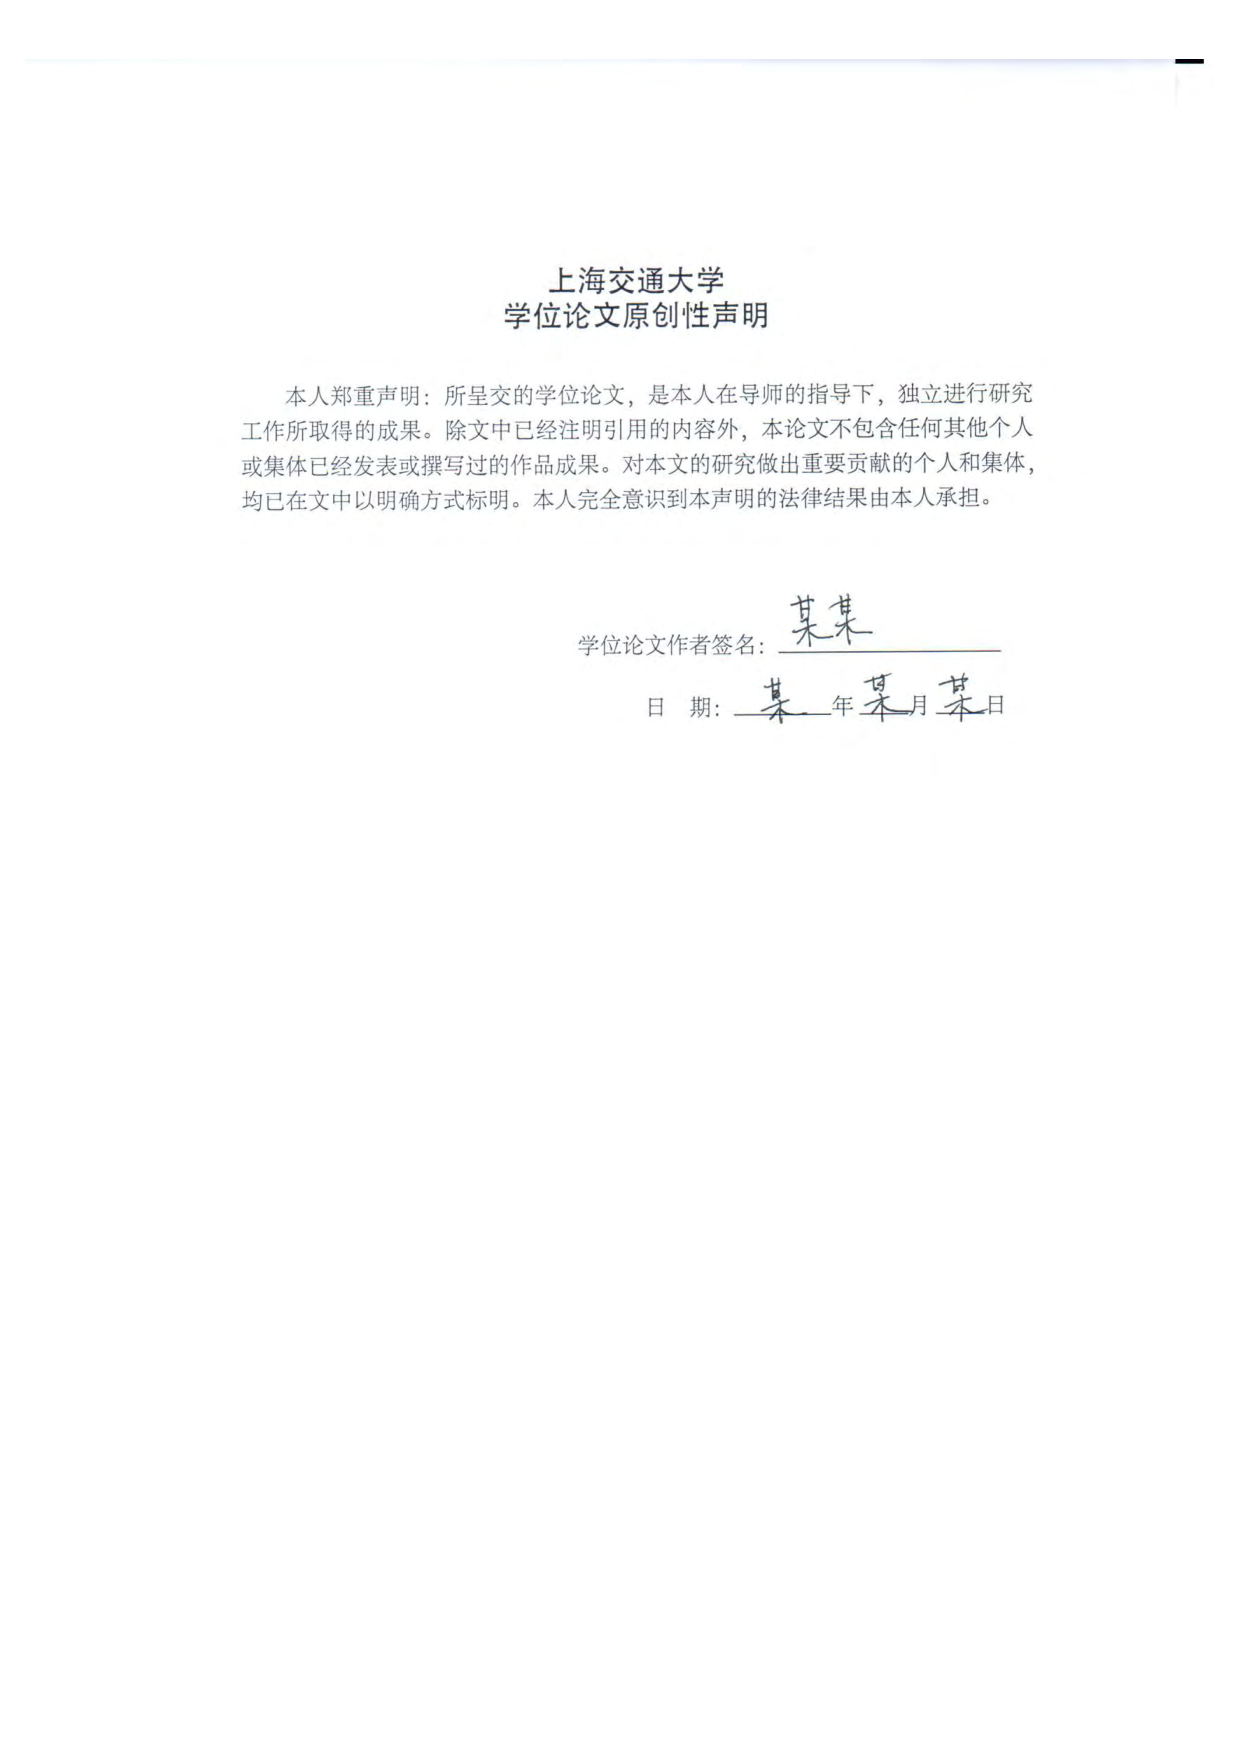
\includepdf{pdf/original.pdf}
	\cleardoublepage
	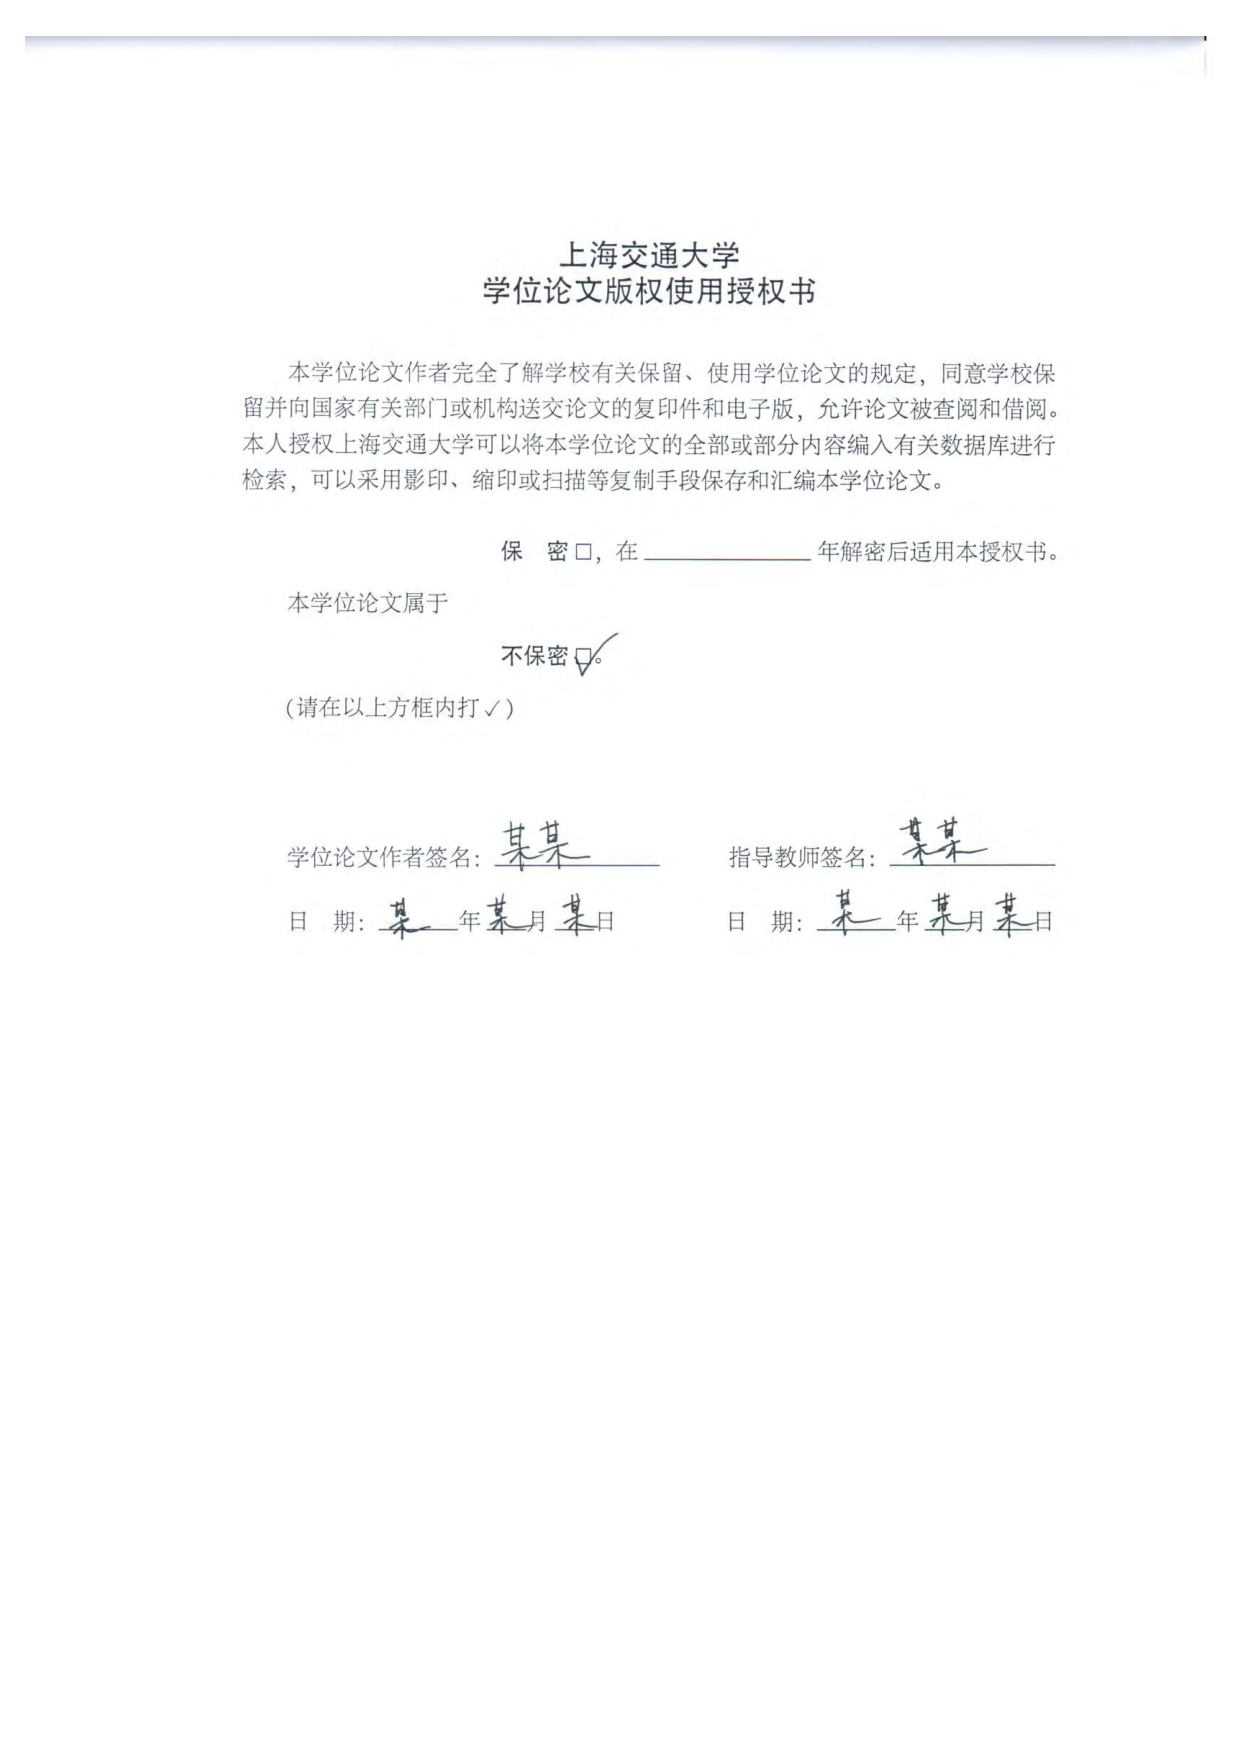
\includepdf{pdf/authorization.pdf}
	\cleardoublepage
\else
	\makeDeclareOriginal
	\makeDeclareAuthorization
\fi
\makeatother

\frontmatter 	% 使用罗马数字对前言编号

%% 摘要
\pagestyle{main}

%# -*- coding:utf-8 -*-
%!TEX root = ../thesis.tex
%%==================================================
%% abstract.tex for SJTU Master Thesis
%%==================================================

\begin{abstract}
\addcontentsline{toc}{chapter}{摘要}
无人水下机器人是人类探索海洋深处的一种有效工具,其在海洋中进行结构物或设施监测与作业的活动对水下机器人系统运行提出更加准确与稳定的要求。认识和操控水下机器人,尤其是欠驱动型水下机器人并不容易,无论是从本质上还是从便于实际操控上。水下机器人模型用来解释运动和施加在机器人上的力的关系,目前还没有一种通用的方法可以自动探索水下机器人本体模型的结构和参数。而由于机器人自身的驱动布置、形态重量和环境要素,水下机器人系统在水下环境中或者进行动态运动时呈现时变演化特点。并且,水下机器人所处的环境变化快、载体需可携带传感器设备、驱动器具有非线性以及一些意想不到的扰动与障碍都会使得控制系统运行变得不稳定。 因此, 探索性地研究水下机器人的模型与环境,并设计能够适应系统中的非线性、不确定性的鲁棒自适应方法就对水下机器人的理论和实践方面非常有必要。

本文围绕水下机器人模型的启发式搜索与非线性问题的鲁棒自适应控制进行展开,研究的重点放在具有复杂表达形式的水下机器人数学方程的结构与参数辨识以及考虑实践中的水下机器人的模型不确定性与驱动器非线性特点的水下机器人快速鲁棒自适应控制上。通过本文的研究,提出了一些有趣的水下机器人系统模型探索与系统控制方法,并进行大量的理论仿真对比与实验验证,为水下机器人的应用提供了理论与技术基础。本文的主要建模与控制贡献如下:

(1)针对水下机器人非线性系统的6自由度模型的结构与参数构成,提出了基于符号回归模型构建与探索方法。介绍了运动模型方程的基因树表达方法,并给出了符号回归中的模型表达树的演化过程。摒除了人类在研究模型的偏见与领域知识限制,揭示了蕴含在水下机器人运动数据集中的内在关系,让数据本身解释模型。从模型参数和结构两个角度,依赖获取的实验数据,建立精确的数学方程表达,发现新的模型结构,为认识与解决机器人的控制问题提供理论基础。

(2)考虑到水流环境的重要性,针对鱼雷型水下机器人不同的水流环境,基于鱼类侧线感知水流的机理,使用流体动
力学模拟载体受到的水流工况,选择使用线性判别分析的压缩感知处理方法进行数据降维、使用支持向量机分类方法训练并建立水流方向感知分类模型,并提出水流估计与惯导的融合框架,从功能角度验证了仿生侧线感应水流的能力,为水下机器人主动利用海洋环境提供理论基础。

(3)针对开发高精度模型的困难,并考虑到鲁棒控制目标应用中模型不确定项的影响,分别对两种不同的水下机器人(ROV、AUV)进行建模,其中ROV模型具有非初等几何表面形状复杂。使用计算流体软件分别计算流体动力学模型中的关键参数:附加质量项和阻尼矩阵项。针对具有理论公式描述的水下机器人系统,目标为自适应控制应用,使用泰勒展开方式对运动方程进行简化。给出了从外形和从数学两种不同的控制应用参考模型的确定方法。

(4)考虑到水下机器人系统特性:模型不确定性、非线性、各个自由度的耦合性、环境(盐度,机械冲击)中出现的干扰,给出了鲁棒自适应控制方法的基本控制架构以及稳定性判据。针对具有静不稳定特点的非线性6自由度水下机器人系统的俯仰控制问题,分别使用基于射影算子的模型参考自适应控制(MRAC)方法与 $L_1$ 自适应控制方法设计控制器。 通过控制实验对比,发现$L_1$ 自适应控制在响应速度和控制稳定效果上的优异性。


(5) 针对实际水下自治水下机器人平台控制中的时变模型参数以及驱动器的输入阈值、死区以及时变延迟的非线性特点进行理论分析,并基于模型参考自适应控制和$L_1$ 自适应控制进行设计可优化控制输出的抗饱和补偿器,将其用于水下机器人控制。实现了对静不稳定6自由度的自治水下机器人的俯仰、深度自由度的控制,验证了使用抗饱和补偿器优化鲁棒自适应控制方法的可行性。考虑多模式噪声与瞬态干扰、并与以往实验中使用的控制器进行对比,验证带有驱动补偿的$L_1$ 自适应控制方法的稳健而快速的控制性能。

本文主要展示了在水下机器人的建模与非线性自适应控制方面的理论研究,可以用于多种航行器系统模型的研究中,也可为人类在海洋活动中研究并应用水下运载器提供一种新的视角。

\keywords{\large 水下机器人 \quad 符号回归 \quad 系统辨识 \quad 模型探索 \quad 控制导向建模 \quad
$L_1$自适应控制 \quad MRAC \quad 抗饱和补偿器 }
\end{abstract}

\begin{englishabstract}
\addcontentsline{toc}{chapter}{Abstract}
Unmanned Underwater Vehicle(UUV) is an effective tool for the human to explore and exploit the deep ocean, which proposes more accurate and stable requirements for the development of the vehicle system when vehicles are utilized in many activities of the human being to discover ocean like inspecting underwater infrastructures or deploying submarine equipment. It is not easy to understand the underwater vehicle, especially the under-actuated underwater robots, in nature or manipulate it precisely in the exploration underwater. Models for the underwater vehicle are utilized to explain the relationship between movements and forces exerting on the robot. Yet currently there are no general methods can arrive a better model with structure and parameters for vehicle automatically in the discovery of model datasets. And considering the thruster configuration, the designed shape, and weight as well as the unknown underwater environments, the system described in mathematics or dynamic shows time-varying evolution in the model. Moreover, changes in the underwater environment, sensor instruments or actuators carried as well as some unexpected disturbances and obstacles in the operation will make the control system become unstable. Therefore, it is necessary to discover the modeling of a vehicle, perceive underwater surroundings, and develop a suitable controller that can adapt to nonlinearities, uncertainties in the vehicle system from the perspective of theoretical research and control applications.

In this thesis, the heuristic search of the underwater vehicle model and the robust adaptive control scheme of vehicle system with highly nonlinearities are carried out.  The research focuses on the model structure discovery and the parameters identification of the underwater vehicle, such as Remotely Operated Vehicle(ROV) and Autonomous Underwater Vehicle(AUV), as well as on developing excellent robust adaptive control approach where the uncertainties of the vehicle model and limitations of actuators are both taken into account. In this paper, some interesting approaches that can model the underwater vehicle via discovering datasets and controllers are proposed. Results from numerical simulations and experiments are both demonstrated and discussed, which proves to be an appropriate solution in theory and technique for further application in water. Contributions to the modeling and control of a vehicle in this thesis are listed as the following:


(1) Aiming at the difficulties of determining the structure and parameters of a nonlinear 6 Degree-Of-Freedom(DOF) underwater vehicle system, the symbolic regression used to investigate the modeling of the vehicle is put forward. Gene trees that can describe the movement mathematical equation are introduced. The evolution process of the model expressed in gene trees using symbolic regression method is also given out. Discarding the human bias in the study of the modeling for a vehicle and the limitations of knowledge in the field of expertise, the intrinsic relationship hidden in the measured datasets of a vehicle is revealed intelligently, which empowers the data the ability of self-discovery. Exact mathematical equation with new model structure is obtained using experimental data via investigating the structure and parameters of the model, which provides a new approach to re-understand the vehicle system and the basis for future controller design.

(2) Considering the effects of the water flow situation on an underwater vehicle, especially UUV, the motion of the vehicle in water is simulated using computed fluid dynamic(CFD) technique based on the mechanism of the fish lateral line that can perceive water flow. Linear discriminant analysis(LDA) method in the view of the concept of compressed sensing is employed to reduce the dimensionality of data. Support vector machine approach is utilized to train the water flow direction classifiers and the framework that fusing water flow forecasting and an inertial navigation system is proposed. In the thesis, the ability of vehicle identifying current like the fish lateral line is investigated in theory, which also provides a new point of view for an underwater vehicle to exploit ocean.

(3) Aiming at the difficulty of developing more accurate vehicle model and taking into account the effects of model uncertainties in robust adaptive control, the modeling for a vehicle like ROV, the shape of which is complex and composed of non-elementary geometry surfaces, and AUV in torpedo shape are investigated, respectively. Key terms like the added mass and damping matrix in the hydrodynamic model of underwater vehicle are both determined using CFD software. Oriented for the adaptive control, the nonlinear formula of the vehicle is simplified by using Taylor expansion method. The methods of determining the reference model for control from the outside shape and the theory mathematical expression are both put forward.

(4) Considering the characteristics of an underwater vehicle system, which mainly includes the uncertainties of the model, nonlinearities, the coupling relationship of each DOF and the interferences from the environment(salinity, mechanical shock), the basic diagram of the robust adaptive control scheme as well as the stability criterion are introduced. Aiming at the pitch channel control of a 6 DOF underwater vehicle system with static instability in water, the projection based model reference adaptive control(MRAC), as well as $L_1$ adaptive control scheme, are both used to deal with this problem. Performance results of control are demonstrated and it is found that the $L_1$ adaptive control surpass MRAC whether in the response speed or in the adaptability of control approach to stabilize the vehicle system.

(5) With the purpose of coping with the time-varying model parameters of AUV as well as the nonlinearities of actuators like input saturations, dead-zone, and time-varying delay, the anti-windup compensator is extended into the structure of MRAC and $L_1$ adaptive control to optimize the controller outputs. The attitude and position control of a 6 DOF underwater vehicle in the pitch channel and the depth mode are studied and simulated, which proves the effectiveness of the proposed control scheme. The robust and adaptive performances of $L_1$ adaptive control with anti-windup compensator are demonstrated and compared with the MRAC controller utilized in the experiments, where measurements noise, unexpected disturbance and limitations of actuators are considered.

The study on modeling and nonlinear adaptive control of an underwater vehicle are presented in this work. The methods proposed can be used in the research of various systems, and can provide a new perspective for the human being to investigate an underwater vehicle in theory and apply vehicle in the future exploration.



\englishkeywords{\large Underwater vehicle \quad Symbolic regression \quad System identification \quad Model discovery \quad Control oriented modeling \quad $L_1$ adaptive control \quad MRAC \quad Anti-windup compensator}
\end{englishabstract}



%% 目录、插图目录、表格目录
\tableofcontents
\listoffigures
\addcontentsline{toc}{chapter}{\listfigurename} %将插图目录加入全文目录
\listoftables
\addcontentsline{toc}{chapter}{\listtablename}  %将表格目录加入全文目录
% \listofalgorithms
% \addcontentsline{toc}{chapter}{代码索引}  %将表格目录加入全文目录

%%# -*- coding:utf-8 -*-
%!TEX root = ../thesis.tex
\chapter{主要符号对照表}
\label{chap:symb}

\begin{longtable}{rl}
$\epsilon$     & 介电常数 \\
 $\mu$ 		& 磁导率 \\
 $\epsilon$     & 介电常数 \\
 $\mu$ 		& 磁导率 \\
 $\epsilon$     & 介电常数 \\
 $\mu$ 		& 磁导率 \\
 $\epsilon$ 	& 介电常数 \\
 $\mu$ 		& 磁导率 \\
 $\epsilon$     & 介电常数 \\
 $\mu$ 		& 磁导率 \\
 $\epsilon$     & 介电常数 \\
 $\mu$ 		& 磁导率 \\
 $\epsilon$     & 介电常数 \\
 $\mu$ 		& 磁导率 \\
 $\epsilon$ 	& 介电常数 \\
 $\mu$ 		& 磁导率 \\
 $\epsilon$     & 介电常数 \\
 $\mu$ 		& 磁导率 \\
 $\epsilon$     & 介电常数 \\
 $\mu$ 		& 磁导率 \\
 $\epsilon$     & 介电常数 \\
 $\mu$ 		& 磁导率 \\
 $\epsilon$ 	& 介电常数 \\
 $\mu$ 		& 磁导率 \\
 $\epsilon$     & 介电常数 \\
 $\mu$ 		& 磁导率 \\
 $\epsilon$     & 介电常数 \\
 $\mu$ 		& 磁导率 \\
 $\epsilon$     & 介电常数 \\
 $\mu$ 		& 磁导率 \\
 $\epsilon$ 	& 介电常数 \\
 $\mu$ 		& 磁导率 \\
 $\epsilon$     & 介电常数 \\
 $\mu$ 		& 磁导率 \\
 $\epsilon$     & 介电常数 \\
 $\mu$ 		& 磁导率 \\
 $\epsilon$     & 介电常数 \\
 $\mu$ 		& 磁导率 \\
 $\epsilon$ 	& 介电常数 \\
 $\mu$ 		& 磁导率 \\
 $\epsilon$     & 介电常数 \\
 $\mu$ 		& 磁导率 \\
 $\epsilon$     & 介电常数 \\
 $\mu$ 		& 磁导率 \\
 $\epsilon$     & 介电常数 \\
 $\mu$ 		& 磁导率 \\
 $\epsilon$ 	& 介电常数 \\
 $\mu$ 		& 磁导率 \\
 $\epsilon$     & 介电常数 \\
 $\mu$ 		& 磁导率 \\
 $\epsilon$     & 介电常数 \\
 $\mu$ 		& 磁导率 \\
 $\epsilon$     & 介电常数 \\
 $\mu$ 		& 磁导率 \\
\end{longtable}
 % 主要符号、缩略词对照表

\mainmatter	% 使用阿拉伯数字对正文编号


%% 正文内容
\pagestyle{main}

%% 测试参考文献
% %# -*- coding:utf-8 -*-
%!TEX root = ../thesis.tex

参考文献测试区。
\cite{fossen1994guidance,fossen2011handbook,fossen1991nonlinear,clement2016modeling,haugen2012modeling,prestero2001verification,evans2004dynamics,Wu2012Hydrodynamic,dobrokhodov2008flight,lavretsky2013robust,dobrokhodov2008flight,wang2015numerical,gibson2015comparison,hovakimyan2010L1,Wu2012Hydrodynamic,jones2002calculation,Tang2009Estimation,perrault2003sensitivity,eng2014added,gibson2015comparison,garus2014thrust,muhammad2015flow,bouffanais2010hydrodynamic,tagliaferri2015wind,wunl2011immune,franosch2010biomimetic,abdulsadda2012artificial,yang2010artificial,jung2013flow,Wu2016lateralline,yang2014modeling,yang2015modeling,yang2015robust,huang2015trends,deng2009system,kim2012estimating,baruch2009levenberg,feng2006identification,luque2011auv}
\cite{hegrenaes2007comparison,hong2013online,sabet2014extended,wang2014sensitivity,xu2013identification,zhou2013genetic,chang2007nonlinear,dos2014genetic,dos2009nonlinear,Gandomi2012A1,Gandomi2012A2,menezes2014symbolic,schmidt2009distilling,schwab2012learn,stoutemyer2013can,wu2016parametric,Moreno2015Symbolic,Mcconaghy2008Genetic,wu2016parametric,shishengda1995submarine,yuanchuan2001submarine,lavretsky2013robust,lavretsky2010predictor,gregory2010flight,hyde2011flight,Dydek2015Adaptive,gibson2012improved,gadient2012very}
\cite{gibson2012adaptive,kharisov2010comparison,cao2010design,cao2008adaptive,Cao2006Design,Hovakimyan2008adaptive,cao2010stability,hovakimyan2010L1,Cao2006Design1,Luo2010L1,Cao2006Design2}
\cite{Cheng2008L1,Cao2008L1,Kaminer2010Path,holhjem2012l1,leman2010l1,dobrokhodov2008flight,wang2009l1,gregory2009l1,Zhiyuan2009Integrated,Lei2007Design,Guerreiro2009L}
\cite{Wise2008Verifiable,wang2008l1,aguiar2008time,kharisov2008l1,santhakumar2014robust,valladarez2015robust,valladarez2015adaptive,maalouf2015l1,sarhadi2014l1}
\cite{maalouf2012l1,maalouf2013new,maalouf2013stability,galeani2009tutorial,sofrony2010anti,folcher2004lmi,karason1993adaptive,kim2013variable,sarhadi2016adaptive1,sarhadi2016adaptive2,sarhadi2016model1,sarhadi2015state,sarhadi2017model2,enayati2016monte,dhurandher2008uwsim,rohmer2013vrep}

\cite{verschure2003environmentally,abdulsadda2013underwater,ren2012model,fan2002design,li2005design,jun2009development,wunl2011immune,yuan2010genetic,liu2012support,chen2000new,martis2013ecg}

\cite{menezes2014symbolic,garg2014mathematical,stoutemyer2013can,schmidt2010symbolic}

\cite{cui2016adaptive,hassanein2016model,wang2011l1,kharisov2014comparison,maalouf2012novel,oliveira2013design,sofrony2007anti,prestero2001development,yang2012observer}

\cite{alur1995algorithmic,park1999study,hsu2000dynamic,smallwood2004model,Sch2007an,aguiar2007dynamic,Souza2007Intelligent,madady2008pid,xu2008optimal,dukan2011dynamic,mellinger2011minimum,mellinger2012trajectory,dukan2013integration,li2015alignment,yoo2016path,allotta2016unscented,dos2016bank,dos2016bank,li2016precise,richter2016polynomial,hussain2017robustness,wang2016fast}

\cite{maalouf2013contribution}

\cite{wangbiao2016,wan2017CFD,wang2001rovcfd,feng2005intros,feng2010H_infty,xu2005simulation,xu2005deeprov,yangrui2015,yangke2014}

\cite{drake2016,russdrakebook,fantoni2002non,sutton1998reinforcement,tedrake2010lqr,tedrake2009lqr}

\cite{ardupilot,ardusub}


there are another references. \cite{aakre2016development,oien2016dynamic,knausgaard2013development,follestad2017autonomous,beinset2007controller,berg2012development,drozdik2015dynamic,lauritzsen2014hardware,eriksen2015horizontal,eidsvik2015identification,elgenes2017underwater,mu2017adaptive,arnesen20173d,lekkas2016online,fossen2015line,wiig2016integral,lekkas2013line,lekkas2014guidance,elmokadem2017terminal,candeloro2012observers,bertram2012practical}


%# -*- coding:utf-8 -*-
%!TEX root = ../thesis.tex
%%==================================================
%% chapter01.tex for SJTU Master Thesis
%%==================================================




\chapter{绪论}
\label{chap:Introduction}
% 1.1 研究背景及意义
% 1.2 水下机器人系统描述
% 1.3 水下机器人的控制特性以及研究进展
% 1.4 本文主要研究内容
% 1.4 本文的主要创新点
\section{研究背景及意义 }

地球表面积三分之二以上都是海洋,近三分之一以上的人类生活在近海和近河流湖泊地带。随着陆地水资源的不断消耗,对蕴含丰富生物资源与矿产资源的海洋的开发成为了人类生存与发展所关注的一个新的重要领域\cite{fossen1994guidance,Fossen2002Marine}。目前,世界各国愈发关注海洋探索,而作为其中探索率较低的水下世界,近年来越来越受到国家、企业等各种力量的关注,探索并开拓水下世界成为了国家、企业投资发展的一个重要战略组成\cite{bottaccini1954stablity,John1978Methods}。

\begin{figure}
\centering
\includegraphics[width=9cm]{figure/chap1/seadragon.jpg}
%\captionsetup{justification=centering}
\label{fig:chap1:F1}
\bicaption[fig:chap1:F1]{深海作业ROV-海龙 III}{深海作业ROV-海龙 III}{Fig.}{SeaDragon III ROV for observation}
\end{figure}

\begin{figure}
\centering
\subfigure[水下滑翔机]{
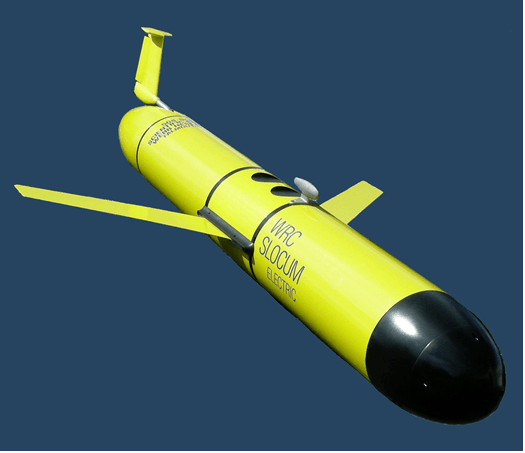
\includegraphics[width=6cm, height = 6cm]{figure/chap1/glider.png}}
\subfigure[REMUS 600型AUV]{
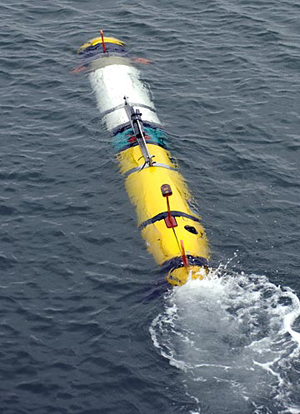
\includegraphics[width=6cm, height = 6cm]{figure/chap1/remus600.jpg}}
%\captionsetup{justification=centering}
\label{fig:chap1:F2}
\bicaption[fig:chap1:F2]{非缆控型水下航行器}{非缆控型水下航行器}{Fig.}{Underwater vehicle without cable}
\end{figure}

由于海洋环境与人类生存的陆地环境存在较大的差异,人类的科研与生产活动不能直接在水下实现。因此人类在探索、认识水下环境以及利用海洋中的资源主要借助于多种不同类型的水面、水下探测与作业设备来实现目标(如图\ref{fig:chap1:F1},图\ref{fig:chap1:F2}和图\ref{fig:chap1:F3}),其中图\ref{fig:chap1:F3}给出水下机器人贴近侧壁进行航行观测)\cite{oien2016dynamic,knausgaard2013development,drozdik2015dynamic}。水下机器人是一种目前世界上通用的一种较为先进的水下航行系统,其主要用于帮助人类对水下环境、结构物、海底管道以及其他水下设备进行观测和辅助作业\cite{fossen1994guidance,Fossen2002Marine,berg2012development,drozdik2015dynamic,feng2005intros}。水下机器人,又称水下航行器,主要由推进动力系统、能源管理系统、控制与通信系统和机械本体组成,其动力和控制可以由水面站进行供给和设置,也可由水下机器人本体压力舱内的便携电源管理系统和自动导航仪进行供电和运动导航\cite{fossen1994guidance}。

\begin{figure}
\centering
\subfigure[BLUEROV模型]{
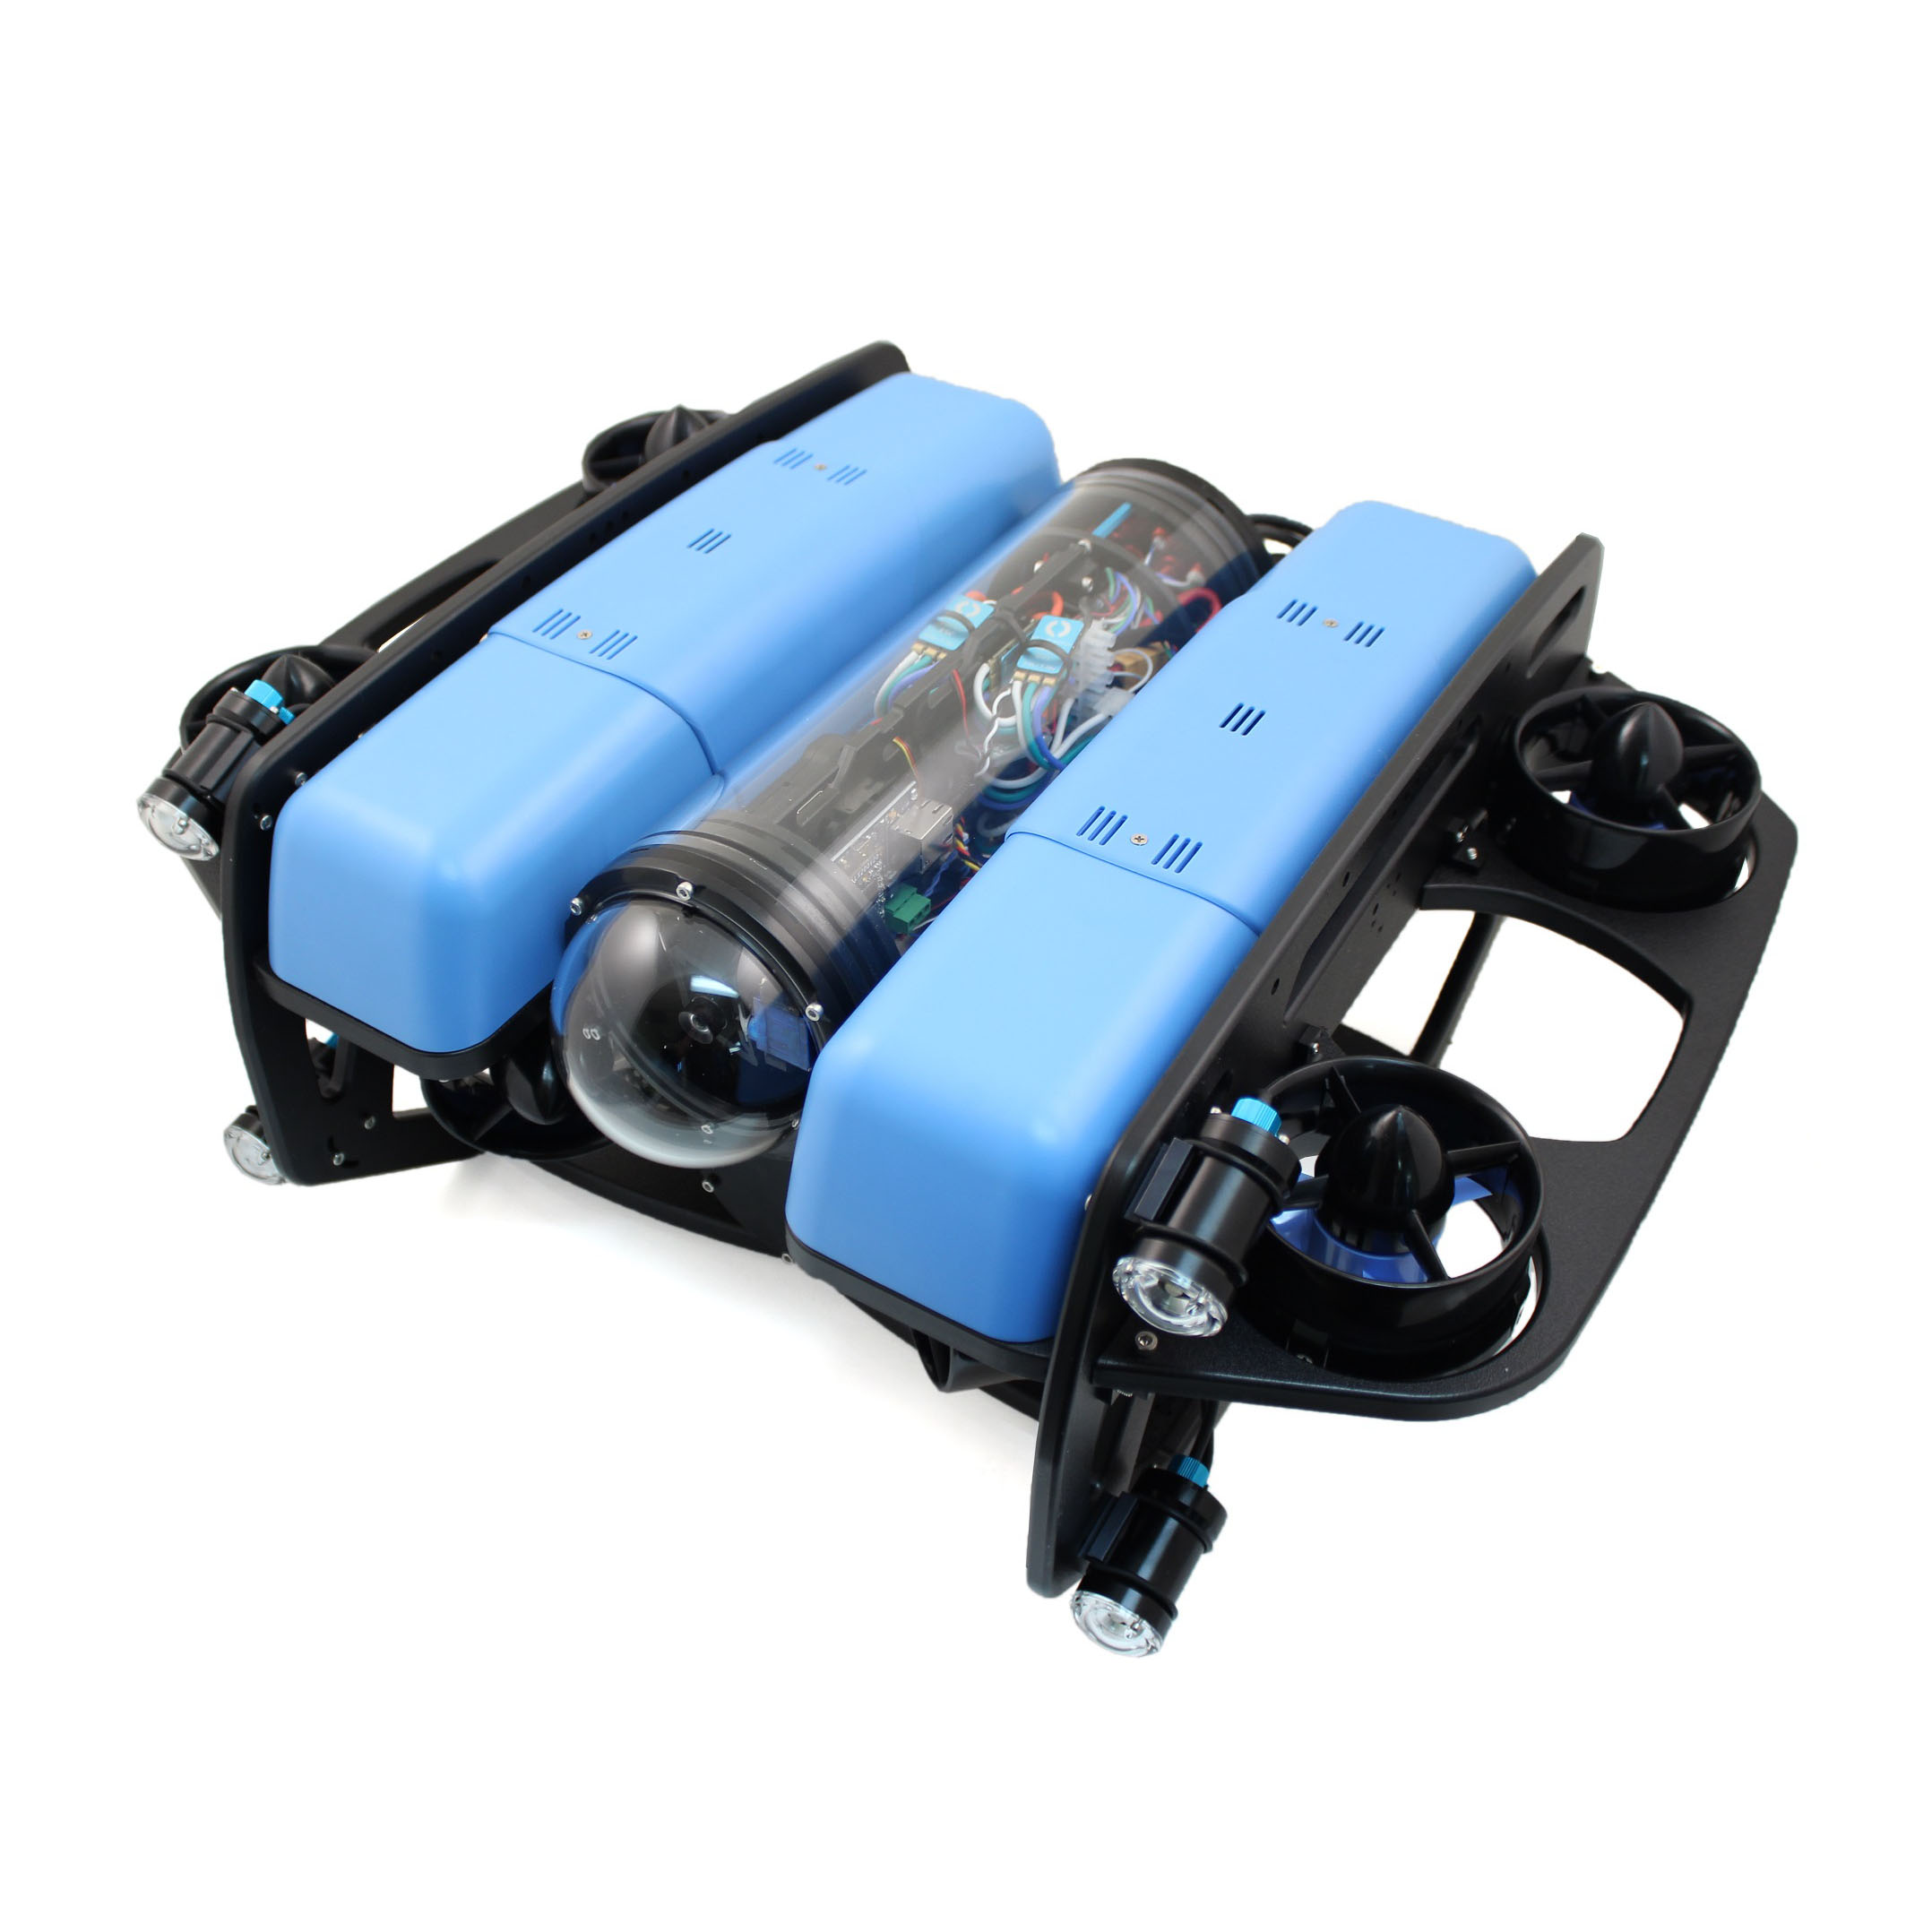
\includegraphics[width=6cm, height = 6cm]{figure/chap1/heavybluerov.jpg}
}
\subfigure[贴近侧壁观测]{
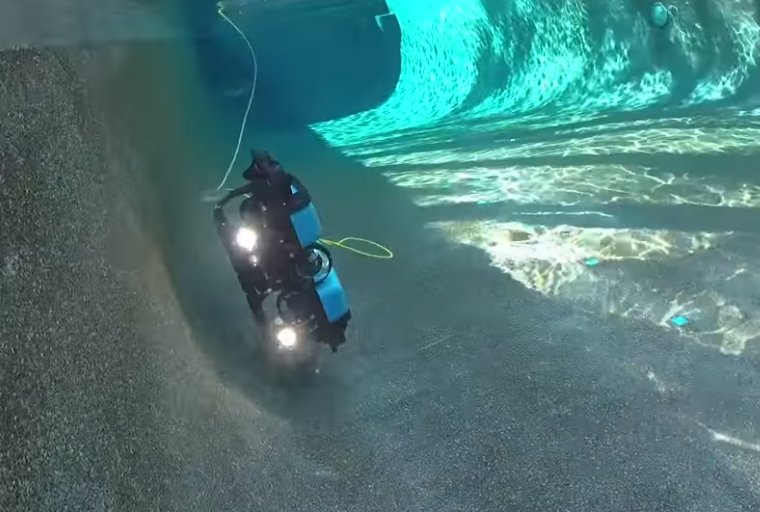
\includegraphics[width=8cm, height = 6cm]{figure/chap1/heavyblue.png}
}
%\captionsetup{justification=centering}
\label{fig:chap1:F3}
\bicaption[fig:chap1:F3]{小型缆控水下机器人BLUEROV}{小型缆控水下机器人BLUEROV}{Fig.}{Small ROV named BLUEROV}
\end{figure}


水下机器人根据控制方式不同,可以分为自治水下机器人(AUV)和有缆遥控水下机器人(ROV)。其中,由于带缆遥控潜水器(ROV)有着能在未知甚至危险的水下环境中完成长时间且相对可控的高强度、多形式的作业与观察的优异性能,因此ROV被广泛地应用在海洋水下环境的探索与开发活动中。ROV的应用主要集中在如下几个方面:海洋资源调查、海底海床绘制、海洋管道检测、水下矿物质或生物样本采样、以及未知水下领域的目标观测等\cite{follestad2017autonomous,aguiar2007dynamic}。AUV型水下航行器有着很强的自主性,能够到达的水下区域更加广阔,其主要用于海洋水质监测、水下资源探索、水生物观测、军事、水下传感器网络数据收发等\cite{maalouf2013contribution}。目前,水下机器人的探索开发应用有不断走向深海和远海的自主化趋势,为水下机器人的相关建模与控制技术带来了挑战\cite{wangbiao2016,yangke2014,yangrui2015,aakre2016development}。并且,由于水下机器人工作的水下环境具有高度复杂和强时变性,再加之水下机器人系统本身可能会因环境变化而产生不确定性,这些都会对水下机器人系统的运动稳定性与可靠性带来影响。因此,搜索并建立精准的水下机器人模型以及设计出考虑水下机器人非线性的鲁棒自适应控制的研究越来越受到国内外的学者关注\cite{yang2014modeling,haugen2012modeling,knausgaard2013development,eidsvik2015identification,eng2014added}。此外,水下机器人也可以基于动力学系统的控制输入个数与系统自由度的关系,研究不同动力布置的水下机器人的控制与动态系统的瞬态优化\cite{fantoni2002non,russdrakebook}。自然界中很多动态系统存在一些自由度没有控制输入,机器鱼、机器鸟虽然被设计开发出来,但是表现出来的性能与自然界所参考的生物本身相比,运动总是那么的不自然\cite{russdrakebook}。水下机器人的运动是通过设计状态反馈控制器来实现的,虽然可以达到控制目标,但是设计的运动大多忽略了系统本身的动态,例如系统中的非线性\cite{russdrakebook,galeani2009tutorial}。

水下机器人相关技术的研究如何,关系到水下机器人是否能够成功被应用于水下勘测、水下辅助作业、任务规划\cite{Souza2007Intelligent}。如何提高水下机器人的水下运动与导航性能的问题本身涉及的因素很多,其中对提高水下机器人系统整体性能起着关键作用的问题主要有水下机器人与环境模型的建立与识别、提高控制器对于模型非线性特性的自适应性与鲁棒性、考虑水下机器人设备所具有的驱动器非线性\cite{yang2012observer,sarhadi2016adaptive2}。水下机器人的模型用来解释本体运动与施加在本体上的力、力矩之间的关系,该模型对于控制和导航都具有重要作用\cite{wu2016parametric}。模型经常被用来观察水下机器人系统的状态,而因此水下机器人模型的准确性就很重要。水下机器人模型建立不仅仅是为了分析,也要更方便研究者和系统设计者的控制器设计工作。基于运动学和动力学的有关知识建立的水下机器人动力学模型是基于以往历史的理论认识,这种认识具有一定的指导性,但也具有一定的偏见性\cite{menezes2014symbolic}。水下机器人的模型包括数学模型的公式形式与具体模型参数\cite{schmidt2009distilling}。以往的系统辨识方法是基于确定的模型结构采用最小二乘法、遗传算法等优化搜索方法来辨识具体的模型参数,这种方法在模型结构确定的情况下具有较好的适用性与可靠性,但是机器人的动态系统从时间过程演化的角度来看,水下机器人的模型是否结构一直保持不变\cite{John1978Methods}?水下机器人进行系统参数辨识时,辨识的目标函数也是基于某种特定条件下的理论而得到的,随着水下机器人的运动不断进入到未知的区域,系统辨识的模型就可能会失去价值。系统辨识的前提一般是模型结构一定,然而没有一种方法能够自动地获取水下机器人模型的数学结构与参数\cite{wu2016parametric}。

对于被完全理解的系统所建立的模型可以很好的描述系统状态,然而水下机器人系统的非线性以及环境的未知性会对系统的搜索与确定带来困难。为了解决这一问题,启发式建模方法例如符号回归方法被用来搜索并确定水下机器人模型的映射关系与模型参数。由于用于进行模型参数学习和搜索的经验数据是在一定的实验条件下获取的,该数据获取方法的人力代价和实验成本都很高昂,且从成本上更加不适用于复杂形状的大型水下机器人(如图\ref{fig:chap1:F1})\cite{yang2014modeling}。为了快速而准确地获取水下机器人用于控制的模型,参数辨识、模型简化以及数值建模技术被用于本文的研究。由于水下机器人的运动具有高度非线性并且受到不确定性的扰动影响,在设计水下机器人的控制器时,需要给线性动态系统中添加不确定性和未建模动态\cite{valladarez2015adaptive}。水下机器人的控制器设计时要保证两个原则:鲁棒性和自适应。鲁棒性可以保证水下机器人系统在意外最坏情况出现时而不失效,自适应性可以保证水下机器人系统可以更好地适应环境中的不确定性与干扰。水下机器人动态系统的非线性包括一般非线性(模型参数时变、模型结构变化)和特殊非线性(驱动器阈值、死区特性)\cite{Wu2018Pitch}。鲁棒自适应控制虽然是为了解决模型的不确定性而设计,但是它不是所有问题的万能解决方案\cite{lavretsky2013robust}。因此,为了确保水下机器人的工作性能,在设计水下机器人的控制器是需要考虑水下机器人的驱动器的非线性特点,使用现代补偿器控制策略来对自适应控器进行优化,以保证水下机器人的控制性能。

综上所述,本文研究搜索水下机器人的数学结构与模型参数、建立用于控制机制的水下机器人模型并设计带有输入饱和补偿特性的鲁棒自适应控制器,可为水下机器人系统的智能应用提供参考。

% \section{水下机器人系统研究现状  }

\section{水下机器人系统建模研究现状 }

本研究分别从运动动力学理论建模和数据驱动的建模两个角度展开,主要包括水下机器人的运动动力学建模与关键项计算、基于实验数据的数学模型的结构表达搜索与参数辨识以及水下机器人对于环境水流的感知。水下机器人的空间运动建模主要有两种方法:一是根据推进器推力布置,基于牛顿运动定律进行的建模,其中有阻尼、附加质量等;第二种方法是采用系统辨识方法对获得的实验数据进行参数辨识,根据选择的模型结构与公式,确定相关水动力参数;第三则是水下机器人的建模是有其应用目标的,基于控制应用的导向,采用数值计算方法与模型简化获得用于非线性自适应控制的方程。

\subsection{水下机器人的动力学运动学建模  }

通过对水下机器人进行运动与动力学分析,国外学者Fossen 系统地给出了AUV和ROV类型的水下航行器的流体动力学模型\cite{fossen1994guidance}。我国学者施生达、元泉等也基于潜艇理论可以将水下机器人的模型进一步划分为水平面模型和垂直面模型\cite{yuanchuan2001submarine,shishengda1995submarine}。

水下机器人形状和类型各异,这使得水下航行器的流体动力学模型中的各项所起的作用也会有所不同,在使用时应对水下机器人的模型进行一定的处理。根据水下航行器的类型与运行特点可提出一些假设,用于简化水下机器人的动力学模型\cite{Fossen2002Marine,fossen1994guidance,fossen2011handbook,yangke2014}。水下机器人模型虽然在使用的时候都会被简化处理,不过简化后的模型结构以及简化后用于求解模型参数的方法好坏仍然不同。AUV和ROV的简化模型现已经被广泛用于AUV、ROV的运动控制与导航规划中\cite{clement2016modeling,haugen2012modeling,prestero2001verification}。具体而言,在使用Fossen建立的运动动力学模型时,如何针对不同类型形状和应用目标的水下机器人进行流体动力学计算以确定模型中的参数成为一个富有意义却又实际的问题。为了整体地评估所设计的水下机器人的流体动力学性能,Evans在文中描述了自主水下航行器的动力学模型并使用流体力学计算方法评估了本体所受到的力以评估所设计的航行器的性能\cite{evans2004dynamics}。
水下机器人的外形不同,一般可以划分为流线型和复杂形状,因此不同航行器流体动力学性能计算的困难和速度也不同。而根据流体对本体作用的机理不同,研究者也分别从非初等几何复杂形状、附加质量、阻尼、流线型设计与性能角度展开了流体计算研究\cite{Wu2012Hydrodynamic,jones2002calculation,Tang2009Estimation,wan2017CFD,wang2001rovcfd}。Tang\cite{Tang2009Estimation}使用计算流体动力学用来估计具有复杂形状的水下机器人的流体动力学系数,并通过与实验结果对比验证计算所得的参数值。Wang\cite{wang2015numerical},Perrault\cite{perrault2003sensitivity}和Eng\cite{eng2014added}使用流体动力学软件(WAMIT)计算框架式ROV、 AUV的附加质量参数并通过实验验证计算的参数值的准确性。 Gibson\cite{gibson2015comparison}提供八个不同的流线型AUV模型,并使用最小二乘法和自适应辨识方法来近似估计阻尼模型的系数,通过对比,确定出哪个模型的线性阻尼性能更加优秀。

在运动动力学模型中,Garus\cite{garus2014thrust}介绍水下机器人的推进系统的推力分布方法,并根据运动要求和系统无故障的设定进行推力分布的优化,这对于理解设计水下机器人系统也很有益。本文中尝试建立了一种推力控制矢量用来表达每个推进器对整体控制的影响,以便于控制器的整体设计。此外,如何感知海洋运载器的环境要素在近年也受到研究者的关注\cite{muhammad2015flow,bouffanais2010hydrodynamic,tagliaferri2015wind}。设计小型水流侧线系统,并将系统装到水下机器人原型中,实验验证系统的可行性\cite{franosch2010biomimetic,abdulsadda2012artificial,yang2010artificial}。Jung\cite{jung2013flow}基于水下鱼类的侧线器官的水下环境感知机理,提出使用压力传感器网络来辅助控制,并使用二维平面运动分析流体动力学。本课题研究者针对鱼雷型UUV的不同的水流环境,基于鱼类侧线感知水流的机理,使用流体动力学模拟载体受到的水下情况,选择使用线性判别分析和支持向量机技术进行数据降维、训练以建立水流方向感知分类模型,从功能角度验证了仿生侧线感应水流的能力\cite{Wu2016lateralline,friedman2001elements}。
为了将水下机器人模型的建模工作与控制实践联系起来,Yang, Benoit和本课题作者对具有模型不确定性的水下机器人鲁棒控制的关键问题进行了研究\cite{yang2014modeling}。其中,在对具有复杂形状的AUV的模型建立进行研究时,开发准确的流体动力学模型受到高成本问题的制约,这为缩小模型的不确定性以提高控制的性能带来很大困难。该文作者使用流体计算软件对于低速AUV CISCREA进行面向控制的建模预测流体动力学关键参数:附加质量和阻尼矩阵\cite{yang2014modeling,yang2015modeling}。并且,在论文中研究者使用建立的模型进行$H_{\infty}$鲁棒控制方案设计,并用于偏航控制的实验验证\cite{yang2015modeling,yang2015robust,du2016robust}。


\subsection{数据驱动的系统建模 }

基于数据驱动的建模方法\cite{huang2015trends},目前主要是采用系统辨识,该方法需要确定所研究对象的数学表达结构,而近年来,研究者使用了多种方法进行非线性系统的辨识研究\cite{deng2009system}。Kim\cite{kim2012estimating}等人提出了一种无需模型的方法来估计自由飞行物体的动力学,使用非线性回归方法和局部投影回归方法,对乒乓球体运动进行实时跟踪估计,并使用EKF来增强估计模型的鲁棒性。Baruch\cite{baruch2009levenberg}提出一种新型的循环神经网络模型用于系统辨识, 并使用反向传播 和递归Levenberg-marquart算法用于估计自适应控制的状态。Feng\cite{feng2006identification}为解决岩石的应力非线性表达问题,提出一种改进的粒子群优化的遗传算法对岩石的材料模型结构和相关参数进行系统识别,该方法可以同时识别模型的结构和参数。在海洋运载器的研究上也有大量的研究者从事探索\cite{luque2011auv,hegrenaes2007comparison,hong2013online},其中Sabet\cite{sabet2014extended}提出了一种用于估计水下机器人的流体动力学系数的方法,分别使用了扩展卡尔曼滤波和无迹变换卡尔曼滤波方法来辨识具有强非线性的水下机器人的模型的参数,结果发现UKF要优于EKF。Wang\cite{wang2014sensitivity}与Xu\cite{xu2013identification}分别使用4自由度的船舶操纵数学模型和6自由度运动模型获得实验数据,通过分析数据,使用SVM回归方法确定模型中的流体力学系数,通过将预测结果与实际对比,以证明方法的有效性。
其中,来源生物进化的遗传算法也被用于研究非线性系统辨识问题,Zhou提出基于遗传算法的时域识别算法,通过将遗传算法(GA)应用于分阶系统的识别\cite{zhou2013genetic}。Chang提出一种应用于非线性系统的识别和控制的遗传算法,尝试使用实际编码来描述系统,假定结构的情况下,估计系统模型\cite{chang2007nonlinear}。为了更好的将系统辨识的目标方程在生物进化中更好地表达,Santos采用基因编程(GP)方法的树状结构被用来描述识别问题,并使用该方法辨识提升阀的进气口与排气口的数学关系,将GP方法用于系统识别的结构选择问题,通过自动修改基因表达树的结构和组成,以此来辨识非线性的球管系统\cite{dos2014genetic,dos2009nonlinear,Mcconaghy2008Genetic}。Gandomi提出一种新的方法,使用多基因遗传规划方法来研究经典回归辨识中的非线性模型的互相作用问题,并在复杂的结构工程问题中进行实例验证说明\cite{Gandomi2012A1,Gandomi2012A2}。
虽然系统辨识可以用来确定非线性模型的系数,但是它的研究会基于一个前提,即已知的数据表达的假设,所限制,这对于人类进行快速有效的自动建模是一种阻碍\cite{menezes2014symbolic}。符号回归是一种回归分析,它从精确度和结构演化两个方面搜索数学表达式的空间,以找到最适合给定数据集的模型,该方法并没有提供特定的模型作为算法的起点。相反,通过随机组合数学建模功能块(例如数学运算符,分析函数,常数和状态变量)来形成初始表达式,然后通过使用遗传编程重组前述方程形成新方程\cite{schmidt2009distilling,wu2016parametric}。
受自然启发的机器学习技术如符号回归方法、稀疏回归等启发式搜索方法被用来从经验数据中自动学习模型用于研究复杂的网络现象\cite{menezes2014symbolic,brunton2016discovering}。为解决寻找自然规律和数学方程的过程不能自动化的问题,Schmidt提出一个确定非重要性原则,并通过从数据集中自动搜索运动方程以验证所提出算法的有效性\cite{schmidt2009distilling,schmidt2010symbolic}。Schwab提出一个灵活的知识表示框架,它利用符号回归学习和数学表达式来从数据中获取规律,该算法可以通过挖掘数据以产生新的规律描述,并添加到知识库中用来提高整体的学习性能\cite{schwab2012learn}。
由于不要求指定特定模型,符号回归不受人类偏见或领域知识中的未知空白的影响。它试图揭示数据集的内在关系,通过让数据中的模式本身揭示适当的模型,而不是强加从人类视角在数学上易于处理的模型结构。这有助于推理,并有利于获得有关数据,以生成对系统的洞察。Eureqa软件从数据中生成清晰的数学表达式,并根据表达式结构是否已知,可以分别搜索模型的数学结构和精确地拟合出模型,进而可以计算模型的参数\cite{stoutemyer2013can}。在对水下机器人的建模中为了更好了解实际运动中的各个变量的数据集的映射关系,本课题的研究者使用实验数据,选择使用基于自然选择的符号回归方法,自动地检测水下机器人本体的数学结构,并且所提出的方法也可以用来辨识模型参数,且性能经过与Levenberg-Marquardt算法和遗传算法对比,以验证提出的方法的有效性\cite{wu2016parametric,Moreno2015Symbolic}。


\section{非线性自适应控制现状 与水下机器人控制特性 }

自适应控制律和参数更新律往往是直接基于线性的无干扰、无噪声、无未建模动态的动态系统来设计的,这种控制方法容易开发,但是在实际应用中会与实际系统的模型不一致而给控制带来偏差。一个受控制系统如果因为系统是非线性的,它的参考模型是低维度的,且实际控制的系统是高维度的\cite{russdrakebook}。控制参考模型系统与实际系统之间的偏差会影响水下机器人系统的稳定性与运载器的轨迹追踪性能\cite{li2005design,jun2009development,garcia2014modelling,wang2016fast}。为了更好地设计出适用于实际系统的控制器,水下机器人的控制系统必须要靠非线性、未建模干扰、有界噪声等因素,并使用接近于现实的复杂非线性全自由度模型系统进行验证。

非线性自适应控制的具体设计主要是控制器的设计考虑了模型的多种不确定性以及有界的干扰。有些自适应控制器在存在小干扰的情况下会变得不稳定,出现参数漂移问题。这非常的糟糕,也曾在学术界引起的了讨论。许多人员从自适应控制器的设计的多种角度进行分析和研究,试图找到自适应控制器的不稳定的原因以及消除不稳定的方法。设计出稳定的自适应控制方法并可适用于实际系统的指令跟踪,即产生了鲁棒自适应控制的设计方法。鲁棒自适应控制的目的是为了解决动态系统中存在的模型不确定性和扰动,Lavretsky 和 Ioannou 试图从多个不同的角度来分析不稳定机制,并对存在的自适应控制方法进行修改,以期得到可以适用于广泛动态系统的自适应控制方法,并最终在实际系统中应用此方法,如飞机\cite{lavretsky2013robust,Ioannou2012}。

在水下机器人系统的控制设计中,首先是要获得准确的航行器系统描述。然而,实际的海洋机器人系统因为工作的水下环境的复杂多变而具有较大的不确定性。水下机器人的建模需提供准确的模型用于设计,这样的模型既要能够表征系统的主要运动特征又不能太过复杂,使得控制器的设计变得异常困难\cite{fossen1991nonlinear,beinset2007controller,eriksen2015horizontal}。过度简单的模型虽然容易控制但是寻求控制器最优解的过程会变得过于漫长,又或者设计的控制器的调参要耗费很大的精力\cite{sutton1998reinforcement,madady2008pid}。本文的研究尝试使用鲁棒自适应控制的基础方法来分析水下机器人的位姿控制问题,根据鲁棒控制器中具体模块部分的设计要求的不同,分别对参考模型的更新与动态更新,自适应律的计算稳定性与速度以及水下机器人的系统非线性特征进行研究。


\subsection{鲁棒自适应控制的研究进展  }


鲁棒控制可看作一种在线控制策略,它能对可能包含有界不确定性的系统进行调节校正,该方法往往利用反馈-前馈状态输出关系产生相应的控制输入,从而使设备输出沿预定的“轨迹”变化,自适应控制对过程不确定性进行在线估计,然后产生控制输入以预测、克服或者尽量减少相对于预期闭环设备行为的不利偏差,可以将自适应控制看作是线性反馈积分器的非线性拓展\cite{lavretsky2013robust}。大多数的实际系统中,纯粹的鲁棒控制或者是自适应控制都不能做到更好的效果,因为系统总会有不确定性和非线性情况,而将两者结合是一种有益的尝试,也得到了诸多研究者的关注。

基于传统的模型参考自适应框架,Lavretsky系统性地研究鲁棒自适应控制,其中状态反馈直接模型参考自适应控制和具有积分反馈的模型参考自适应控制方法在航行器上的应用具有实用意义,并且为了抑制有界扰动,可以使用射影理论对模型参考自适应控制(MRAC)进行设计\cite{lavretsky2013robust}。Lavretsky基于预测器进行模型参考自适应控制设计,并将其与传统的模型参考自适应控制进行对比,仿真验证所提出的控制器能改进瞬态特性\cite{lavretsky2010predictor}。 在航空航天应用中,鲁棒自适应控制也得到了实践验证\cite{gregory2010flight,hyde2011flight}。 在低成本的四旋翼飞行器上,模型参考自适应控制用于对线性控制器进行增广,并且使用Lyapunov稳定性理论证明控制器的稳定性,该方法可以应对推力损失带来的不确定性\cite{Dydek2015Adaptive}。 基于模型参考的自适应控制响应特性也得到关注,射影理论被用于改善自适应的瞬态性能\cite{gibson2012improved}。 Gibson对闭环系统的直接和间接模型参考自适应控制的鲁棒性、稳定性以及瞬态性能进行了分析\cite{gibson2012adaptive} 。此外,随着技术发展,柔性飞行器的控制问题也采用自适应方法用于解决本体的挠度问题\cite{gadient2012very}。这些研究表明了自适应控制对于解决科研中热点问题的潜力。

基于MRAC架构的鲁棒自适应控制被用于非线性系统的控制,并且与不同的控制架构的非线性自适应控制性能也进行了对比\cite{kharisov2010comparison,kharisov2014comparison}。相比于MRAC框架,$L_{1}$自适应控制(L1AC)作为一种新的控制理论在瞬态性能、自适应估计不确定性和干扰、稳定性都被进行了理论证明\cite{Cao2006Design,cao2008adaptive,cao2010stability,wang2011l1,Hovakimyan2008adaptive}。此外,Hovakimyan在著作中全面阐述了开发的L1AC的控制理论,该方法的关键特点就在于将适应性与鲁棒性解耦,以提高自适应控制器的瞬态性能和鲁棒性\cite{hovakimyan2010L1}。Cao提出一种新颖的自适应控制框架,该框架下确保了控制器的输入输出两个信号的同时有界瞬态性能,其中该控制依靠低通滤波器与小增益定理来证明控制架构的稳定性,并对自适应控制最重要的非线性和模型不确定性都进行解决\cite{cao2010design,Cao2006Design1,Cao2006Design2,Cheng2008L1,Cao2008L1}。而在实践中,Kaminer通过设计一种三维空间的路径跟踪算法并使用商用的飞控将L1AC控制从理论带入实践中,验证了L1AC框架的优越性\cite{Kaminer2010Path}。Holhjem,Leman分别研究了F16和X-48B飞机在存在明显耦合的动力学和控制的纵倾和控制面失效下的L1AC控制实践\cite{holhjem2012l1,leman2010l1}。Dobrokhodov实施$L_{1}$自适应控制器在飞控上的故障恢复\cite{dobrokhodov2008flight}。NASA AirSTAR\cite{gregory2009l1}、空中加油\cite{wang2009l1,Wise2008Verifiable}、超音速飞机\cite{Lei2007Design}、油井钻进系统\cite{Zhiyuan2009Integrated}以及多种航行控制器系统的设计与验证\cite{dobrokhodov2008flight,wang2008l1,aguiar2008time,kharisov2008l1}中均采用$L_{1}$自适应控制解决问题。这些都证明了L1AC控制框架的优越性。

而在海洋机器人上,自适应控制问题也受到了诸多研究者的关注\cite{wang2016fast,hassanein2016model}。Fossen对早期的水下机器人非线性控制问题进行研究,文中作者针对水下机器人的线性速度不能获得问题,设计了一种非线性观测器来对线性速度进行状态估计,并使用3自由度的AUV模型来展示设计的自适应控制律的收敛性和鲁棒性\cite{Fossen2002Marine,fossen1994guidance}。 Santhakumar使用模型参考自适应控制对水下载体操纵系统进行跟踪控制,提出的自适应控制方法在线估计了未知参数并补偿到系统中,如此机械手的工作对于水下机器人系统的影响通过自适应控制得以估计\cite{santhakumar2014robust}。Valladarez对水下机器人与潜水员合作所带来的联合动态操作问题进行了研究,水下机器人的精确控制需要准确的描述载体的模型,但是由于机器人载体配置或者受不确定因素的影响导致获得准确的模型比较困难,文中使用MRAC和L1AC控制对悬停的水下机器人系统进行升沉控制研究\cite{valladarez2015robust,valladarez2015adaptive}。近两年来,随着L1AC在航空飞行器行业的实践验证,L1AC也得到水下机器人的研究者的关注\cite{maalouf2012novel,sarhadi2014l1}。Maalouf首次在水下机器人领域引入L1AC架构,该控制方法对自适应控制的鲁棒性和自适应性进行解耦从而实现高适应增益,文中作者将非线性状态反馈控制器(ANSF)和$L_{1}$自适应控制进行比较研究,针对不同的情况进行AC-ROV试验研究,从而突出了使用L1AC方法的优越性\cite{maalouf2015l1,maalouf2012l1}。而后,Sarhadi对鱼雷型AUV的俯仰姿态进行了$L_{1}$控制器设计,在存有有界扰动和不确定性的条件下,使用仿真模拟验证了L1AC的控制性能\cite{maalouf2012l1}。 Maalouf对小型低配置航行器的控制问题进行了研究,对于存在的许多干扰和建模不确定性的俯仰角度控制,作者从理论的角度进行了$L_{1}$非线性自适应控制分析,Maalouf还对L1AC框架中具有时变参考轨迹的内部延时观测问题进行了论证研究,通过使用L1AC对原有的PID控制器进行增广控制以减少追踪延迟\cite{maalouf2013new}。 此外, Maalouf对L1AC用于小型水下机器人的稳定性进行了理论分析并试验验证方法的有效性\cite{maalouf2013stability,maalouf2015l1}。




\subsection{驱动器饱和补偿问题的研究进展  }

近年来,水下机器人系统应用越来越广泛,而实践上使用的驱动器的特点也为控制应用带来研究点。驱动器无论是舵片还是螺旋桨推进器都是具有界限的,这本质是一种饱和非线性。为此,抗饱和补偿器的研究也得到诸多关注\cite{galeani2009tutorial,Turner2017Positive,sofrony2010anti}。Galeani提出了线性和非线性的抗饱和补偿器,并分析了不同方法补偿的优缺点\cite{galeani2009tutorial}。针对带有限速执行器的系统开发了一种抗饱和控制方法,该方法使用Riccati方程进行设计全阶抗饱和补偿器且具有计算负担低适用性强的特点\cite{sofrony2010anti}。对于存在螺旋桨饱和情况下的水下机器人转向控制,Folcher使用LMI设计过程优化超过饱和阈值和没有超出饱和阈值的控制输出问题\cite{folcher2004lmi}。

在确定控制方案后,将抗饱和补偿与原来的控制架构进行融合的问题也得到了诸多研究者关注\cite{oliveira2013design,sofrony2007anti,Chen2009Neural}。Karason研究了控制应用中普遍存在的数控有界限问题,并通过分析提出了自适应控制中的确保不确定性和外部干扰带来的自适应控制有界的条件\cite{karason1993adaptive}。对具有驱动器饱和的PID控制性能进行研究,Kim提出一种抗饱和的双环路变结构PID控制器,并在水下航行器上进行应用分析\cite{kim2013variable}。尤其近一年来,水下航行器实际特点与模型参考自适应的结合研究也成为了研究的热点。Cui系统地给出了滑模控制用于解决具有驱动器非线性鱼雷型水下航行器的姿态控制问题,其中死区、阈值被进行了系统性的研究\cite{cui2016adaptive}。Sarhadi论述了存在驱动器饱和的非线性水下航行器的自适应控制问题,使用修正的MRAC控制器以保证驱动器在具有输入饱和时的合适的性能\cite{sarhadi2016adaptive1}。为解决水下机器人本体中存在的驱动器饱和问题,将Riccati抗饱和控制器融合到具有积分反馈的MRAC控制中,并使用提出的方法对REMUS的转向和俯仰进行姿态控制\cite{sarhadi2016adaptive2}。为了优化实际运行中水下机器人的控制行为,且对工业中普遍使用的PID控制应对饱和发生时性能降低的问题,通过将抗饱和补偿器与PID组合,用以改善控制器的输入输出,模拟验证了所提出方法的有效性\cite{sarhadi2016model1}。

水下机器人控制算法验证,需要更好地利用水下机器人的仿真和调试平台。为了验证设计的算法,Sarhadi为AUV提出了一种具有抗饱和补偿效应的新型模型参考自适应控制并根据所提出的控制器在AUV中使用硬件在环仿真验证所提出方案的有效性\cite{sarhadi2015state,sarhadi2017model2,hsu2000dynamic}。Lauritzsen 为深海ROV SF 30K 开发了用于测试水下机器人控制方法的硬件在环平台, 方便了动力定位的算法开发\cite{lauritzsen2014hardware,smallwood2004model}。{\O}ien基于Qt和MATLAB语言开发了自主无人船对的动力定位程序用于测试控制算法,为进行水下机器人测试提供了参考\cite{oien2016dynamic}。Tedrake 和 BlueRobotics公司分别开发了DRAKE机器人算法平台和基于Ardusub仿真算法可以用于水下机器人进行控制算法、路径规划、航点跟踪的系统仿真软件框架,便于水下机器人进行控制算法开发与测试,并可进行软件在环的仿真\cite{drake2016,ardusub,ardupilot,arnesen20173d,rohmer2013vrep,tedrake2009lqr,tedrake2010lqr}。 此外,为分析高度非线性和模型不确定项对水下航行器的行为影响,Enayati使用蒙塔卡洛方法建立水下机器人的6自由度模型,其中包括了流体动力学和附加质量项,控制仪器(传感器和驱动单元)、环境条件和初始条件\cite{enayati2016monte}。为了更好地进行控制器的实践工作,ROS机器人操作系统可以方便的将控制节点与电机数据发送节点、传感器节点相结合从整体实验和仿真上验证方法的有效性\cite{dhurandher2008uwsim,xu2005simulation}。


\section{本文主要研究内容 与拟解决的关键问题 }

\subsection{本文的主要研究内容 }

本文结合水下机器人在海洋中应用所需要解决的关键技术问题,开展水下机器人建模与控制器开发的调研工作;依据不同的水下机器人技术对航行器在水下运动、勘测与导航等问题的重要性,针对性地提出搜索水下机器人的模型并予以构建、提高水下机器人控制器对于多种不确定性的适应度、稳定地应对机器人系统运行中的意外情况以及考虑驱动器的非线性特性的控制补偿的相关研究工作;通过本文的工作,给出不同驱动类型的水下机器人的动力学建模与推力布置模型,为水下机器人的数学模型搜索与系统辨识、鲁棒自适应控制用的模型建立、控制器设计提供了理论基础,也为水下机器人的工程实践提供一定的参考。围绕水下机器人的建模、非线性自适应控制两大关键模块,主要从如下几个部分依次展开:

%%%%%%%%%%%%%%%%%%%%%%%%%%%%%%%%%%%%%%%%%%%%%%%%%%%%%%%%%%%%%%%%%%%%%
第一章论述课题的研究背景与意义、水下机器人的系统的研究现状,对于水下机器人的建模与控制相关的国内外研究现状进行分析与总结,重点拟出水下机器人的建模中的模型搜索、水下感知、控制用建模以及存在多种非线性和干扰时的水下机器人控制问题,并给出全文的研究路线。

%%%%%%%%%%%%%%%%%%%%%%%%%%%%%%%%%%%%%%%%%%%%%%%%%%%%%%%%%%%%%%%%%%%%%
第二章系统地引入一般形式的水下机器人的坐标系、运动学状态转换方程、流体动力学模型。提出将水下机器人分为作业型水下机器人和鱼雷型水下机器人,并引入相关理论知识,给出了作业型水下机器人以及鱼雷形状的水下机器人的数学模型。根据推进器的空间布置,给出不同形式的推力分配模型,分析建立的基于运动学的推力分配模型,提出面向控制的推力控制向量,着重利用对运动影响性强的推进器,并使用水下机器人的PID姿态控制来进行实例化分析。

%%%%%%%%%%%%%%%%%%%%%%%%%%%%%%%%%%%%%%%%%%%%%%%%%%%%%%%%%%%%%%%%%%%%%
第三章系统地研究水下机器人REMUS AUV的模型搜索与辨识问题,使用获得的时间序列数据集建立目标函数,给出符号功能矩阵与模型结构和系统建模的关系与示例。使用Levenberg-Marquardt方法、遗传算法、基于遗传编程技术的符号回归算法对模型参数进行估计,建立传感器信噪比(SNR)模型,以确定不同噪声下对辨识效果的影响。提出一种基于线性判别分析(LDA)和支持向量机(SVM)结合的分类器来辨识水流方向。通过使用压力传感器阵列获取反映水下机器人周围模型水流变化的压力数据,并使用LDA方法压缩压力感知数据以获取最优的特征向量矩阵。使用最优的SVM内核函数对水流的流向进行了预测,并使用拟合方法估计流速。


%%%%%%%%%%%%%%%%%%%%%%%%%%%%%%%%%%%%%%%%%%%%%%%%%%%%%%%%%%%%%%%%%%%%%
第四章系统地分析用于鲁棒自适应控制的水下机器人建模时的关键点与影响因素,分别从水下机器人外形、数学模型两个角度对水下机器人进行建模。使用经验法和流体软件数值分析法对具有非初等几何外形的ROV进行水下机器人动力学模型的各个项的重要性分析,确定要求取的模型关键项。基于实验数据的总结,使用经验法对水下机器人的水动力参数进行相对精确的快速估算。使用流体计算软件STAR CCM+和ANSYS/AWQA软件分别求取模型关键参数和提取重要的数据。针对水下机器人非线性精确模型已知,使用泰勒方程对运动方程进行展开与解耦,确定出适用于自适应控制的参考模型,给出水下机器人俯仰自由度的简化方程。


%%%%%%%%%%%%%%%%%%%%%%%%%%%%%%%%%%%%%%%%%%%%%%%%%%%%%%%%%%%%%%%%%%%%%
第五章系统地分析水下机器人的非线性和不确定性等系统特性,确定出在存在水下机器人模型结构参数估计误差和模型中存在的未建模动态时进行水下机器人控制器设计需要面对的主要挑战。系统地给出状态模型参考自适应控制方法推导过程,以使控制器能够自适应地应对更多的不确定性,并对状态模型参考自适应控制中的参数漂移和未建模动态问题进行影响性分析,提出使用射影算子理论来确保自适应增益的有界性,进而提出鲁棒自适应控制方法。针对模型参考自适应框架中存在的自适应更新慢,鲁棒性与自适应耦合的问题,提出使用$L_{1}$自适应控制用以改善水下机器人的俯仰姿态的控制效果。考虑噪声干扰、时间延迟以及瞬间扰动的情况下,分别将鲁棒模型参考自适应控制和$L_{1}$自适应控制用于具有高度非线性与耦合的6自由度的REMUS水下机器人的俯仰自由度的姿态控制,以对比控制器的性能。


%%%%%%%%%%%%%%%%%%%%%%%%%%%%%%%%%%%%%%%%%%%%%%%%%%%%%%%%%%%%%%%%%%%%%
第六章以静不平衡水下机器人REMUS AUV为对象,重点分析其具有的驱动器阈值、延迟、死区等非线性特性,并基于此引入抗饱和控制框架与基于Riccati方程的抗饱和补偿器。将所提出的抗饱和补偿器与鲁棒模型参考自适应控制、$L_{1}$自适应控制进行融合,并针对REMUS的俯仰姿态、深度的控制问题进行研究,依次使用线性系统、6自由度非线性模型验证所提出的控制方法的有效性。从能量利用的角度,对于控制面舵的工作空间提出要求,并对控制中出现的稳态误差、耦合干扰进行分析。


%%%%%%%%%%%%%%%%%%%%%%%%%%%%%%%%%%%%%%%%%%%%%%%%%%%%%%%%%%%%%%%%%%%%%
第七章对全文中的主要工作进行总结,给出水下机器人建模以及非线性自适应控制的相关研究成果以及论文的主要创新点,结合现有的工作中遇到的值得深入探究的问题进行了展望。


\subsection{拟解决的关键性问题 }

基于水下机器人建模与非线性自适应控制的研究现状与问题,本文中拟解决的主要关键性问题如下:

(1) 提出一种推进器推力描述方法,该方法可以方便快速地加载单个推进器到推力分配矩阵中。该推力描述方法可以描述要加载的推进器对各个自由度的影响,并可以基于机器人形态的与动力布置的便捷性进行人为调整,以方便水下机器人的控制。

(2) 提出一种动力学系统模型表示方法,该方法可以将数学模型划分为符号和功能集;提出一种基于符号的数学模型回归搜索与参数辨识方法,该方法可以自动地进化出新的模型结构,并优化目标方程与预测结果之间的误差。


(3) 基于鱼类的侧线器官对于水流的感知机理,寻求一种辨识水下机器人环境中的水流的机器学习方法。对于水下机器人的分布式压力节点数据,需找到一种有效的预处理方法以加快机器学习的速度。

(4) 提出一个可以用于水下机器人控制的建模方法,该方法可以求解出水下机器人的模型中关键项,其中包含两个主要内容,一个是如何使用粗略的水下机器人特征参数进行快的模型项计算,另一个是如何使用设计的产品模型精确地计算出来模型项。

(5) 提出一种种非线性自适应控制方法用于静不平衡水下机器人系统的姿态控制,该方法可以稳定地应对水下机器人系统中存在的模型结构误差、参数误差、有界干扰、未建模动态,该方法可以快速地更新自适应律,并且不影响系统的鲁棒性。

(6) 基于鱼雷型水下机器人所具有的驱动类型,重点分析舵片式驱动器的非线性,提出一种可以应对存在驱动器非线性的水下机器人姿态控制方法,该方法应可以减缓驱动器阈值对系统状态响应的振动影响。分析不同控制方法用于水下机器人俯仰自由度时的哪些因素是敏感的。

\begin{figure*}
\centering
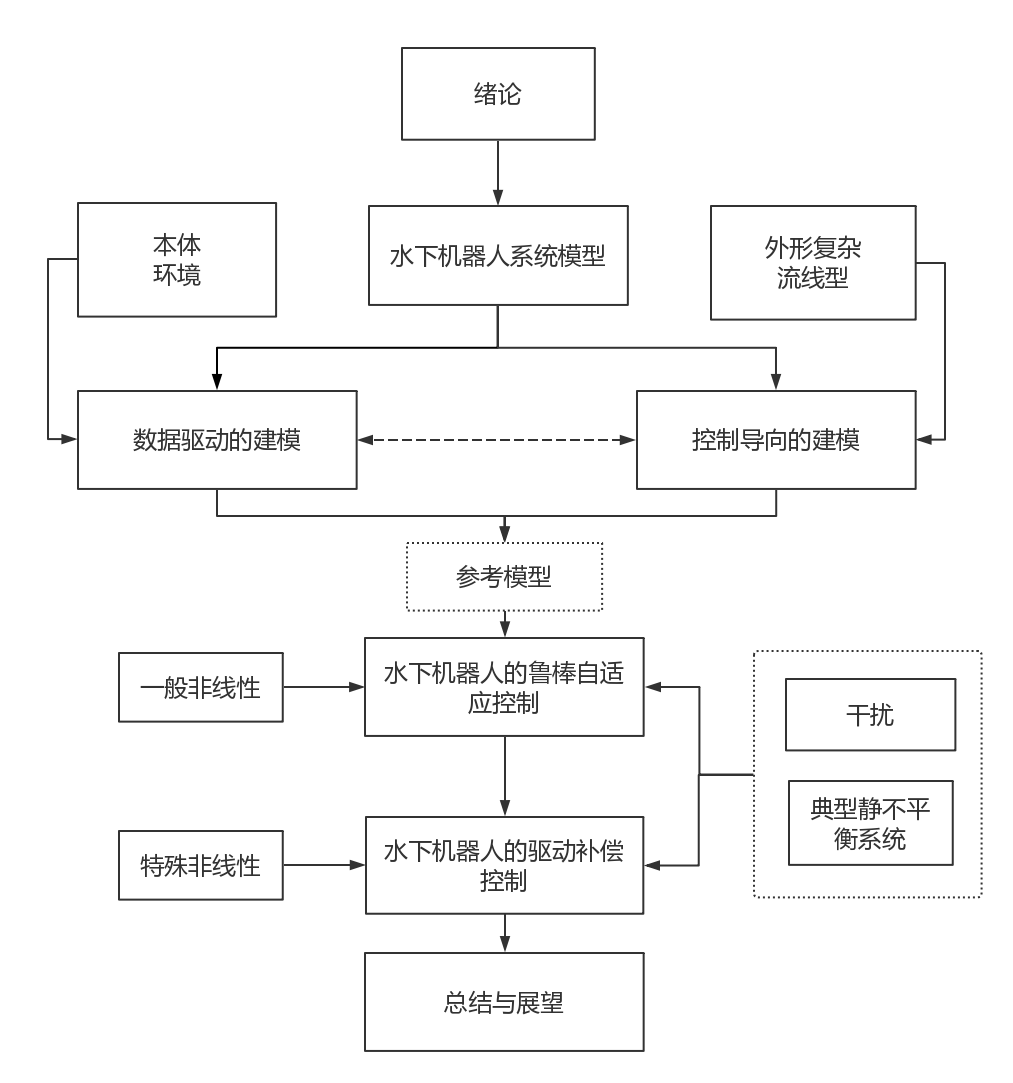
\includegraphics[width=14cm]{figure/chap1/diagram_2.png}
%\captionsetup{justification=centering}
\label{fig:chap1:F4}
\bicaption[fig:chap1:F4]{论文研究路线图}{论文研究路线图}{Fig.}{Diagram for this thesis}
\end{figure*}


\subsection{本文的研究路线图 }

% 水下机器人: ROV 外形复杂 AUV 流线型与鱼雷相类

% 系统建模 : 运动学动力学建模:驱动类型、推力分配与控制、 数据驱动建模:参数辨识、结构搜索、 环境建模:侧线原理、机器学习

% 控制应用的建模: 数值建模: 关键项:阻尼、附加质量   经验法、 数值计算法、 泰勒展开处理

% 控制 : 鲁棒性、 自适应性、 一般非线性、 特殊非线性、死区、延迟、阈值 现代补偿器、 基于Riccati方程的补偿器
本文的研究从水下机器人的系统分析展开,层层推进,进而实现研究目标。全文的研究路线如下所图\ref{fig:chap1:F4}所示:







\section{本章小结 }

本章中首先给出了水下机器人建模与非线性自适应控制的研究意义,着重对水下机器人的动力学建模与数据驱动的系统建模、鲁棒自适应控制及补偿优化进行了现状总结,提出围绕水下机器人的启发式建模与非线性问题问题的鲁棒自适应控制展开研究,重点放在水下机器人的数学模型搜索与系统辨识、水下机器人的控制导向的模型构建、鲁棒自适应控制以及驱动补偿控制上,并给出本文的研究路线图。

%# -*- coding:utf-8 -*-
%!TEX root = ../thesis.tex
%%==================================================
%% chapter02.tex for SJTU Master Thesis
%% Encoding: UTF-8
%%==================================================
\newcommand\bu{\bm{u}}
\newcommand\bx{\bm{x}}


%\newcommand{\tabincell}[2]{\begin{tabular}{@{}#1@{}}#2\end{tabular}}


\chapter{水下机器人系统模型 }

% 参考的资料fossen的书\\
%  remus的硕士论文\\
% 欠驱动与全驱动机器人的介绍russ tedrake http://underactuated.csail.mit.edu/underactuated.html

\label{chap:Theory}
% 2.1 引言
% 2.2 运动系统数学描述
% 2.2.1 水下机器人的坐标系统
% 2.2.2 水下机器人的运动动力学模型
% 2.2.3 不同类型的水下机器人模型
% 2.2.3.1 全驱动水下机器人的数学模型
% 2.2.3.2 欠驱动水下机器人的数学模型
% 2.3 推进器布置与推力控制向量
% 2.4 本章小结
\section{引言}
水下机器人可根据设备应用的目标与操控方式的不同通常可以分为自治式水下机器人(AUV)、遥控水下机器人(ROV)。水下机器人的种类不同使得不同的水下机器人在设计开发阶段就着重于不同的水下功用,但这样的划分主要是从功用角度划分,这使得研究者在后续的控制开发中容易忽略动态系统本身的特性,更过多地依赖于控制系统设计。运动学、动力学理论常常被用来分析水下机器人的运动,这种方法无论是AUV还是ROV类型的水下机器人均可使用。水下机器人的运动空间是6自由度的,采用矩阵形式的运动动力学方程可以用于水下机器人的理论分析,但是从现代机器人行业的发展对水下机器人研究带来的挑战的角度,即如何更好利用蕴含在机器人设备中的自然动力学或者系统特性更好地改善控制系统的设计,精确地建立航行器的数学模型代价太高。

根据机器人的控制输入与系统的自由度,机器人控制也会呈现出不同的驱动特性。参考现代机器人(机器鱼、 ASIMO、飞行器)与生物(鱼、鸟类)的在执行任务与获得的运动性能的运动自然性上的强烈差异,机器人(鱼)就像一个不太熟悉自身系统的人(鱼)\cite{russdrakebook}。这是因为过往的机器人控制系统主要采用状态反馈控制的方法,虽然可以让机器人系统追踪上期望轨迹,但是这样的控制不仅需要使用高增益的反馈并耗费较多的能量,还需要设计者对控制理论比较精通。(水下)机器人研究的目标是其实现卓越的动态性能(效率,敏捷性和鲁棒性),这需要研究者意识到利用系统的动态特性来开发控制系统的重要性,而不是消除它们。水下机器人的研究主要就是建立可以利用机器人系统的动力学特性来设计控制系统。

一般而言,根据水下机器人工作的水下空间和推进器的分配布置,水下机器人,尤其是深海工作的无人自治水下机器人,多是控制输入小于系统的自由度。本章为了便于后续的控制建模研究,将水下机器人基于外形划分成为鱼雷型水下机器人和具有复杂外形的水下机器人。两种水下机器人的系统描述都是基于海洋运载器的数学模型,主要从静力学、动力学来描述水下机器人在体坐标系下的力与运动的关系,并通过建立大地坐标系与体坐标系来完成状态量的转换。描述水下机器人的方法有许多种,主要有运动动力学建模法、使用实验数据系统建模法来获取载体系统的数学模型。本章的工作是从利用系统动态和便于模型参数计算的角度对水下机器人进行分类,并演绎水下机器人的运动动力学模型的各个具体形式。结合推进器的空间安装位置,从运动学的角度给出推力分配模型。根据水下机器人运动面的划分,对一般形式的推力分配模型进行演化,但与所要控制的运动而言,有些推进器的布置并不是最合适的。基于控制目标,分析各推进器对每个自由度运动的贡献,提出推力控制向量,以便定义单个推进器对各自由度的力学影响。结合ROV的姿态控制,将PID控制器与推力控制向量结合,以优化推力的分配,改善控制性能。

\section{运动系统数学描述 }

水下机器人系统的数学建模涉及到运动学、动力学、静力学的有关知识。运动学是涉及水下机器人的有关量表达以及运动转换的几何方面研究。静力学主要关于水下机器人处于静止或者稳定状态的力学平衡,动力学主要是与本体有关加速运动的力学分析。本部分首先介绍水下机器人的六个自由度的运动学动力学模型以及关键项,分别建立水下机器人的刚体平动、转动的模型以及非线性航行器模型。为了便于引入后续的系统辨识和模型计算章节,重点介绍两种不同机器人的数学模型。

\begin{figure}[!htp]
\centering
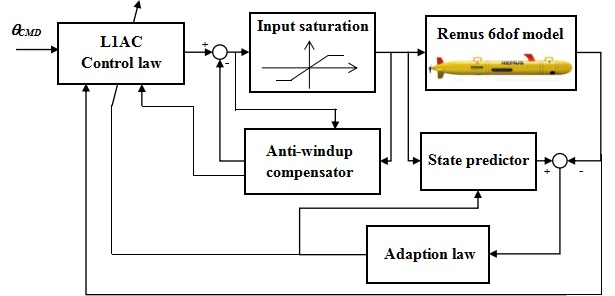
\includegraphics[width=10cm,height=9cm]{figure/chap2/F1.eps}
%\captionsetup{justification=centering}
% \caption{水下运载器坐标示意图}
% \label{paper_f11}
\label{fig:chap2:F1}
\bicaption[fig:chap2:F1]{水下运载器坐标示意图}{水下运载器坐标示意图} {Fig.}{Underwater vehicle frames}
\end{figure}

\begin{table}[!hpb]
\centering
\label{tab:chap2:notation}
\bicaption[tab:chap2:notation]{水下机器人符号量示意}{水下机器人符号量示意}{Table}{ Notations for Underwater vehicle\cite{fossen1994guidance}}
\begin{tabular}{cccc}
\toprule
      & Position \& Angles   &  Linear \& Angular Velocities  & Forces \& Moments \\
Coordinate & E-frame & B-frame & B-frame \\ \midrule
Surge & $X$      &  $u$ & $F_X$ \\
Sway  & $Y$      &  $v$ & $F_Y$ \\
Heave & $Z$      &  $w$ & $F_Z$ \\
Roll  & $\varphi$&  $p$ & $M_K$ \\
Pitch & $\theta$ &  $q$ & $M_M$ \\
Yaw   & $\psi$   &  $r$ & $M_N$ \\
\bottomrule
\end{tabular}
\end{table}

\subsection{水下机器人的运动学 }

在水下机器人中,通常会采用两个坐标系来描述水下机器人本体的运动,即载体坐标系(B-frame)和惯性坐标系(E-frame),如图所示\ref{fig:chap2:F1}。其中,载体坐标系统(B-frame)的坐标原点$O$位于水下机器人本体的几何中心上,载体坐标系的x轴的正向为水下机器人的前进方向,载体坐标系的y轴指向水下机器人的右侧,载体坐标系的定义符合右手定义,因此z轴指向水下机器人的正下方。惯性坐标系(E-frame),也常被称为大地坐标系,大地坐标系的定义可以参考海军建筑师和船舶工程师学会(SNAME)在1950年建立的坐标系规范,其中大地坐标系常被用来描述水下机器人的运动任务以及导航位置,该坐标系的X、Y、Z分别指向北(North)、东(East)、地心(Down),因此大地坐标系也被称为NED-frame\cite{fossen1994guidance}。考虑后面水下机器人建模的复杂性,为了方便,模型是在载体坐标系内建立的,而水下机器人各运动量可以参见表\ref{tab:chap2:notation}。机器人的方位姿态和位置$\bm \eta$是在E-frame内定义,速度量$\bm \nu$是在B-frame中表示的,水下机器人受到的力和力矩$\bm \tau$ 也是在B-frame表示,如公式\ref{eq:chap2:1}。在海洋运载器的导航与控制系统中,运载器的姿态是使用欧拉角(或四元数)来表示的,本章中为了便于后续的使用,也将会介绍载体坐标系运动学方程相对于惯性坐标系的转换关系。在表\ref{tab:chap2:notation}中,水下机器人的六个自由度都被反映并示意出来,Surge是纵荡,Sway是横荡,Heave是垂荡,Roll是横滚,Pitch是俯仰,Yaw是偏航。所有的位置、姿态、线速度、角速度以及力、力矩都分别与这六个自由度对应。



\begin{equation}
\centering
\label{eq:chap2:1}
\begin{aligned}
 {\bm{\eta}}  &= {[X,Y,Z,\varphi ,\theta ,\psi ]^T} \\
 {\bm{\nu}} &= {[u,v,w,p,q,r]^T} \\
 {\bm{\tau}_{RB}} &= {[ \sum {F_X}, \sum {F_Y}, \sum {F_Z}, \sum {M_K}, \sum {M_M}, \sum {M_N}]^T}\\
 \end{aligned}
 \end{equation}
 其中,为了便于进行姿态和位置计算,定义如下向量:
 \begin{equation*}
 \centering
 \label{eq:chap2:2}
 \begin{array}{l}
 {{\bm{\eta}} _1} = {[X,Y,Z]^T} \\
 {{\bm{\eta}} _2} = {[\varphi ,\theta ,\psi ]^T}\\
 {{\bm{\nu}} _1}= {[u,v,w]^T}\\
 {{\bm{\nu}} _2}= {[p,q,r]^T}\\
 {{\bm{\tau}}_1} = {[ \sum {F_X}, \sum {F_Y}, \sum {F_Z}]^T}\\
 {{\bm{\tau}}_2} = {[ \sum {M_K}, \sum {M_M}, \sum {M_N}]^T}\\
 \end{array}
 \end{equation*}



平移运动的速度向量在载体坐标系和惯性坐标系的转换如下公式\ref{eq:chap2:3}所示:

\begin{equation}
\centering
\label{eq:chap2:3}
\left[ {\begin{array}{*{20}{c}}
   {\dot X}  \\
   {\dot Y}  \\
   {\dot Z}  \\
\end{array}} \right] =
 {{\bm{J}}_{1}(\bm{\eta}_{2})}
\left[ {\begin{array}{*{20}{c}}
   u  \\
   v  \\
   w  \\
\end{array}} \right]
\end{equation}
其中,
\begin{equation*}
\centering
\label{eq:chap2:4}
{{\bm{J}}_{1}(\bm{\eta} _{2})} =
\left[
{\begin{array}{*{20}{c}}
   {{\mathop{\rm c}\nolimits}  \psi  c \theta  } & { - s \psi  c \varphi   + c \psi  s \varphi  s \theta  } & {s \psi  s \varphi   + {\mathop{\rm c}\nolimits}  \psi  c \varphi  s \theta  }  \\
   {s \psi  c \theta  } & {c \psi  c \varphi   + s \psi  s \varphi  s \theta  } & { - c \psi  s \varphi   + s \psi  c \varphi  s \theta  }  \\
   { - s \theta  } & {c \theta  s \varphi  } & {c \theta  c \varphi  }  \\
\end{array}}
\right]
\end{equation*}
\\
在上述公式以及后面的方程中,为了描述方便,定义 $ c= cos(·)$ ,  $s = sin(·)$, $t = tan(·)$。需要注意的是,${{\bm{J}}_{1}(\bm{\eta} _{2})}$ 是正交矩阵,因此,

\begin{equation}
\label{eq:chap2:5}
({{\bm{J}}_{1}(\bm{\eta} _{2})})^{-1} = ({{\bm{J}}_{1}(\bm{\eta} _{2})})^T
\end{equation}

旋转运动的速度向量在载体坐标系和惯性坐标系的转换如下,如下公式所示\ref{eq:chap2:6}:

\begin{equation}
\label{eq:chap2:6}
\left[ {\begin{array}{*{20}{c}}
   \dot \varphi   \\
   \dot \theta   \\
   \dot \psi   \\
\end{array}} \right] = {\bm{J}_2(\bm{\eta}_2)}
\left[ {\begin{array}{*{20}{c}}
   p  \\
   q  \\
   r  \\
\end{array}} \right]
\end{equation}
其中,${\bm{J}_2(\bm{\eta}_2)}$ 的具体表示如下

\begin{equation*}
\centering
\label{eq:chap2:7}
{\bm{J}_2(\bm{\eta}_2)} =
 \left[ {\begin{array}{*{20}{c}}
   1 & {{\mathop{\rm s}\nolimits}  \varphi  {\mathop{\rm t}\nolimits}  \theta  } & {{\mathop{\rm c}\nolimits}  \varphi  {\mathop{\rm t}\nolimits}  \theta  }  \\
   0 & {{\mathop{\rm c}\nolimits}  \varphi  } & { - {\mathop{\rm s}\nolimits}  \varphi  }  \\
   0 & {{\mathop{\rm s}\nolimits}  \varphi  /{\mathop{\rm c}\nolimits}  \theta  } & {{\mathop{\rm c}\nolimits}  \varphi  /{\mathop{\rm c}\nolimits}  \theta  }  \\
\end{array}} \right]
\end{equation*}

需要注意的是,${\bm{J}_2(\bm{\eta}_2)}$ 的公式并不适用与俯仰角度 $\theta$ 接近+90度或者-90度的情况。 对于水下机器人的运动描述,这个问题并不会影响使用,因为实际的使用水下机器人几乎不会到达这个奇点。如果是需要对极端情况的俯仰角度进行建模研究,也可以使用四元数或者罗德里格斯参数来实现\cite{fossen1994guidance}。

通过使用公式\ref{eq:chap2:3}和\ref{eq:chap2:6}的线速度转换矩阵与旋转变换矩阵,可以得到水下机器人载体坐标系与惯性坐标系之间的运动学关系:

\begin{equation}
\label{eq:chap2:8}
\dot{\bm{\eta}}= \bm{J(\bm{\eta}_2)}   \dot{\bm{\nu}}
\end{equation}

可以发现$\bm{J(\bm{\eta}_2)}$ 是关于 $\bm{\eta}_2$ 的函数,其具体数学描述如下:

\begin{equation}
\label{eq:chap2:9}
\bm{J(\bm{\eta}_2)} = \begin{bmatrix}
 {\bm{J}_1(\bm{\eta}_2)}  &   \bm{0}_{3 \times 3}\\
 \bm{0}_{3 \times 3}      &  {\bm{J}_2(\bm{\eta}_2)}
\end{bmatrix}
\end{equation}

通过使用上面的运动学定义与相关量的转换,可以继续水下机器人的动力学建模工作。

\subsection{水下机器人的动力学模型  }
由于航行器所受到刚体动力学与流体动力学作用到本体上具有同时性,可以根据线性系统的等效叠加原理进行动力学建模\cite{lamb1932hydrodynamics}。因此,将水下机器人的动力学建模主要分为刚体动力学建模与流体动力学建模。

\subsubsection{航行器的刚体动力学 }

在本部分进行的刚体动力学的研究是不考虑水对运载器的影响,且在载体坐标系上使用牛顿定律、欧拉运动定律进行分析。因此,需建立两个假设:一是水下机器人被假设为一个理想的刚体,其受到的所有力学作用等效为一个合外力(矩);二是认为定义在地球上的惯性坐标系不受地球运动产生的力影响\cite{prestero2001verification}。刚体动力学的研究也是从平动和旋转运动两个方面展开。

在进行研究前,需要定义水下机器人在载体坐标系的重心和浮心的位置,如下所示:
\begin{equation}
\label{eq:chap2:10}
\begin{aligned}
{\bm{r}}_{G} &= [ x_G,  y_G,  z_G ]^T  \\
{\bm{r}}_{B} &= [ x_B,  y_B,  z_B ]^T  \\
\end{aligned}
\end{equation}

考虑到体坐标系的原点不位于水下机器人的几何中心上,具有一般性。因此水下航行器的6自由度的刚体动力学方程如下:
\begin{equation}
\label{eq:chap2:11}
 %\begin{array}{l}
 \begin{aligned}
 m\left[ {\dot u - vr + wq - {x_G}({q^2} + {r^2}) + {y_G}(pq - \dot r) + {z_G}(pr + \dot q)} \right] &= \sum {{F_X}}  \\
 m\left[ {\dot v - wp + ur - {y_G}({r^2} + {p^2}) + {z_G}(qr - \dot p) + {x_G}(qp + \dot r)} \right] &= \sum {{F_Y}}  \\
 m\left[ {\dot w - uq + vp - {z_G}({q^2} + {p^2}) + {x_G}(rp - \dot q) + {y_G}(rq + \dot p)} \right] &= \sum {{F_Z}}  \\
 {I_x}\dot p + ({I_z} - {I_y})qr -(\dot r + pq)I_{xz}+(r^2-q^2)I_{yz}+(pr-\dot q)I_{xy}\\
               + m[{y_G}(\dot w - uq + vp) - {z_G}(\dot v - wp + ur)] &= \sum {{M_K}}  \\
 {I_y}\dot q + ({I_x} - {I_z})rp -(\dot p + qr)I_{xy}+(p^2-r^2)I_{xz}+(qp-\dot r)I_{yz}\\
               + m[{z_G}(\dot u - vr + wq) - {x_G}(\dot w - uq + vp)] &= \sum {{M_M}}  \\
 {I_z}\dot r + ({I_y} - {I_x})pq -(\dot q + rp)I_{yz}+(q^2-p^2)I_{xy}+(rq-\dot p)I_{xz}\\
               + m[{x_G}(\dot v - wp + ur) - {y_G}(\dot u - vr + qw)] &= \sum {{M_N}}  \\
 \end{aligned}
 %\end{array}
 \end{equation}
式\ref{eq:chap2:11}中$m$ 是水下机器人的质量,公式的前三个方程表示平移运动,后三个方程表示旋转运动。

将上述方程表达成更加紧凑的矩阵形式:

\begin{equation}
\label{eq:chap2:12}
\bm{M_{RB}} {\dot{\bm{\nu}}} + \bm{C_{RB}}(\bm{\nu}){\bm{\nu}} =  {\bm{\tau}_{RB}}
\end{equation}
公式\ref{eq:chap2:12}即是水下机器人的刚体动力学的一般形式,其中${\bm{\tau}_{RB}}$是外部的力、力矩的合向量。刚体惯性质量矩阵是唯一不随时间变化的,并且具有如下属性:$\bm{M_{RB}} = \bm{M_{RB}}^T > \bm{0}$。$\bm{M_{RB}}$的具体表达见公式\ref{eq:chap2:13}, $\bm{\tau_{RB}}$ 在公式\ref{eq:chap2:1}已经被定义。
\begin{equation}
\label{eq:chap2:13}
\begin{aligned}
\bm{M_{RB}} &= \begin{bmatrix}
               {m {\bm{I_{3 \times 3}} }} & {-m {\bm{S_{r_G}} } }   \\
                 m {\bm{S_{r_G}} }         &  \bm{I_0} \\
               \end{bmatrix}
            &= \begin{bmatrix}
                   m & 0       &  0    & 0        & m z_G   & -m y_G     \\
                   0 & m       &  0    & -m z_G   & 0       & m x_G      \\
                   0 & 0       &  m    &  m y_G   & -m x_G  & 0          \\
                   0 &  -m z_G & m y_G &  I_x     & -I_{xy} & -I_{xz}    \\
               m z_G &   0     & -m x_G& -I_{yx}  & I_y     & -I_{yz}    \\
              -m y_G &  m x_G  &  0    & -I_{zx}  & -I_{zy} & I_z        \\
               \end{bmatrix}
\end{aligned}
\end{equation}
式\ref{eq:chap2:13}中,${\bm{I_{3 \times 3}}}$为单位矩阵,$\bm{I_0}$ 是惯性张量矩阵,$\bm{S_{r_G}}$是斜对称矩阵。

式\ref{eq:chap2:12}中, ${\bm{C_{RB}}(\bm{\nu})}$ 是科氏力-离心力矩阵,  它包括科氏力向量项与离心力向量项, 是斜对称矩阵, 也具有如下性质:${\bm{C_{RB}}(\bm{\nu})}= - {\bm{C_{RB}}(\bm{\nu})}^T$,具体可参考附录定理\ref{app_A:thm:1}的惯性矩阵的科氏力-离心力矩阵参数化定理。

${\bm{C_{RB}}(\bm{\nu})}$ 的具体定义参数化如下:
% \begin{equation}
% \bm{C_{RB}}(\bm{\nu}) {\buildrel \Delta \over =}
% \begin{bmatrix}
% 0 & 0 & 0  & m(y_G q + z_G r) & -m(x_G q - w)   & -m(x_G r + v)   \\
% 0 & 0 & 0  & -m(y_G p +w)     & m(z_G r +x_G p) & -m(y_G r - u)  \\
% 0 & 0 & 0  & -m(z_G p - v)    & -m(z_G q + u)   & m(x_G p + y_G q)  \\
% -m(y_G q + z_G r) & m(y_G p+w)   & m(z_G p - v) &0  & -I_{yz}q-I_{xz}p+I_z r &  I_{yz}r +I_{xy}p - I_y q          \\
% m(x_G q - w) & -m(z_G r + x_G p)  &  m(z_G q+u) & I_{yz}q+I_{xz}p - I_z r & 0 & -I_{xz}r - I_{xy}q + I_{x}p \\
% m(x_G r + v) &  m(y_G r - u) & -m(x_G p + y_G q) & -I_y r - I_{xy}p +I_y q & I_{xz}r+I_{xy}q-I_x p &  0 \\
% \end{bmatrix}
% \end{equation}
\begin{multline}
\label{eq:chap2:14}
%\begin{aligned}
\bm{C_{RB}}(\bm{\nu})
{\buildrel \Delta \over =}
% \begin{bmatrix}
%   0 & 0  \\
%   0 & 0  \\
% \end{bmatrix}\\
% =
  \left[\begin{array}{ccc}
0 & 0 & 0 \\
0 & 0 & 0 \\
0 & 0 & 0 \\
-m(y_G q + z_G r) & m(y_G p+w)   & m(z_G p - v) \\
m(x_G q - w) & -m(z_G r + x_G p)  &  m(z_G q+u) \\
m(x_G r + v) &  m(y_G r - u) & -m(x_G p + y_G q) \\
\end{array}\right.\\
\left.\begin{array}{ccc}
  m(y_G q + z_G r) & -m(x_G q - w)   & -m(x_G r + v)   \\
  -m(y_G p +w)     & m(z_G r +x_G p) & -m(y_G r - u)  \\
 -m(z_G p - v)    & -m(z_G q + u)   & m(x_G p + y_G q)  \\
 0  & -I_{yz}q-I_{xz}p+I_z r &  I_{yz}r +I_{xy}p - I_y q   \\
 I_{yz}q+I_{xz}p - I_z r & 0 & -I_{xz}r - I_{xy}q + I_{x}p \\
 -I_y r - I_{xy}p +I_y q & I_{xz}r+I_{xy}q-I_x p &  0 \\
\end{array}\right]
%\end{aligned}
\end{multline}

因此,可以获得水下机器人的矩阵形式刚体动力学,并对各项进行参数化分析。

考虑前面的体坐标系的原点不是位于水下机器人的几何中心上,假设浮心与载体坐标系原点重合,则可以获得对角化的惯性张量矩阵:

\begin{equation}
\label{eq:chap2:15}
\bm{I}_0 = \begin{bmatrix}
 I_x  & 0    &  0   \\
 0    & I_y  &  0   \\
 0    & 0    &  I_z \\
\end{bmatrix}
\end{equation}

简化后的运动方程如下:
\begin{equation}
\centering
\label{eq:chap2:16}
\begin{array}{l}
 m\left[ {\dot u - vr + wq - {x_G}({q^2} + {r^2}) + {y_G}(pq - \dot r) + {z_G}(pr + \dot q)} \right] = \sum {{F_X}}  \\
 m\left[ {\dot v - wp + ur - {y_G}({r^2} + {p^2}) + {z_G}(qr - \dot p) + {x_G}(qp + \dot r)} \right] = \sum {{F_Y}}  \\
 m\left[ {\dot w - uq + vp - {z_G}({q^2} + {p^2}) + {x_G}(rp - \dot q) + {y_G}(rq + \dot p)} \right] = \sum {{F_Z}}  \\
 {I_x}\dot p + ({I_z} - {I_y})qr + m[{y_G}(\dot w - uq + vp) - {z_G}(\dot v - wp + ur)] = \sum {{M_K}}  \\
 {I_y}\dot q + ({I_x} - {I_z})rp + m[{z_G}(\dot u - vr + wq) - {x_G}(\dot w - uq + vp)] = \sum {{M_M}}  \\
 {I_z}\dot r + ({I_y} - {I_x})pq + m[{x_G}(\dot v - wp + ur) - {y_G}(\dot u - vr + qw)] = \sum {{M_N}}  \\
 \end{array}
 \end{equation}

\subsubsection{航行器作用力 }

本部分主要从水下机器人的流体力学角度对运载器进行分析,根据刚体动力学模型公式\ref{eq:chap2:12}右侧表示的作用于水下机器人上的外部合力与力矩以及线性叠加原理,合力(矩)的产生原因可以分为如下几类:
一. 流体作用力$\bm{\tau}_{H}$,包括附加质量、流体阻尼力、恢复力(浮力与重力共同作用的静力学分析)。二. 环境干扰力$\bm{\tau}_E$,一般因受到海流、风、波浪环境影响而产生,由于水下机器人所工作的环境主要在深水区域, 因此本章仅考虑海流的力学效应。另外,在水下机器人中水流对水下机器人的影响被视为干扰力,一般通过控制来克制,不过本文对于水流的研究不仅仅处于将水流视为外界的干扰,也在主动地识别流体的特性,主动利用水下环境。在第三章中,会给出关于水流的特性识别的有关研究工作。三. 驱动力$\bm{\tau}$,一般包括推进器、舵片的力学作用。

根据水下机器人受到的外部力(矩)的成因,给出作用力的数学描述如下:
\begin{equation}
\centering
\label{eq:chap2:17}
\bm{\tau}_{RB} = \bm{\tau}_{H} + \bm{\tau}_E +  \bm{\tau}
\end{equation}
\begin{equation}
\label{eq:chap2:18}
\bm{\tau}_{H} = -{\bm{M}_A}{\bm{\dot \nu}} - {\bm{C}_A}(\bm{\nu}) {\bm{\nu}} - \bm{D}(\bm{\nu})\bm{\nu}-\bm{g}({\bm{\eta}})
\end{equation}
式\ref{eq:chap2:17}与式\ref{eq:chap2:18} 共同给出水下航行器受到的外部作用力和力矩的数学模型。

为了便于进行水下机器人建模与控制应用,下面分别给出相关项的参数化矩阵与数学分析。

A. 附加质量项

惯性附加质量$\bm{M}_A$ 是由水下机器人在水中加速运动而产生的水动力。 对于完全没入水中的水下机器人, 在对附加质量$\bm{M}_A $求解时会假设附加质量的系数是恒定不变的,并且不受波浪频率的影响,但是附加质量的某些项却比机器人的本体质量大很多。基于这个假设,流体动能来被用来分析附加质量项,当水下机器人在水中加速运动时,机器人头部的流体会因前进运动而向机器人后方移动,这样的移动必定会耗费的能量。附加质量项定义如下:

\begin{equation}
\centering
\label{eq:chap2:19}
\begin{aligned}
\bm{M}_{A}  &= \begin{bmatrix}
                 \bm{A}_{11}   &  \bm{A}_{12}   \\
                 \bm{A}_{21}   &  \bm{A}_{22}   \\
               \end{bmatrix}                    \\
            &=-\begin{bmatrix}
 X_{\dot u} &  X_{\dot v} &  X_{\dot w} &  X_{\dot p} &  X_{\dot q} &  X_{\dot r} \\
 Y_{\dot u} &  Y_{\dot v} &  Y_{\dot w} &  Y_{\dot p} &  Y_{\dot q} &  Y_{\dot r} \\
 Z_{\dot u} &  Z_{\dot v} &  Z_{\dot w} &  Z_{\dot p} &  Z_{\dot q} &  Z_{\dot r} \\
 K_{\dot u} &  K_{\dot v} &  K_{\dot w} &  K_{\dot p} &  K_{\dot q} &  K_{\dot r} \\
 M_{\dot u} &  M_{\dot v} &  M_{\dot w} &  M_{\dot p} &  M_{\dot q} &  M_{\dot r} \\
 N_{\dot u} &  N_{\dot v} &  N_{\dot w} &  N_{\dot p} &  N_{\dot q} &  N_{\dot r} \\
              \end{bmatrix}
\end{aligned}
\end{equation}
式中,$\bm{A}_{11}$, $ \bm{A}_{12}$, $\bm{A}_{21}$,$\bm{A}_{22}$均为$3 \times 3$矩阵,其余量为水下机器人的与加速度有关的流体动力学参数。

由于附加质量$\bm{M}_A$ 产生的科氏力-离心力, 水下机器人在做旋转运动的时候也会因加速而消耗能量。 因此,给出斜对称矩阵${\bm{C}_A}\left( \bm{ \nu}  \right)$的定义:
\begin{equation}
\centering
\label{eq:chap2:20}
{\bm{C}_A}\left( \bm{ \nu}  \right) = \left[ {\begin{array}{*{20}{c}}
   0 & 0 & 0 & 0 & { - {a_3}} & {{a_2}}  \\
   0 & 0 & 0 & {{a_3}} & 0 & { - {a_1}}  \\
   0 & 0 & 0 & { - {a_2}} & {{a_1}} & 0  \\
   0 & { - {a_3}} & {{a_2}} & 0 & { - {b_3}} & {{b_2}}  \\
   {{a_3}} & 0 & { - {a_1}} & {{b_3}} & 0 & { - {b_1}}  \\
   { - {a_2}} & {{a_1}} & 0 & { - {b_2}} & {b1} & 0  \\
\end{array}} \right]
\end{equation}

其中,\begin{equation*}
\label{eq:chap2:21}
\begin{array}{l}
 {a_1} = {X_{\dot u}}u + {X_{\dot v}}v + {X_{\dot w}}w + {X_{\dot p}}p + {X_{\dot q}}q + {X_{\dot r}}r \\
 {a_2} = {X_{\dot v}}u + {Y_{\dot v}}v + {Y_{\dot w}}w + {Y_{\dot p}}p + {Y_{\dot q}}q + {Y_{\dot r}}r \\
 {a_3} = {X_{\dot w}}u + {Y_{\dot w}}v + {Z_{\dot w}}w + {Z_{\dot p}}p + {Z_{\dot q}}q + {Z_{\dot r}}r \\
 {b_1} = {X_{\dot p}}u + {Y_{\dot p}}v + {Z_{\dot p}}w + {K_{\dot p}}p + {K_{\dot q}}q + {K_{\dot r}}r \\
 {b_2} = {X_{\dot p}}u + {Y_{\dot q}}v + {Z_{\dot q}}w + {K_{\dot q}}p + {M_{\dot q}}q + {M_{\dot r}}r \\
 {b_3} = {X_{\dot r}}u + {Y_{\dot r}}v + {Z_{\dot r}}w + {K_{\dot r}}p + {M_{\dot r}}q + {N_{\dot r}}r \\
 \end{array}
 \end{equation*}

一般而言,6自由度的水下机器人在水下高速航行是具有强非线性且复杂耦合性。然而,在许多水下机器人中,例如ROV,如果其运动的速度较低,且拥有三个对称平面,这时就可以忽略附加质量项矩阵内不在对角线上的元素。故惯性附加质量矩阵$\bm{M}_A$和$\bm{C}_A$可以简化成如下形式:
\begin{equation}
\centering
\label{eq:chap2:22}
\bm{M}_A = -diag\{X_{\dot u},Y_{\dot v},Z_{\dot w},K_{\dot p},M_{\dot q},N_{\dot r}\}
\end{equation}
\begin{equation}
\label{eq:chap2:23}
\centering
\bm{C}_A  = \begin{bmatrix}
 0           &0            &0               &0                  &-Z_{\dot w} w   & Y_{\dot v} v\\
 0           &0            &0               &Z_{\dot w}w        &0               &-X_{\dot u}u\\
 0           &0            &0               &-Y_{\dot v}v       & X_{\dot u} u   &   0    \\
 0           & -Z_{\dot w}w & Y_{\dot v}v   &  0                & -N_{\dot r}r   & M_{\dot q}q\\
 Z_{\dot w}w &0            &-X_{\dot u}u    & N_{\dot r}r       & 0              &-K_{\dot p}p \\
 -Y_{\dot v}v& X_{\dot u}u &0               &-M_{\dot q}q       & K_{\dot p}p    & 0\\
\end{bmatrix}
\end{equation}
虽然获得的附加质量矩阵是简化的,但在实际使用是,这种近似方法的估计效果良好,这是因为对角线上的元素远大于非对线上的元素。对于超小型的水下机器人,因本体质量较小,且速度足够小,一般可以将$\bm{C}_A$忽略。


B. 阻尼项

公式\ref{eq:chap2:18}中的流体阻尼项的出现主要原因有本体运动而带来的势流阻尼;有机器人本体的表面因运动而产生摩擦阻尼,该阻尼主要与表面积有关;有水下机器人运功因为兴波耗费能量而产生的阻尼;有因流体流过机器人时会产生漩涡而引起机器人的振动而耗散能量的阻尼。总流体动力学阻尼矩阵可以写成这些分量的总和:
\begin{equation}
\label{eq:chap2:24}
\bm{D}({\bm{\nu}})  {\buildrel \Delta \over =} \bm{D}_P(\bm{\nu})+\bm{D}_S(\bm{\nu})+\bm{D}_W(\bm{\nu})+\bm{D}_M(\bm{\nu})
\end{equation}
式中,$\bm{D}_P(\bm{\nu})$ 是势流阻尼项,$\bm{D}_S(\bm{\nu})$是摩擦阻尼项, $\bm{D}_W(\bm{\nu})$是兴波阻尼,$\bm{D}_M(\bm{\nu})$ 是漩涡脱落阻尼。

在水下机器人中,$\bm{D}_P(\bm{\nu})$相比于别的耗散项如粘性阻尼都是可以忽略的。

考虑运载器的运动是低频的,层流边界层产生的线性表皮摩擦会很重要。另外由于线性摩擦对于湍流边界层也有影响,因此通常认为$\bm{D}_W(\bm{\nu})$ 是重要的,且是二次非线性表皮摩擦。

水下机器人多工作于深海,而在靠近海表面运动才会有$\bm{D}_M(\bm{\nu})$产生。因此,在水下机器人中一般会忽略 兴波阻尼。

水是粘性流体,因此由于摩擦力的存在这样的系统能量不会保持。漩涡脱落阻尼常采用莫里森公式来计算,而且在经验计算中莫里森公式常被用来计算水下机器人的流体阻尼:
\begin{equation}
\label{eq:chap2:25}
f(U)=-\frac{1}{2} \rho C_{D}(R_n)A \left |U \right | U
\end{equation}
式中,$U$ 是机器人的前进速度;$A$ 是运动方向的投影截面面积;$C_{D}(R_n)$ 是阻力系数;$\rho$是流体密度,一般流体为水。阻尼系数是和雷诺数有关的$R_n$,雷诺数的计算可以参考\cite{fossen1994guidance}。

一般而言,水下机器人的高速6自由度的运动是强非线性的和耦合的。然而,假如水下机器人有三个对称面,可以做一个线性近似,这样二阶及以上的项就可以忽略。这表明$\bm{D}(\bm{\nu})$的对角线上只有线性的和二次阻尼项。 公式如下:
\begin{equation}
\label{eq:chap2:26}
\begin{aligned}
\bm{D}(\bm{\nu})= &- diag\{ X_u,Y_v,Z_w,K_p,M_q,N_r\}   \\
                  &- diag\{ X_{u\left|u\right|} \left|u\right|, Y_{v\left|v\right|} \left|v\right| , Z_{w\left|w\right|} \left|w\right|, K_{p\left|p\right|} \left|p\right| , M_{q \left| q \right|} \left| q \right|, N_{r \left| r \right|} \left| r \right|  \}
\end{aligned}
\end{equation}
即水下机器人的阻尼项的计算可以总结为线性阻尼和非线性阻尼,其中,非线性的成分会占比更大。

C. 恢复力和力矩

水下机器人中,重力和浮力统称为恢复力。重力的作用点在水下机器人的重心上$\bm{r}_G$ 上, 而浮力的作用点在浮心$\bm{r}_B$ 上。一般而言,水下机器人的重心和浮心是不重合的,并且水下机器人由于在水中的姿态是不断变化的,这样,由于浮力和重力产生力矩也是不断变化的。使用欧拉角在惯性坐标系下给出恢复力和力矩的数学公式:
\begin{equation}
\centering
\label{eq:chap2:27}
\bm{g}(\bm {\eta} ) = \left[ {\begin{array}{*{20}{c}}
   {\left( {W - B} \right)s\theta }  \\
   { - \left( {W - B} \right)c\theta s\varphi }  \\
   { - \left( {W - B} \right)c\theta c\varphi }  \\
   { - \left( {{y_G}W - {y_G}B} \right)c\theta c\varphi  + \left( {{z_G}W - {z_B}B} \right)c\theta s\varphi }  \\
   {\left( {{z_G}W - {z_B}B} \right)s\varphi  + \left( {{x_G}W - {x_B}B} \right)c\theta c\varphi }  \\
   { - \left( {{x_G}W - {x_B}B} \right)c\theta s\varphi  - \left( {{y_G}W - {y_B}B} \right)s\theta }  \\
\end{array}} \right]
\end{equation}
式中,$W$是水下机器人的重力,$B$是浮力。水下机器人中浮力与重力配置会因为水下机器人的类型不同而有所差异,一般ROV中会采用中性浮力,即$W=B$,如BLUEROV。在AUV中,如REMUS-100 AUV中的重力会略小于浮力,这样会使得水下机器人在水里是非稳态系统。这给水下机器人的控制带来了一定的困难。另外,为了减少水下机器人在水里的能量消耗,在设计时也会有重力大于浮力的情况,这种机器人称为重潜于水型水下机器人,多为水下无人机或者水下滑翔机。

D. 驱动器模型

水下机器人的驱动器类型大都是基于流体力学的而设计的,常用的驱动器一般有推进器、控制舵片。水下机器人的驱动器产生力和力矩与水下机器人的固定位置有关,并且驱动器对于水下机器人的各个自由度的影响度也各不相同,将在后面的推力布置部分进行详细讨论。

D.1 螺旋桨模型

对于水下机器人的推进器这种形式,既要描述推进器的布置形式,也要描述单个推进器的数学模型,本部分内容以螺旋桨的推力模型为主。推进器的模型是非线性的,它与水下机器人的航行速度和推进器的转速都有关。为了描述推进器螺旋桨航速和转速的共同作用,给出的推进器的模型如下:
\begin{eqnarray}
\label{eq:chap2:28}
T&=& \rho D^4 K_T (J_0)\|n\| n \\
J_0 &=& \frac{V_a}{nD}\\
K_T&=&\alpha_1 + \alpha_2 \frac{V_a}{nd}
\end{eqnarray}
式中,$K_T$ 是推力系数,$J_0$是流速影响系数。

在ROV中,推进器的推力一般是通过进行敞水实验测定,航向前进速度常被定义为零。推进器的测试台的上配置使用多是S型拉压传感器来测定推进器的正反推力如图\ref{fig:chap2:F2}。推进器也会产生扭矩,在ROV中,推进器一般是成对布置,并且正向推进时的,叶片旋转方向相反,从而抵消推进器的扭矩。因此,推进器的模型就简化成二次非线性表达形式:

\begin{equation}
\label{eq:chap2:29}
T = \alpha_T \left|n\right| n
\end{equation}
式中,$\alpha_T$为敞水推力系数。

\begin{figure}
\label{fig:chap2:F2}
\centering
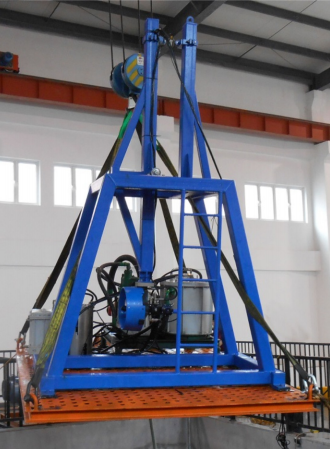
\includegraphics[width = 6cm]{figure/chap2/propellerTest.png}
\bicaption[fig:chap2:F2]{推进器测试台}{推进器测试台}{Fig.}{Test platform for propeller\cite{Huo2016Impulse}}
\end{figure}
本部分建立的推进器螺旋桨的模型描述的是推进器的转速与推力间的关系,但实际中使用的推进器根据推进器采用的驱动方案的不同,推进器的控制输入也不是转速的。液压马达推进器有定量马达和变量马达,电动推进器有无刷直流电机驱动、也有有刷直流电机驱动的方案。因此在实际的应用中可以采用参数辨识方法来确定驱动控制信号与实际推力的关系与系数\cite{wu2016parametric}。

D.2 控制面舵片

安装有控制面舵片的机器人,当航行器在水中前进时,如果舵片与前进方向之间有攻角,舵片上下面会有压力差,产生上升或下降力矩。舵片产生的力矩是水下机器人本体与舵片的共同作用,具有强耦合性与非线性。在确定舵片的力学模型时,一般是采用经验法,与鱼雷数据相对比\cite{bottaccini1954stablity,John1978Methods,Borst1985Fluid}。 另外, 也可以使用实际水下机器人的运行数据来辨识舵片的力学模型,如Hoerner估计方法\cite{Borst1985Fluid}。在后面的水下机器人中使用的舵片就是基于此法建立的模型。

\subsubsection{6自由度水下机器人模型 }

本研究采用的水下机器人的模型是由Fossen提出的非线性海洋运载器模型,该模型是在载体坐标系B-frame下将刚体动力学模型公式\ref{eq:chap2:12}与外部合力和力矩模型公式\ref{eq:chap2:17}合并,并结合运动学方程公式\ref{eq:chap2:8}得到水下机器人的模型公式如下\cite{fossen1994guidance}:
\begin{equation}
\label{eq:chap2:30}
\begin{aligned}
\bm{M} \dot {\bm{\nu}} + \bm{C}(\bm{\nu}) \bm{\nu}&
+ \bm{D}(\bm{\nu}) \bm{\nu} + \bm{g}(\bm{\eta}) = \bm{\tau}_E +  \bm{\tau}\\
&\dot{\bm{\eta}}= \bm{J(\bm{\eta}_2)}   \dot{\bm{\nu}}
\end{aligned}
\end{equation}
式中,$\bm{M} = \bm{M}_{RB} +\bm{M}_A$ ; $\quad \bm{C}(\bm{\nu}) =  \bm{C}_{RB}(\bm{\nu}) +  \bm{C}_{A}(\bm{\nu})$。$\bm{M}_A $ 是水下机器人在水中加速而产生附加质量。$\bm{C}_{A}(\bm{\nu})$ 是由于科氏力-离心力作用产生的附加质量。$\bm{D}(\bm{\nu})$ 是阻尼矩阵。$\bm{g}(\bm{\eta})$ 是恢复力与力矩。

假设$\bm{J}(\bm{\eta})$是非奇异矩阵,那么可以获得水下机器人在惯性坐标系下的运动学模型:
\begin{equation}
\label{eq:chap2:31}
\bm{M}_{\bm{\eta}}{\ddot {\bm{\eta}}} +\bm{C}_{\bm{\eta}}(\bm{\nu},\bm{\eta}) {\dot {\bm{\eta}}} + \bm{D}_{\bm{\eta}} (\bm{\nu},\bm{\eta}) {\dot {\bm{\eta}} }+\bm{g}_{\bm{\eta}}(\bm{\eta}) = \bm{\tau}_{\bm{\eta}}+\bm{\tau}_{\bm{\eta}E}
\end{equation}
式中,
\begin{eqnarray}
\label{eq:chap2:32}
\bm{M}_{\bm{\eta}} &=& \bm{J}^{-T}(\bm{\eta})\bm{M}\bm{J}^{-1}(\bm{\eta})\\
\bm{C}_{\bm{\eta}}(\bm{\nu},\bm{\eta}) &=& \bm{J}^{-T}(\bm{\eta})[\bm{C}(\bm{\nu})-\bm{M}\bm{J}^{-1}(\bm{\eta})\bm{J}(\bm{\eta})] \bm{J}^{-1}(\bm{\eta})\\
\bm{D}_{\bm{\eta}} (\bm{\nu},\bm{\eta})&=& \bm{J}^{-T}(\bm{\eta})\bm{D}\bm{J}^{-1}(\bm{\eta})  \\
\bm{g}_{\bm{\eta}}(\bm{\eta}) &=& \bm{J}^{-T}(\bm{\eta}) \bm{g}(\bm{\eta})  \\
\bm{\tau}_{\bm{\eta}} &=& \bm{J}^{-T}(\bm{\eta}) \bm{\tau}\\
\bm{\tau}_{\bm{\eta}E} &=& \bm{J}^{-T}(\bm{\eta})\bm{\tau}_{E}
\end{eqnarray}


\subsection{不同类型的水下机器人模型 }

水下机器人在不同的状态时,系统就会呈现出不同的动力学特性。在本章中,对水下机器人进行的系统描述是水下机器人完全处于水中,且在水中不受外力干扰。根据水下机器人的外形不同,且为便于水下机器人进行模型参数计算时能够提出一套系统的方法,下面主要对具有非初等几何外形的水下机器人和具有鱼雷外形的水下机器人进行系统描述。

\begin{figure}
\centering
\includegraphics[width=12cm,height=12cm]{figure/chap2/F6.eps}
%\captionsetup{justification=centering}
\label{fig:chap2:F3}
\bicaption[fig:chap2:F3]{水池试验图}{水池试验图}{Fig.}{Way-points tracking experiments in the water}
\end{figure}

\begin{figure}
\centering
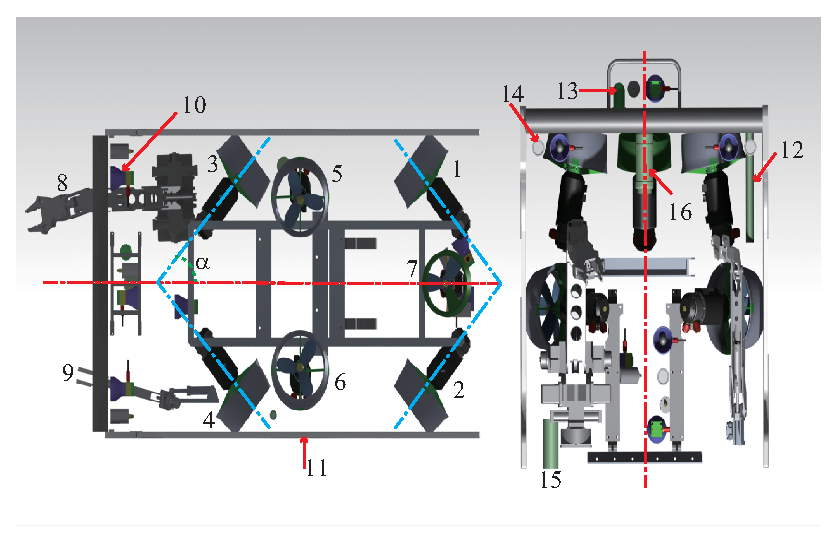
\includegraphics{figure/chap2/F2.eps}
%\captionsetup{justification=centering}
\label{fig:chap2:F4}
\bicaption[fig:chap2:F4]{ROV的分配布置标识图}{ROV的分配布置标识图}{Fig.}{Layout for components of ROV, where 1-7 indicate the position of propellers; 8 and 9 are manipulators used; 10 denotes underwater light; 11 stands for the main frame of vehicle;  12 signifies the wireless beacon of USBL; 13 stands for signal light; 14 is underwater camera;  15 represents the altimeter; 16 expresses the ADCP}
\end{figure}

\begin{table}[h]
\centering
\label{T2:chap2}
\bicaption[T2:chap2]{3000m ROV 的关键参数}{3000m ROV 的关键参数}{Table}{Critical parameters for 3000m ROV}
\begin{tabular}{cccc}
\toprule
               &Value  &Unit   &Description\\
\midrule
\texttt{L}     &2.48     &m  & Overall length\\
\texttt{W}     &1.4      &m  & Width \\
\texttt{H}     &1.63     &m  & Height \\
\texttt{G}     &1413     &kg & Maximum weight\\
\texttt{P}     &1000     &V  & \tabincell{c}{AC Power supply\\ from workstation}\\
\texttt{D$_{max}$}  &3000 &m  & \tabincell{c}{Maximum depth }\\
\texttt{\emph{u}$_{max}$}&2.5 & m/s & Max velocity\\
\texttt{T}&+120 to —90 & kgf &\tabincell{c}{+120:max forward thrust\\-90:max reverse thrust}\\
\texttt{B$_H$}&\tabincell{c}{X-shape\\ $\alpha$=45} & degree & \tabincell{c}{Horizontal propeller\\ arrangement(Fig.\ref{fig:chap2:F4})}\\
\bottomrule
\end{tabular}
\end{table}


\begin{table*}[h]
\centering
\label{T3:chap2}
%\captionsetup{justification=centering}
\bicaption[T3:chap2]{3000m ROV 的传感器列表}{3000m ROV 的传感器列表}{Table}{Sensor descriptions for 3000m ROV}
%\newcommand{\tabincell}[2]{\begin{tabular}{@{}#1@{}}#2\end{tabular}}
\begin{tabular}{cccc}
\toprule
Name & Type &Description\\
\midrule
\texttt{\tabincell{c}{ADCP} }& \tabincell{c}{WorkHorse Monitor} &\tabincell{c}{Teledyne RD Instruments(TRDI) \\Acoustic Doppler Current Profiler(ADCP)} \\
\texttt{\tabincell{c}{INS}}& MU-PHINS-III &\tabincell{c}{IXSEA Inertial navigation system(INS)}\\
\texttt{\tabincell{c}{Depth sensor}}& MiniIPS &\tabincell{c}{Measure depth of vehicle}\\
\texttt{\tabincell{c}{Altimeter} }& Kongsberg 1007 &\tabincell{c}{Measure the altitude(height) of an object\\ above the seafloor}\\
\texttt{\tabincell{c}{USBL} }& MT861S &\tabincell{c}{Positioning underwater target\\ via wireless acoustic communication}\\
\texttt{\tabincell{c}{Gyroscope} }& AHRS-3000 & \tabincell{c}{ Measure roll angle, pitch angle and heading\\ angle with high-precision} \\
\bottomrule
\end{tabular}
\end{table*}

\begin{figure}[h]
\centering
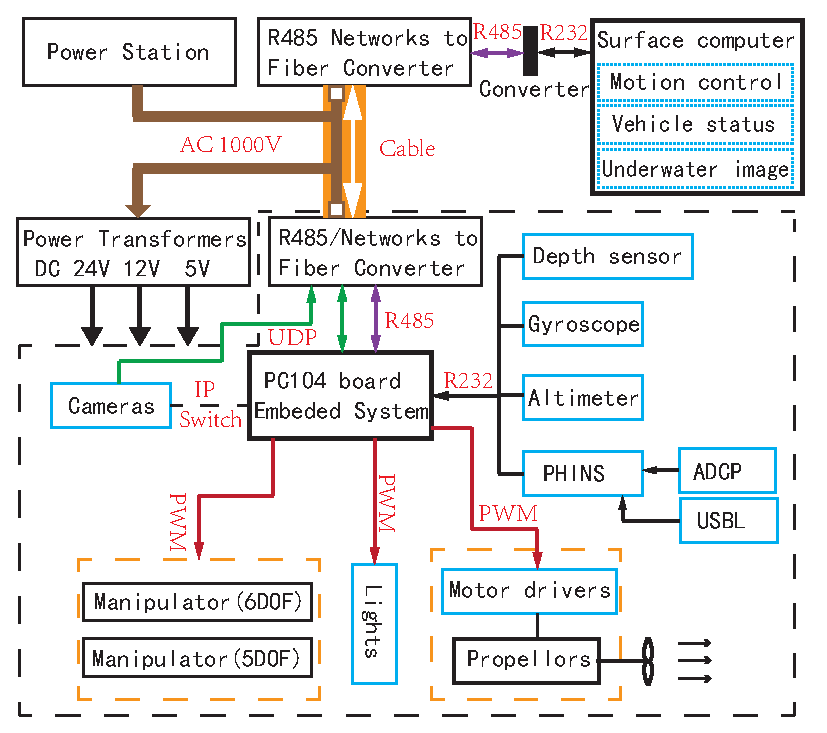
\includegraphics[width=14cm]{figure/chap2/F3.eps}
%\captionsetup{justification=centering}
\label{fig:chap2:F5}
\bicaption[fig:chap2:F5]{ROV 的系统控制框图}{ROV 的系统控制框图}{Fig.}{Diagram for ROV control system}
\end{figure}


\subsubsection{具有复杂形状的水下机器人数学模型 }

A. SJ-ROV 概况

SJ-ROV 3000 水下机器人是一款深海工作的ROV,其前置有两个机械手,可用作控制理论、水下科考等研究的实验平台。该型水下机器人由上海交通大学开发,具有多种工作模式,能够接受期望指令,并进行高精度导航寻迹控制\cite{lekkas2013line}。此外,当ROV的动力定位模式被打开时,该型水下机器人也可用来采集水下样本等。不同于海龙二号ROV\cite{xu2005deeprov,Huo2016Impulse},该型水下机器人推进器是电机驱动。机器人的关键部件,如压力舱体、动力系统、通信系统已经完成了测试,可以确保机器人工作的安全性与可靠性。目前,在一个最大深度为11m,长度为10m,宽度为6m的室内实验池内完成了初次航行实验\ref{fig:chap2:F3}。水下机器人的外形见图\ref{fig:chap2:F1},关键参数可以参考列表\ref{T2:chap2}。


B. 观测与通信系统介绍

SJ-ROV 3000由于设计目标为水下3000米,属于海况未知且复杂的环境,为了提高水下机器人的工作性能与定位能力,装载了诸多高性能的传感器,以期实现水下高性能航行的实验目标。在本部分,传感器的安装位置如图\ref{fig:chap2:F4}已经被标示出。表\ref{T3:chap2}列出了该型ROV水下机器人上安装的传感器的名称与类型。为便于进行系统理解,水下机器人的控制与通信框图也在本部分给出,见图\ref{fig:chap2:F4}。在惯性测量单元(INS)、多普勒测速仪(APDL)、深度计等这些传感器的帮助下,可以采集到ROV的姿态位置、速度以及深度的测量信息。并且,该型水下机器人配置有前、后视觉摄像头、水下灯、两个机械手以及用于和水面控制台通信的超短基线模块(USBL)。


该型ROV是由岸上供电,通过使用电源转换模块,经过动力缆给水下设备供电。通信和控制的测试是在实验水池完成的,水密性和动力也均被测试。控制测试是采用RS-485协议来发送命令,通过水下缆线中的光纤,将命令成功地发送到水下航行器上。图像观测和数据采集也通过光纤被采集并显示到水面控制台的显示器上。

C. 建模

根据ROV的推进器布置示意图\ref{fig:chap2:F4},可以确定该型ROV有7个推进器,当水下机器人处于完全在水里的状态时,在各个自由度上均有直接的推进器推力,也就是ROV系统可以拥有任何自由度的瞬间加速度,${rank}[\bm{f}_2(\bm{q},{\dot{\bm{q}}},t)]=dim[\bm{q}] =6$, 因此该系统的控制输入是不小于系统自由度数目的。

Fossen提出的6自由度的水下机器人动力学模型是非线性的,可用于对该型ROV的模型简化。ROV的自重较大,因此水下机器人推重比(最大推力/重量)较小,使得水下机器人的模型对于环境与模型中的动态变化并不敏感。配载的传感器变化以及流体阻力带来的影响对于水下机器人的控制而言并不明显。因此,在对ROV进行建模的时候,需对Fossen提出的模型做简化处理。

\begin{equation}
\label{eq:5}
\bm{M} \bm{\dot \nu} + \bm{D} \bm{\nu} =  \bm {\tau }
\end{equation}
式中,惯性质量矩阵$\bm{M}$ 可以使用机械设计软件求出。航行器受到的阻力,很难进行实际测定。简化会主要考虑流体阻尼。一般使用流体力学软件模拟求出阻尼力项$\bm{D}$。由于水下机器人是ROV工作模式,运行速度足够小,因此,受到的阻力主要是非线性项。其余力学影响,在建模时很难被求解出来,一般作为模型不确定性和干扰来应对。

工程控制实践中为了方便以及减少建模的困难,常常采用PID方法来设计控制器,会将恢复力(矩)、流体阻力、科氏力及产生阻力、附加质量以及环境和动力缆中的干扰力等均不进行建模,而是通过使用PID控制器计算期望状态与实际状态的误差,将PID控制器的输出值分配给不同的推进器上,从而实现控制的目的。具体的方法在本章\ref{2_3}节中给出。


\subsubsection{鱼雷型水下机器人数学模型  }

通过理论分析和经验数据获得的REMUS 100 AUV的6自由度非线性系统模型是为改进REMUS的控制提供了更精确的机器人平台模型。在本节中将对REMUS 100 AUV进行模型与配置详细介绍。REMUS的坐标系以及模型外观示意如图\ref{fig:chap2:F6},图中各个参数量的表示可以参考表\ref{tab:chap2:notation}。该型水下机器人仅仅拥有一个螺旋桨推进器固定在尾部,有四个舵片,一对水平舵,一对垂直舵,以十字形式固定在尾部推进器的周围。由于REMUS工作的控制是具有6个自由度的,而只有3个驱动器,因此REMUS AUV是系统控制输入是小于系统自由度的,控制难度高。

 \begin{figure}[!htp]
 \centering
 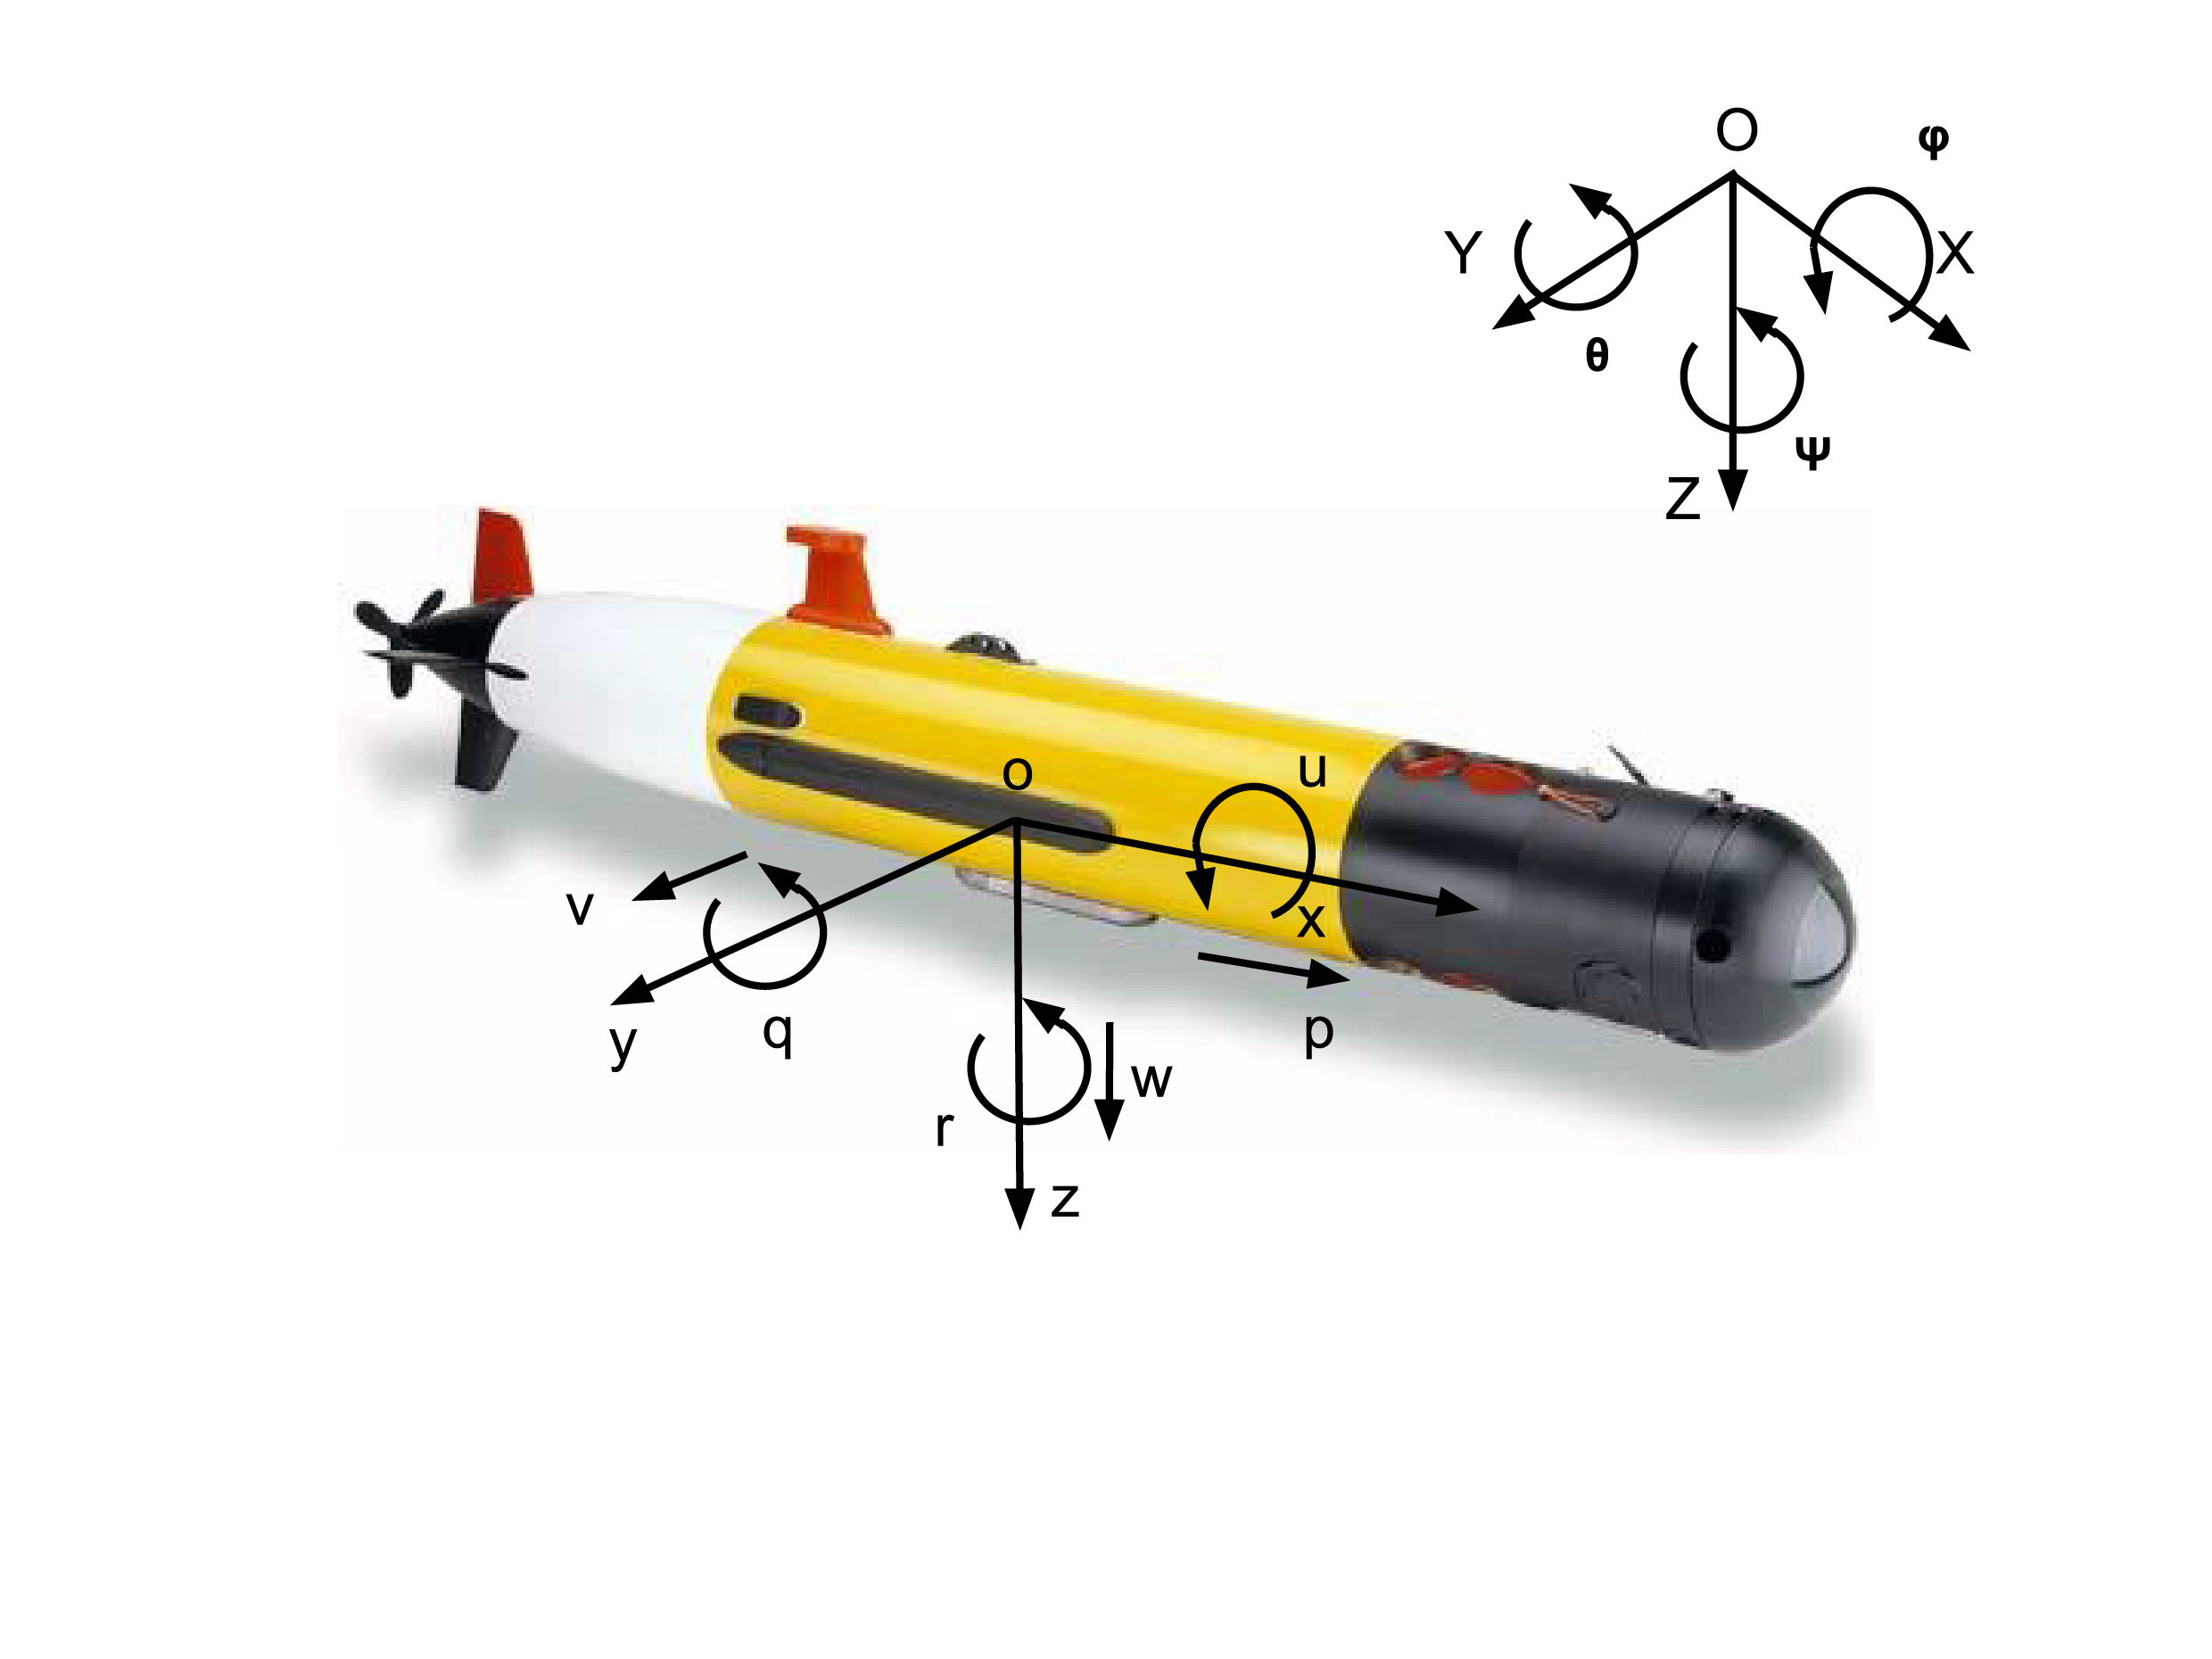
\includegraphics[width=11cm]{figure/chap2/REMUS_paper-300ppi.png}
 \label{fig:chap2:F6}
 \bicaption[fig:chap2:F6]{REMUS模型以及体坐标系、惯性坐标系示意}{REMUS模型以及体坐标系、惯性坐标系示意} {Fig}{REMUS body frame and inertial reference frame\cite{wu2016parametric}}
 \end{figure}

REMUS 100 AUV的载体坐标系原点位于几何中心上,因此浮心与几何中心重合。重心略低于浮心,处于靠下的位置。REMUS航行器的模型也可使用Fossen提出的非线性模型。左侧为刚体动力学,右侧为外部作用力和力矩。前面已经讨论了B-frame原点与浮心重合的情况,这样REMUS模型的左侧刚体动力学可以使用式\ref{eq:chap2:16}的形式。由于REMUS中的驱动器有舵片和推进器两种,舵片和航行器本体存在力学耦合,要建立其模型相对复杂。Prestero\cite{prestero2001verification} 使用实验中的测量数据建立REMUS的精确非线性模型,该模型中AUV的强非线性、多自由度耦合性以及系统静不稳定特点都反映了出来,具有很大贡献。

由水下机器人的重力和浮力而产生的流体静力、舵片驱动器产生的控制力,附加质量、流体动力学力以及推进器产生的推力和扭矩都被包含在REMUS的6自由度非线性模型里面。考虑到上述的力和力矩,结合式\ref{eq:chap2:30}给出REMUS的各个自由度方程如下:
纵荡(Surge):
\begin{equation}
\label{eq:chap2:surgeremus}
\begin{aligned}
m &\left[ \dot u - vr  + wq - {x_G}({q^2} + {r^2}) + {y_G}(pq - \dot r) + {z_G}(pr + \dot q) \right] =  \\
&- (W - B)\sin \theta  + {X_{u\left| u \right|}}u\left| u \right| + {X_{\dot u}}\dot u + {X_{wq}}wq\\
&+ {X_{qq}}qq + {X_{vr}}vr + {X_{rr}}rr + {X_T}  \\
\end{aligned}
\end{equation}
横荡(Sway):
\begin{equation}
\label{eq:chap2:swayremus}
\begin{aligned}
 m&\left[ {\dot v - wp + ur - {y_G}({r^2} + {p^2}) + {z_G}(qr - \dot p) + {x_G}(qp + \dot r)} \right] =\\
 & (W - B)\cos \theta \sin \varphi  + {Y_{v\left| v \right|}}v\left| v \right| + {Y_{r\left| r \right|}}r\left| r \right| + {Y_{\dot v}}\dot v + {Y_{\dot r}}\dot r \\
 &+ {Y_{ur}}ur + {Y_{wp}}wp + {Y_{pq}}pq +  {Y_{uv}}uv + {Y_{uu\delta }}{u^2}{\delta _r}  \\
\end{aligned}
\end{equation}
垂荡(Heave):
\begin{equation}
\label{eq:chap2:heaveremus}
\begin{aligned}
 m&\left[ {\dot w - uq + vp - {z_G}({q^2} + {p^2}) + {x_G}(rp - \dot q) + {y_G}(rq + \dot p)} \right] =\\
 & (W - B)\cos \theta \cos \varphi  + {Z_{w\left| w \right|}}w\left| w \right| + {Z_{q\left| q \right|}}q\left| q \right| + {Z_{\dot w}}\dot w \\
 &+ {Z_{\dot q}}\dot q + {Z_{uq}}uq + {Z_{vp}}vp + {Z_{rp}}rp + {Z_{uw}}uw + {Z_{uu\delta }}{u^2}{\delta _e}  \\
\end{aligned}
\end{equation}
横滚(Roll):
\begin{equation}
\label{eq:chap2:rollremus}
\begin{aligned}
 {I_x}\dot p + &({I_z} - {I_y})qr + m[{y_G}(\dot w - uq + vp) - {z_G}(\dot v - wp + ur)] = \\
 &({y_G}W - {y_B}B)\cos \theta \cos \varphi  - ({z_G}W - {z_B}B)\cos \theta \sin \varphi \\
 & + {K_{p\left| p \right|}}p\left| p \right| + {K_{\dot p}}\dot p + {K_{prop}}  \\
\end{aligned}
\end{equation}
俯仰(Pitch):
\begin{equation}
\label{eq:chap2:pitchremus}
\begin{aligned}
 {I_y}\dot q + &({I_x} - {I_z})rp + m[{z_G}(\dot u - vr + wq) - {x_G}(\dot w - uq + vp)] = \\
 &- ({z_G}W - {z_B}B)\sin \theta  - ({x_G}W - {x_B}B)\cos \theta \cos \varphi  \\
 &+ {M_{w\left| w \right|}}w\left| w \right| + {M_{q\left| q \right|}}q\left| q \right|
  + {M_{\dot w}}\dot w + {M_{\dot q}}\dot q  + {M_{uq}}uq \\
   &+ {M_{vp}}vp +{M_{rp}}rp + {M_{uw}}uw + {M_{uu\delta }}{u^2}{\delta _e} \\
\end{aligned}
\end{equation}
偏航(Yaw):
\begin{equation}
\label{eq:chap2:yawremus}
\begin{aligned}
 {I_z}\dot r + &({I_y} - {I_x})pq + m[{x_G}(\dot v - wp + ur) - {y_G}(\dot u - vr + qw)] = \\
 &({x_G}W - {x_B}B)\cos \theta \sin \varphi  - ({y_G}W - {y_B}B)\sin \theta  \\
 &  + {N_{v\left| v \right|}}v\left| v \right| + {N_{r\left| r \right|}}r\left| r \right|  + {N_{\dot v}}\dot v  + {N_{\dot r}}\dot r + {N_{ur}}ur \\
 &  + {N_{wp}}wp  + {N_{uv}}uv + {N_{pq}}pq + {N_{uu\delta }}{u^2}{\delta _r} \\
\end{aligned}
\end{equation}
式中,各个系数都是使用REMUS的水池实验数据推导出的。每个系数的具体解释可以参考Prestero的论文附录\cite{prestero2001verification}。其中, $X_{u\left| u \right|}, X_{\dot u}, X_{wq},X_{vr},X_{qq}, X_{rr}$ 是x方向的阻力、附加质量系数。同样,在上面的公式中可以给出别的自由度的流体阻力和附加质量系数。需要注意的是,$Y_{ur},Z_{uq},N_{ur},M_{uq}$ 表示的是附加质量和舵片力的合力作用。$ M_{uw},N_{uv},Y_{uv},Z_{uw}$ 是考虑舵片升降力、体升降力及转矩的力学系数。 $Y_{uu\delta },Z_{uu\delta },N_{uu\delta},M_{uu\delta },X_T,K_{prop}$ 是与控制舵片和推进器有关的流体动力学系数。

\section{推进器布置与推力控制向量 }
\label{2_3}
\subsection{推进器布置 }
\subsubsection{常见的布置 }

对于水下机器人常用的推进器是:
一. 可旋转方向推进器:该类型驱动器可以绕固定推进器的轴(z-axis)旋转以产生不同的推力,在推进器的体坐标x-y平面内都可以产生推力$(F_x,F_y)$。这种类型的推进器有很大的优势,因其可以减少整体设备的功率,也适用更多的可能情况。不过,这种类型的推进器由于机械结构复杂增加了控制的复杂性与难度。
二. 固定式推进器:固定方向的推进器因其推进器的中轴线相对于水下机器人本体夹角固定而定义。因这种类型的推进器是提前固定好的,不能随着任务的变化而调整。本章重点分析这种推进器。
三. 槽道推进器:这种推进器是放置在水下机器人的壳体通道内,可以进行正反旋转,产生推力。这种推进器多用在形状有要求的水下机器人中。
四. 控制面:控制面多使用舵片,可以固定在不同的位置以产生升降力和阻尼力,这种控制面和鳍类似,可以用于俯仰,偏航等运动中。

\begin{figure}[h]
    \centering
        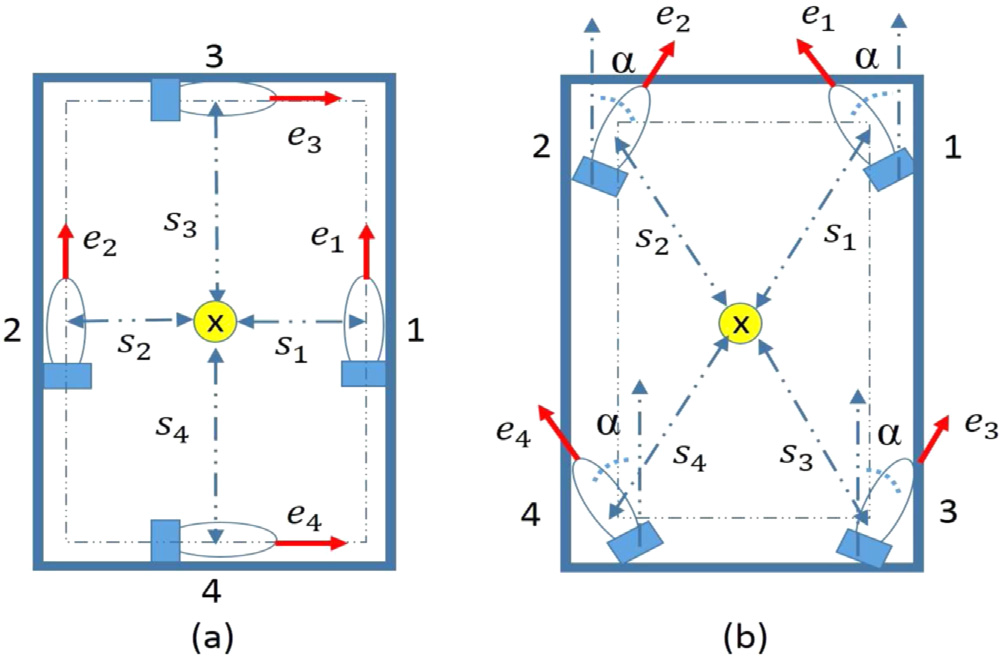
\includegraphics[width=12cm]{figure/chap2/configure.jpg}
        \label{fig:chap2:F7}
        \bicaption[fig:chap2:F7]{推进器的布置形式:左图:十字形式;右图:X 形式}{推进器的布置形式:左图:十字形式;右图:X 形式} {Fig}{Thruster configuration of vehicle: cross-shaped configuration(Left) and X-shaped configuration(right)}
\end{figure}

本工作将展示几种不同的推进器布置,这些是商业和科研水下机器人经常用的布置形式。在水下机器人的水平运动面内,有两种形式,十字形式和 X 形式, 如图\ref{fig:chap2:F7}\cite{dos2016bank}。十字形推进器布置又称为轴向布置,优点是该种布置形式下各个自由度的运动耦合性小。X形式布置又被称为矢量布置,它的优点是可以实现水平面内的各个自由度的运动控制。

水下机器人有很多种功用,也因此会衍生出很多个推进器布置形式,除了文中的布置形式还有如图\ref{fig:chap2:F8}所示的布置形式\cite{ardusub}。图中a和c图都是具有6个自由度的运动,均是全驱动系统,不同的是两种布置形式分别是从X形状和十字形状变化而来。b和d图中分别是5自由度和3自由度布置形式,b图中的布置经常用于水下机器人中,具有很好的推进器性能和灵活性;d图中的布置经常用于小型水下无人中,使用的推进器少,结构简单,可满足使用的基本功能要求。

\begin{figure}
%\begin{tabular}{cc}
\begin{minipage}{0.48\linewidth}
  \centerline{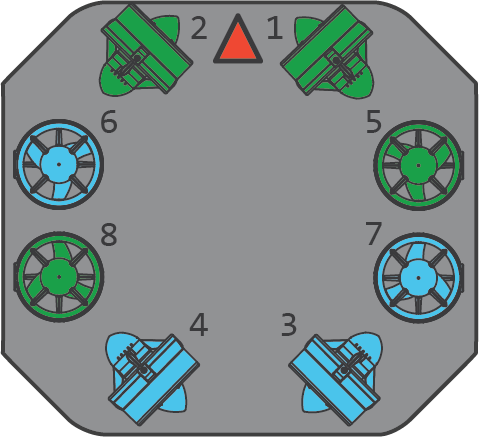
\includegraphics[width=4.0cm,height = 5cm]{figure/chap2/vectored6dof-frame.png}}
  \centerline{(a) 载重6自由度作业型布置}
\end{minipage}
\hfill
\begin{minipage}{.48\linewidth}
  \centerline{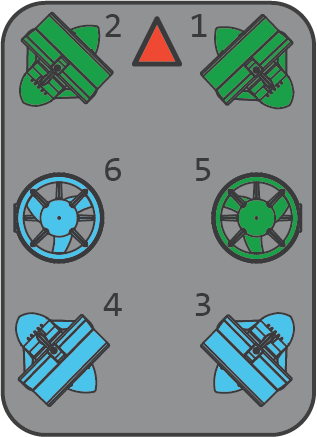
\includegraphics[width=4.0cm,height = 5cm]{figure/chap2/vectored-frame.png}}
  \centerline{(b) 5自由度布置}
\end{minipage}
\vfill
\begin{minipage}{0.48\linewidth}
  \centerline{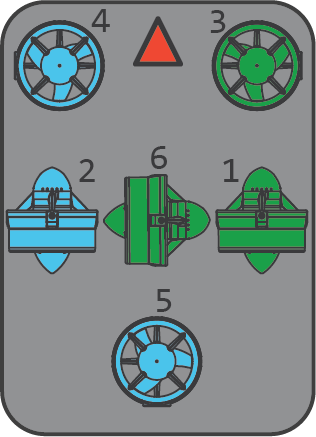
\includegraphics[width=4.0cm,height = 5cm]{figure/chap2/bluerov-frame.png}}
  \centerline{(c) 6自由度定位型布置}
\end{minipage}
\hfill
\begin{minipage}{0.48\linewidth}
  \centerline{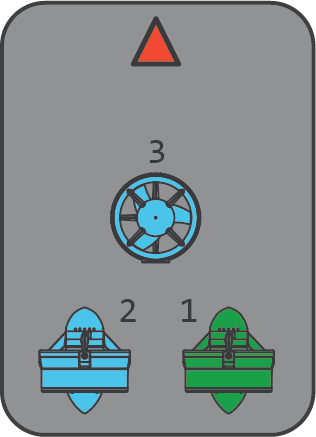
\includegraphics[width=4.0cm,height = 5cm]{figure/chap2/simplerov-3.png}}
  \centerline{(d) 3自由度布置}
\end{minipage}
%\end{tabular}
\label{fig:chap2:F8}
\bicaption[fig:chap2:F8]{水下机器人常用布置}{水下机器人常用布置} {Fig}{Congfiguration used in vehicle mostly\cite{ardusub}}
\end{figure}

\subsubsection{推力分配模型 }
电动螺旋桨推进器常常被用来驱动水下机器人。根据推进器布置的方式,这些推进器被划分为水平螺旋桨  $T_H$和垂直螺旋桨 $T_V$。正如图\ref{fig:chap2:F4}所示的一种形式,图中有四个水平置螺旋桨推进器 ,分别被图中标号为1, 2, 3, 4。图中5, 6, 7标识的为垂直放置推进器。水下推进器安装也有多种形式,对于SJ-3000 ROV, 水平推进器布置是X形式,这样可以提高推进器在水平面内的控制便捷性。中间的两个垂直推进器之间有夹角,也便于调节ROV的横滚运动。因此,本文给出推进器的布置形式与水下机器人的受力和力矩的数学关系如下\cite{dos2016bank}:

\begin{equation}
\label{eq:chap2:thrustconfigure_1}
  \begin{array}{l}
   {\bm \tau} = \bm{BT} \\
  \end{array}
\end{equation}
式中,$\bm{B}$表示螺旋桨推进器的布置矩阵,$\bm{T}$ 表示各推进器的推力组成的向量,向量的长度为推进器的个数$N$。对于文中的3000m的ROV,推力向量$\bm{T} = [T_1,T_2,T_3,T_4,T_5,T_6,T_7]^T$。$\bm{B}$ 是6*N的矩阵,且一般情况下,布置矩阵不是方阵。

为了更方便描述水下机器人的运动,常常会将6自由度的运动分为水平面运动和垂直面运动。因此,水下机器人受到推力$\bm \tau$也可以分为水平面合力 $\tau_H$ 和垂直面合力 $\tau_V$,这些力都是由推进器产生,但会对因为所处的运动不同,而在不同的运动面内对水下机器人的力学效果也有所差异。同样,\\
\begin{eqnarray}
\label{eq:chap2:BvBh}
\centering
T &=& \left[ {\begin{array}{*{20}{c}}
   {{T_H}}  \\
   {{T_V}}  \\
\end{array}} \right]\\
B &=& [\begin{array}{*{20}{c}}
    {{B_H}} & {0_{3\times3}}  \\
    {0_{3\times4}} & {{B_V}}  \\
\end{array}]
\end{eqnarray}
是根据推进器布置情况和运动面定义的推进器推力向量与分布矩阵。对于文中的ROV,$T_H = [T_1, T_2, T_3, T_4]^T$, $T_V = [T_5,T_6,T_7]^T$ 分别为水平面、垂直面的有贡献的推进器的推力。

确定了单个推进器推力以及推进器与运动的关系,可给出ROV的六个自由度方向上的推力分配方程。
\begin{equation}
\label{eq:chap2:thrustconfigure_2}
     \left[ \begin{array}{*{20}{c}}
     \tau_H\\
     \tau_V\\
     \end{array}\right]
      =
     [\begin{array}{*{20}{c}}
     {{B_H}} & {0_{3\times3}}  \\
     {0_{3\times4}} & {{B_V}}  \\
     \end{array}]\left[ {\begin{array}{*{20}{c}}
     {{T_H}}  \\
     {{T_V}}  \\
     \end{array}} \right] \\
\end{equation}
式中,$\tau_H = [\tau_{surge},\tau_{sway},\tau_{yaw}]^T$ 和 $\tau_V=[\tau_{heave},\tau_{pitch},\tau_{roll}]^T$。需要注意的是,水平面和垂直面的划分因水下机器人而异,本文的建立的推力分配矩阵是以3000m ROV为例,进行的分析。

本文中的推进器是由无刷直流电机带动螺旋桨而产生推力,该电机的最大转速是1850 $rpm$。推进器的推力线性特性较好,大大减轻了推进器性能差而控制困难的问题。推进器的模型是通过敞水实验获得的,参考模型是公式\ref{eq:chap2:29},但由于推进器正反推力最大值不同,获得推进器模型如下\cite{wunl2011immune}:

\begin{equation}
\label{eq:8}
{T_i} = \left\{ {\begin{array}{*{20}{c}}
   {{\gamma _1}{n^2}} & {if}  \\
   {{\gamma _{^2}}{n^2}} & {if}  \\
\end{array}} \right.\begin{array}{*{20}{c}}
   {{T_{i - }}_{\max } = 120kgf} & {forward}  \\
   {{T_{i - }}_{\max } = 90kgf } & {reverse}  \\
\end{array}
\end{equation}
式中 $\gamma _1 > 0$ 和 $\gamma _2 < 0$ 为推进器的正反推力系数。

应当指出的是螺旋桨推进器的叶片有逆时针和顺时针两种,这两种叶片也文中的ROV中成对使用,以便互相抵消扭矩。

\subsection{推力控制向量 }
\subsubsection{定义}
传统的推力分配时,等式\ref {eq:chap2:thrustconfigure_1}和\ref{eq:chap2:thrustconfigure_2}经常通过使用$\bm{B}$的伪逆矩阵来求解各推进器上的推力分布。然而,本文中的例子ROV,用于控制深度的螺旋桨推进器有三个,但并不总是每个推进器都是最佳选择,例如靠近ROV尾部的第七螺旋桨 $T_7$ 。实际上,使用 $T_5$ 和 $T_6$ 将更好地解决的深度控制问题。此外,有时需要根据ROV的功能来修改螺旋桨的布置形式,因此计算的布置矩阵会因某个推进器的变化而整体受影响,这对于系统的稳定并不是好的方案。单个推进器因布置位置的不同而可能对水下机器人的每个自由度的运动产生影响,那么是否可以考虑对单个推进器在整体运动中的作用来描述单个推力与整体运动所需控制力的关系呢?首先,要确定要描述推进器对每个自由度的影响的数学方程。本文提出使用推力控制向量来表征运动和推力的关系。一般在状态反馈控制中,ROV受到的实际力是不可以测量的,而是通过姿态传感器的实际值与期望值进行对比,将反馈误差输入控制器,控制器的输出便是$\bm{\tau_{Desired} }$,就是期望的合推力。而推力分配矩阵的最大目的就是将$\bm{\tau_{Desired} }$ 有效地分配给各个有关的推进器,但用于控制的推力控制向量与运动学的描述并不相同,该向量面向于控制而非数学中的力分配。推力控制向量如下\cite{ardupilot,ardusub}:
\begin{equation}
\label{eq:chap2:motor_factor}
\bm{\beta}_{i}=
\left[
\begin{array}{*{20}{c}}
  {f}_{surge}\\
  {f}_{sway}\\
  {f}_{heave}\\
  {f}_{roll}\\
  {f}_{pitch}\\
  {f}_{yaw}\\
\end{array}
\right]
\end{equation}
式中,$i$表示第 $i$ 个推进器。向量从上到下依次为电机纵荡系数(MOT SURGE FACTOR)、电机横荡系数(MOT SWAY FACTOR)、电机垂荡系数(MOT HEAVE FACTOR)、电机横滚系数(MOT ROLL FACTOR)、电机俯仰系数(MOT PITCH FACTOR)、电机偏航系数(MOT YAW FACTOR)。

因此,即使螺旋桨的布置发生变化,可通过将螺旋桨的推力控制矢量加入(Add)或删除(Delete)到ROV控制系统的推进器加载系统中进行推进系统快速升级,也可以合理地设定各个螺旋桨的推力控制向量中的各个自由度运动的有效力系数,而不必影响原有的控制方法以及其他推进器,如代码\ref{thrustercode:chap2}。在下一部分中,每个推进器的系数将根据控制模式设置并构成新的推力分布矩阵。\\

\begin{lstlisting}[language={C}, caption={ROV的推力布置示例\label{thrustercode:chap2}}][b]
static Thruster SJ_ROV_3000[] ={
       Thruster(0, MOT_1_SURGE_FACTOR, MOT_1_SWAY_FACTOR, MOT_1_HEAVE_FACTOR, MOT_1_ROLL_FACTOR, MOT_1_PITCH_FACTOR, MOT_1_YAW_FACTOR),
       Thruster(1, MOT_2_YAW_FACTOR, MOT_2_SURGE_FACTOR, MOT_2_SWAY_FACTOR, MOT_2_HEAVE_FACTOR, MOT_2_ROLL_FACTOR, MOT_2_PITCH_FACTOR),
       Thruster(2, MOT_3_SURGE_FACTOR, MOT_3_SWAY_FACTOR, MOT_3_HEAVE_FACTOR, MOT_3_ROLL_FACTOR, MOT_3_PITCH_FACTOR, MOT_3_YAW_FACTOR),
       Thruster(3, MOT_4_SURGE_FACTOR, MOT_4_SWAY_FACTOR, MOT_4_HEAVE_FACTOR, MOT_4_ROLL_FACTOR, MOT_4_PITCH_FACTOR, MOT_4_YAW_FACTOR),
       Thruster(4, MOT_5_SURGE_FACTOR, MOT_5_SWAY_FACTOR, MOT_5_HEAVE_FACTOR, MOT_5_ROLL_FACTOR, MOT_5_PITCH_FACTOR, MOT_5_YAW_FACTOR),
       Thruster(5, MOT_6_SURGE_FACTOR, MOT_6_SWAY_FACTOR, MOT_6_HEAVE_FACTOR, MOT_6_ROLL_FACTOR, MOT_6_PITCH_FACTOR, MOT_6_YAW_FACTOR),
       Thruster(6, MOT_7_SURGE_FACTOR, MOT_7_SWAY_FACTOR, MOT_7_HEAVE_FACTOR, MOT_7_ROLL_FACTOR, MOT_7_PITCH_FACTOR, MOT_7_YAW_FACTOR)
}
\end{lstlisting}

\subsubsection{PID控制应用实例 }
水下机器人的姿态控制是水下机器人控制中很重要的一项,一般是通过姿态角的依次控制来实现追踪期望命令。在刚刚接到控制命令时,首先要调整偏航角,这个阶段偏航角与俯仰角控制器不接收新的命令,以防止耦合影响。其次是调整俯仰角度,这时偏航角和横滚角度控制器不接收新的控制命令。最后是调节横滚角度。该种姿态控制方法经常被用于无人机上,可以通过使用PID控制器来完成高性能的任务\cite{mellinger2012trajectory}。水下机器人姿态控制器给出如下:

\begin{equation}
\label{eq:11}
\begin{array}{l}
 \Delta \varphi  = {k_{p,\varphi }}{e_\varphi } + {k_{i,\varphi }}\int {{e_\varphi }dt}  + {k_{d,\varphi }}{{\dot e}_\varphi } \\
 \Delta \theta  = {k_{p,\theta }}{e_\theta } + {k_{i,\theta }}\int {{e_\theta }dt}  + {k_{d,\theta }}{{\dot e}_\theta } \\
 \Delta \psi  = {k_{p,\psi }}{e_\psi } + {k_{i,\psi }}\int {{e_\psi }dt}  + {k_{d,\psi }}{{\dot e}_\psi } \\
 \end{array}
\end{equation}
式中,$k_p,k_i, k_d$为PID控制的控制参数。$\Delta \varphi, \Delta \theta, \Delta \psi$ 为PID输出的矫正力。

通过分析每个螺旋桨推进器的现有安装形式下水下机器人运动受到的力学影响,确定出推进器对每个姿态角的方向上的推力控制向量的系数。将获得的各推力控制向量进行组合,并将PID控制器的反馈矫正力分配到合适的推进器上,给出的计算公式如下:

\begin{equation}
\label{eq:12}
\left[ {\begin{array}{*{20}{c}}
   {{T_1}_{CMD}}  \\
   {{T_2}_{CMD}}  \\
   {{T_3}_{CMD}}  \\
   {{T_4}_{CMD}}  \\
   {{T_5}_{CMD}}  \\
   {{T_6}_{CMD}}  \\
   {{T_7}_{CMD}}  \\
\end{array}} \right] = \left[ {\begin{array}{*{20}{c}}
   0 & 0 & 1  \\
   0 & 0 & { - 1}  \\
   0 & 0 & { - 1}  \\
   0 & 0 & 1  \\
   1 & 0 & 0  \\
   { - 1} & 0 & 0  \\
   0 & 1 & 0  \\
\end{array}} \right]\left[ {\begin{array}{*{20}{c}}
   {\Delta \varphi }  \\
   {\Delta \theta }  \\
   {\Delta \psi }  \\
\end{array}} \right]
\end{equation}
其中公式\ref{eq:12}右边为推力控制向量矩阵与PID反馈的矫正力。推力控制向量矩阵的第\textit{i}行分别为第\textit{i}个推进器对姿态的各个自由度的力学系数。因为PID控制器的系数也是可以调节的,因此在推力控制向量中的系数可以定义为1, 0 , -1。

本节建立了推进器和控制器之间的推力分配关系,该分配关系可以选出对所需控制的运动最有效的推进器,如此ROV可以跟踪所要求的方向指令,并完成状态调整。

\section{本章小结 }

本章系统地引入了一般形式的水下机器人的坐标系、运动学状态转换方程、流体动力学模型,便于水下机器人进行后续的模型参数计算和控制应用;分析文中研究的两种不同外形的水下机器人,首先给出具有非初等几何外形的水下机器人的数学描述,而后给出该型水下机器人的简化模型;给出了鱼雷形状的水下机器人的数学模型,并分析了系统需要关注的系统动态特性。最后,根据推进器的空间布置,给出了不同形式的推力分配模型。分析建立的基于运动学的推力分配模型,提出面向控制的推力控制向量,着重利用对运动影响性强的推进器,并使用中水下机器人的PID姿态控制来进行实例化分析。

%# -*- coding:utf-8 -*-
%!TEX root = ../thesis.tex

\chapter{水下机器人数学模型搜索与环境识别 }

\label{chap:system_discovery}
% 3.1 引言
% 3.2 系统模型的结构与辨识
% 3.3 基于Levenberg-Marquardt 方法的参数辨识
% 3.4 基于遗传算法的参数辨识
% 3.5 基于符号回归技术的水下机器人模型搜索
% 3.6 基于支持向量机的水下机器人水流环境辨识
% 3.7 小结
\section{引言}

在许多领域的研究中,非线性系统的模型识别是至关重要的\cite{kim2012estimating}。开发的数学模型可以用于研究系统的潜在行为或者对系统进行监督、观测、以及预测系统的发展趋势。此外,数学模型还可以用于控制器,如模型预测控制中。各种系统识别技术被用于动力系统的建模中。

模型的概念已在越来越多的科学领域用来表示观测的系统,而模型的确定就是确定系统在时间中的演化过程\cite{wu2016parametric}。这个过程中,系统受到的力、状态和环境间的相互作用都会被描述。虽然目前的技术进步使得研究者越来越方便地去收集水下机器人的系统测量数据,但是在系统的模型参数化过程仍然受到数据集大小以及数据间的映射关系如模型的数学表达形式的太复杂特点的困扰\cite{menezes2014symbolic,wu2016parametric}。其中有环境的影响,如水流,另外也有噪声等因素的影响作用。
如果使用传统的科学方法,研究人员首先要学习或者建立可以解释水下机器人的数学模型,然后使用测量的数据或者计算方法来分别求解模型中关键项\cite{yang2014modeling,huang2015trends}。然而,
有时研究人员的视角是受到人们固有的知识结构限制,也许模型的表述并不是最好的,而使用者却并不知道。问题在与人们偏爱与寻找能够清楚理解的好模型,而往往直觉确实是不正确的。另外的就是数据测量的运行环境并不能代表系统的所有运行情况,水下机器人的室内水池实验就大多是在静水中的测试,并没有考虑水流等因素。水下机器人系统从环境中获得的信息还很少,并不会主动地辨识环境,这就弱化了水下机器人在水下的生存能力。

水下机器人工作的环境未知多变,使得准确地描述机器人的数学模型并不太容易,其中尤其是非线性水下机器人系统。鱼雷型水下机器人往往比较难以控制,而且多是自主航行,因此要认识它的系统采用以往的方法并不一定可行。水下机器人的非线性的系统模型在上一章中被整理成矩阵形式,但仍需要确定实际系统中应用时的具体结构与参数\cite{garcia2014modelling,Tang2009Estimation,yang2014modeling}。本节将分析REMUS AUV的数学模型,并使用输出状态量与控制输入量,将模型向状态模型的形式变换,从数据驱动的系统建模角度分析水下机器人的模型\cite{brunton2016discovering,schmidt2009distilling}。上一章建立REMUS AUV系统模型,从模型的组成两部分来分析,模型的具体数学表达形式,即模型结构,已经确定。基于此确定的模型结构,仍然需要确定模型中各个参数量,这个过程就是系统辨识\cite{eng2014added}。系统辨识是基于输入和输出的数据以及确定模型形式的系统来确定参数的具体数值。

非线性系统模型的参数辨识已经获得了很大的进展,如本工作中使用的Levenberg-Marquardt算法和遗传算法\cite{baruch2009levenberg,zhou2013genetic}。不过,当所要辨识的目标系统的模型结构未知的时候,这类方法无法正确处理这类AUV系统的模型参数辨识问题。符号回归方法已经成功用于不被了解如何工作的系统的建模,仅仅使用输入输出数据,就可成功地确定出模型的数学表达,并具有难以置信的参数辨识准确率与速度\cite{menezes2014symbolic,Moreno2015Symbolic,wu2016parametric}。不同的是,用符号回归搜索的数学模型,使用基因表达树来表达模型,其本身可以由使用者指定或者自行演化确定。符号回归方法更适合用于搜索模型的数学近似结构,从另一个角度看待系统。

水下机器人工作的深海环境未知性较强,以往的研究给出了航行器受到的主要影响就是水流。深海有多种鱼类生存活动,但是水下机器人的水下工作经常面临不可以预计的危险,主要原因就是其对周围环境的认识能力受限。水下机器人对水下环境的认识能力相比于鱼类感知水环境的能力还相差很远\cite{verschure2003environmentally}。从生物学角度,鱼体侧线器官对水流环境和目标的识别改善了其生存能力。回顾了鱼类对水的感知的一些重要物理结构,特别是侧线系统的感知细胞。在侧线系统的帮助下,鱼可以感知周围的环境,通过感知神经网络受到的刺激信号,将产生神经信号并传输猎物的位置到鱼的大脑\cite{abdulsadda2012artificial,Wu2016lateralline}。神经信号的刺激由侧线系统的生物传感器产生,其中神经丘的机械变形在神经脉冲的表达中转化为压力信号。神经脉冲的处理过程,就是鱼从大量数据中学习水流的模式,可为水下机器人认识水下环境提供参考方法\cite{huang2015trends,martis2013ecg,chen2000new,liu2012support,tagliaferri2015wind}。本章使用获取的水下机器人体周的压力数据,基于数据的稀疏特性将其降维,并使用机器学习方法进行水流方向和速率大小的识别训练与测试,从而让水下机器人更好地认识和利用海洋。

\section{水下机器人模型搜索与参数辨识 }

水下机器人的模型主要包括模型的结构和参数两个主要的部分,本节主要研究非线性6自由度系统模型的水下机器人模型搜索与辨识问题。首先介绍从水下机器人系统中获得的测量数据是如何和系统的模型结构和参数联系起来,分析模型结构已知的辨识方法与未知的方法上的区别。其次是使用Levenberg-Marquardt方法、遗传算法和符号回归方法来对REMUS AUV的模型的参数辨识进行研究,辨识共47个流体动力学参数。最后将对比各个方法辨识水下机器人模型参数的结果,并尝试用符号回归方法搜索用于近似结构的模型,这种近似模型可以用于控制研究。

\subsection{系统模型的结构、参数与系统建模}

在本部分,为了便于后面的系统建模,需要对一个动力学系统的建模问题从黑盒子的角度进行最初的研究。一般要研究的系统会有状态量和输出、输入量。要确定一个系统模型表达,需要收集时间序列的状态数据$\bm{X}$(包括状态量及导数量)。将得到的采样数据写成如下两个矩阵\cite{brunton2016discovering}:
\begin{equation}
\label{eq:chap3:1}
\begin{aligned}
\bm{X} &= \begin{matrix}
\\
\begin{bmatrix}
 \small \bm{X}^T(t_1)     \\
 \small \bm{X}^T(t_2)     \\
 \small \vdots            \\
 \small \bm{X}^T(t_{m})   \\
\end{bmatrix}
 \end{matrix}
= \begin{matrix}
  \rightarrow {state}  \\
  \begin{bmatrix}
   x_1(t_1) & x_2(t_1) & \ldots & x_n(t_1) \\
   x_1(t_2) & x_2(t_2) & \ldots & x_n(t_2) \\
   \vdots   & \vdots   & \ddots & \vdots   \\
   x_1(t_m) & x_2(t_m) & \ldots & x_n(t_m) \\
  \end{bmatrix}
  \downarrow time \\
 \end{matrix}
% \end{equation}
\\
% \begin{equation}
% \label{eq:chap3:2}
\dot {\bm{X}} &=
\begin{bmatrix}
 \small \dot {\bm{X}}^T (t_1)     \\
 \small \dot {\bm{X}}^T(t_2)      \\
 \small \vdots                 \\
 \small \dot {\bm{X}}^T(t_{m}) \\
\end{bmatrix}
= \begin{bmatrix}
   \dot{x_1}(t_1)  &  \dot{x_2}(t_1) & \ldots & \dot{x_n}(t_1) \\
   \dot{x_1}(t_2)  &  \dot{x_2}(t_2) & \ldots & \dot{x_n}(t_2) \\
   \vdots          &  \vdots         & \ddots & \vdots         \\
   \dot{x_1}(t_m)  &  \dot{x_2}(t_m) & \ldots & \dot{x_n}(t_m) \\
  \end{bmatrix}
\end{aligned}
\end{equation}

一个系统的表达主要是有多个不同符号功能组合而成的非线性函数,因此需要选定一个符号功能库,该库包括常数、多项式、三角函数:


\begin{equation}
\label{eq:chap3:3}
\bm{\Theta(\bm{X})}= \begin{bmatrix}
|      & |      &  |         &|           &        &|            &|          &         \\
\bm{1} & \bm{X} & \bm{X}^P_2 & \bm{X}^P_3 & \ldots & sin(\bm{X}) &cos(\bm{X}) & \ldots \\
|      & |      &  |         &|           &        &|            &|          &         \\
\end{bmatrix}
\end{equation}
其中,高阶多项式是就 $\bm{X}^P_2, \bm{X}^P_3$ 等,他们表达的就是模型中非线性功能项。 二次非线性项 $\bm{X}^P_2$ 比表达如下:

\begin{equation}
\label{eq:chap3:4}
\bm{X}^P_2 = \begin{bmatrix}
x_1^2(t_1) &  x_1(t_1)x_2(t_1)   & \ldots & x_2^2(t_1) & \ldots &  x_n^2(t_1) \\
x_1^2(t_2) &  x_1(t_2)x_2(t_2)   & \ldots & x_2^2(t_2) & \ldots &  x_n^2(t_2) \\
\vdots     & \vdots              & \ddots & \vdots     & \ddots & \vdots      \\
x_1^2(t_m) &  x_1(t_m)x_2(t_m)   & \ldots & x_2^2(t_m) & \ldots &  x_n^2(t_m) \\
\end{bmatrix}
\end{equation}

对于水下机器人而言,式\ref{eq:chap3:1}中列就是某个自由度的状态输出量, 要确定水下机器人模型就是求解 $\bm{\Xi}$。
\begin{equation}
\label{eq:chap3:5}
\dot{\bm{X}} =
\bm{\Theta}(\bm{X}) \bm{\Xi}
\end{equation}
其中 $\bm{\Xi} = [\bm{\xi}_1, \bm{\xi}_2,\ldots,\bm{\xi}_n]$ 是系数矩阵。

一般在系统辨识中采用辨识方法多是基于最小二乘法的\cite{friedman2001elements},需要写出系统模型的目标函数,就需要对式\ref{eq:chap3:5}进行变换,从而更加利于辨识的执行。给出的目标函数的形式如下\cite{brunton2016discovering,wu2016parametric}:
\begin{equation}
\label{eq:chap3:6}
\dot{\bm{X}}_k = \bm{f}_k(\bm{X}) = \bm{\Theta}(\bm{X}^T)\bm{\xi}_k
\end{equation}
\begin{equation}
\label{eq:chap3:7}
\dot{\bm{X}}= {\bm{\Xi} }^T (\bm{\Theta}(\bm{X}^T))^T
\end{equation}

水下机器人的动力学系统也可表达成状态方程的形式,因此水下机器人的系统参数也可以使用基于最小二乘法的辨识方法\cite{baruch2009levenberg}。不过这种辨识方法是有个前提,即式\ref{eq:chap3:6}中的用于描述符号功能的块是必须已经确定。本章提出的符号回归方法可以同时对模型的结构部分与参数部分进行进化,并使用性能评判函数筛选最佳估计值。下面分别介绍Levenberg-Marquardt算法、遗传算法和符号回归算法用于参数辨识的例子。此外也使用符号回归算法搜索了模型结构未知时候的可能最佳近似模型。

\subsection{基于Levenberg-Marquardt方法的参数辨识 }

 Levenberg-Marquardt(LM)方法是对求取目标函数最小值的高斯牛顿方法一种受欢迎的替代选择,该方法具有高斯牛顿方法和梯度下降方法的两者优点,是一种有效的广义非线性最小二乘法算法\cite{baruch2009levenberg}。REMUS AUV 的动力学模型是非线性的,表达形式可以写成$y=f(x,\theta)$ 的形式,其中$x$ 是函数变量, $\theta$ 是需要识别的参数,水下机器人的最小二乘法问题可以定义为如下形式:

\begin{equation}
\label{eq:chap3:7}
F\left( \theta  \right) = \frac{1}{2}\sum\limits_{i = 1}^m {{{\left[ {{y_i} - f\left( {{x_i},\theta } \right)} \right]}^2}}
\end{equation}
式中,$y_i$ 是模型的估计值,$f(x_i,\theta)$ 是实际系统的值。辨识的过程就是求解式\ref{eq:chap3:7}的最小值的过程。

当平方和函数,$ F(\theta)$,为最小值时,平方和函数相对 $\theta$ 的梯度是为0的。由 $f(x_i,\theta+\delta)$ 的一阶近似可以给出如下平方和函数:

\begin{equation}
\label{eq:chap3:8}
{\rm{F}}(\theta  + \delta ) \approx \sum\limits_{i = 1}^m {{{\left( {{y_i} - f\left( {{x_i},\theta } \right) - {J_i}\delta } \right)}^2}}
\end{equation}

求出平方和函数相对于 $\delta$ 的导数形式,并令导数为0,则可以得到

\begin{equation}
\label{eq:chap3:9}
\left( {{J^T}J} \right)\delta  = {J^T}\left[ {y - f\left( \theta  \right)} \right]
\end{equation}
其中,$J$ 是第 $i$ 行等于 $J_i$ 的雅可比矩阵,其中$f$ 和 $y$ 分别是具有第 $i$ 个分量 $f(x_i,\theta)$ 和 $y_i$的向量。

Levenberg-Marquardt方法使用搜索方法来求出线性方程组的解,它通过使用“阻尼项”代替方程\ref{eq:chap3:9}的对应项,可以得到新得
\begin{equation}
\label{eq:chap3:10}
\left( {{J^T}J + \lambda I} \right)\delta  = {J^T}\left[ {y - f\left( \theta  \right)} \right]
\end{equation}
其中,\textit{I}是单位矩阵,并给出被估计参数向量的增量 $
\delta$,非负标量 $\lambda$ 是用来控制增量的步长和方向。


\subsection{基于遗传算法的参数辨识  }

遗传算法(GA)是一种模拟生物进化过程中的自然选择机制而求解问题的全局优化方法。对于水下机器人的非线性水动力学参数的辨识问题,一群个体组成的解的集合是基于适应度函数的评估不断进化以便选出最好的参数估计解\cite{yuan2010genetic,zhou2013genetic,chang2007nonlinear}。

适应度函数对于保持解的精度非常重要,本文将输出误差的加权值作为适应度函数来进行评估。如此,可以将参数辨识问题转变成为遗传算法的参数优化问题。

水下机器人的适应度函数定义如下:
\begin{equation}
\label{eq:chap3:11}
{J_j} = \sum\limits_{i = 1}^m {\left| {\frac{{{X_j}(i) - {{\hat X}_j}(i)}}{{{X_j}\left( i \right)}}} \right|}
\end{equation}
其中,$X=[u,v,w,p,q,r]$ 是水下机器人在体坐标系的状态向量,$X_j$ 是 $X$ 的第 $j$ 个量。

遗传算法的基本优化流程如下:\\
步骤1:随机生成群体,设置最大代数,以及其他终止条件。\\
步骤2:个体评估:计算种群 $P(t)$ 中每个个体的适应度函数。\\
步骤3:选择操作:根据适应度值对当前种群 $P(t)$ 应用选择操作。\\
步骤4:交叉操作:将交叉操作应用于种群 $P(t)$ 以产生下一代。\\
步骤5:突变操作:将变异操作应用于种群 $P(t)$ 。\\
在步骤3,步骤4,步骤5之后,根据所有的个体的适应度函数值可以得到下一代种群 $P(t)$ 。\\
步骤6:终止条件判断:如果 $t = T$ 满足其他终止条件,则处理中具有最合适适应度函数值的个体将被选为辨识问题的最优解。 否则,回到步骤2。\\

\subsection{基于符号回归技术的水下机器人模型搜索  }

\subsubsection{符号回归 }

回归分析是研究科学问题的基本方法之一。回归的任务是辨识输入变量 $x = [x_1, x_2,\ldots,x_j]$ 和 数据中不断变化的因变量 $y = [y_1, y_2, \ldots,y_k]$之间的数学关系。其中, $j$ 是每个观察值中的自变量的标号,$k$ 是因变量的标号。建立的数学关系为了确定自变量和因变量之间的映射关系,并测试搜索到的模型的质量和一般性。在回归过程中,辨识是从确定一个不确定的数学映射关系函数到识别一个预定义的目标函数的参数值。然而这意味着,参数可以由辨识方法自动的调节,而目标函数的结构必须由一个人类专家定义才可以。符号回归是一种基于遗传技术的用来搜索表达空间以减少多种评价函数误差量的回归方法\cite{schmidt2009distilling}。

符号回归可以估计水下机器人系统模型的参数并可同时改善方程式的结构表达。然而,传统的线性和非线性回归方法只能通过辨识具有预定方程结构的观测系统模型的参数值。虽然其他很多方法都可以辨识模型的参数值,但是符号回归方法因为可以对模型的数学表达式的结构上做操作,而优势明显。符号回归方法的主要思想是集中于搜索目标空间的可能解上,而放弃一些不大有希望的数学解空间。符号回归算法是通过模仿遗传和进化算法的机理来完成搜索任务的。符号回归中运算操作主要有突变、交叉、选择,这些都可以用来处理模型的代数数学表达式的进化。虽然机理来源相同,但是在具体的处理技术上有些差异,表达解的方法是多种多样\cite{dos2009nonlinear,Gandomi2012A1}。遗传编程是一个由生物自然演化启发的进化算法, 其中使用非正式和正式符号来改善模型的结构表达,以及提高大量数据处理应用中的计算效率,如符号回归。

在REMUS AUV模型的回归处理中,一个水下机器人模型的初始表达式由数据随机地从一群符号表达方程中选择出来。每一次进化中,通过重新组合以前的模型表达式,并使用交叉和突变处理以产生新的表达形式,这些解的个体会构成一个新的种群。每次进化得到的种群都和上一代的种群不相同。在每次选择处理中,对REMUS的数据建模比较好的模型会被存储下来。基因和编码被用来表达REMUS的数学模型的符号形式,以便于进行回归处理。如此,该方法将可以发现模型数据中最可能的数学表达方程,并可以用来解释隐藏在水下机器人观测数据中内在关系。

\subsubsection{遗传编程 }

遗传编程(GP)是一种符号优化技术,它使用基于达尔文自然选择原理创建计算机程序来解决给定的任务\cite{schmidt2009distilling,dos2014genetic,feng2006identification,garg2014mathematical}。 遗传编程和遗传算法之间的差异在于对问题解的表达方法不同。遗传算法中,以字符形式的数字被创建出来以表达解,而遗传编程中,通常使用树结构的形式来表达各个解,并将这些解构成一个计算程序的一部分。与遗传算法一样,遗传编程技术也是在全局范围内进行搜索的,并极力避免陷入到局部最优解的搜索困境,但是由于对于问题表达的规范性更强,操作处理更加准确。

正如符号回归部分所述,水下机器人系统建模的方程式的个体构成的群体随机地被创建出来以获得搜索解的多样性。群体中的每个成员都是一个包括功能集和数据变量集的分层结构树。表达个体的数据集和功能集是从程序预先设定的功能和变量集中选择出来的。例如,运算功能集中的函数表达F会包括基本代数运算操作符号(+, - ,*,/等等)、布尔逻辑函数(AND,OR,NOT等)或任何其他数学函数。变量数据集T则包含函数中各种参数,可以有数字常量、逻辑常数、变量等构成。函数中运算功能集和变量集中的各个元素被算法挑选出来组合在一起以获得水下机器人模型示例的基因型结构染色体表达,其中REMUS的某个自由度运动的数学方程包括功能和变量均会被存储为二进制的形式。图\ref{fig:chap3:F1}中示出了用于航行器偏航运动的简化方程\ref{eq:chap3:12}的GP模型的基因树表示的模型示例。

\begin{equation}
\label{eq:chap3:12}
 I\dot r = {N_{\dot v}}\dot v + {N_{\dot r}}\dot r + {N_v}v + {N_r}r + {N_{uu\delta }}{u^2}\delta
\end{equation}

\begin{figure}[!htp]
  \centering
  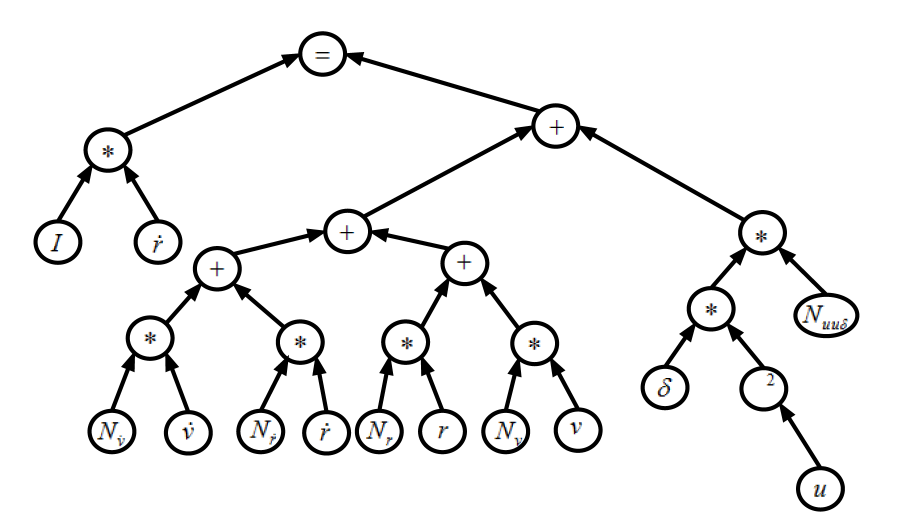
\includegraphics[width=14cm]{figure/chap3/gptrees.png}
  \label{fig:chap3:F1}
  \bicaption[fig:chap3:F1]{GP树表示的REMUS偏航方程}{GP树表示的REMUS偏航方程} {Fig.}{GP trees for the Yaw motion of REMUS(see equation(\ref{eq:chap3:12})) }
\end{figure}


遗传编程的初始种群的创建是在可能的解决方案的大空间中盲目搜索的一个可能的解决方案。一旦模型群体被随机创建出来,遗传编程方法将会开始评估种群的每个个体,并选择部份个体进行繁殖操作,并使用突变、交叉以及直接繁殖操作以产生新的个体。最后,在每次迭代中不断地创造出新的个体,并优化产生新群体\cite{Gandomi2012A2,stoutemyer2013can}。

交叉操作时,随机地选择每个解个体(程序)基因树的分支上的一个点,然后交换每个程序的变量集或功能集,这样可以创建出两个新程序个体(见图\ref{fig:chap3:F2})。在进化过程的每次迭代中,使用适应度函数值评估新群体,并开始新一轮的繁殖和交叉操作。在遗传编程算法的这个过程中,从模型中选择一个变量或功能符号,并使用变异操作(见图\ref{fig:chap3:F2})。在任何一代出现的最好的程序个体,以及至今最好的解个体,定义了遗传编程算法的输出\cite{Gandomi2012A1,schmidt2010symbolic}。

\begin{figure}[!htp]
\centering
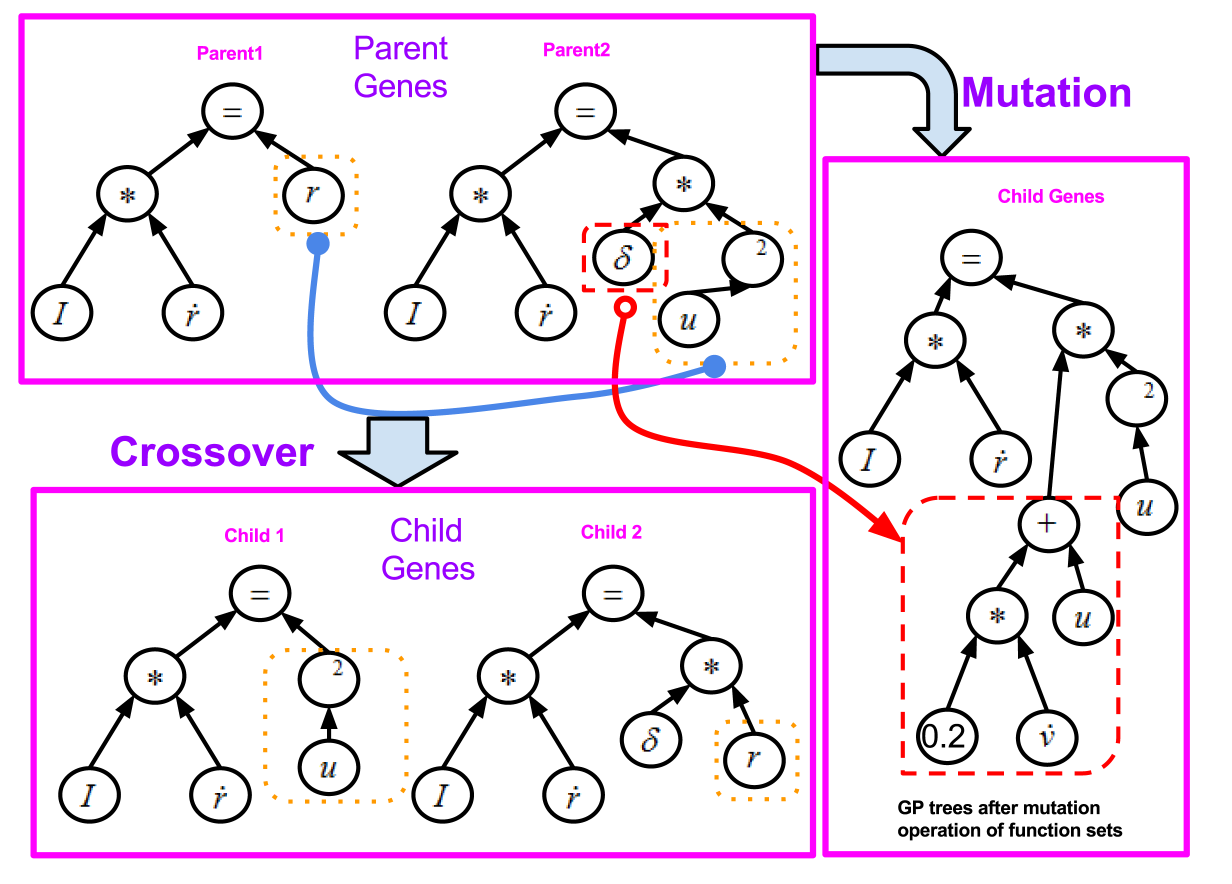
\includegraphics[width=14cm]{figure/chap3/GPevolution.png}
\label{fig:chap3:F2}
\bicaption[fig:chap3:F2]{遗传编程进化过程示意}{遗传编程进化过程示意} {Fig.}{Schematic of automatic evolution of Yaw motion equation using GP }
\end{figure}

根据计算返回的误差度量值,在进化的每个回归过程中,REMUS AUV的偏航运动模型的数学表达式将被预测和评估性能。虽然机器人的模型中包含非线性项(例如,$sin$,$cos$),但是遗传编程算法的运算可以用二进制编译方法将新形式的方程个体创建出来。在每一代的回归过程中,可以给出目标方程的具体表达,并可以从中确定流体力学系数的参数数值。根据提出的误差标准,符号回归获得的运动模型的质量好坏可以被检查和评估。因此,可以从训练数据中轻松地获得REMUS AUV的模型结构和系数。符号回归的求解过程比Levenberg-Marquardt算法和遗传算法等最小二乘法更为方便,计算甚至更准确。搜索REMUS模型的结构和参数表明,基于遗传编程技术的符号回归方法可以成功应用于水下机器人非线性模型的识别。

\subsection{结果与分析 }

本节将介绍Levenberg-Marquardt算法,遗传算法和符号回归方法的辨识水动力参数的估计结果,并使用符号回归方法搜索测量数据集以发现AUV模型的新形式。

A. 误差评估

使用符号回归、Levenberg-Marquardt方法、遗传算法对实验数据辨识的结果可以使用误差直接评估。 为了检查使用的辨识方法的性能,将计算平均绝对误差(MAE),均方误差(MSE)和混合相关/误差(HCE)。  MAE,MSE和HCE计算公式如下:

平均绝对误差(Mean Absolute Error):
\begin{equation}
MAE = \frac{1}{N}\sum\limits_{i = 1}^N {\left| {y - f\left( x \right)} \right|}
\label{eq:chap3:mae}
\end{equation}
假设噪声服从双指数分布,可以使用MAE缩小残差的绝对值。

均方误差(Mean Squared Error):
\begin{equation}
MSE = \frac{1}{N}\sum\limits_{i = 1}^N {{{\left( {y - f\left( x \right)} \right)}^2}}
\label{eq:chap3:mse}
\end{equation}
假设误差噪声服从正态分布,使用其可以缩笑均方残差值。

混合相关误差(Hybrid Correlation/Error):
\begin{equation}
HCE = \sum\limits_{}^{} {\sum\limits_{}^{} {\left( {\sum\nolimits_{X,Y} {} } \right)} }  + \frac{1}{N}\sum\limits_{i = 1}^N {\left| {y - f\left( x \right)} \right|}
\label{eq:chap3:hce}
\end{equation}
式中,将相关性和绝对误差进行组合。

在上面公式中,$y$ 是输出值, $f(x)$ 是目标值, $N$ 是测量的总数。MAE, MSE对于三个算法都适用,而HCE仅仅用于符号回归到评估中。

B. 初始设置与预处理

考虑到过程噪声对航行器模型系统的影响,REMUS模型的数值实验和参数识别是基于方程\ref{eq:chap2:30}和各个自由度的非线性方程\ref{eq:chap2:surgeremus}、\ref{eq:chap2:swayremus}、\ref{eq:chap2:heaveremus}、\ref{eq:chap2:rollremus}、\ref{eq:chap2:pitchremus}与\ref{eq:chap2:yawremus}进行的。测量的运动数据包括大量的噪声,水下航行器系统的非线性模型中的噪声通常被认为是高斯白噪声,假定为零均值高斯白噪声且是相互独立的\cite{sabet2014extended}。本文中用于航行器的建模参数估计的运动数据中包含的噪声被进行了预处理以加快了寻找最优解解的搜索速度和可能性。数据的预处理包括几个选项:平滑数据,处理缺失值,移除异常值,归一化比例和偏移以及应用过滤器。在应用预处理于测量数据集的搜索过程之后,也可以使用可以找到目标函数的全局最优值的参数优化函数来进一步消除噪声的影响。为了验证噪声对搜索过程的影响,已经使用几种不同信噪比(SNR)传感器模型处理在不同初始条件下进行的数值模拟实验中测量的运动数据,并基于REMUS运动动力学方程对各种参数进行识别。

Levenberg-Marquardt(LM),遗传算法(GA)和符号回归(SR)都是全参数回归估计方法,可以识别连续时间序列运动数据的流体动力学参数。 此外,基于符号回归的识别还可以用于估计质量不高的数据集的模型参数,尤其是其中一段时间的数据(时段)丢失或随机组合的一系列测量数据。 因此,符号回归更灵活,可以获得更好地识别系统模型。

为了对比应用于水下机器人REMUS AUV 系统模型的参数识别方法的整体性能,通过设定不同的航行速度从 $u = 0.5$ 设置为 $u = 3m/s$,控制面舵转向角从-20 到 20度。 其中,当前进速度 $u$ 的速度为 $2 m/s$ 时,可得到 AUV 的 3-D 运行轨迹,如图\ref{fig:chap3:F3}所示,其中控制面板舵和升降角均为10度。 初始条件是所有粘性系数均为零。 此外,分别使用SNR = 1, 10, 20, 45 的传感器模型来测量状态变量的值。

\begin{figure}[!htp]
\centering
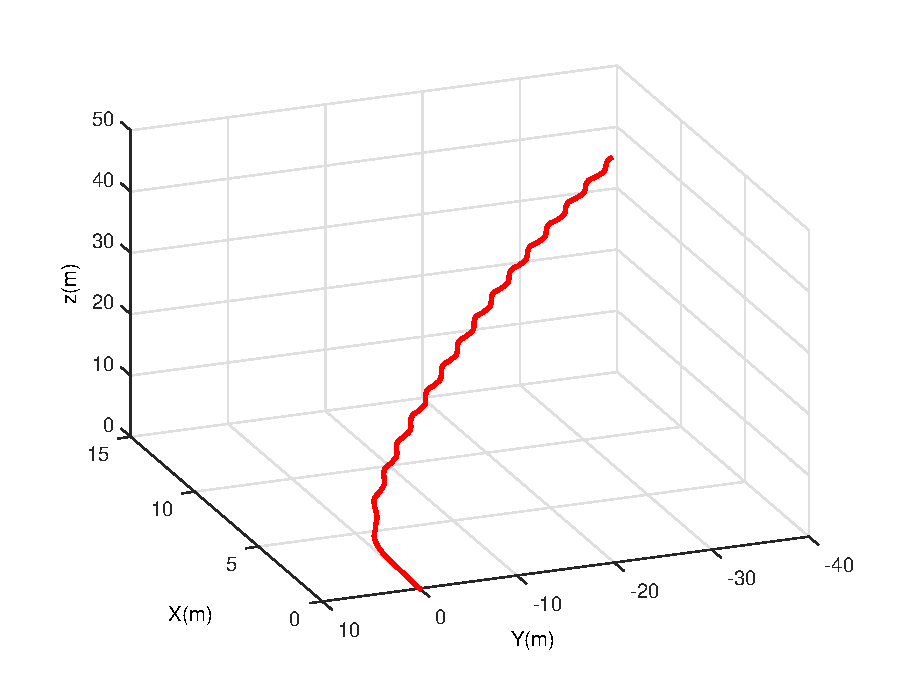
\includegraphics[width=10cm]{figure/chap3/trajectory_anlge_10_u_2.eps}
\label{fig:chap3:F3}
\bicaption[fig:chap3:F3]{AUV的3D运行轨迹}{AUV的3D运行轨迹} {Fig.}{AUV's trajectory on 3-D plot}
\end{figure}

从数值实验获得的测量数据是每个自由度中AUV的速度值。 然而,目标函数是从REMUS AUV的数学模型中推到出的,其包含符号回归中实用的加速度。 为了提高计算速度和便于搜索最优解,使用方程\ref{eq:chap3:13}中描述的欧拉数值方法来获取每个时刻加速度值。 此外,在实际测量中获得的数据主要是速度或加速度的状态数据的一部分,这对于参数辨识并不够。 也可以通过适当地使用欧拉数值方法获得所有必要的状态数据以方便进行参数辨识。

\begin{equation}
\begin{array}{l}
\label{eq:chap3:13}
 \dot u\left( k \right) = \left[ {u\left( {k + 1} \right) - u\left( k \right)} \right]/h \\
 \dot v\left( k \right) = \left[ {v\left( {k + 1} \right) - v\left( k \right)} \right]/h \\
 \dot w\left( k \right) = \left[ {w\left( {k + 1} \right) - w\left( k \right)} \right]/h \\
 \dot p\left( k \right) = \left[ {p\left( {k + 1} \right) - p\left( k \right)} \right]/h \\
 \dot q\left( k \right) = \left[ {p\left( {k + 1} \right) - p\left( k \right)} \right]/h \\
 \dot r\left( k \right) = \left[ {r\left( {k + 1} \right) - r\left( k \right)} \right]/h \\
 \end{array}
 \end{equation}
其中, $h$ 是采样的时间间隔。

使用Levenberg-Marquardt方法来估计具有已知非线性结构的水下机器人模型的参数。 方法是使用MATLAB中使用优化工具箱实现的,LM方法的设置条件如下:TolFun为1e-8,迭代最大次数为800,每个参数的上下边界为-2000到200。

\begin{figure}[!htp]
\centering
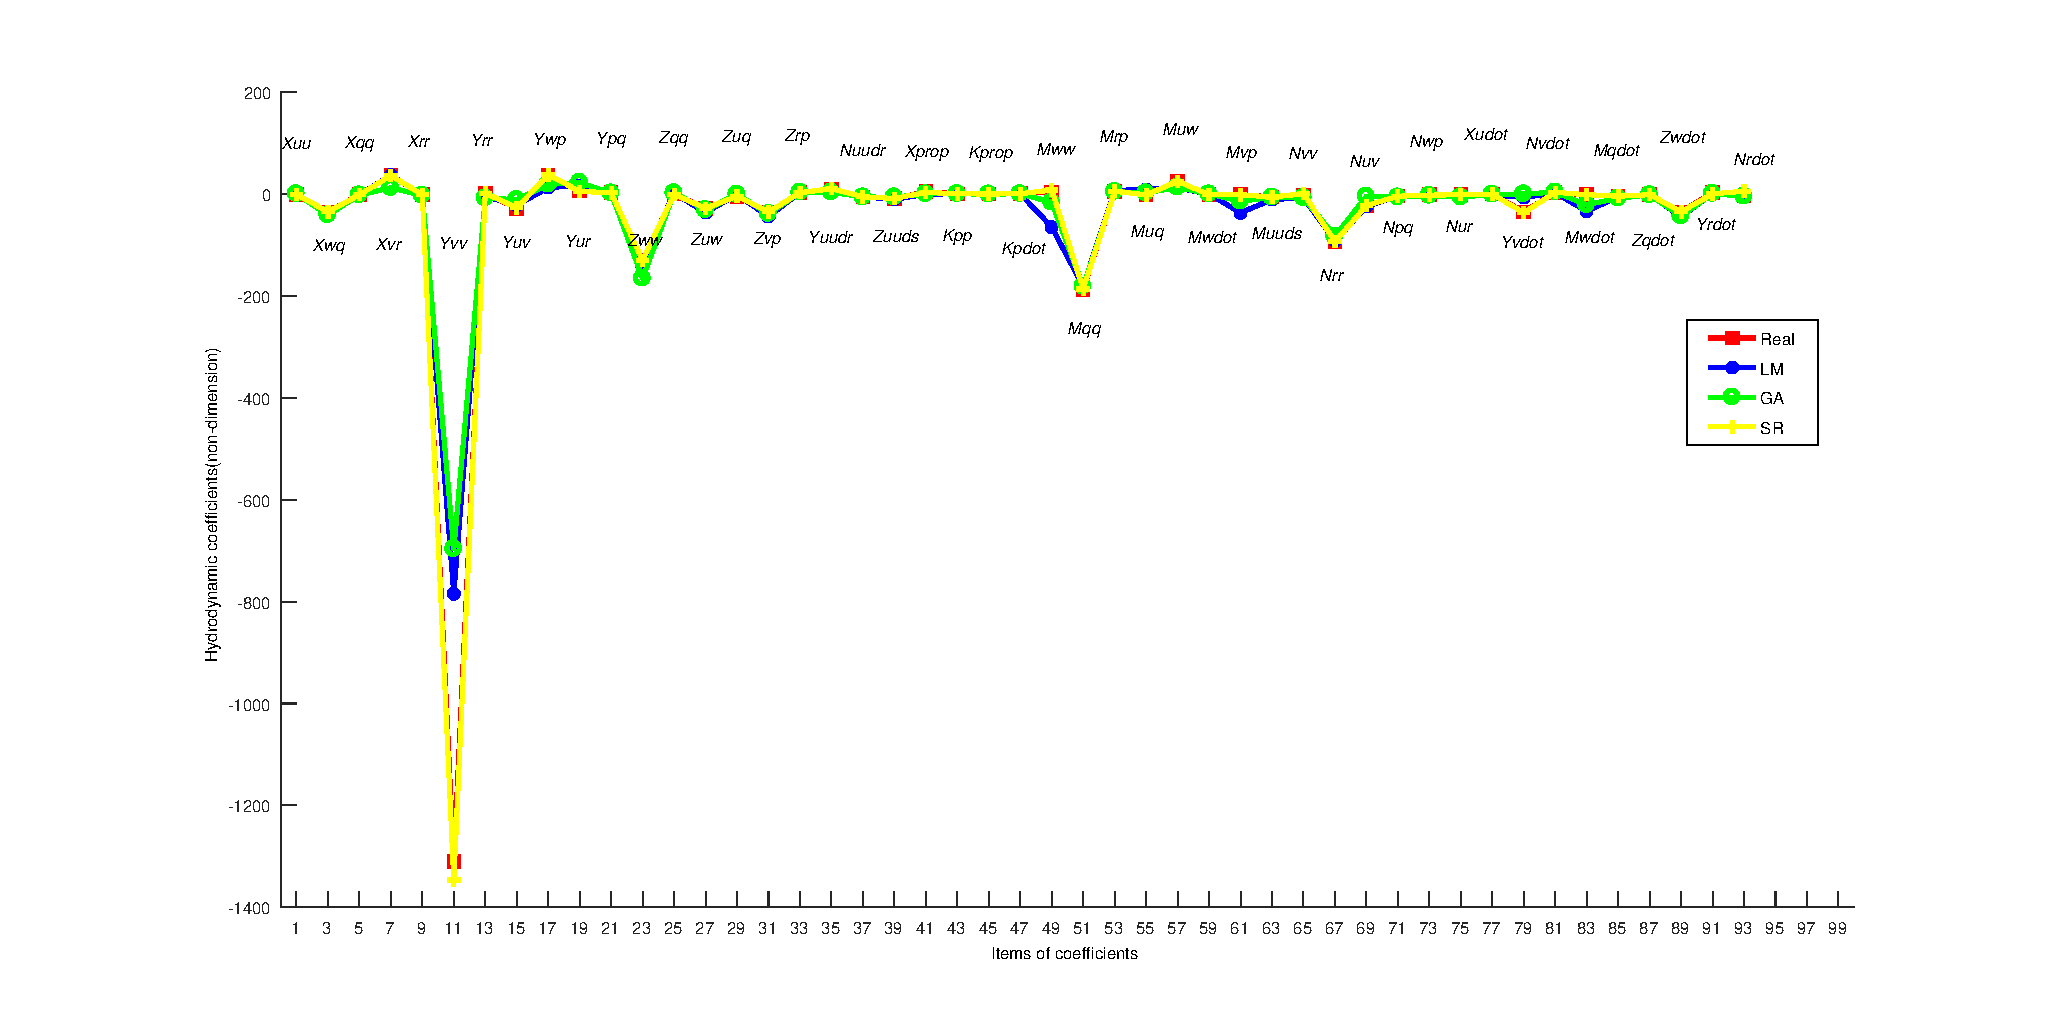
\includegraphics[width=1\textwidth]{figure/chap3/four_full.eps}
\label{fig:chap3:F4}
\bicaption[fig:chap3:F4]{使用LM、GA、SR方法进行AUV水动力参数辨识性能总体对比}{使用LM、GA、SR方法进行AUV水动力参数辨识性能对比} {Fig.}{AUV hydrodynamic coefficients comparisons between LM, GA, SR and Real Model}
\end{figure}

\begin{figure}[!htp]
\centering
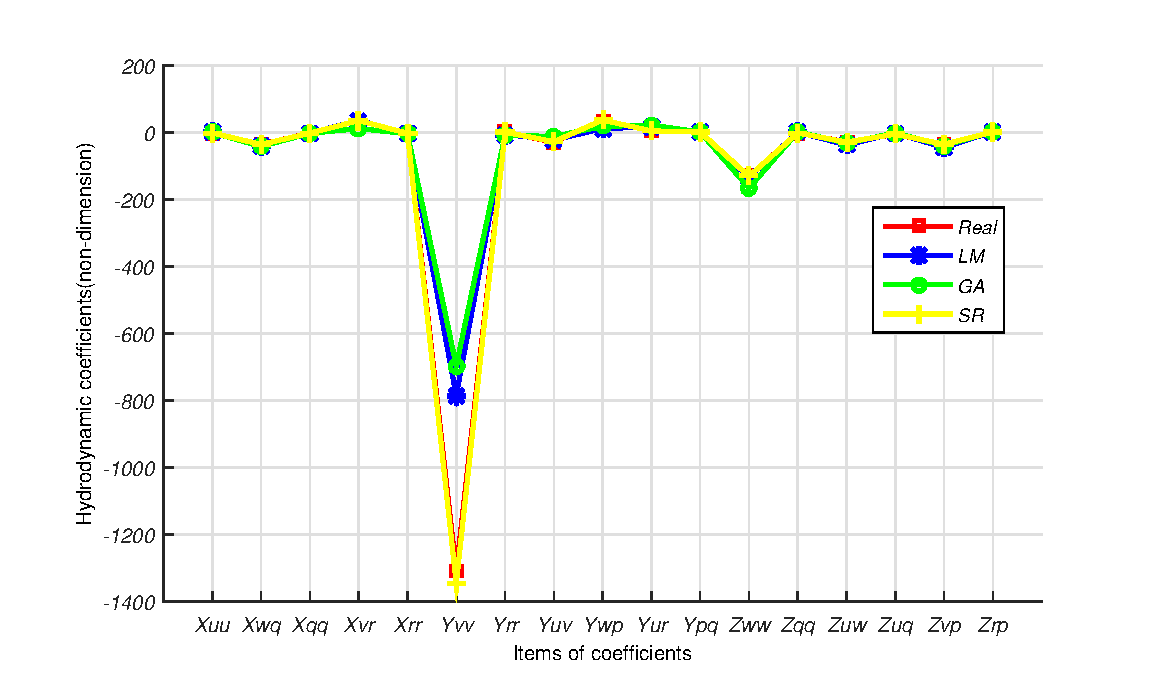
\includegraphics[width=14cm]{figure/chap3/four_1_17.eps}
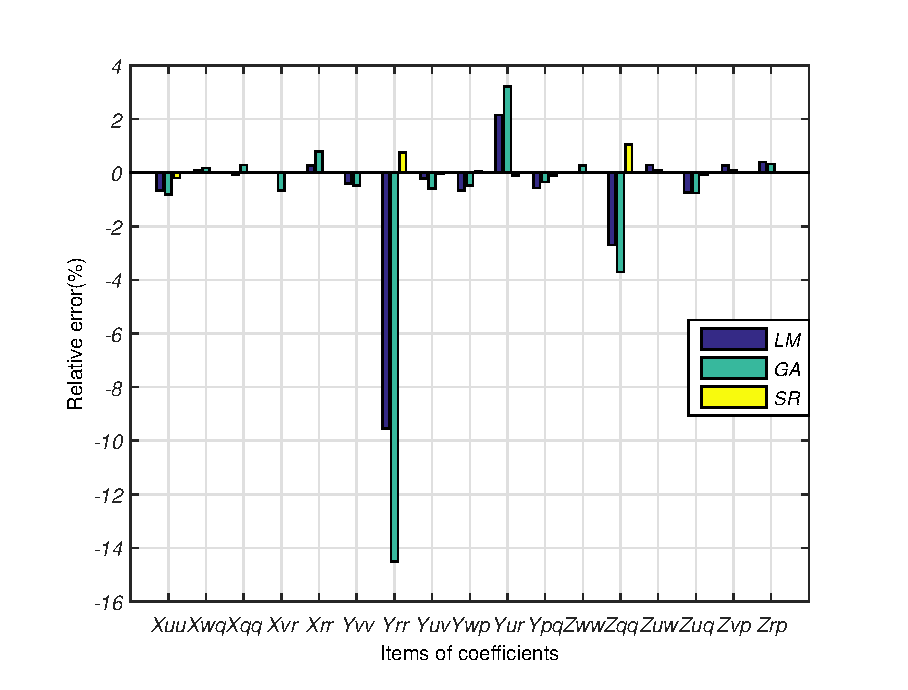
\includegraphics[width=14cm]{figure/chap3/relative_error_1_17.eps}
\label{fig:chap3:F5}
\bicaption[fig:chap3:F5]{使用LM、GA、SR方法进行AUV水动力参数辨识性能对比(1-17参数)}{使用LM、GA、SR方法进行AUV水动力参数辨识性能对比(1-17参数)} {Fig.}{AUV hydrodynamic coefficients comparisons between LM, GA, SR and Real Model(1-17)}
\end{figure}

\begin{figure}[!htp]
\centering
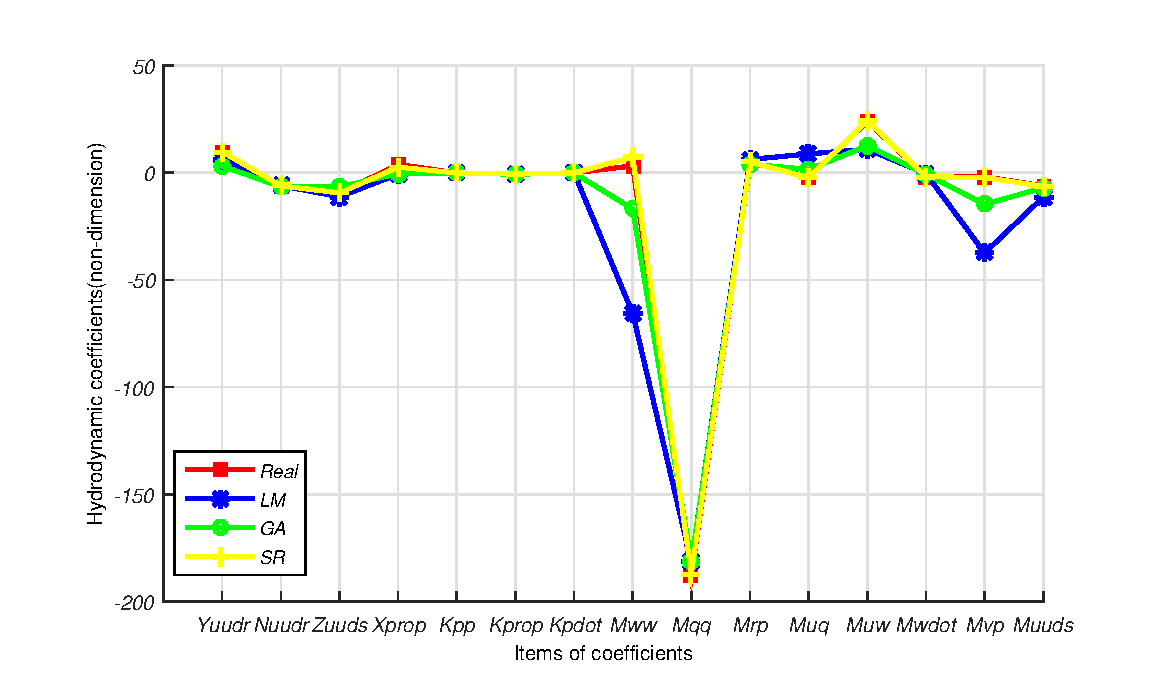
\includegraphics[width=14cm]{figure/chap3/four_18_32.eps}
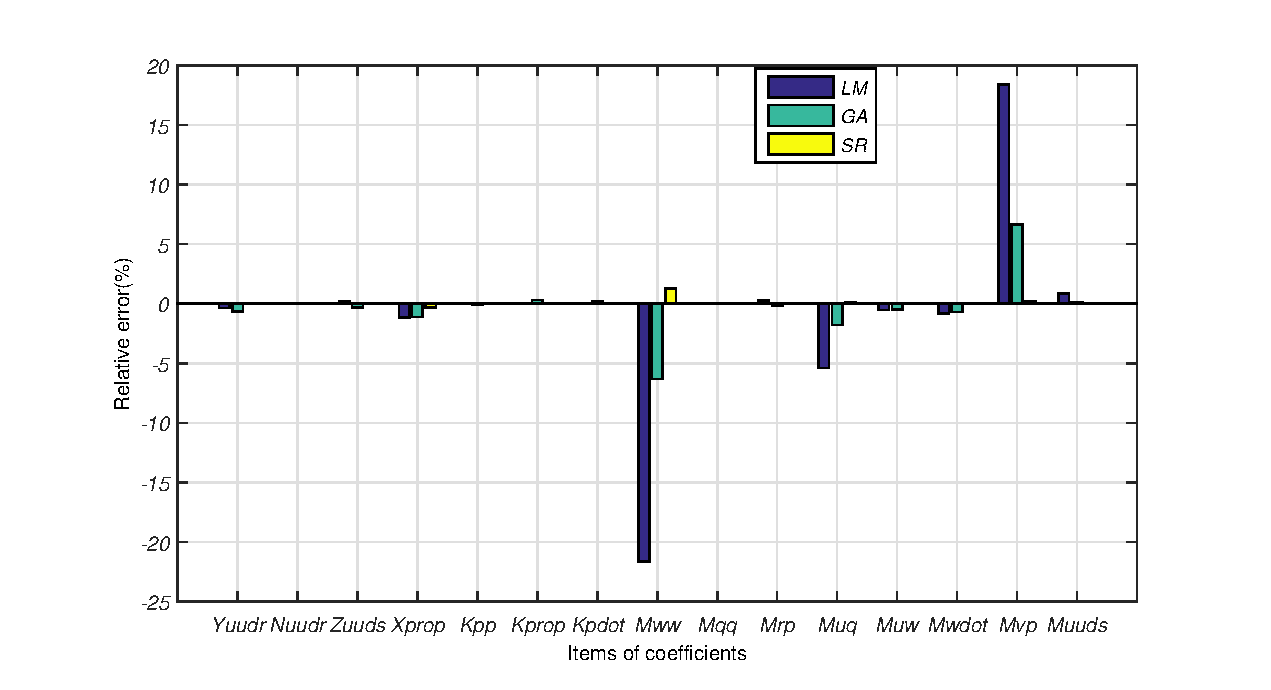
\includegraphics[width=14cm]{figure/chap3/relative_error_18_32_.eps}
\label{fig:chap3:F6}
\bicaption[fig:chap3:F6]{使用LM、GA、SR方法进行AUV水动力参数辨识性能对比(18-32参数)}{使用LM、GA、SR方法进行AUV水动力参数辨识性能对比(18-32参数)} {Fig.}{AUV hydrodynamic coefficients comparisons between LM, GA, SR and Real Model(18-32)}
\end{figure}

\begin{figure}[!htp]
\centering
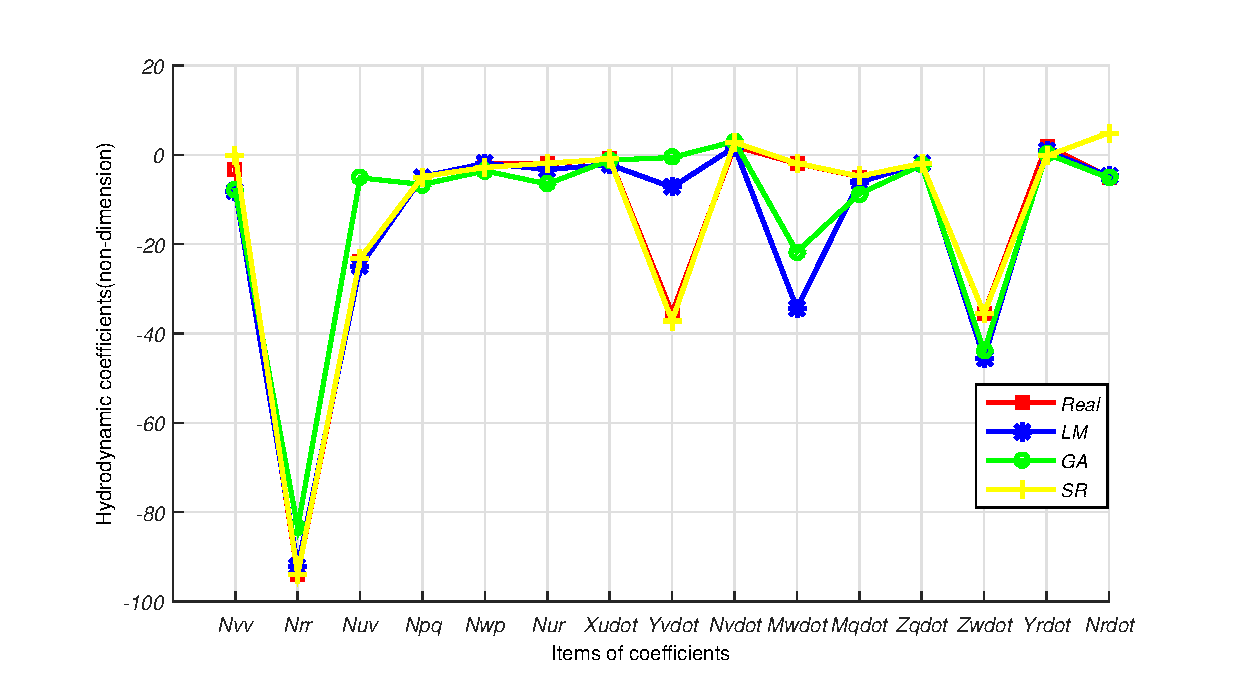
\includegraphics[width=14cm]{figure/chap3/four_33_47.eps}
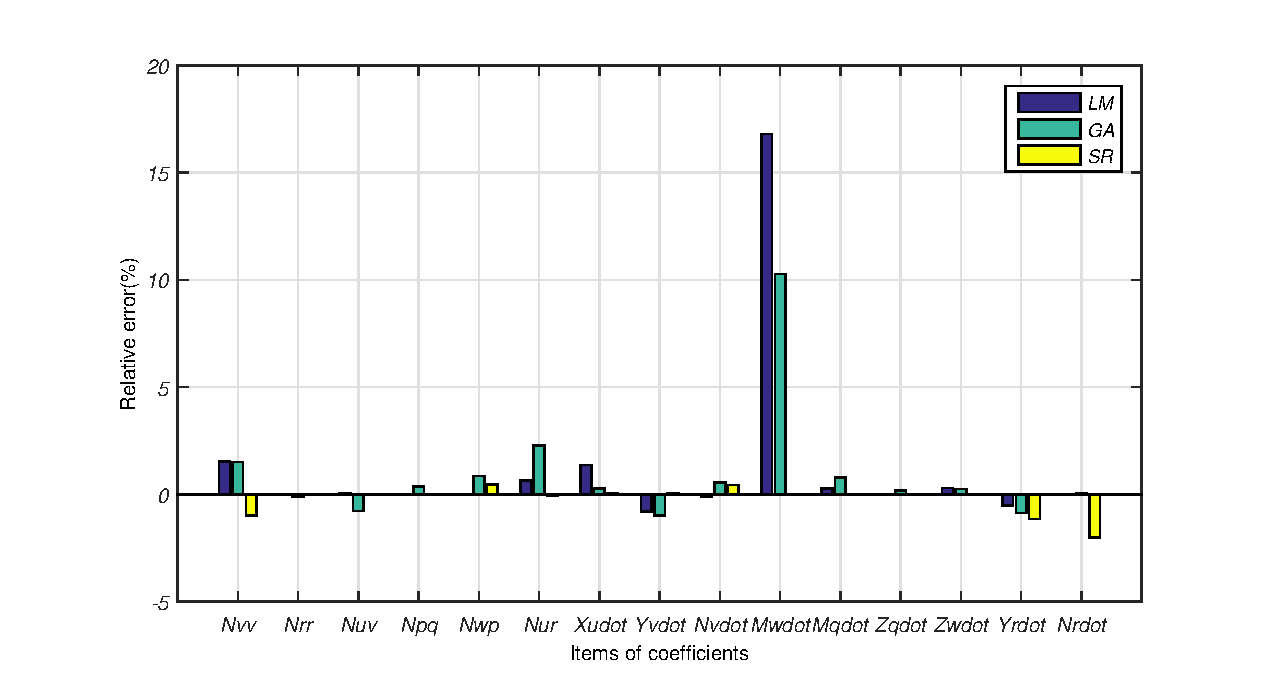
\includegraphics[width=14cm]{figure/chap3/relative_error_33_47.eps}
\label{fig:chap3:F7}
\bicaption[fig:chap3:F7]{使用LM、GA、SR方法进行AUV水动力参数辨识性能对比(33-47参数)}{使用LM、GA、SR方法进行AUV水动力参数辨识性能对比(33-47参数)} {Fig.}{AUV hydrodynamic coefficients comparisons between LM, GA, SR and Real Model(33-47)}
\end{figure}

遗传算法也可以识别水下航行器的参数,但搜索范围应适当地设置。 为了获得参数估计的良好结果, 最大遗传代数, 种群规模,交叉和变异概率分别为500, 80, 0.7, 0.02。

C. 参数辨识结果对比

图\ref{fig:chap3:F4} 将LM,GA,SR的辨识结果与实际模型系数进行比较。辨识的流体动力学系数基本上与模型的实际参数吻合良好;然而,对于一些系数,使用GA和LM算法估计的参数数值与实际参数数值相比,差异较大。 GA在一定程度上改善了水动力参数(如$Mww$,$Muq$,$Mvp$,$Mwdot$,$Zwdot$)的估计效果,但根据用于评估GA的参数识别的总体性能表\ref{tab:chap3:table1}中的MSE和STD的计算结果与使用LM方法相比,两者没有太大差异。此外,GA的搜索范围由LM的计算结果确定的,GA估计的过程非常耗时,而LM和SR更高效、计算更快,因为他们从开始估计的 100 秒内误差就收敛到一个很小的范围内。只不过, LM方法,由于会存在落入局部最优解的可能,容易在一次性搜索的过程中失败。对于符号回归方法,所有系数都是在选取数据集的50%和50%的情况下进行的模型训练和测试,这可以保持提出的方法的有效性。通过设置AUV的六个目标方程来确定所有参数。在图\ref{fig:chap3:F4}中的 $Yvv$ (也可见图\ref{fig:chap3:F5})和 $Yvdot$ (也可见图\ref{fig:chap3:F7})中显示出良好的一致性,其中 $dot$表示每个速度的导数。SR估计的模型参数的相对误差远小于由GA和LM识别的模型参数的相对误差,这说明了SR方法具有良好的参数识别能力。

\begin{table}[!t]
  \centering
  \label{tab:chap3:table1}%
  \bicaption[tab:chap3:table1]{LM, GA, SR方法的MSE和STD结果对比}{LM, GA, SR方法的MSE和STD结果对比}{Table}{Comparisons of MSE and STD between LM, GA and SR}
  \begin{tabular}{cccc}
  \toprule
        & MSE         & STD     & Processing time  \\
  \midrule
    LM  & 6.0645e+03  & 78.3369 & 33min            \\
    GA  & 8.1315e+03  & 90.4354 & 2h               \\
    SR  & 31.1485     & 5.6254  & 16min8s          \\
  \bottomrule
  \end{tabular}%
\end{table}%


为了进一步研究噪声对搜索过程的影响,根据收敛和参数辨识的效果,选择使用SR和LM方法来识别不同信噪比SNR传感器采集的带噪声运动数据。

如表\ref{tab:chap3:table2}所示,MSE和STD是LM方法识别的模型系数和实际力系数比较的评价标准,而最大误差,MSE和MAE是SR方法的收敛性评价标准; 在实验中,随着SNR的值的增大,两种方法都实现了收敛过程速度的显着提高,这里设定的条件是LM和SR的搜索时间均为8分钟; 而由于传感器质量的差异,传感器的质量越差,通过将识别结果进行比较,发现LM方法辨识的结果的性能评估标准会变得数值较大。

\begin{table}[!t]
\centering
\label{tab:chap3:table2}
\bicaption[tab:chap3:table2]{不同SNR模型数据的辨识效果对比}{不同SNR模型数据的辨识效果对比}{Table}{Evaluation of identification results and measured performance along with SNR}
\begin{tabular}{ccccccc}
\toprule
                       & SNR   &       1   & 10       & 20       & 45       & No noise \\
\midrule
\multirow{2}{*}{LM}    & MSE   & 194235    & 115055   &53575     &21412     &17937      \\
                       & STD   & 438.0196  & 333.6798 &227.4539  &  145.9737  &  132.549  \\
\midrule
\multirow{3}{*}{SR}    & Maximum Error & 49.9913 &19.06  & 6.4719  &0.4098 & 0.0118      \\
                       & MSE           & 227.2457  &  38.49  & 3.7726 & 0.0127 & 1.39E-05 \\
                       & MAE           & 12.1192& 4.9485  &1.5513  &0.089  & 0.0027        \\
\bottomrule
\end{tabular}
\end{table}

此外,为了验证SR在处理非连续数据方面的优势,我们将具有SNR等于45的相同测量运动数据放在一起,并重复使用SR方法进行参数识别。 在100秒内,SR目标函数的MAE仍收敛于小于0.1的值,最后经过20min17sec后得到MAE = 0.00136003,MSE = 0.0000036257619的结果。 REMUS第一自由度纵荡运动的流体力学系数的搜索结果如表\ref{tab:chap3:table3}所示。此外,我们还从各种运动状态数据集中随机选择数据构成新的辨识数据集,然后获得了REMUS模型的参数,这说明SR方法不仅 具有良好的收敛性,也可以获得更加准确的参数识别结果。同样也说明使用非连续数据集进行水动力系数识别SR方法也表现出出色的性能。

\begin{table}
\centering
\label{tab:chap3:table3}
\bicaption[tab:chap3:table3]{非连续数据集的符号回归辨识}{非连续数据集的符号回归辨识}{Table}{Identification parameters using noncontinuous motion data with SR}
\begin{tabular}{cccc}
\toprule
             &Real coefficients & Steering angle is same & Random Selected data\\
\midrule
 $X_{uu}$    & -1.62 &-1.620937076   & -1.606133018 \\
 $X_{\dot u} $   &-0.93  &-0.951148025   & -0.644722161 \\
 $X_{wq}$    &-35.5  & -35.53024222  & -34.85176751  \\
 $X_{qq}$    &-1.93  &  1.939137984  &1.953199585   \\
 $X_{vr}$    &35.5   & 35.53904256   &34.83378219  \\
 $X_{rr}$    &-1.93  &  -1.935145734 &-1.925233784  \\
 $X_{prop}$    &3.86   & 3.861580558   &3.919602871  \\
\bottomrule
\end{tabular}
\end{table}

如表 \ref{tab:chap3:table4}所示,使用Eureqa软件进行了水下航行器功能结构形式的搜索测试,这有助于研究者为REMUS AUV 的纵荡自由度运动找到一些有用的新的表达形式的模型,并给出模型的外力的表达形式,这对于确定水下机器人的简化数学模型非常有帮助。

在图\ref{fig:chap3:F8}和表\ref{tab:chap3:table4}中,给出了不同于非线性模型的外部力的新的表达形式,这是使用结构搜索发现的模型的另一种简化表达。AUV的受到的实际力和简化模型的估计的力之间的预测值是一致的,并且具有稳定性,这表明了所提出的方法适合用于模型的结构搜索。

\begin{table}
\centering
\label{tab:chap3:table4}
\bicaption[tab:chap3:table4]{AUV模型的结构搜索}{AUV模型的结构搜索}{Table}{Structure searching for AUV model}
\begin{tabular}{cc}
\toprule
Target expression & $\begin{array}{l}
 \dot u = {f_1}\left( {u,v,w,p,q,r,\dot v,\dot w,\dot p,\dot q,\dot r,delt{a_s},{\mathop{\rm de}\nolimits} lt{a_r}} \right) \\
  + {f_2}\sin \left( {theta} \right) \\
 \end{array}$  \\
\midrule
Function sets  & Constant,+,- ,*,/,abs() \\
\tabincell{c}{Search function \\ modal for surge} & $\begin{array}{l}
 \dot u = 2.45vr + 0.0342\sin (theata) - 2.2255wq \\
  - 0.1560q\^3 - 0.3914 \\
 \end{array}$ \\
\tabincell{c}{Search for external forces \\in the freedom of sway} & $\sum {FY}  = 3.3217 + 15.6577ur - 753.4552v\left| v \right|$ \\
\bottomrule
\end{tabular}
\end{table}

\begin{figure}[!htp]
\centering
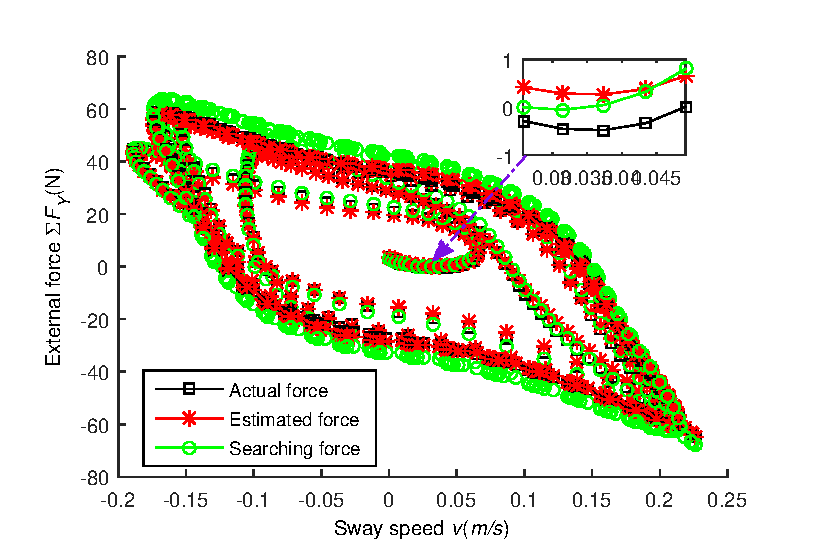
\includegraphics[width=14cm]{figure/chap3/search_compare.eps}
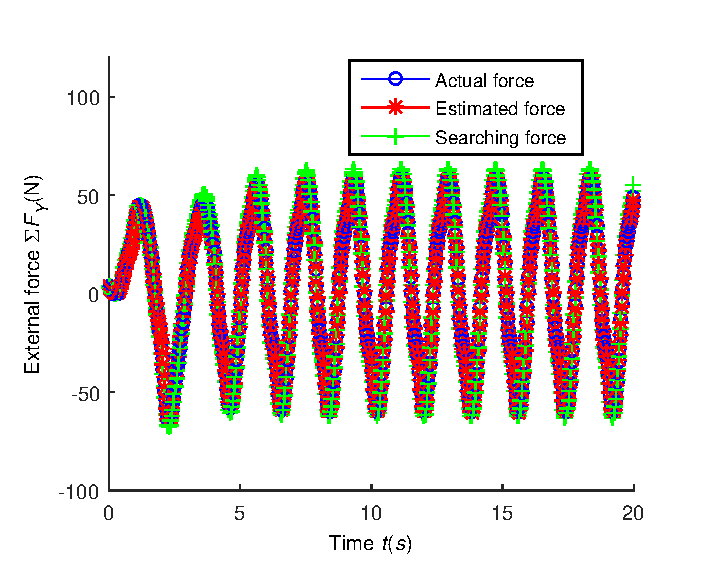
\includegraphics[width=14cm]{figure/chap3/time-force_compare.eps}
\label{fig:chap3:F8}
\bicaption[fig:chap3:F8]{实际、估计与搜索的外部力对比}{实际、估计与搜索的外部力对比} {Fig.}{comparisons of AUV external force on sway freedom between Actual, Estimated and Searching forces}
\end{figure}

在本节中,已经使用多种方法辨识和搜索了AUV模型的参数和结构。将模型的实际阻尼系数的值用作真值,然后与估计值进行比较。 非线性模型的辨识效果是使用LM算法、遗传算法和基于遗传编程的符号回归三种方法进行估计,并得到了水动力学模型参数。此外,还讨论并确认了传感器模型的影响以及符号回归方法的优点。最后,使用符号回归方法搜索AUV的模型结构。 结果表明,符号回归可以比LM和GA方法更准确地确定非线性模型的模型参数,并且还可以搜索数据集以获得AUV模型的表达形式,可以发现新表达形式。 因此,符号回归更适用于AUV系统建模。


\section{水流环境识别 }

水下航行器工作的水下环境对于其能够正常工作和作业至关重要,尤其是深海环境中存在的水流环境,本节主要研究
AUV型的水下机器人在水流环境中的感知问题\cite{verschure2003environmentally,fossen1994guidance}。首先介绍从鱼类生物学启发感知中找寻到研究灵感,发现鱼体侧线因受到水流变化而产生的神经冲动,不断地刺激鱼类的前端神经和大脑,使得鱼类可以感知水流的方向,利用水中存在能量完成巡游。其次,神经脉冲信号处理的过程类似于一个从大量数据学习水流模式的过程\cite{abdulsadda2013underwater,abdulsadda2012artificial,yang2010artificial,ren2012model}。典型的机器学习可以用来训练用于区分水流模式的模型\cite{liu2012support}。不过,应当考虑大规模传感器数据的信息稀疏特性,对其进行预处理\cite{chen2000new}。压缩感知可以用来处理大量的传感器数据,而能代表数据最大特性的一般就是其带有分类特性的特征向量。线性判别分析是一类可以压缩高维数据并带有分类特性的处理方法,因此本章将采用线性判别分析对数据进行预处理\cite{chen2000new,martis2013ecg}。最后,为了选择出保持分类的高正确率的分类器,选择使用了支持向量机,并对比多种内核的特性,训练出水流模型的方向分类器,并进行测试。

\subsection{鱼类侧线感知系统 }

鱼类拥有一个能够对周围水下环境感知运动的微机械感应侧线系统。它分布于鱼皮肤的两侧,主要由神经丘和侧线管组成(图\ref{fig:chap3:F9}与\ref{fig:chap3:F10})。神经丘体位于鱼体表皮上并向外凸起,使得它能够侵润到外部流体中,侧线管组成了侧线系统的大部分,每隔一个微小距离就通过侧线孔与外界流场相连。外部流体通过侧线管中液体的流动可以将流场中水内外声波,压力,水流速度改变信息传递给神经丘,神经丘的感觉神经细胞受到刺激通过神经纤维,经侧线神经传递到鱼的大脑。

    \begin{figure}[!htp]
    \centering
        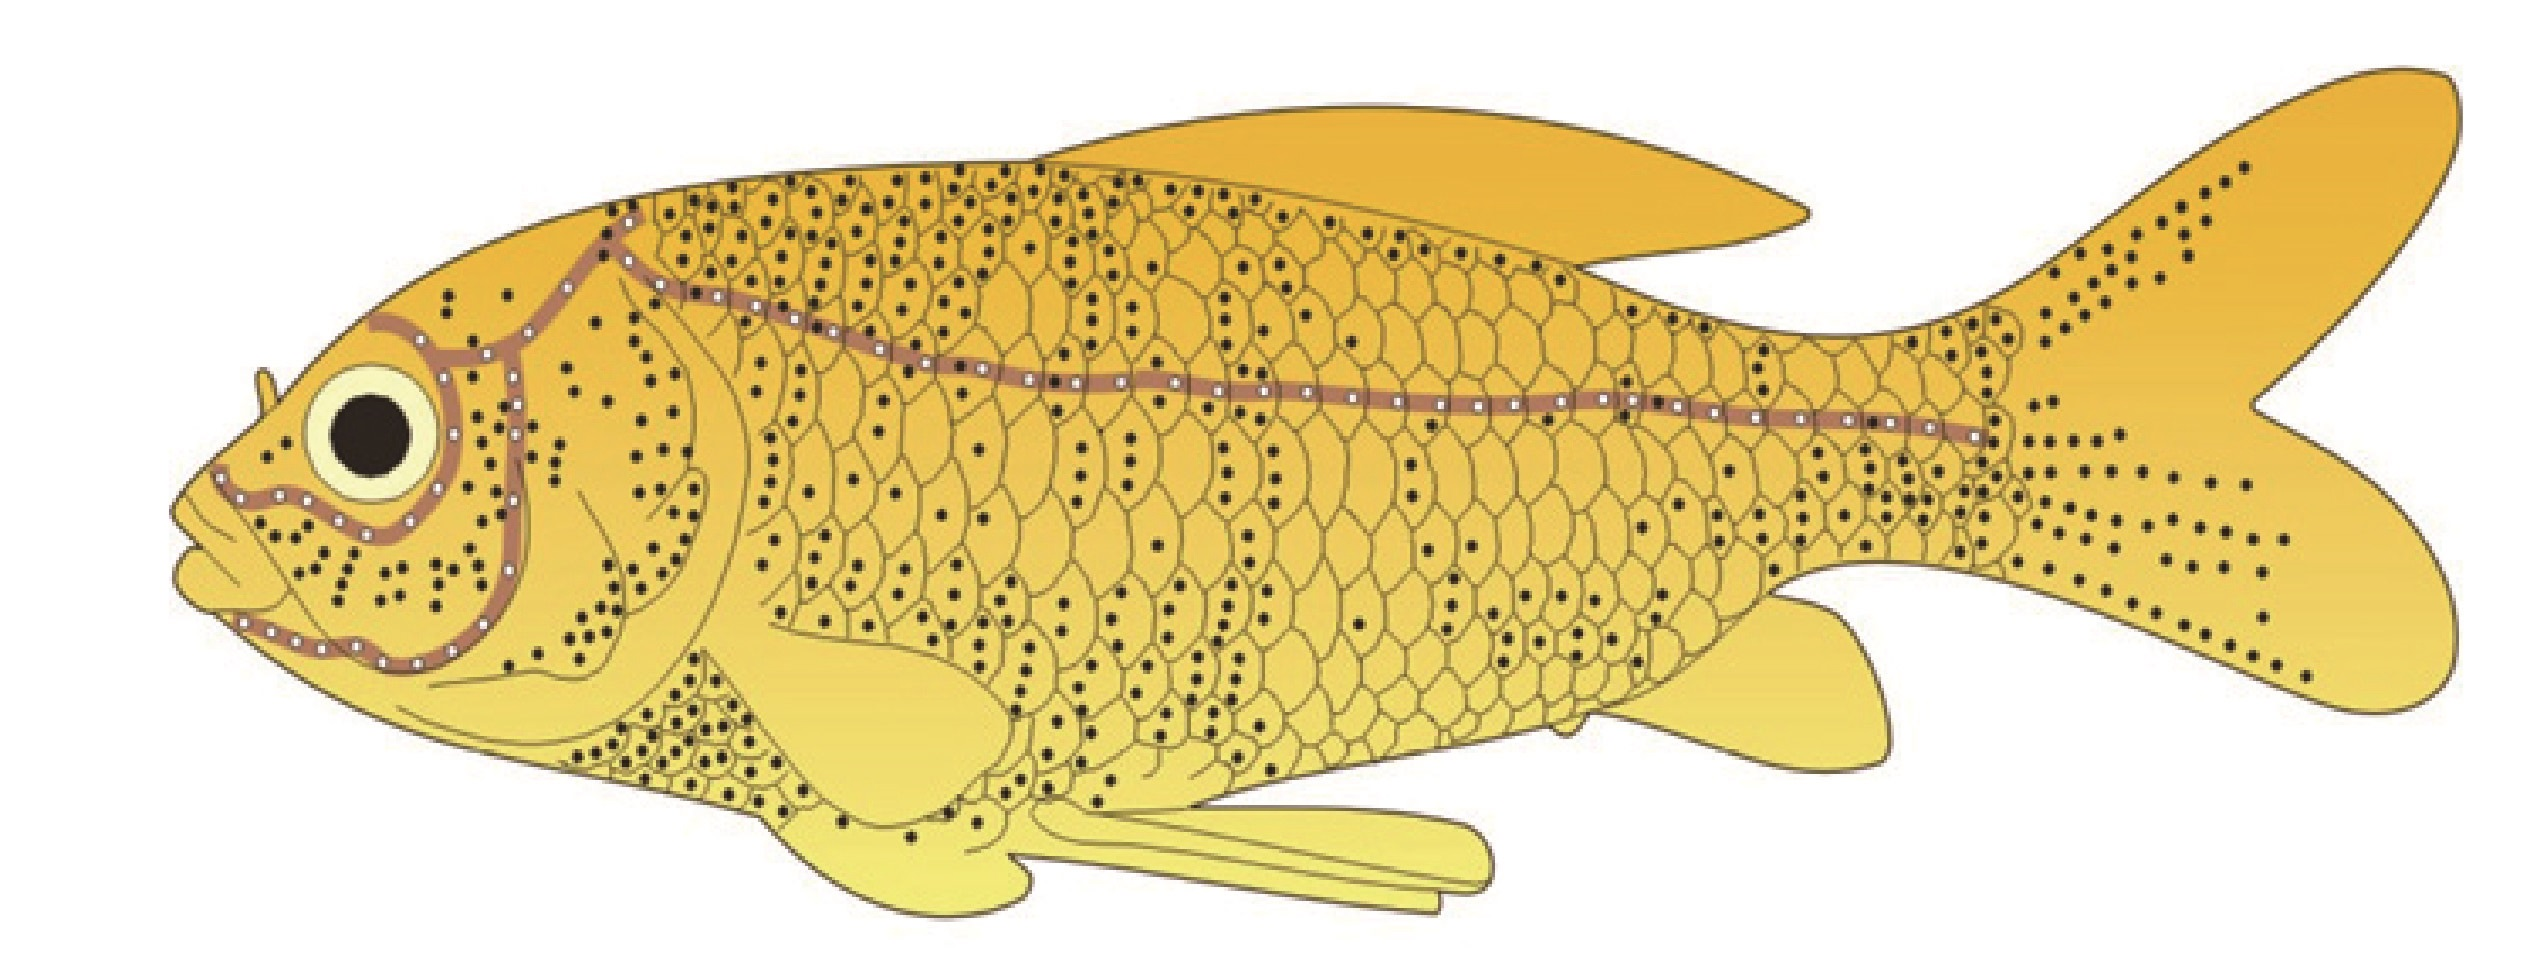
\includegraphics[width=11cm]{figure/chap3/fig1.jpg}
        \label{fig:chap3:F9}
        \bicaption[fig:chap3:F9]{鱼体侧线位置示意(棕色线)}{鱼体侧线位置示意(棕色线)} {Fig.}{Location of fish lateral line system(Brown)\cite{abdulsadda2012artificial} }
    \end{figure}

    \begin{figure}[!htp]
    \centering
        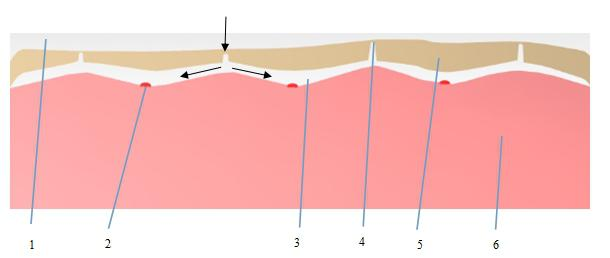
\includegraphics[width=14cm]{figure/chap3/fig2.jpg}
        \label{fig:chap3:F10}
        \bicaption[fig:chap3:F10]{鱼侧线局部放大示意图}{鱼侧线局部放大示意图:$1$ 水 $2$ 神经丘 $3$ 侧线管 $4$ 侧线孔 $5$ 表皮 $6$ 真皮} {Fig.}{enlarged partial schematic of fish lateral line:$1$ Water $2$  Neuromast  $3$ Lateral line tubes $4$ Lateral line pores $5$ Epidermis 6 Dermis  }
    \end{figure}

\subsection{基于支持向量机的水下机器人水流环境辨识  }

\subsubsection{流体控制方程 }
建立的模型是为了求解AUV本体周围的水流问题,用以提取二维面内的侧线节点压力数据。该模型是基于雷诺平均纳维-斯托克斯(Reynolds Averaged Navier–Stokes,RANS)方程。 对于湍流情况,速度场和水流场能够划分为两个部分:均值速度$<u_{i}>$ 与压力 $<p_{i}>$ , 湍流速度 $u_{i}^{'}$ 与压力 $p_{i}^{'}$。 这样 $u_{i} =  < u_{i} >  + u_{i}^{'}$ ,$p_{i} =< p_{i} >+p_{i}^{'}$,其中二维流分析 $i=1, 2$。如果流体假设是不可以压缩的,那么平均水流场主要是有RANS方程的情况:
\begin{equation}
\label{eq:chap3:14}
\frac{{\partial {U_j}}}{{\partial {x_j}}} = 0
\end{equation}

\begin{equation}
\label{eq:chap3:15}
\frac{{\partial {U_i}}}{{\partial t}} + \frac{\partial }{{\partial {x_j}}}\left( {{U_i}{U_j}} \right) = \frac{1}{\rho }\frac{{\partial P}}{{\partial {x_j}}}\left( {{\Gamma _{ij}} - \rho \bar u_i^{'}\bar u_j^{'}} \right)
\end{equation}
其中,$\rho$是流体密度,雷诺应力张量为\\

\begin{equation}
\label{eq:chap3:16}
 - \rho {{\bar u_i}^{'}}{{\bar u_j}^{'}} = \left[ {\begin{array}{*{20}{c}}
   { - \rho \bar u{{_1^{'}}^2}} & { - \rho {\bar u_1^{'}}{\bar u_2^{'}}}  \\
   { - \rho {\bar u_2^{'}}{\bar u_1^{'}}} & { - \rho \bar u{{_2^{'}}^2}}  \\
\end{array}} \right]
\end{equation}

$k-\varepsilon$ 模型是一种外部空气和流体动力学应用最广泛的湍流模型\cite{lamb1932hydrodynamics}。 因此文中选用其作为模拟航行器周表压力的湍流模型。

$k$函数\\

\begin{equation}
\label{eq:chap3:17}
\frac{{\partial \rho k}}{{\partial t}} + \nabla \left( {\rho \bar Uk} \right) = \nabla \left[ {\left( {\mu  + \frac{{{\mu _t}}}{{{\sigma _k}}}} \right)\nabla k} \right] + {P_k} - \rho \varepsilon
\end{equation}

$\varepsilon$函数\\

\begin{equation}
\label{eq:chap3:18}
\frac{{\partial \rho \varepsilon }}{{\partial t}} + \nabla \left( {\rho \bar U\varepsilon } \right) = \nabla \left[ {\left( {\mu  + \frac{{{\mu _t}}}{{{\sigma _k}}}} \right)\nabla \varepsilon } \right] + \frac{\varepsilon }{k}\left( {{C_{\varepsilon 1}}{P_k} - {C_{\varepsilon 2}}\rho \varepsilon } \right)\end{equation}

其中,\[{P_k} = {\mu _t}\nabla \bar U \left( {\nabla \bar U + \nabla {{\bar U}^T}} \right) - \frac{2}{3}\nabla {\bar U} \left[ \left( {3{\mu _t}\nabla } \bar U   + \rho k   \right)\right] \]

\[{\mu _t} = {C_\mu }\rho \frac{{{k^2}}}{\varepsilon }\]

文节研究的对象是一个鱼雷型AUV,模仿REMUS AUV 设计而成,它能够工作在水深100m区域并进行多项任务。整个模型是长圆柱型并有四个舵在尾部,其中有两个水平舵,两个垂直舵。关于体坐标系的Oxy 面和Oxz面对
称,因此AUV 运行分析的流体域简化为二维平面
流体域。整个计算模型是使用ICEM软件建立的1:1的网格模型。网格主要是三角型网格,网格节点数为18253。网格划分可以见图\ref{fig:chap3:F11}。流体域是个圆形水域,直径为15m,左侧为来流入口,右侧围出口,内部为AUV外边界,内边界根据AUV水下运动的特性为O型网格。

边界层设置:边界层的设置在ICEM和Fluent中完成,包括(1)流体域左半圆边界,流体域右半圆边界,因为来流方向是 $0, 45, 90, 135, 180, 225, 270,315$八个主要方向进行计算,入口出口的设置根据来流方向进行调整并设置不同的来流速度大小($0-3 m/s$);(2)内部边界是AUV的侧线提取数据边界,设为wall, 流体域为FLUID。 因为海中的深水水流主要是稳定的, 因此本次只进行稳定流场的计算。其中计算结果如图\ref{fig:chap3:F12}所示。

    \begin{figure}[!htp]
    \centering
        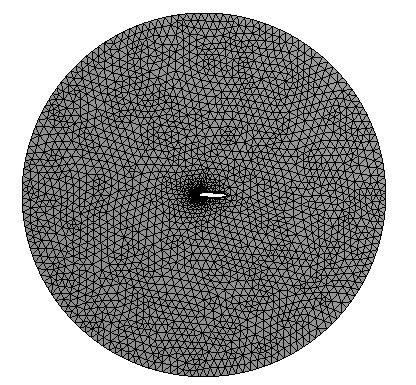
\includegraphics[width=10cm]{figure/chap3/fig4.jpg}
        \label{fig:chap3:F11}
        \bicaption[fig:chap3:F11]{流体网格模型}{流体网格模型} {Fig.}{Fluid mesh }
    \end{figure}

    \begin{figure}[!htp]
    \centering
        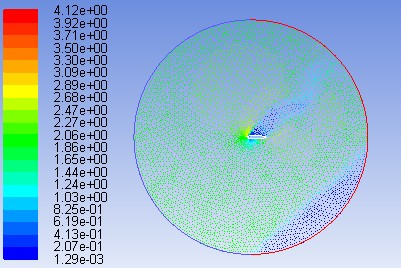
\includegraphics[width=13cm]{figure/chap3/fig5.jpg}
        \label{fig:chap3:F12}
        \bicaption[fig:chap3:F12]{45度水流计算流速图}{45度水流计算流速图} {Fig.}{Velocity profile for vehicle with 45 degree inflow }
    \end{figure}

\subsubsection{ 水流识别方法 }

水流的识别主要需要确定两个基本要素,即水流的方向和流速的大小。而建立水流预测模型要能够对这两点进行正确地估计。由于提取的压力数据节点较多,使用分类器直接训练,计算成本较高。而传感器数据的信息是稀疏分布的,有重要的,有不重要的。为了提取出来重要的数据特征信息,线性判别分析方法被用来处理压力传感器数据,并得到了很多代表流向特征的数据信息。将获得的特征信息输入到支持向量机建立的水流方向分类器里面,对分类器进行训练。在确定了水流的流向后,仍然有一个重要的要素需要注意,那就是水流的流速大小。要辨别流速大小并不容易,尤其是当水流的速度值较小的时候,因此使用拟合法来建立水流流速的预测方程,输入到方程里的是压力极值,输出是流速。如此就可以完成对水流的流速方向和大小的模式预测。并且,预测的处理也参考了鱼的层级处理结构\cite{yang2010artificial}。

A. {线性判别分析}

线性判别分析({Linear Discriminant Analysis})是一种监督式的机器学习方法,这种方法不是使用概率知识来训练和预测数据的模式的,因此线性判别分析并不需要关于数据的已知的先验和后验概率值。线性判别分析的主要思想是将输入的高维度的数据投影到一个较低的维度空间内。在这个空间中,数据的点将被划分为一个个的簇,并且这些簇之间保持一定的距离。这里提到簇就是所说的类的低维度空间的表示。线性判别分析采用的投影处理,可以让高维度的压力数据降低维度,并保持较好的分类特性,这是该方法的优点。下面将给出线性判别分析的主要理论。

线性判别分析从其名字就可以知道该方法属于线性分类器。这种分类器具有 $k$线性函数,而这些函数都是为了所需要划分的$K$类问题而定义。协方差矩阵被定义如下\cite{martis2013ecg,chen2000new}:

\begin{equation}
{S_W} = \sum\limits_{k = 1}^K {{S_{_k}}}
\label{eq:chap3:19}
\end{equation}
其中,
\begin{equation*}
\begin{aligned}
{S_k} &= \sum\limits_{n \in {C_k}} {\left( {{x_n} - {m_k}} \right){{\left( {{x_n} - {m_k}} \right)}^T}}\\
{m_k} &= \frac{1}{{{N_k}}}\sum\limits_{n \in {C_k}} {{x_n}}
\end{aligned}
\end{equation*}
式中$N_k$ 是 $C_k$ 的模式数目,$x_n$ 是第 $n$ 种模式的观测向量。$K$是数据样本中的整体分类数,该数定义与所采集数据的水流方向有关,本文中为8。

\begin{equation}
{S_B} = \sum\limits_{k = 1}^K {{N_k}\left( {{m_k} - m} \right){{\left( {{m_k} - m} \right)}^T}}
\label{eq:chap3:20}
\end{equation}
式中,
\begin{equation*}
m = \frac{1}{N}\sum\limits_{n = 1}^N {{x_n}}  = \frac{1}{N}\sum\limits_{k = 1}^K {{N_k}{m_k}}
%\label{equation:eq5}
\end{equation*}
$m$是所有数据的平均值。

所有样本的协方差矩阵给出如下:
 \begin{equation}
{S_T} = {S_W} + {S_B}
\label{eq:chap3:21}
\end{equation}

投影矩阵的方程给出如下:
\begin{equation}
W = {\arg _W}\max \left\{ {{{\left( {W{S_W}{W^T}} \right)}^{ - 1}}\left( {W{S_W}{W^T}} \right)} \right\}
\label{eq:chap3:22}
\end{equation}

线性判别分析的系数是从投影矩阵中获得的,给出的形式如下:

\begin{equation}
y = {W^T}x
\label{eq:chap3:23}
\end{equation}
式中,$y$是线性判别分析的系数,$x$ 是给定模式下的次级区域的 $DWT$ 系数。

当满足所有条件时:如果 $j$ 无论取任何值不等式$y_k>y_j$ 都成立,那么 $x$ 就属于第 $k$ 类。根据上面的方程,就可以分别求出每一类的评估数值。根据这些评估数值,就可以对样本进行分类和数据降低维度。

B. {支持向量机 }

前面的水流流体仿真中提出的压力数据是维度很高的,如果使用分类器进行直接处理,会加大计算的成本。而基于面向载体实验和应用的目的,需要将压力数据进行处理到较低的维度内。本部分介绍的分类器所输入的数据是基于前文使用线性判别分析方法预处理过的数据。从这些数据中获得的特征向量维度低,可以反映航行器体表的压力变化情况。支持向量机(Support Vector Machine)本身属于一种二分类方法,而水流的流向确是多种多样的。要建立流向的分类器,就需要将水流方向模式的判别问题转为多个循环的标准问题来解决。支持向量机可以对数据进行泛化处理,即使数据的样本有限,也能很好判别数据的模式。因此提出的分类器选择使用支持向量机来进行整体的模式识别,下面给出支持向量机的相关理论。具体描述如下:

\begin{equation}
V = \left\{ {\left( {{x_{1,}}{y_1}} \right),...,\left( {{x_i},{y_i}} \right)} \right\}
\label{eq:chap3:24}
\end{equation}
式中,$i=1,2,\ldots$,${x_i} \in {R^n}$,${y_i} \in \left\{ { \pm 1} \right\}$。

超平面为${\omega ^T}X + b = 0$,并且 $x_i$ 是需要处理的特征向量,$y_i$ 是需要识别的模式,$\omega$ 是标准向量,$b$ 是偏差项。

支持向量机分类器的主要目的是找出一个最优的超平面,这个平面可以几乎没有错误地区分模式。经过这样的处理,最近向量到超平面间的距离就是最大的。对参数化过程进行限制,就可以得到特定的最优超平面:

\begin{equation}
\min \frac{1}{2}{\left\| {\left. \omega  \right\|} \right.^2}
\label{eq:chap3:25}
\end{equation}
\begin{equation*}
\begin{array}{*{20}{c}}
   {s.t.} & {{y_i}\left( {{\omega ^T}{x_i} + b} \right) \ge 1,\begin{array}{*{20}{c}}
   {} & {i = 1,2,...,m}  \\
\end{array}}  \\
\end{array}
\end{equation*}
可以发现,当 $y_i=-1$ 时,$\bm{\omega}^T\bm{X}+\bm{b} \leq 0$,反之,则当 $y_i=1$ 时,$\bm{\omega}^T\bm{X}+\bm{b} > 0$。

将拉格朗日鞍点理论与经典拉格朗日对偶问题结合在一起,并求解方程\ref{eq:chap3:25},就可以将求解问题转为二值问题:

\begin{equation}
\max \sum\limits_{i = 1}^m {{\alpha _i} - \frac{1}{2}\sum\limits_{i = 1}^m {\sum\limits_{j = 1}^m {{\alpha _i}\left( {{y_i}{y_j}{x_i}{x_j}} \right)} {\alpha _j}} }
\label{eq:chap3:26}
\end{equation}

\begin{equation*}
\begin{array}{*{20}{c}}
   {s.t.} & {\sum\limits_{i = 1}^m {{\alpha _i}{y_i} = 0,{\alpha _i} \ge 0} }  \\
\end{array}
\end{equation*}
式中,$\alpha$是拉格朗日算子,可以从方程\ref{eq:chap3:26}中获得。

根据上面公式,就可以得到最佳超平面的数学表达:
\begin{align}
  {\omega ^*} &= \sum\limits_{i = 1}^m {{\alpha _i}{y_i}{x_i}}
  \label{eq:chap3:27}\\
  {b^*} &=  - \frac{1}{2}{\omega ^*}^T\sum\limits_{i = 1}^m {\left( {{x_p} + {x_q}} \right)}
  \label{eq:chap3:28}
\end{align}
式中,$x_p$, $x_q$是每个模式的支持向量。

可以给出支持向量机的一个分类器:

\begin{equation}
\nu \left( x \right) = sign\left( {\sum\limits_{i = 1}^m {\left( {{\alpha _i}{y_i}{x_i}x + b} \right)} } \right)
\label{eq:chap3:29}
\end{equation}

支持向量机的方法是使用MATLAB实现的,为了选出最优的分类器,对支持向量机的各种内核函数,如线性核函数,二次核函数,多项式核函数,高斯径向基函数,多层感知核函数,都进行了测试与对比。分类器的对比结果将在下一部分给出。

\subsection{结果与分析 }

本部分采取四个步骤来训练和测试压力节点的所有数据,其中传感器数据在图\ref{fig:chap3:F13}, \ref{fig:chap3:F14}和\ref{fig:chap3:F15}中所示。 每个图中的曲线的特征在形状上是相似的,尽管速度和压力的大小值不同,但是这为进行水流预测提供了直接可分类证据。另外,获得的压力数据由于水流的流向不同,也会出现变化,可以参考图\ref{fig:chap3:F13},\ref{fig:chap3:F14} 和 \ref{fig:chap3:F15}。为了分析水下机器人运动对于分类的影响,本部分提出了三个权重标准用来衡量分类器的性能。根据每个类的内核测试结果,可以选出最佳支持向量机分类器的最优内核。经过数据压缩的预处理,从表征水流的高维度压力数据提取出来最优的特征向量。水流的另一个要素速度是使用压力的极大极小值的数据而拟合出一个流速预测方程。为了验证所提出的分类方法的可行性,最后使用水流分类器对随机选取的未被使用过的压力数据进行水流的流向和流速大小的预测。

    \begin{figure}[!htp]
        \centering
        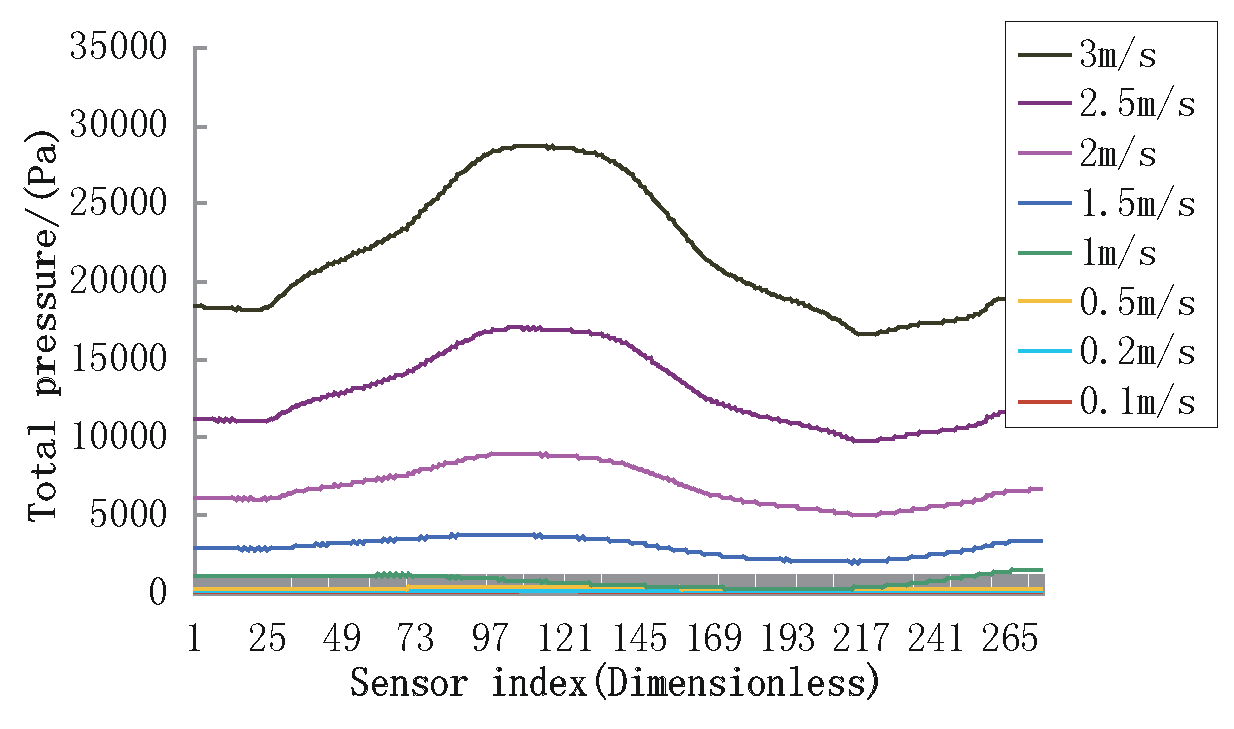
\includegraphics[width=11cm]{figure/chap3/fig6a_pressure_0.pdf}
        \label{fig:chap3:F13}
        \bicaption[fig:chap3:F13]{来流角为0度时的总压强对比}{来流角为0度时的总压强对比} {Fig.}{Comparison of total pressure with inflow angle is zero degree}
    \end{figure}
%    \hspace{0.5in}
%    \vspace{0.5in}
    \begin{figure}[!htp]
        \centering
        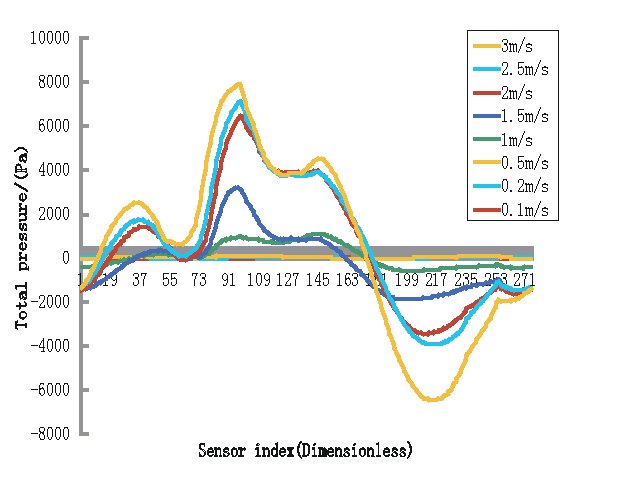
\includegraphics[width=11cm]{figure/chap3/fig6b_pressure_60.pdf}
        \label{fig:chap3:F14}
        \bicaption[fig:chap3:F14]{来流角为60度时的总压强对比}{来流角为60度时的总压强对比} {Fig.}{Comparison of total pressure with inflow angle is 60 degree}
        %\label{fig:pre60}
    \end{figure}

    \begin{figure}[!htp]
        \centering
        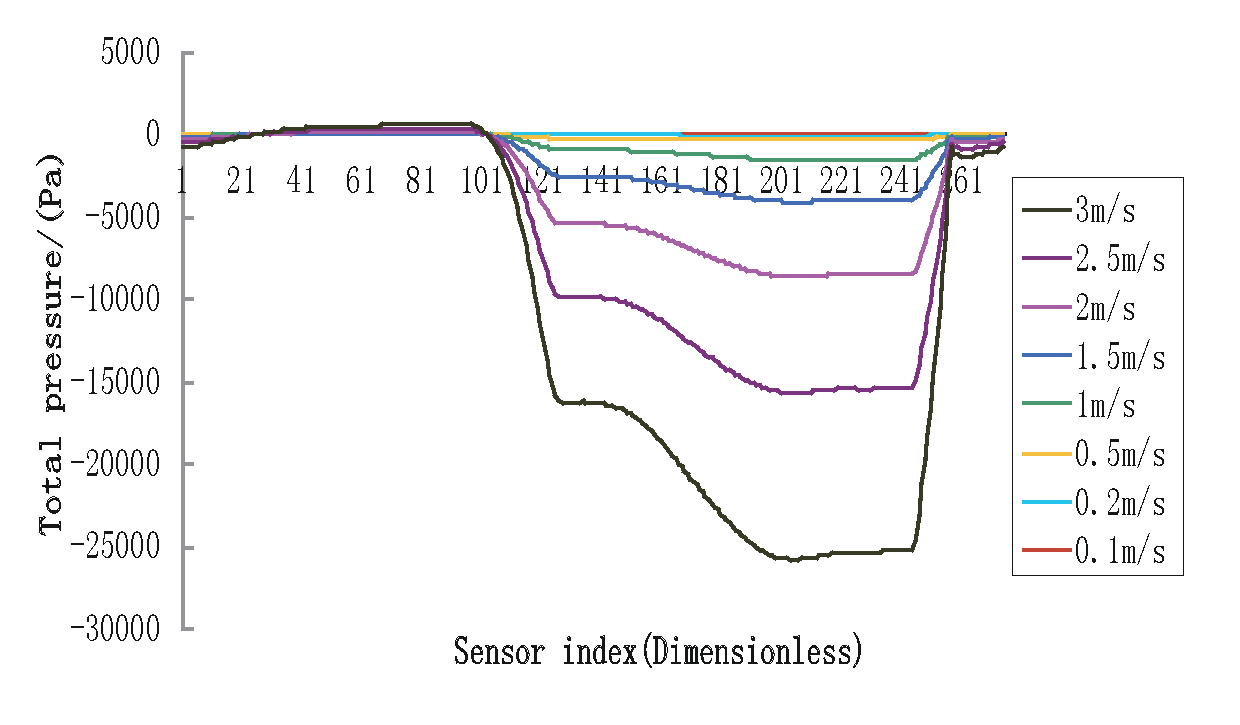
\includegraphics[width=11cm]{figure/chap3/fig6c_pressure_90.pdf}
        \label{fig:chap3:F15}
        \bicaption[fig:chap3:F15]{来流角为90度时的总压强对比}{来流角为90度时的总压强对比} {Fig.}{Comparison of total pressure with inflow angle is 90 degree}
        %\label{fig:pre90}
    \end{figure}
    % \bicaption[fig:fig6abc]{图}{不同来流的总压力比较:每个图中的图例表示流速的大小.} {Fig}{Comparison of total pressure of different flow: legends in each figure represent the magnitude of flow velocity. }


A. {测试运动评价权重}

本部分提出的三个权重标准被提出是用来评估航行器周围的瞬态冲击和能量分布情况。$W$ 是流速测试的一般权重,$Wv$ 是考虑流体冲击效应的速度评估权重,$Wvv$ 是用来反映能量分布情况的速度平方权重。三个权重的对比可以参考图\ref{fig:chap3:F16}。

\begin{figure}[!htp]
    \centering
        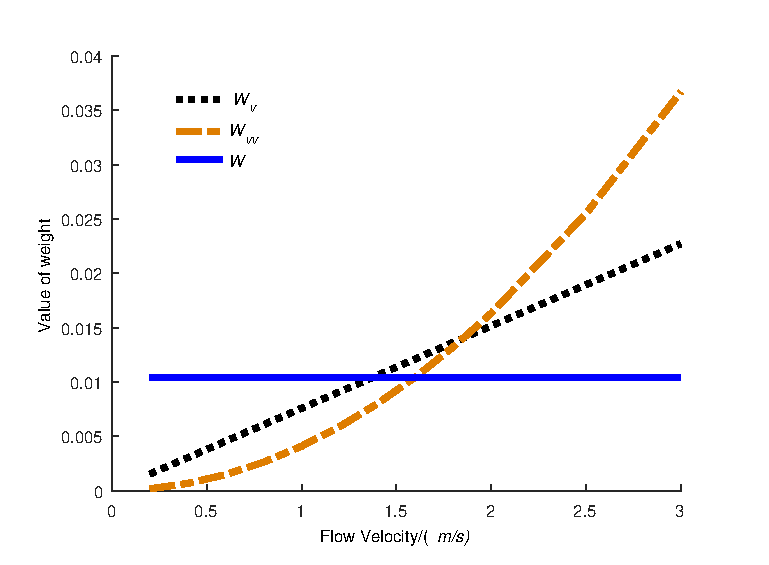
\includegraphics[width=10cm]{figure/chap3/fig7_weigiht_EnglishVersion.eps}
        \label{fig:chap3:F16}
        \bicaption[fig:chap3:F16]{不同的评价权重对比图}{不同的评价权重对比图} {Fig.}{Comparison of different weights}
\end{figure}

B. {选取最优支持向量机内核函数}

水流预测主要分为识别流向和估计流速大小,和人类感知风的情况相似,因此水流分类的工作侧重于流向的识别。 由于支持向量机有各种类型的内核函数,因此,使用不同的分类器测试了水流流向的辨识效果,并可以从表\ref{table:chap3:kenerls}中的测试结果选择出最佳的内核函数。

\begin{table}[!htp]
  \centering
  \label{table:chap3:kenerls}%
  \bicaption[table:chap3:kenerls]{不同内核的测试结果对比}{不同内核的测试结果对比} {Table}{Testing results for each kernel }
    \begin{tabular}{cccc}
    \toprule
    kernel type & $W$ & $W_v$    & $W_{vv}$ \\
    \midrule
    linear & 0.7708 & 0.9091 & 0.9436 \\
    Quadratic & 0.8438 & 0.9045 & 0.8847 \\
    Polynomial & 0.9271 & 0.9545 & 0.9462 \\
    RBF   & 0.7396 & 0.8333 & 0.8366 \\
    multilayer perception & 0.2185 & 0.247 & 0.2549 \\
    \bottomrule
    \end{tabular}%
\end{table}%

C. {特性提取 }

压力数据是从流体分析模型的航行器的体表上提出的,由于节点较多,提出的压力数据维度较高,因此为了便于后续处理,需要对数据进行预处理。基于压缩感知的思想,将数据压缩且不失去数据中的大部分信息是可行的。这里使用了线性判别分析对压力数据进行处理,预先标记一些数据,将数据投影到更低的维度,形成新的可以反映数据特征的特征向量。需要指出,特征向量的个数是由标记的数据的类的个数来定,这里的最大特征向量个数为7个。将获得的特征向量输入到分类器里面,并进行不同运动效应下的分类效果对比,如表\ref{table:chap3:sevenvector}。

% Table generated by Excel2LaTeX from sheet 'Sheet1'
\begin{table}[!htp]
  \centering
  \label{table:chap3:sevenvector}%
  \bicaption[table:chap3:sevenvector]{七特征向量的分类效果}{七特征向量的分类效果} {Fig.}{LDA compressed SVM classification for seven feature vectors }
    \begin{tabular*}{7cm}{cccc}
    \toprule
    Weight type & \textit{W} & \textit{Wv} & \textit{Wvv} \\
    \midrule
    Correct rate & 0.9375 & 0.9697 & 0.9625 \\
    \bottomrule
    \end{tabular*}%
\end{table}%

AUV 运行的水下环境是实时多变的,为了更及时获取水流的方向模式,文中对所有的2个特征矢量组合选择进行测试,测试效果见图\ref{fig:chap3:F17},不同的特征矢量组合获得的测试效果呈现不同的差异,不同的评价权重也会得到不同的特征矢量选择。

\begin{figure}[!htp]
    \centering
        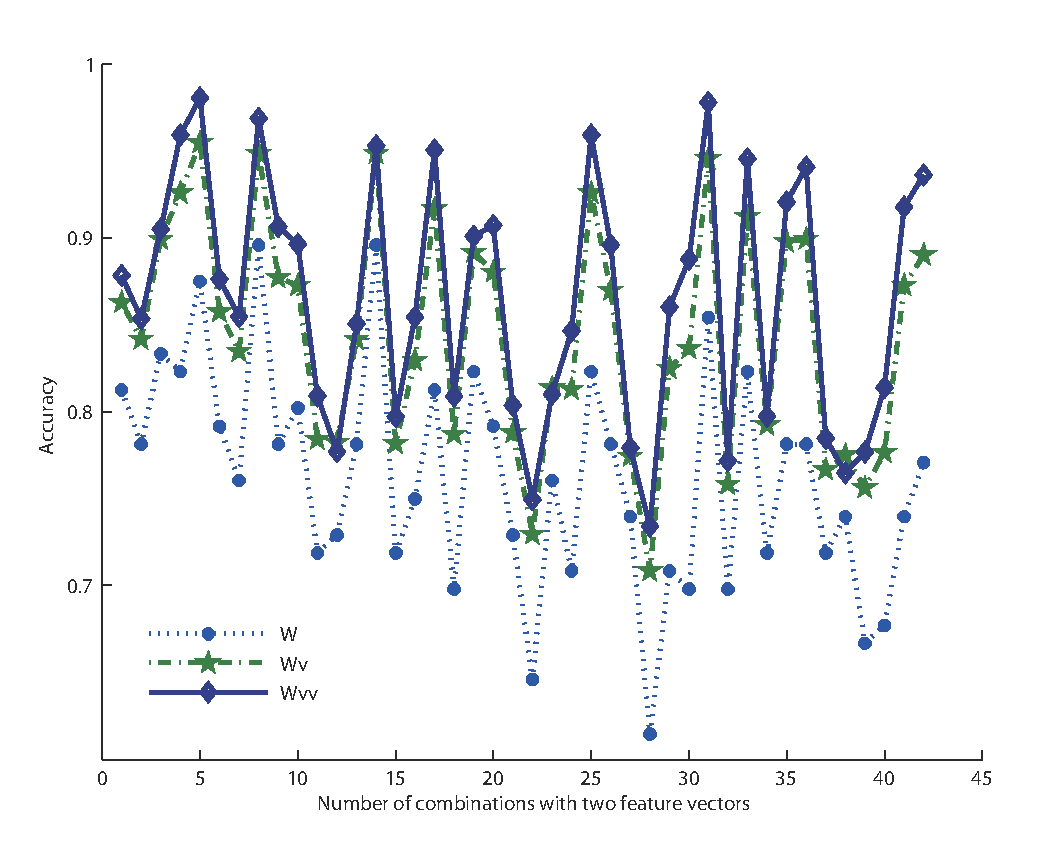
\includegraphics[width=14cm]{figure/chap3/fig8_Total_LDA_two_eigvalue_accurry_EnglishVersion1.pdf}
        \label{fig:chap3:F17}
        \bicaption[fig:chap3:F17]{两特征向量的组合分配测试效果}{两特征向量的组合分配测试效果} {Fig.}{Two feature vectors combined evaluation }
\end{figure}

D. {速度大小估计 }

不同的水流方向上水流速度的大小也是不同,由于不同水流的速度的作用,AUV 本体上受到的压力也是不同,图\ref{fig:chap3:F18} 为不同水流方向下不同流速的压力最大值最小值。为了在判定水流大小后,进而确定出水流的速率,文中使用速度与对应压力极值分别拟合各方向的水流值。拟合的测试270º 流向速度压力极值方程见图\ref{fig:chap3:F19}。

\begin{figure}[!htp]
    \centering
        %\noindent\makebox[\paperwidth][c]
        {
        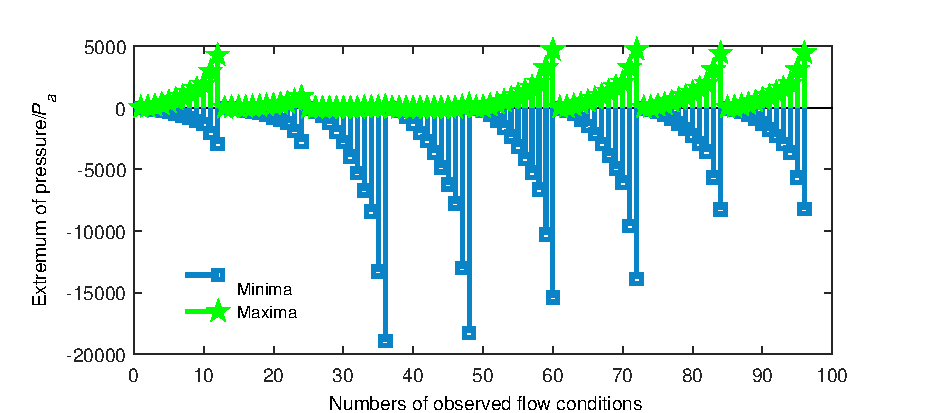
\includegraphics[width=14cm]{figure/chap3/fig9_press_value_maxmin_EnglishVersion1.eps}
        }
        \label{fig:chap3:F18}
        \bicaption[fig:chap3:F18]{压力数据极值}{压力数据极值} {Fig.}{Pressure extremes }
\end{figure}

\begin{figure}[!htp]
\centering
\subfigure[Maxima pressure $P_{max}/P_a$]{
\label{fig:chap3:F19a}
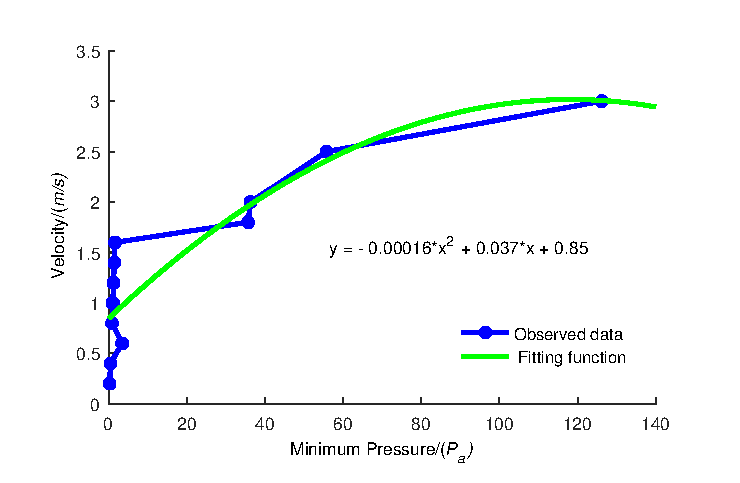
\includegraphics[width=10cm]{figure/chap3/fig10a_maximum.eps} }
\hspace{1in}
\subfigure[Minimum pressure $P_{max}/P_a$]{
\label{fig:chap3:F19b}
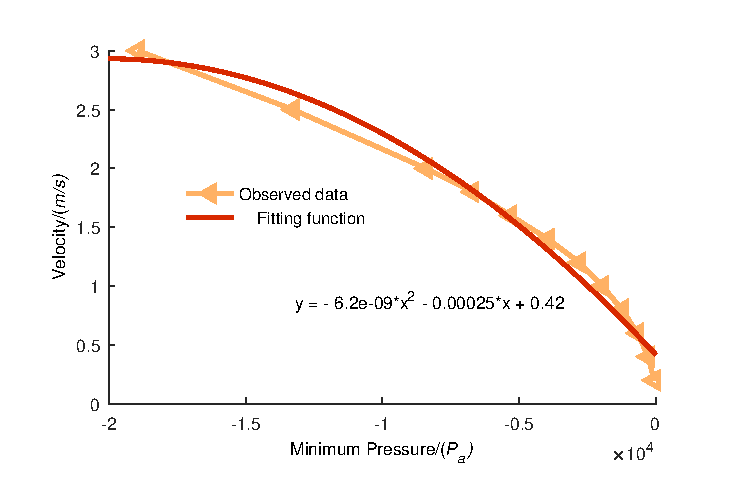
\includegraphics[width=10cm]{figure/chap3/fig10b_minimum.eps} }
\label{fig:chap3:F19}
\bicaption[fig:chap3:F19]{270度来流的流速预测方程}{270度来流的流速预测方程} {Fig.}{Fitting pressure equation of flow rate in 270-degree flow }
\end{figure}



\begin{table}[!htbp]
% %\tiny
%   %\onecolumn
  \centering
  \label{table:chap3:verification}
  \bicaption[table:chap3:verification]{水流预测结果}{水流预测结果}{Table}{Results comparison of flow forecasting }
  \begin{tabular}{ccccccc}
  \toprule
  \multirow{2}{*}{Flow direction estimation} & \multicolumn{4}{c}{Flow angle / $\left (degree\right )$} \\
                           &135    &270    &0      & 45    &90    &180 \\
  \midrule
  Actual flow rate/($m/s$) &1.8    &1.6    &1.8    &1      &1.6    &2.5 \\
      \\
  Test flow rate /($m/s$)  & 1.818 &1.2566 &1.1817 &0.888  &1.3226 &2.63 \\
  \bottomrule
  \end{tabular}%
\end{table}%

E. {分类器测试 }

为验证建立的水流方向模式识别模型与流速估计方法的有效性,以随意选取的且未被使用过的多个水流压力数据进行预测,获得如下测试效果(表\ref{table:chap3:verification})。

由表\ref{table:chap3:verification}可以验证,LDA-SVM 分类器能够有效地判断水流流向,并在一定范围内有效地计算出水流速度,这与生物感知空气场与流体场的结果相同。

F. {水下机器人运动学与水流预测模型的关系探讨   }

\begin{algorithm}[!htbp]
\centering
\caption{侧线估计偏航角的流程 \protect \\\quad \quad Framework of how to measure yaw angle based on lateral line}
\label{Algorithm:chap3:Framwork}
% \bicaption[Algorithm:chap3:Framwork]{侧向估计偏航角的框架流程}{侧向估计偏航角的框架流程}{Fig.}{Framework of how to measure yaw angle based on lateral line}
\begin{algorithmic}[1]
\REQUIRE
The pressure sensor node value around vehicle body is $P \left (t,i \right )$ at time $t$. The initial orientation angle of yaw motion, set $\psi_{t=0} =0$, and assuming the water environment is stable, so $V_{flow_{t}}$ is constant, and $R\left (\varphi,\theta,\psi  \right )\approx R\left ( \psi \right )$ in surface plane motion;\\

%The set of positive samples for current batch, $P_n$;
%The set of unlabelled samples for current batch, $U_n$;
%Ensemble of classifiers on former batches, $E_{n-1}$;
\ENSURE
The yaw angle of vehicle, $\psi_t$;
%Ensemble of classifiers on the current batch, $E_n$;
\FORALL{$t= j$ in $T$}
    \STATE forecast the velocity direction of flow: \\
    $ v_{direction} = f_{LDA-SVM}\left ( P \left (t,i \right ) \right )$;
    \STATE calculate the magnitude of flow velocity: \\
    $v_{magnitude} = w_1\ast g\left(min\left( P \left (t,i \right ) \right)\right)
    + w_2 \ast  h\left(max\left(    P \left (t,i \right )    \right)\right)   $, \\where $w_k =0.5$  is the component weight, $k = 1,2$;\\

    \STATE ${v_{flow_t}}$ is composed with $ v_{direction}$ and $v_{magnitude}$;
    \IF{$t=1$}
        \STATE $ \psi = 0 $
        \STATE $ V_{t-1} = V_t $,
        that is $V_{t=0} = v_{flow_{t=0}}$;
    \ENDIF

    \STATE ${V_{flow_t}}= R\left( \psi_t \right){v_{flow_t}}
    = R\left( \psi_{t=0} \right){v_{flow_{t=0}}}$;\\
    \STATE yaw angle $\psi_t$ is known from $v_{flow_{t=0}}$ and $v_{flow_t}$;
\ENDFOR
\RETURN
 $\psi_t$;
\end{algorithmic}
\end{algorithm}


在水下机器人的体坐标系内,水流的模型被进行了分类判定。这个分类模型可以用在两种情况下:一种是静水中,航行器航行时的水流感知,一种是航行器静止,有水流情况的识别。水流是可以在惯性坐标系下进行表示的,从方程\ref{eq:chap3:30}中可获得的水平面内的水流流向角度 $\psi$,方程表示如下:

\begin{equation}
\label{eq:chap3:30}
V_t = R\left (  \varphi,\theta,\psi \right )v_t
\end{equation}
其中, $R\left ( \varphi,\theta,\psi \right )$ 是体坐标系和惯性坐标系之间的变换矩阵,$v_t$ 是在时间$t$的体坐标系中使用LDA-SVM分类器预测的流速(包括方向和速率大小)。当机器人在水中导航时,环境是稳定的,就可以同时识别出水流。 当 $t=0$ 时,机器人第一次感知当前状态,$v_{t=0}$ 是已知的,因此,考虑到水下环境是稳定的假设,可以得到 $V_{t=0}$。 因此,机器人的姿态角可从算法\ref{Algorithm:chap3:Framwork}中计算出来。 然而,由于来流相对于航行器本体是会变化的,航行器的运动将导致不同的姿态角估计,主要是航向角 $\psi$。预测水流是在给定的表面平面运动条件下的,水流是不变的。基于这个参考量就可以通过坐标系转换运算来计算航行器在体坐标系中的速度,这点和水里生活的盲鱼感知方向在本质上是统一的。不足的是,本章提出的水流辨识方法基于流体仿真中获取的数据,因此水流中的噪声源影响性评估以及深度变化带来的影响需要进行系统的实验研究。


\section{本章小结 }

本章系统地研究了水下机器人REMUS AUV的模型搜索与辨识问题,并从利于水下机器人认识水下环境的角度,基于鱼类体线感知水流的生物机理,采用机器学习方法研究水下机器人周布压力传感器阵列识别水流模式的热点问题。为便于对系统建模中的参数辨识类方法与符号回归方法的不同进行研究,建立时间序列数据集构成的目标函数,并说明了符号功能矩阵与模型结构以及系统建模的关系。在本章中,分别将阻尼系数的真实值作为对比,然后使用Levenberg-Marquardt方法、遗传算法、基于遗传编程技术的符号回归算法对模型参数进行估计。并且为了确认噪声影响,建立了传感器SNR模型,以确定不同噪声下的辨识效果的差异。为了搜索模型的新结构,还将符号回归方法用来搜索模型的最近似结构,以便于自适应控制应用。本章中,为辨识水流环境,提出一种基于LDA和SVM结合分类器来辨识水流方向。通过使用压力传感器阵列获取反映水下机器人周围模型水流变化的压力数据,并使用LDA方法压缩压力感知以获取最优的特征向量矩阵。使用最优的SVM内核函数对水流的流向进行了预测,并使用拟合方法估计流速。实验结果表明了本章提出的系统模型搜索方法和水流环境识别方法的可行性,对水下机器人模型确定与海洋认知有一定参考性。

%# -*- coding:utf-8 -*-
%!TEX root = ../thesis.tex



\chapter{控制导向的水下机器人模型建立}
% P86-P115
\label{chap:modelingforcontrol}
% 4.1 引言
% 4.2 控制导向的数学模型
% 4.3 鱼雷型机器人的模型建立
% 4.4 复杂外形机器人的模型建立
% 4.5 计算结果与分析
% 4.6 本章小结
\section{引言 }
水下机器人的模型用来解释本体运动与施加在本体上的力、力矩之间的关系,该模型对于控制和导航都具有重要作用。水下机器人系统需要进行水下航行来验证系统的可行性。然而,用于描述水下机器人动力学特征的数学模型并非完全适用于水下机器人的控制系统设计。动力学、运动学理论常常被用来分析水下机器人的运动,这种方法可以帮助研究者从数学原理的角度对运载器的本体的系统行为有个理性认识。非线性模型识别是基于实验数据对水下机器人系统进行动力学模型参数的估计。研究人员会基于固有的知识,如已经建立的模型,或者使用室内水池实验提取的测试数据,进行水下机器人的搜索和系统辨识。然而,数学描述法和系统辨识方法建立的模型主要是为了研究系统行为,而水池实验所需要的成本较高,需要对水下机器人模型有个深度的了解。这些特点都对于水下机器人的控制器设计带来挑战。

合适的控制器对水下机器人成功地进行水下航行与执行任务非常关键。控制器主要分为无模型控制和有模型控制。无模型控制方法能力强大,但是应用该方法训练水下机器人在未知环境中航行需要花费较多的时间进行调节参数,以及无法保证控制器的鲁棒性和自适应性。鲁棒自适应控制方法可以应对水下机器人在适应未知环境中工作时参数变化,稳定地应对一定形式的干扰。因此需要进行用于控制导向的水下机器人模型构建方法研究。

用于鲁棒控制的水下机器人模型建立方法受到了研究者的关注。Yang和Clement等对于小型AUV的运动特点进行研究,分析了水下机器人动力学模型中各项的重要性,并使用数值分析方法为鲁棒补偿器控制建立的水下机器人模型\cite{yang2015modeling}。该方法是基于水下机器人的CAD模型进行数值分析的,并与实验进行对比。虽然数值分析方法可以提供精确度较高的模型,但是其计算量大,且对控制器设计带来一定的流体分析挑战。基于经验数据而对水下机器人模型进行估算也是一个有效且快速的方法,该方法仅仅需要ROV的有关尺寸参数就可以进行ROV模型构建,其中刚度模型质量矩阵也可以采用CAD软件进行测量获得。相比于数值分析法,该方法计算快速,便于编译成一个计算程序,这对于水下机器人的控制器设计很有益。数值分析法和经验法都是可以基于水下机器人的外形进行建模,建立的模型可以适用于非初等几何形状的运载器控制,结合自适应估计部分则可以加强机器人的水下自适应性。具有非初等几何形状的机器人主要是ROV,而与之相比,AUV有很好的流线型,AUV的模型可以参考潜艇模型或者使用系统辨识方法获得模型,但是AUV的数学模型需要进行数学简化方可适用于水下机器人。一般而言,非线性模型的简化是粗略地忽略一些变量,这种方法忽视了各种量的相关性,会给系统控制带来干扰。本部分介绍了一种基于泰勒公式展开的方法,可以将复杂的非线性模型简化为适用于自适应控制的简化模型。


\section{非初等几何外形的水下机器人模型建立}

水下机器人根据流体力学的分布情况,分为流线型的和非流线型的水下机器人。流线型水下机器人的建模多参考潜艇模型简化建立用于控制的模型。非流线型的水下机器人因形状复杂而具有较多的非初等集合外形。在本节中,将介绍具有初等几何外形的水下机器人的建模方法:一种是经验法,另外一种是流体力学软件计算法\cite{eidsvik2015identification,elgenes2017underwater}。两种方法都可以用来计算ROV的模型,并将模型用于控制器设计。

\subsection{经验法}

本节中,将介绍一种估算水下机器人ROV的典型流体动力学参数的方法。估算ROV的流体动力学的参数,应包括质量项,阻尼项,恢复力项。该方法可以用于对多种形状的ROV机器人进行建模,包括作业型ROV和观测型ROV。估计法是基于经验并对实验数据进行分析而总结的一个方法,该方法可以用于不同形状的ROV模型分析\cite{bertram2012practical}。当要采用这种方法对水下机器人进行模型快速估算时,可以保证有相当高的精度。此外,该方法也不需要对ROV模型有很深的了解。在本部分的进一步工作中,由于刚体质量矩阵的系数可以非常容易地从CAD绘图或估计中获得,在本节中进行的这些参数的介绍较少。本节的研究重点将是更难以获得的附加质量和阻尼系数。

\subsubsection{质量项}
质量矩阵中的项是很简单的几何量。如果水下机器人的CAD模型存在,就很容易获得这些项的数值。如果一个CAD模型并不存在,那个这些系数则需要采用积分和平行轴线理论来求取。在进行估计是,假设ROV质量为$m$ [kg]。

在计算与平动有关项时,假设质量是在ROV整个体积内平均分布的。因为ROV在空气中的重量是已知的,因此平动项也可以获得,即,$M_{11} = m$  [kg], $M_{22} = m$ [kg], $M_{33}=m$ [kg]。

旋转自由度系数被定义为力矩和惯性的乘积。对角线上的项称为惯性力矩,其可以由如下公式计算:

\begin{equation}
I_p =  \int_{V}\rho \left ( r \right )\ast r^{2}dV = m \ast r^{2}
\label{eq:chap4:mass}
\end{equation}

假设ROV是矩形体,这样可以得到水下机器人ROV的各个轴的惯性转矩如下:

\begin{equation}
\begin{aligned}
I_4 &= \frac{m}{12}\left ( W^2 + H^2 \right ) \\
    &= \frac{m[kg]}{12}\left ( (W[m])^2 + (H[m])^2) \right )\\
    &= I_4[kgm^{2}] \\
I_5 &= \frac{m}{12}\left ( L^2 + H^2 \right ) \\
    &= \frac{m[kg]}{12}\left ( (L[m])^2 + (H[m])^2) \right )\\
    &= I_5[kgm^{2}]\\
I_6 &= \frac{m}{12}\left ( W^2 + L^2 \right ) \\
    &= \frac{m[kg]}{12}\left ( (W[m])^2 + (L[m])^2) \right )\\
    &= I_6[kgm^{2}]
\end{aligned}
\label{eq:chap4:massrot}
\end{equation}

因假设水下机器人是纯矩形的,那么水下机器人的重心就和几何重心重合,那么其他的不在对角线上的耦合惯性转矩是为零的。

\subsubsection{恢复力}

对于水下机器人而言,当水下机器人本体完全没入到水中时,浮力常常是略大于重力的。这样设计是为了确保,当水下机器人在运行时出现能源中断(耗尽)以及别的系统故障时,水下机器人能够重新浮出水面,而不至于丢失。然而,这个净浮力相比于水下机器人的本体重力往往是比较小,因此在本文进行力平衡分析时候,可以忽略。图\ref{fig:chap4:F1} 是俯仰自由度的恢复力的物理原理图\cite{eidsvik2015identification}。 同理,也可以进行横滚自由度的恢复力分析。

\begin{figure}
\label{fig:chap4:F1}
\centering
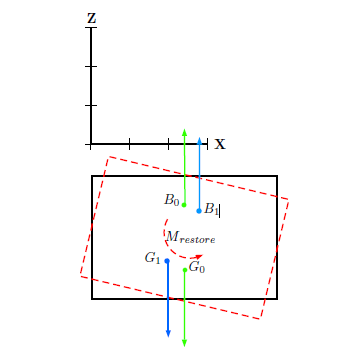
\includegraphics[width = 6cm]{figure/chap4/restoring.png}
\bicaption[fig:chap4:F1]{恢复力原理示意图}{恢复力原理示意图}{Fig.}{Restoring moment concept}
\end{figure}

使用三角法,很容易找到横滚自由度和俯仰自由度的恢复力矩。因为本体上的重心和浮心之间距离是固定的,所以恢复力矩只与浮力和重力之间的力臂长度有关。

如前面所述,ROV在设计的时候往往会让浮力略大于重力,使之具有正浮性。在进行恢复力分析时,是假设重力是等于浮力的,因此重力矢量和浮力矢量之间的力臂长度才是最重要的参数。要估计恢复力矩的大小,就要确定出力臂的长度,但是一般而言,力臂长度很难被估计出来。使用一些CAD软件例如CATIA、 HydroD可以帮助研究者快速的确定重心和浮心的位置。而使用经验法进行估计水动力学参数时,假设浮心的位置是已知的。如此,可以获得ROV的横滚自由度和俯仰自由度的恢复力的公式如下:

\begin{equation}
\begin{aligned}
C_{44} &= -(z_g \ast W-z_b \ast B)\ast cos(\theta) sin(\varphi) \approx W \ast \overline{BG} \ast 1 \ast \varphi \\
C_{55} &= -(z_g \ast W - z_b \ast B) \ast cos(\varphi) sin(\theta) \approx W \ast \overline{BG} \ast 1 \ast \theta\\
B &= W = m \ast G = 9.81 \ast m [N]\\
\label{eq:chap4:restor}
\end{aligned}
\end{equation}
其中,$\overline{BG}$ 是重心和浮心之间的垂直距离。

如果$z_{g}$为零,并且ROV的俯仰与横滚满足小角度理论,那么可以将公式重写如下:

\begin{equation}
\begin{aligned}
C_{44} &\approx (9.81 \ast m) \ast \overline{OB}  \ast \varphi [Nm]\\
C_{55} &\approx (9.81 \ast m) \ast \overline{OB}  \ast \theta [Nm]\\
\end{aligned}
\end{equation}
其中,$\overline{OB}$ 是旋转中心到浮力的距离。

\subsubsection{附加质量}

为了估算ROV的附加质量,就需要使用分析数据。有很多的数据源可以使用,但是在使用这些数据源时候必须采用DNV标准\cite{DNVStard}。DNV标准中采用矩形体的其中两个面作为参考。该假设对于本论文中的ROV是可以适用的,因为所有的ROV都有近似的高度和宽度。高度和宽度的平均值将可以被用来求解估计数据。

因为参考值中假设ROV是矩形体,但是ROV并不是完全的实体,ROV中会有空隙,也会存在渗透流。这个影响可以通过使用一个缩放系数$C_{p}^{mn}$ 对参考值进行校正。该系数是用上标平面内的投影面积除以参考矩形体的平行面的面积而求取。在表\ref{tab:chap4:table1}中列出了用于获得相关投影面积系数的局部坐标系\cite{bertram2012practical}。

\begin{table}
\centering
\label{tab:chap4:table1}
\bicaption[tab:chap4:table1]{投影面积所对应的系数上标}{投影面积所对应的系数上标}{Table}{Projected area coefficient superscript}
\begin{tabular}{cccc}
\toprule
 DOF            & m & n & o\\
\midrule
 Surge \& roll  & X  &Y   &Z   \\
 Sway  \& pitch &  Y &Z   &X   \\
 Heave \& yaw   &Z   &X   &Y   \\
\bottomrule
\end{tabular}
\end{table}

根据DNV标准\cite{DNVStard},矩形体的附加质量的数据如表\ref{tab:chap4:table2}所示。

\begin{table}
\centering
\label{tab:chap4:table2}
\bicaption[tab:chap4:table2]{附加质量系数}{附加质量系数}{Table}{Added mass coefficients}
\begin{tabular}{cccc}
\toprule
 Body shape  & Dimensions(B/A) & Added mass coefficient\\
\midrule
\multirow{7}{4cm}{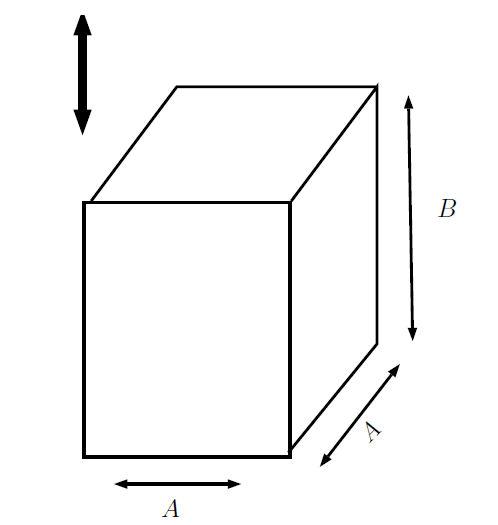
\includegraphics[width = 4cm]{figure/chap4/T2_f.png}}
 & 1.0   &0.68    \\
 & 2.0   &0.36    \\
 & 3.0   &0.24    \\
 & 4.0   &0.19    \\
 & 5.0   &0.15    \\
 & 6.0   &0.13    \\
 & 7.0   &0.08    \\
\bottomrule
\end{tabular}
\end{table}


对于旋转自由度,没有找到经验3D数据。 不同的
因此必须使用方法。 使用类似形状的知识之一
知道球体(3D)的附加质量差异和无限长的差异
相同半径(2D)的圆柱体为50%\cite{bertram2012practical}。 通过将这个关系转换成问题
手头可以创建一个旋转自由度的程序。

对于水下机器人的旋转自由度,并没有找到3D经验数据。因此必须采用不同的方法来进行分析。可以通过找不同形状的附加质量之间的相似性,来研究附加质量之间的关系,例如,相同直径的三维球体和无限长的二维圆柱体的附加质量相差50$\%$。通过将这种关系转成手头可以处理的问题,就有可能创造出一个旋转自由度的附加质量求解程序。

求解程序如下:
步骤一:使用经验3D数据找到平动自由度的附加质量;
步骤二:使用2D数据和切片理论确定平动自由度的附加质量;
步骤三:使用缩放系数对比两种方法的不同;
步骤四:使用2D数据和切片理论找到旋转自由度的附加质量;
步骤五:对结果进行调整。

通过使用以上流程,就有可能找到附加质量矩阵对角线上的所有项。

为了利用好参考的经验数据, 一个合适的缩放程序就需要考虑ROV和参考的矩形体之间的差异。有很多种方法可以用来处理这个差异,但是在众多的方法中能够对所有的量都能做到获取便捷才是最佳的选择。在本文中,附加值质量系数是使用投影面积进行缩放调整的。投影面积可以使用CAD软件如CATIA获取,分别测量出三个平面的投影面积。此外,也可以手动地测量估算出来ROV在三个平面的投影面积。这个投影面积然后被用来计算系数$C_{p}^{mn}$。因此,可以得到三个平面的系数计算公式如下:

\begin{equation}
\begin{aligned}
C_{p}^{XY} = \frac{A_{p}^{XY}}{A} = \frac{A_{p}^{XY}}{L \ast W} \\
C_{p}^{YZ} = \frac{A_{p}^{YZ}}{A} = \frac{A_{p}^{YZ}}{H \ast W} \\
C_{p}^{ZX} = \frac{A_{p}^{ZX}}{A} = \frac{A_{p}^{ZX}}{L \ast H} \\
\end{aligned}
\end{equation}

对于平移运动的附加质量,往往首先是对纵荡运动进行分析。通过观察表,可以发现$\frac{B}{A}$的最小值为1.0。这也就意味着只有水下机器人的长度尺寸大于宽度和高度尺寸时候,参考的数据才是有效的。这个要求对于大多数的水下机器人都是成立的。

第一步是为$A_{11}$找到相应的经验3D系数。 查询表格值需要确定出ROV的高度与宽度。 因为表格仅包含给定数量的数据点
($\frac{b}{a}$)值,对于数据集在这两数据点之间的情况就需要进行线性化差值。

数据点之间的距离线性化是采用如下公式来计算经验值:

\begin{equation}
\begin{aligned}
C_a(\frac{b}{a}) = \frac{C_a(2)-C_a(1)}{X_2 - X_1} \ast  (X - X_2) + C_a(2)
\end{aligned}
\end{equation}

然后,需要计算参考体积:

\begin{equation}
\begin{aligned}
V_R = b \ast a^2
\end{aligned}
\end{equation}

修正后的附加质量公式如下:

\begin{equation}
\begin{aligned}
A_{ij} = C_a V_R \rho_{water}(C_p^{no})^2(C_p^{mo})^(C_p^{mn})
\end{aligned}
\end{equation}

这样,$A_{11}$ 就可以使用3D数据进行计算并给出一个相对合理的估计。

同样地,其余的附加质量系数也可以采用切片理论并参考2D的系数和DNV标准进行估算。第一步就是确定宽度与高度的关系。然后,将宽高比的数值带入到方程中来获得附加质量系数。当使用切片理论时,需要计算参考面积而不是参考体积:

\begin{equation}
\begin{aligned}
A_R = \pi \ast (a)^{2}
\end{aligned}
\end{equation}

这样,就可以得到纵荡自由度的2D附加质量系数:
\begin{equation}
\begin{aligned}
A_{11}^{2D} = \rho \ast C_a A_r(C_p^{no})^2(C_p^{mo})(C_p^mn)
\end{aligned}
\end{equation}

通过应用切片理论,对2D的附加质量进行积分,可以获得3D附加质量如下:

\begin{equation}
\begin{aligned}
A_{11} = \int_{L/2}^{-L/2}A_{11}^{2D}dx
\end{aligned}
\end{equation}

这样就可以找到切片理论和3D计算之间差异:

\begin{equation}
\begin{aligned}
\lambda = \frac{A_{11}^{empirical-3D}}{A_{11}^{strip-3D}}
\end{aligned}
\end{equation}
缩放系数$\lambda$ 给出了两个方法之间的关系。因此显而易见的是,如果这种关系对于所有自由度都是有效的,则可以使用切片理论计算附加质量,然后缩放以获得正确的附加质量估计值。

对于旋转自由度,也可以采用和平移自由度内类似的方法,使用缩放系数对切片理论计算的结果进行调整。2D的附加质量系数可以从DNV的有关标准中查阅。旋转自由度的2D附加质量的一般公式为
\begin{equation}
\begin{aligned}
A_{ii}^{2D} = \rho \ast C_a \ast \pi a^4 (C_p^{no})(C_p^{mo})(C_p^{mn})
\end{aligned}
\end{equation}

在整个长度上进行积分,可以得到

\begin{equation}
\begin{aligned}
A_{ii}^{'} = \int_{(L,B,H)/2}^{-(L,B,H)/2}A_{ii}^{2D}dx
\end{aligned}
\end{equation}

最近进行缩放调整,就可以得到旋转自由度的附加质量系数:

\begin{equation}
\begin{aligned}
A_{ii} = A_{ii}^{'} \lambda [kgm^{2}]
\end{aligned}
\end{equation}

\subsubsection{阻尼力}

ROV的阻尼力是和机器人的运行速度有关的。如果阻尼是高度非线性的,就很难对其进行准确地估计。

为了分析水下机器人的阻尼,就必须对阻尼的概念有所介绍。第二章在水下机器人的模型部分介绍了一些相关知识。ROV受到阻尼主要包括线性和二次摩擦阻尼以及由于旋涡脱落而产生的相关阻尼。由于旋涡脱落而产生的阻尼可以建模为二阶方程(莫里斯方程)。这样ROV受到的阻尼主要可以使用线性和二阶阻尼的合系数来描述其作用大小。

\begin{equation}
\begin{aligned}
B = B ^{LIN} + B ^{NL}
\end{aligned}
\end{equation}
其中,$B ^{LIN}$是线性阻尼系数,$B ^{NL}$是非线性阻尼系数。

线性阻尼部分包括线性摩擦阻尼;而非线性阻尼则包括了所有的高阶阻尼项,例如湍流摩擦阻尼和旋涡脱落而产生的阻尼。对于低速航行的ROV,由于湍流和漩涡而产生的阻尼作用小,线性阻尼会是主要的部分。同样,高速航行的水下机器人中,非线性阻尼会起主要的作用。因此,显而易见的是,两种阻尼对于描述ROV在整个运行阶段中的阻尼行为都是至关重要的。

如前所述,二次阻尼表示所有高阶阻尼的贡献,但主要是涡旋脱落和湍流边界层表皮摩擦。 可能从线性阻尼开始更符合逻辑,但是对于经验性的角度来说,利用Morison方程估计二次阻尼更容易。 使用势能理论并不能求得二次阻尼,因为势能理论假定水是无旋转的,不可压缩的和无粘性的流体。 这种假设对于许多应用来说是足够的,但是当涉及阻尼时,就必须考虑水的粘度的作用。

正如附加质量一样,唯一可用的3D参数是纵荡自由度的3D阻力系数,并且这里仍然假定ROV的长度大于宽度和高度。因此,估计步骤类似于附加质量。二次阻尼将使用3D系数估算,然后使用Morison方程进行估算。 将估算的结果进行缩放,然后再将相同的缩放数量应用于剩余自由度里。如前所述,阻力系数是纯粹用于描述特定几何形状的粘滞阻力的经验系数。由于ROV的尺寸已知,因此可以通过查询相关文献找到3D和2D阻力系数\cite{eidsvik2015identification,bertram2012practical}。

应当指出阻尼系数的公式如下:

\begin{equation}
\begin{aligned}
C_D = \frac{F_D}{\frac{1}{2}\rho \ast A \ast u \left | u \right |}
\end{aligned}
\end{equation}

平移运动的二次阻尼系数可以使用莫里斯方程得到,公式如下:

\begin{equation}
\begin{aligned}
B_{jj}^{NL}v_j|v_j| = \frac{\rho}{2}C_D A v_j |v_j| \lambda(C_p^{no}), j = 1,2,3
\end{aligned}
\end{equation}

需要注意的是莫里斯方程里的参考面积是使用投影面积进行缩放调整得到。2D的切片理论和3D的阻尼系数的差异需要被计算出来。对莫里斯方程的所有必要的术语进行修正,就可以计算出平移自由度阻尼。

\begin{figure}
\label{fig:chap4:F2}
\centering
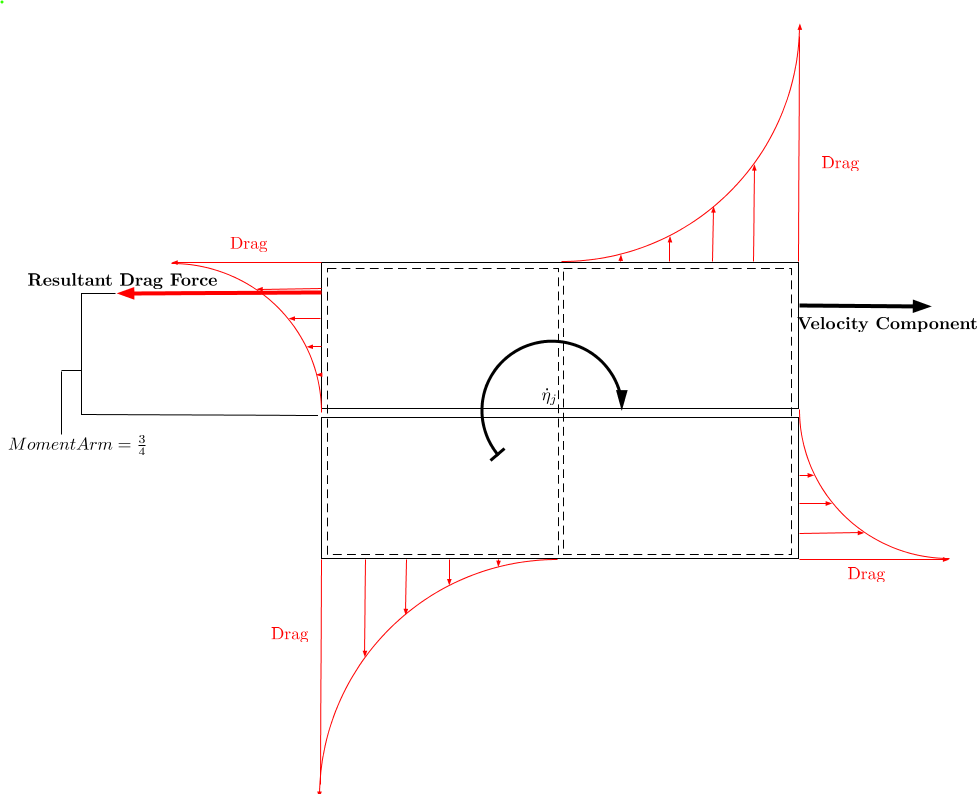
\includegraphics[width = 12cm]{figure/chap4/ROV_disc.jpg}
\bicaption[fig:chap4:F2]{ROV的阻尼力离散}{ROV的阻尼力离散}{Fig.}{Discretization of ROV damping\cite{eidsvik2015identification}}
\end{figure}

要估计旋转自由度中的非线性阻尼是相当具有挑战性的,主要是因为没有好的经验方法。 由于作者并不能够从别的资料找到一种可靠的方法来估计旋转自由度的非线性阻尼,就必须建立一种新方法来进行估算。这种方法建立在这个事实上,即小旋转可以将旋转运动等价为平移运动。

首先将ROV划分为围绕每个轴的总共4个象限(将所有3个轴共计加上12个象限)。此外,将假设每个象限仅在水平或垂直方向上移动。 通过查看图\ref{fig:chap4:F2},这意味着固体象限将水平移动,装订的象限将垂直移动。这里,最重要的假设是象限具有小角度旋转。

因为二次阻尼是相对于速度的二次函数,在象限靠近中心的位置阻尼为零,而在最外面则阻尼最大,可以参考图\ref{fig:chap4:F2}。力矩的力臂大约在象限内远离旋转中心中的$\frac{3}{4}$的位置处。旋转阻尼可以由每个象限的阻尼系数和局部的末端的平移速度来表示。

要表示旋转运动的阻尼,首先要确定不同象限的平移速度,不同自由度的平移速度表示如下:

\begin{equation}
\begin{aligned}
\overline{v_2} [m/s] = v_2 [rad/s] \ast \frac{(L/B/H)}{2}[m]
\end{aligned}
\end{equation}

每个象限的阻尼力系数需要查询文献论文中的表格\cite{eidsvik2015identification}。每个象限的阻尼力公式可以写为($om$ 是水平象限,$mn$是垂直象限):
\begin{equation}
\begin{aligned}
F_{quadrant}^{j} = \frac{1}{2} \ast \frac{1}{3} \ast \rho \ast C_D \ast A \ast  C_p^{om/mn} \ast  \lambda \overline{v_2} \ast | \overline{v_2}|, j = 4, 5, 6
\end{aligned}
\end{equation}

将每个象限的力乘以力臂就可以得到绕轴的力矩:


\begin{equation}
\begin{aligned}
 \overline{M}_{quad}^j= F_{quadrant}^{j} \ast \frac{3}{4} \frac{L,B,H}{2}
\end{aligned}
\end{equation}

再次说明的是,L,B或H取决于自由度以及它是否是水平的或垂直象限。

这样可以得到水平的速度:

\begin{equation}
\begin{aligned}
M_{quad}^{j} = \overline{M}_{quad}^{j} \ast (\frac{L,B,H}{2}) ^2
\end{aligned}
\end{equation}

将水平和垂直象限的阻尼加到一起就可以得到合阻尼力矩如下:

\begin{equation}
\begin{aligned}
M_{tot} = 2 \ast M_{quad-Horizontal}^{j}  + 2 \ast M_{quad-Vertical}^{j}
\end{aligned}
\end{equation}

对于线性阻尼,是很难进行分析估计的。虽然有很多的水面船的近似估计存在。对于水面船的线性摩擦阻尼,Fossen提出如下的经验公式:

\begin{equation}
\begin{aligned}
B_{11}^{LIN} &= \frac{M_{11} + A_{11}}{T_{surge}} \\
B_{22}^{LIN} &= \frac{M_{22} + A_{22}}{T_{sway}} \\
B_{33}^{LIN} &= 2 \Delta \zeta_{heave} \omega_{heave} [M_{33} + A_{33}(\omega_{heave})]\\
B_{44}^{LIN} &= 2 \Delta \zeta_{roll} \omega_{roll} [I_{44} + A_{44}(\omega_{roll})]\\
B_{55}^{LIN} &= 2 \Delta \zeta_{pitch} \omega_{pitch} [I_{55} + A_{55}(\omega_{pitch})]\\
B_{66}^{LIN} &= \frac{I_{66}+A_{66}}{T_{yaw}}
\end{aligned}
\end{equation}
其中,$T_{DOF} = \frac{T_n(DOF)}{2\Pi \zeta}$, $T_n(DOF)$是每个自由度的自然周期,$\zeta$是阻尼比。
本文中研究的是ROV,但可以采用水面船相类似的方法进行处理。首先,给出一阶粘性阻尼的自由振动方程:

\begin{equation}
\begin{aligned}
(m+m_a)\ddot{\overline{X}} + K_L \dot{\overline{X}} + g \overline{X} = 0
\end{aligned}
\end{equation}

除以ROV的质量并求得状态方程根如下:

\begin{equation}
\begin{aligned}
\left \{ \begin{matrix}
\lambda _1 \\
\lambda _2
\end{matrix} \right \}
=  - \frac{K_L}{2m}\pm \sqrt{K_L^2 - 4mg}
\end{aligned}
\end{equation}

那么可以得到临界阻尼为$K_{L} = 2m\omega_n$,将临界阻尼带入方程可得:

\begin{equation}
\begin{aligned}
\ddot{\overline{X}} + 2\zeta \omega_n \dot{\overline{X}} + \omega_n^2 \overline{X} = 0
\end{aligned}
\end{equation}
其中,
\begin{equation}
\zeta = \frac{K_L}{K_{L,critical}} = \frac{K_L}{2m\omega_n}
\end{equation}
这样就可以使用三个参数来估计线性阻尼。质量和自然频率可以被计算,但是阻尼比需要预先设定一个值。对于水面船,横滚自由度的阻尼比一般的范围是$2-10\%$。而对于ROV,阻尼比可设定为$2.5\%$。虽然这个阻尼比的值不能确定完全准确的值,但是它是在一个相对合理的范围内。

自然频率给出如下:

\begin{equation}
\begin{aligned}
\omega_n =  \sqrt{\frac{g}{m+m_a}}
\end{aligned}
\end{equation}

线性阻尼可得:
\begin{equation}
\begin{aligned}
K_L = 2 \zeta m \sqrt{\frac{g}{m+m_a}}
\end{aligned}
\end{equation}

由于恢复力的存在,线性阻尼在横滚和俯仰自由度内可使用这种方法来计算。假设俯仰自由度内,线性阻尼和二次阻尼的系数间存在一种比例关系,那么可使用缩放系数来从俯仰或者横滚自由度来获得偏航的阻尼。对于平移自由度缩放系数是0.16。

将上面的线性和非线性阻尼项加上一起就可以获得ROV的完全阻尼矩阵的估计。

\subsection{基于CFD的数值计算法}

本节中,将介绍一种使用流体数值计算软件来给水下机器人进行建模的方法。在前的一部分中,已经介绍了非初等几何类型的ROV的经验分析法,在本节中,所有的模型关键项都是基于CAD的模型已知的。刚体惯性质量矩阵可以使用CAD软件如CATIA进行测量,恢复力主要是在确定水下机器人的浮心和重心后,参考第二章水下机器人模型中对恢复力的定义确定。本节主要集中于使用CFD软件对附加质量和阻尼力项进行计算上。

\subsubsection{附加质量}

水下机器人形状会给附加质量带来影响,对于复杂形状的水下机器人,采用基本形状的船体进行预测和逼近的经验公式往往是不准确的。为了解决这个问题,使用WAMIT和AWQA软件可以计算水下机器人的附加质量项。在本文例子中,首先使用WAMIT的计算值作为对比,而使用AWQA海洋工程计算软件来完成对附加质量项的估计。

首先使用流体计算软件计算一个球体的附加质量,球体的附加质量的理论值为$2/3\pi \rho r^3$。球体的附加质量的理论值可以用来验证流体软件中计算附加质量的配置是否正确,计算的对比结果如表\ref{tab:chap4:table3-1},其中球体的直径为1m,密度为1kg/m3,水深为10m。

要计算水下机器人的附加质量,首先对水下机器人的模型进行简化预处理,以保证AQWA软件计算的质量和效率。AWQA是集成在ANSYS中的一款通用的流体动力学分析软件,可以使用ANSYS的网格预处理MESH模块建立网格,网格设计不要太密,也不要太少。网格太少会让计算的结果可行度降低,网格太密又会让计算时间很长,导致计算积累误差出现,计算的结果可信度也会降低。图\ref{fig:chap4:F3}显示3000m级别的工作性ROV在AWQA软件里的几何表示图。

\begin{table}
\centering
\label{tab:chap4:table3-1}
\bicaption[tab:chap4:table3-1]{球体附加质量}{球体附加质量}{Table}{Added mass of a sphere}
\begin{tabular}{cccc}
\toprule
           & Theoretical & WAMIT     & AWQA     \\
\midrule
 Surge(kg) & 2.0944      & 2.084236  &2.1406    \\
\bottomrule
\end{tabular}
\end{table}

\begin{figure}
\label{fig:chap4:F3}
\centering
\subfigure[CATIA中模型简化]{
\label{fig:chap4:F3a}
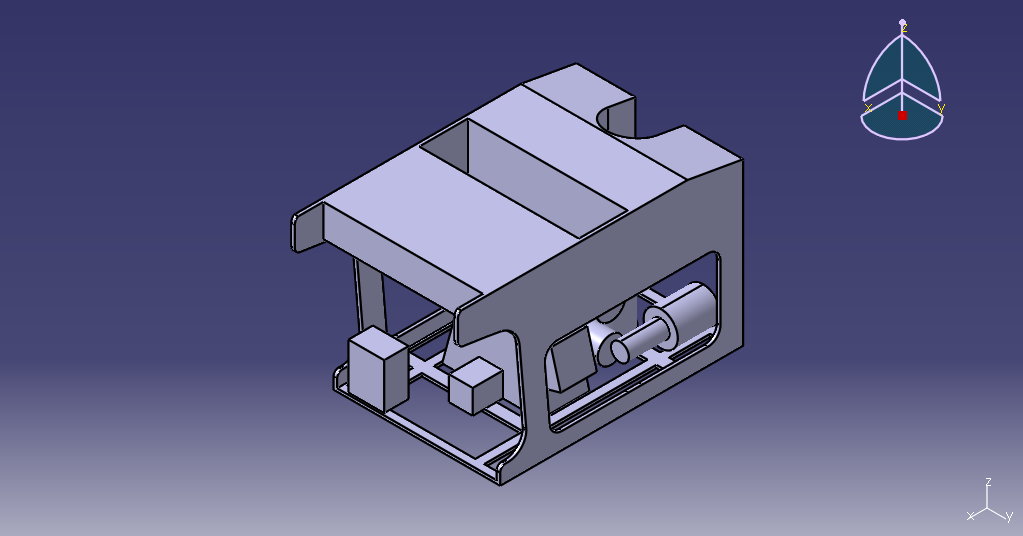
\includegraphics[width = 13cm]{figure/chap4/catia_aqwa.png}
}
\subfigure[AQWA中模型网格]{
\label{fig:chap4:F3b}
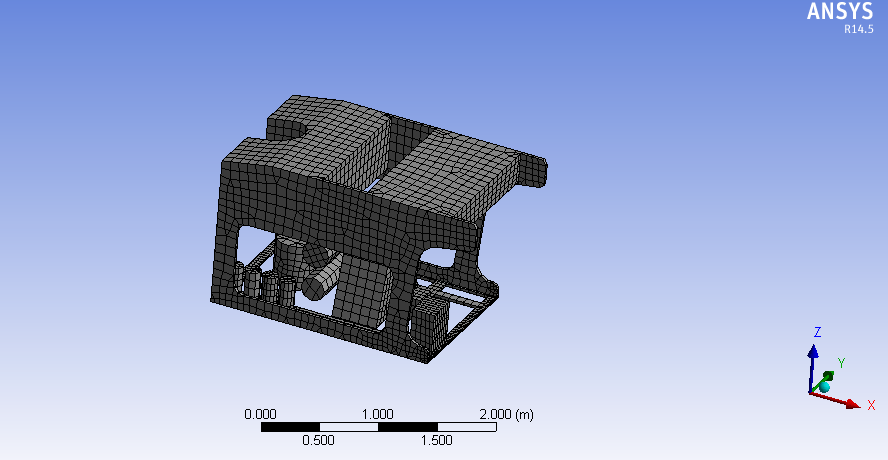
\includegraphics[width = 13cm]{figure/chap4/aqwa_mesh.png}
}
\bicaption[fig:chap4:F3]{ROV简化与网格模型几何表示}{ROV简化与网格模型几何表示}{Fig.}{Geometric representation of ROV in AWQA and CATIA}
\end{figure}


AQWA软件中的设置条件如下:水下机器人为水下5m的水深处,海水密度为1025$kg/m^3$, 水深100m, 水域为正方形($100\times100m$),波浪周期范围为1-125.664秒, 波浪频率范围为0.008-1Hz,波浪方向为水平面内-180-180度且间隔为45度的8个方向, 结合计算机的配置,网格节点数为5468,网格大小范围为15mm-150mm。

由于使用AWQA计算附加质量需要确定刚度质量矩阵,使用CATIA软件可以获得3000m水下机器人的$M_RB$如下:

\begin{equation}
\begin{aligned}
M_{RB} = \begin{bmatrix}
   1468&0   &0   &0&0&0 \\
     0 &1468&0   &0&0&0 \\
     0 &0   &1468&0&0&0 \\
     0 &0   &0   &428.777 &-19.904 &-0.815\\
     0 &0   &0   &-19.904&819.483 &0.473  \\
     0 &0   &0   &-0.815 &0.473   &775.496
         \end{bmatrix}
\end{aligned}
\end{equation}

\subsubsection{阻尼力}

水下机器人受到流体阻尼力主要分为线性阻尼和非线性阻尼。两种阻尼都和水下机器人的运行速度有关,由于水下机器人运行的速度范围内两种阻尼都存在,为了精确地估计水下机器人受到的阻尼力,本节选择使用STAR CCM+ 流体计算软件对水下机器人,如3000m级别ROV,进行量化阻尼分析。除了前一节本文介绍的经验估算法,二次阻尼也可以采用如下公式进行粗略的确定阻尼行为。二次阻尼表示如下:

\begin{equation}
\begin{aligned}
f(U)=-\frac{1}{2}\rho_d C_D(R_n)AU|U|
\end{aligned}
\end{equation}
其中,$U$是机器人运行速度,$\rho_{d}$是流体密度,$A$是投影的横截面积,$C_D(R_n)$是阻尼系数,该系数与雷诺数$R_{n}$有关。

本部分是采用CFD流体计算软件进行阻尼分析,但又结合水下机器人建模目的是用于控制的,因此仅需要根据控制目标对ROV的受控自由度进行阻尼分析。采用STAR CCM+流体计算软件对深水ROV模型进行阻尼分析,主要分为纵荡、垂荡、偏航自动度的流体计算的阻尼分析。平移运动如垂荡自由度的阻尼分析设置需给出运行速度范围、网格设置以及边界层设置。

以前进计算为例,在来流方向,计算域取10倍的ROV长度,前端网格长度为ROV的长度的3倍,后端网格长度为ROV长度的7倍;在宽度方向上,整体网格宽度取ROV宽度的5倍;使用STAR CCM+进行网格划分,计算域内的网格模型为TRIM模型,在ROV周围采取加密措施,保证流动细节的捕捉,生成的体网格的数量为332万,网格显示如图\ref{fig:chap4:F4}。边界条件设置:设置入口速度边界,大小为0-1.5m/s,出口设置为压力出口,壁面采用无滑移边界。湍流模型采用Realizable K-Epsilon Two-layer(RKE)模型,边界层处理采用Two-layer all y与wall treatment。湍流强度为0.05,湍流尺度为0.1m,边界层增长率为1.2。上浮计算的例子也与前进的计算例子类似,在高度方向,网格长度是10的ROV长度,网格类型是TRIM,网格数量为330万,在ROV的周围采取加密措施,入口速度大小为0-1m/s。前进计算的速度矢量图和力收敛显示如图\ref{fig:chap4:F5},表示数值计算是成功的。

对于偏航旋转计算,旋转的计算域有两个区域,其中有一个是旋转域,外部区域的长度和宽度一致,为ROV的10倍,中间旋转域直径为ROV的长度1倍,旋转域采用的模型是运动参考坐标系(MRF)。ROV的旋转速度设置为0-1.5rad/s,网格数量为,网格类型为TRIM。边界层设置参考前进计算例子进行设置。
偏航自由度旋转运动的计算域网格如图\ref{fig:chap4:F6}。

\begin{figure}
\label{fig:chap4:F4}
\centering
\subfigure[]{
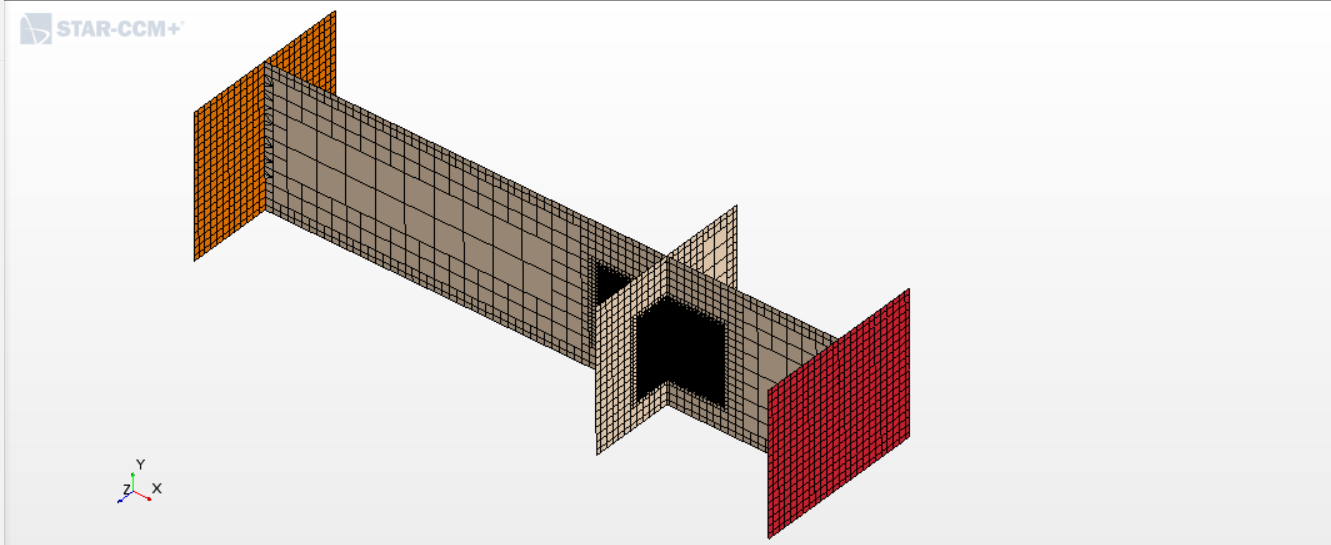
\includegraphics[width = 15cm]{figure/chap4/mesh1.png}
}
\subfigure[]{
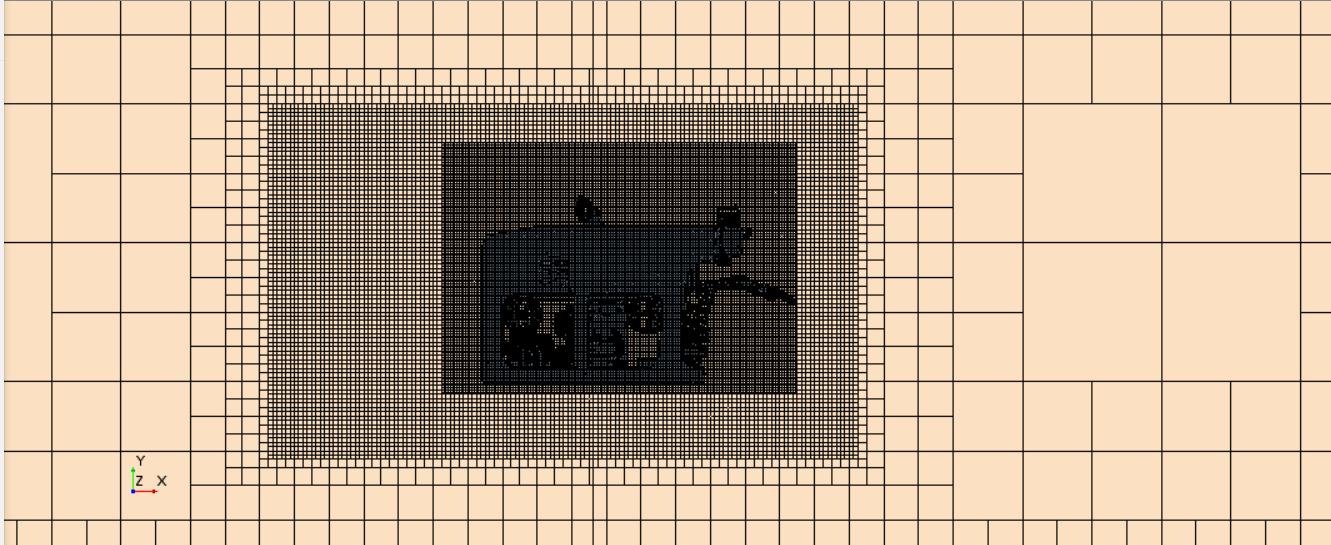
\includegraphics[width = 15cm]{figure/chap4/mesh2.png}
}
\bicaption[fig:chap4:F4]{纵荡运动网格}{纵荡运动网格}{Fig.}{The mesh of ROV surge motion}
\end{figure}

\begin{figure}
\label{fig:chap4:F5}
\centering
\subfigure[]{
\includegraphics[width = 15cm]{figure/chap4/rov_surge1.png}
}
\subfigure[]{
\includegraphics[width = 15cm]{figure/chap4/rov_surge2.png}
}
\bicaption[fig:chap4:F5]{纵荡运动分析与阻力}{纵荡运动分析与阻力}{Fig.}{ROV surge analysis and damping force}
\end{figure}




\begin{figure}
\label{fig:chap4:F6}
\centering
\subfigure[]{
\includegraphics[width = 10cm]{figure/chap4/mesh3.png}
}
\subfigure[]{
\includegraphics[width = 10cm]{figure/chap4/mesh4.png}
}
\bicaption[fig:chap4:F6]{偏航运动网格}{偏航运动网格}{Fig.}{The mesh of ROV yaw motion}
\end{figure}


\subsection{结果与分析 }

本节首先介绍经验法和流体数值计算方法来估算3000m的深海ROV的模型的流体动力学参数。
经验法相关的参数如下:水下机器人的长度$L=2480[mm]$,高度$H=1630[mm]$,宽度$W=1400[mm]$,水流密度为$1000[kg/m^3]$, 正视图投影面积$PF= 1.92 \times 10^6[mm^2]$,侧视图投影面积$PS= 2.782 \times 10^6[mm^2]$, 上视图投影面积$PT= 2.215\times 10^6[mm^2]$,俯仰和横滚自由度的恢复力系数$C_p = 5697$,线性和非线性的阻尼缩放系数$\lambda = 0.16$。

经过经验法的附加质量和阻尼力计算程序的运行计算,可以得到结果如下:

附加质量项
\begin{equation}
\begin{aligned}
\bm{M_{A}} = \begin{bmatrix}
   1014.070&0   &0   &0&0&0 \\
     0 &2143.288&0   &0&0&0 \\
     0 &0   &1706.464&0&0&0 \\
     0 &0   &0   &242.965 &0 &0\\
     0 &0   &0   &0 & 671.014 &0 \\
     0 &0   &0   &0 &0   &543.627
         \end{bmatrix}
\end{aligned}
\end{equation}

阻尼力项$\bm{D}$包括线性阻尼$\bm{D_L}$和非线性阻尼$\bm{D_N}$,且满足如下公式
\begin{equation}
\begin{aligned}
\bm{D} = \bm{D_L} + \bm{D_N}\nu
\end{aligned}
\end{equation}

线性阻尼项结果
\begin{equation}
\begin{aligned}
\bm{D_L} = \begin{bmatrix}
   148.153&0   &0   &0&0&0 \\
     0 &273.998&0   &0&0&0 \\
     0 &0   &197.270&0&0&0 \\
     0 &0   &0   &97.815 &0 &0\\
     0 &0   &0   &0 & 145.699 &0 \\
     0 &0   &0   &0 &0   &178.869
         \end{bmatrix}
\end{aligned}
\end{equation}

非线性阻尼项结果
\begin{equation}
\begin{aligned}
\bm{D_N} = \begin{bmatrix}
   925.958&0   &0   &0&0&0 \\
     0 &1712.486&0   &0&0&0 \\
     0 &0   &1232.940&0&0&0 \\
     0 &0   &0   &254.366 &0 &0\\
     0 &0   &0   &0 & 652.675 &0 \\
     0 &0   &0   &0 &0   &801.264
         \end{bmatrix}
\end{aligned}
\end{equation}

使用STAR CCM+软件分别对纵荡、垂荡、偏航自由度进行阻尼分析,可以得阻尼力结果如表\ref{tab:chap4:table3-2}、表\ref{tab:chap4:table3-3}和表\ref{tab:chap4:table3-4}所示。计算的纵荡、垂荡速度流线图结果可以见图\ref{fig:chap4:F7}和图\ref{fig:chap4:F8}。图\ref{fig:chap4:F9}给出了偏航旋转运动的矢量图和速度线图。采用二阶多项式来对阻尼力数据进行拟合分别对纵荡、垂荡、偏航三个模式的阻尼力进行拟合,这可以得到速度和阻尼力之间的关系,分别如图\ref{fig:chap4:F10}、图\ref{fig:chap4:F11}和图\ref{fig:chap4:F12}。


\begin{table}
\centering
\label{tab:chap4:table3-2}
\bicaption[tab:chap4:table3-2]{纵荡自由度阻尼分析}{纵荡自由度阻尼分析}{Table}{ROV surge damping}
\begin{tabular}{ccccccc}
\toprule
 Velocity(m/s)    & 0.3 & 0.6 & 0.9 &1.2  &1.5   \\
\midrule
 Damping force(N) & 99.9 &398 &905 & 1610 & 2520  \\
\bottomrule
\end{tabular}
\end{table}

\begin{table}
\centering
\label{tab:chap4:table3-3}
\bicaption[tab:chap4:table3-3]{垂荡自由度阻尼分析}{垂荡自由度阻尼分析}{Table}{ROV heave damping}
\begin{tabular}{ccccc}
\toprule
 Velocity(m/s)    & 0.25   & 0.5 & 0.75    &1     \\
\midrule
 Damping force(N) & 111    & 448 & 1003.56 & 1780 \\
\bottomrule
\end{tabular}
\end{table}

\begin{table}
\centering
\label{tab:chap4:table3-4}
\bicaption[tab:chap4:table3-4]{偏航自由度阻尼分析}{偏航自由度阻尼分析}{Table}{ROV yaw damping}
\begin{tabular}{cccccc}
\toprule
 Velocity(rad/s)    & 0.3   & 0.6 & 0.9  &1.2   & 1.5   \\
\midrule
 Damping torque(Nm) & 142.4 & 633 & 1392 & 2442 &3958    \\
\bottomrule
\end{tabular}
\end{table}

\begin{figure}
\label{fig:chap4:F7}
\centering
\subfigure[]{
\includegraphics[width = 15cm]{figure/chap4/rov_surge3.png}
}
\subfigure[]{
\includegraphics[width = 15cm]{figure/chap4/rov_surge4.png}
}
\bicaption[fig:chap4:F7]{ROV前进速度为1.5m/s时速度流线和矢量图}{ROV前进速度为1.5m/s时速度流线和矢量图}{Fig.}{ Speed streamline and vector diagram for ROV with surge speed 1.5m/s}
\end{figure}


\begin{figure}
\label{fig:chap4:F8}
\centering
\subfigure[]{
\includegraphics[width = 10cm]{figure/chap4/rov_up1.png}
}
\subfigure[]{
\includegraphics[width = 10cm]{figure/chap4/rov_up2.png}
}
\bicaption[fig:chap4:F8]{ROV上浮速度为0.5m/s时速度流线和矢量图}{ROV上浮速度为0.5m/s时速度流线和矢量图}{Fig.}{ Speed streamline and vector diagram for ROV with floating speed 0.5m/s}
\end{figure}


\begin{figure}
\label{fig:chap4:F9}
\centering
\subfigure[]{
\includegraphics[width = 10cm]{figure/chap4/rov_yaw1.png}
}
\subfigure[]{
\includegraphics[width = 10cm]{figure/chap4/rov_yaw2.png}
}
\bicaption[fig:chap4:F9]{ROV偏航速度为1.5rad/s时速度流线图和矢量图}{ROV偏航速度为1.5rad/s时速度流线图和矢量图}{Fig.}{ Speed streamline and vector diagram for ROV with yaw rate 1.5rad/s}
\end{figure}

\begin{figure}
\label{fig:chap4:F10}
\centering
\includegraphics[width = 10cm]{figure/chap4/damping_surge.png}
\bicaption[fig:chap4:F10]{ROV的纵荡自由度的经验法和数值分析拟合结果对比}{ROV的纵荡自由度的经验法和数值分析拟合结果对比}{Fig.}{ Comparision between empirical method and numerical analysis in the ROV's surge channel}
\end{figure}

\begin{figure}
\label{fig:chap4:F11}
\centering
\includegraphics[width = 10cm]{figure/chap4/damping_heave.png}
\bicaption[fig:chap4:F11]{ROV的垂荡自由度的经验法和数值分析拟合结果对比}{ROV的垂荡自由度的经验法和数值分析拟合结果对比}{Fig.}{ Comparision between empirical method and numerical analysis in the ROV's heave channel}
\end{figure}

\begin{figure}
\label{fig:chap4:F12}
\centering
\includegraphics[width = 10cm]{figure/chap4/damping_yaw.png}
\bicaption[fig:chap4:F12]{ROV的偏航自由度的经验法和数值分析拟合结果对比}{ROV的偏航自由度的经验法和数值分析拟合结果对比}{Fig.}{ Comparision between empirical method and numerical analysis in the ROV's yaw channel}
\end{figure}


采用AQWA软件和STAR CCM+软件分别预测附加质量项和阻尼力的估计方程,结果如下:

附加质量:

\begin{equation}
\begin{aligned}
\bm{M_{A}} = \begin{bmatrix}
     877.31 &   5.5756 &  -114.49 &  -1.8992 &   447.47 &   3.9657\\
     4.8538 &   1432.8 &  -1.4758 &  -468.2  &   6.0126 &    361.5\\
     -115.54 &  -5.9954  &  1763  &  -4.8197 &  -693.41 &  -5.3964\\
     -0.78241 &  -490.1  &  -1.8668  &  539.36 & 2.6651  &  -140.62\\
     452.9  &  6.195 &  -694.04  &  3.5358 &   1160.4  & -0.77008\\
     2.4616  &  355.83 &  -3.8789 &  -130.34 &  -0.94418  &  598.42\\
         \end{bmatrix}
\end{aligned}
\end{equation}


将经验法和数值分析方法获得附加质量进行对比,可以发现两者之间存在着一致性。对于阻尼项,通过分析两种不同方法计算的阻尼力预测值对比结果,可以看出虽然经验法和数值计算法两者之间存在一定的差异,但是也在数量级上具有一致性,可以验证本节给出的两种方法的有效性。


\section{基于泰勒公式简化的水下机器人模型建立  }

控制导向的水下机器人建模,在水下机器人数学模型描述未知时,可以采用经验法和数值分析法预测水动力模型参数。然而在有些水下机器人案例中,水下机器人的模型是基于潜艇、鱼雷模型以及舵片经验数据来确定的\cite{yuanchuan2001submarine,Borst1985Fluid,bottaccini1954stablity}。在水下机器人的数学模型描述已知但是却非线性耦合非常严重时,就需要基于控制目标进行数学处理。

经常用于模型参考自适应控制应用中的水下机器人系统模型可以根据系统的模型形式分为线性系统和非线性系统。 然而,大多数模型参考自适应控制中引入的线性系统模型是通过忽略航行器系统中的高阶或非线性项而从实际航行器中推导出来的。通过理论和经验数据相结合的REMUS 100 AUV的6自由度(DOF)非线性系统模型为改善REMUS的控制提供了更精确的航行器平台。

REMUS AUV的非线性模型的高度复杂性,对于后续的控制带来了很大挑战。 REMUS AUV模型是总结实验数据而建立的非线性模型,它对于研究AUV的动力学的性能和控制器设计都非常重要,但是由于其建立是从动力学分析角度建立的,并不完全适用于控制应用。AUV水下机器人多是由舵片和推进器共同驱动,但由于舵片本身的工作空间受限制,且该类型的水下机器人多是系统控制输入数目小于系统自由度的,因此在进行位置和姿态控制的时候,仅仅选择其中几个关键量进行控制。

本节选择以控制俯仰姿态为目标,从水下机器人的6自由度运动动力学模型中提取出俯仰姿态的控制方程:
\begin{equation}
\label{depth_equ}
\begin{array}{l}
 z =  - {\rm{sin}}\theta u + \cos \theta \sin \varphi v + \cos \theta \cos \varphi \omega  \\
 {I_y}\dot q + ({I_x} - {I_z})rp + m[{z_G}(\dot u - vr + \omega q) - {x_G}(\dot \omega  - uq + vp)] =  - ({z_G}W - {z_B}B)\sin \theta  \\
 \begin{array}{*{20}{c}}
   {} & {}  \\
\end{array} - ({x_G}W - {x_B}B)\cos \theta \cos \varphi  + {M_{\omega \left| \omega  \right|}}\omega \left| \omega  \right| + {M_{q\left| q \right|}}q\left| q \right| + {M_{\dot \omega }}\dot \omega  + M_{\dot q}^{}q + {M_{uq}}uq \\
 \begin{array}{*{20}{c}}
   {} & {}  \\
\end{array} + {M_{vp}}vp + {M_{rp}}rp + {M_{u\omega }}u\omega  + {M_{uu\delta }}{u^2}{\delta _e} \\
 \theta  = \cos \varphi q - \sin \varphi r \\
 \end{array}
\end{equation}
其中 $\delta_e$ 是水平舵片输入角。

为了获得控制用的方程,方程可以在操作点$\theta_0$, $q_0$, $u_0$, $z_0$ 使用泰勒公式进行展开,并忽略其中的高阶项,则可以得到简化后的模型如下:

\begin{equation}
\begin{array}{l}
 z =  - {u_0}\cos {\theta _0}\theta  \\
 {I_y}\dot q + m{x_G}{u_0}q =  - ({z_G}W - {z_B}B)\cos {\theta _0}\theta  \\
 \begin{array}{*{20}{c}}
   {\begin{array}{*{20}{c}}
   {} & {}  \\
\end{array}}  \\
\end{array} + ({x_G}W - {x_B}B)\sin {\theta _0}\theta  + 2{M_{\left| q \right|q}}\left| {{q_0}} \right|q \\
 \begin{array}{*{20}{c}}
   {\begin{array}{*{20}{c}}
   {} & {}  \\
\end{array}}  \\
\end{array} + {M_{\dot q}}\dot q + {M_{uq}}{u_0}q + {M_{uu\delta }}u_0^2{\delta _e} \\
 \dot \theta  = q \\
 \end{array}
\end{equation}

简化后的方程被转为带有不确定性的状态方程的形式:

\begin{equation}
\begin{array}{l}
 \left[ {\begin{array}{*{20}{c}}
   {\dot \theta }  \\
   {\dot q}  \\
\end{array}} \right] = \left[ {\begin{array}{*{20}{c}}
   0 & 1  \\
   {\frac{{ - ({z_G}W - {z_B}B)\cos {\theta _0}}}{{{I_y} - {M_{\dot q}}}}} & {\frac{{ - m{x_G}u_0^{} + 2{M_{q\left| q \right|}}\left| {{q_0}} \right| + {M_{uq}}{u_0}}}{{{I_y} - {M_{\dot q}}}}}  \\
\end{array}} \right]\left[ {\begin{array}{*{20}{c}}
   \theta   \\
   q  \\
\end{array}} \right] + \left[ {\begin{array}{*{20}{c}}
   0  \\
   {\frac{{{M_{uu\delta }}{u_0}^2}}{{{I_y} - {M_{\dot q}}}}}  \\
\end{array}} \right]{\delta _e} \\
 \begin{array}{*{20}{c}}
   {} & { + \frac{1}{{{I_y} - {M_{\dot q}}}}\left[ {\begin{array}{*{20}{c}}
   0 & 0 & 0  \\
   \gamma  & \lambda  & \zeta   \\
\end{array}} \right]}  \\
\end{array}\left[ {\begin{array}{*{20}{c}}
   u  \\
   q  \\
   \theta   \\
\end{array}} \right] \\
 \end{array}
\end{equation}
其中, $\gamma$,$\lambda$,$\zeta$ 是与$u$, $q$, $\theta$相关的不确定性系数。此外,横滚自由度的横滚角$\varphi$、速度$p$在方程中是被视为干扰的。

采用本节的非线性模型简化方法,可以获得用于控制的参考模型方程,对于其他的自由度,也可以参考与此类似的方法进行处理。

\section{本章小结 }

本章系统地研究了水下机器人的用于鲁棒自适应控制的建模问题。水下机器人的种类不同,模型确定方法也有差异,用于控制目标的水下机器人建模,不必非常精确,但是应能表征水下机器人所要控制模式的主要部分。本章分别从水下机器人外形、数学模型两个角度对水下机器人进行建模。基于机器人外形而进行的建模主要分为经验法和流体软件数值分析法,以上方法可适用于具有非初等几何外形的ROV,而具有流线型且已知非线性模型的AUV,可以以控制目标为导向对模型进行数学简化,并分析控制模型的不确定性。首先,考虑到水下机器人的模型未知且实验数据不可获取,仅仅具有水下机器人的一些设置功能要求以及物理模型等资料,尤其对于非初等几何表面的低速水下机器人,通过分析水下机器人动力学模型的各个项的重要性,简化动力学模型,并确定了附加质量和非线性阻尼为主要计算项。经验法主要基于实验数据的总结,可以对水动力参数进行相对精确的快速估算。数值分析方法主要使用流体计算软件STAR CCM+和ANSYS/AWQA软件分别求取模型关键参数和提取重要的数据。其次,针对水下机器人非线性精确模型已知,对运动方程进行解耦,并进行泰勒展开,确定可以用于自适应控制的参考模型,本章给出了俯仰模式的泰勒展开模型。本章给出的方法从多个角度为水下机器人进行建模,最大程度了方便了控制应用。

%# -*- coding:utf-8 -*-
%!TEX root = ../thesis.tex



\chapter{水下机器人的鲁棒自适应控制}

\label{chap:robust_adaptive}
% 5.1 引言
% 5.2 水下机器人的控制特性
% 5.2.1 水下机器人控制中的自适应性
% 5.2.2 水下机器人控制中的鲁棒性
% 5.2.3 水下机器人应用中的驱动器非线性
% 5.3 鲁棒自适应控制与系统稳定性
% 5.4 模型参考自适应控制
% 5.4.1 模型参考自适应的水下机器人控制
% 5.4.2 基于射影理论的模型参考自适应控制
% 5.4.3 L1AC 自适应控制
% 5.4.4 仿真结果与分析
% 5.5 本章小结


\section{引言 }
水下机器人系统本质上是非线性的,这与许多物理系统一样,水下机器人系统复杂,包括动力学系统、控制系统、观通系统。实际水下机器人系统中,非线性是根据成因不同分为人为非线性和自然非线性。固有非线性不仅包含由于运动导致的非线性也包括高阶的非线性耦合。不可观测的状态量导致了水下机器人测量系统中的非线性出现,这一部分可以由人为设定,也可以是系统本身的固有特性。驱动器也具有非线性特点,不过非线性的判定对于一个小范围运行的系统取决于非线性的大小和对系统的性能影响大小。就水下机器人的模型本身而言,不确定性也是影响水下机器人系统正常工作的重要因素。水下机器人的模型包括模型的数学结构和数学模型中的各项参数。非线性自适应控制是一种典型模型参考型自适应控制,但是参考的模型的往往并不是准确的,一部分是由于模型的结构参数估计有偏差,另一部分是由于模型中可能存在的未建模动力学。时间演化会给水下机器人系统带来参数不确定性,也可能会给水下机器人的模型结构带来新的变化。水下机器人的控制器要能够应对水下机器人中的各种问题,就需要控制器能够自适应地更新参考模型,并尽量克服不确定性、干扰带来的状态偏差。控制器要应对变化就可能会因高增益、快速自适应、高频信号出现不稳定的问题。因此,自适应和鲁棒性是水下机器人控制器设计中需要重点关注的问题,也是本章提出鲁棒自适应控制的原因。

鲁棒自适应控制的理解可以从两个方面展开,一个是鲁棒控制的必要性,一个是自适应控制的必要性。鲁棒控制是为应对包含有界不确定性系统而开发的一种在线的控制方法。鲁棒控制是使用反馈信号和前馈命令来产生相应的控制命令,从而让水下机器人能够跟踪预定的指令。鲁棒控制的主要目标是为应对水下机器人在系统动态运动时发生不可以预见的意外情况,而能让系统可以保持正常工作而不出现故障。

水下机器人的研究是从建模展开的,求出水下机器人的控制用数学模型。虽然使用系统辨识或者控制导向建模的经验法或者流体数值预测方法可以获得参考模型,但是获得的模型可能是不准确的,模型本身会存在潜在的缺陷。鲁棒控制可以在水下机器人系统出现不确定性时,让系统响应平滑而保持稳定,这种方法对于系统中出现小程度的意外状况时尤其有效,可以确保控制系统不会崩溃失效。水下机器人工作的水下环境会给系统带来不确定性,在有限可控的变化范围内,使用鲁棒控制可以确保控制系统的闭环稳定性和对意外情况的容忍性。

鲁棒控制可以用来应对一定的不确定性变化,但是文中追求的控制是能否将鲁棒控制可以应对的不确定性的范围扩大,涵盖更多的系统动态变化。非线性自适应控制可以用来解决很多不确定性的问题,包括结构不确定性、参数不确定性还有非线性。自适应控制的方法好像满足了文中提出的控制目标,能够应对较多的不确定性,但也这里需要回归到非线性自适应控制的方法本身再来判断。针对具有结构不确定性,参数不确定性和非线性的动态系统模型,设计出状态模型参考自适应控制器,但是自适应控制的自适应律是没有边界的且容易受到多种因素的影响,尤其是有界干扰的影响。为了保证非线自适应控制的鲁棒性,引入射影理论,确保自适应更新速率和自适应参数的一致有界,并确保闭环动态系统的误差和李雅普诺夫函数为负。使用射影算子修正状态模型参考自适应控制的自适应更新律就得到了鲁棒模型参考自适应控制方法,该方法可以保证系统的稳定性,也可以适应水下机器人系统中不确定性变化。

鲁棒模型参考自适应控制可以采用大量的动作行为来调节系统状态,也可以对自适应过程中的动态不确定性进行在线学习,以产生合理的控制输入来调整水下机器人的实际运行状态。不过,基于模型参考自适应控制的方法存在一定的缺陷,这种缺陷一方面来自于自适应本身牺牲速率作为代价,另一方面来自于自适应与鲁棒性的耦合。$L_1$自适应控制方法也是一种具有射影算子修正自适应律的控制方法,该方法可以同时更新参考模型与自适应律,并且将鲁棒性从自适应中解耦了出来。

水下机器人的俯仰控制具有高度非线性和不确定性,并且是一种静态不平衡系统,本文将鲁棒模型参考自适应控制方法和$L_1$自适应控制方法分别应用于水下机器人的姿态控制,以验证鲁棒自适应控制的可行性。需要说明鲁棒自适应控制并非应对所用控制问题的万能选择,它仅仅针对一般过程不确定性而设计。在水下机器人中,鲁棒控制和自适应控制都被分别应用,但鲁棒自适应控制才是设计一种好的控制方法的诀窍。

\section{水下机器人的系统控制特性 }

水下机器人系统复杂并随着时间而不断演化。水下机器人系统可以分为水下机器人的运动动力学模型和控制系统模型。首先,水下机器人系统根据系统的描述形式主要分为线性系统和非线性系统。其次,本节根据动力学模型与控制器的关系,给出水下机器人的模型不确定性与控制的关系。


\subsection{水下机器人的系统非线性 }
% 包括高阶项和各个自由度的耦合
% \subsection{水下机器人系统的 状态受限 }
% \subsection{水下机器人的输出大于输入的动态 特性}

物理系统本质上是非线性的。因此,水下机器人系统也不例外,水下机器人的控制器也存在一定程度上的非线性。非线性控制系统可以用非线性微分方程来描述。但是如果控制系统的工作范围比较小,并且在所涉及的非线性区间内是连续光滑的,这时控制系统可以通过一个线性化系统组合的近似系统来描述,其中每个线性系统的系统动力学可以使用一系列的线性微分方程来描述。

非线性系统的可以分为固有的非线性和人为的非线性。固有的非线性是系统的硬件和系统的运动自然产生。固有的非线性比如水下机器人旋转运动的科氏力和流体阻尼力。通常这种非线性很难被准确描述,也会对运动的控制带来不利影响,控制系统必须具有应对以上非线性的能力,比如设计合适的补偿器或者观测器。另外,人为的非线性是由设计者有意识的引入的,比如非线性控制系统中,设计者使用的非线性控制,是人为非线性的典型例子。水下机器人的实际系统中,固有非线性和人为非线性都存在。水下机器人的固有非线性根据运动模式除了包含阻尼非线性与旋转运动带来的科氏力,还包括水下机器人动力模型系统中的高阶项和系统各个自由度的非线性项耦合。此外,水下机器人的驱动系统、测量单元也具有自身的分线性的特性。需要说明,小范围运行的系统是否被视为线性或非线性系统取决于非线性的大小和对系统的性能影响程度。

水下机器人工作在未知的水下环境,其系统的非线性行为更复杂和多样性。从数学描述的角度,与线性方程不同,非线性方程通常不能通过分析来解决,此外传统的分析工具,如拉普拉斯变换,并不适用于非线性系统,这都是水下机器人的控制设计需要注意的问题。


\subsection{水下机器人模型不确定性 }

理解和估计模型中的相关不确定性对正确地认识水下机器人的运动机理和设计合适的控制器至关重要。水下机器人的模型包括模型的数学描述结构以及数学描述中的各项数学参数。在第三章的模型结构探索部分,可以发现数学的模型一方面来自于人类的现有认识,另一方面也可以采用启发式学习方法去搜索机器人模型中的新组成结构。合适的水下机器人的控制器不仅可以让机器人具有应对干扰的能力,还可以自动地适应来自于水下机器人自身模型与环境所带来的变化。水下机器人的模型变化从形式不同,可以分为参数的时间演化以及模型的结构演化。参数的时间演化给控制带来的问题即是参数不确定性,合理的控制器要能够自动更新控制律以应对参数不确定性带来的干扰。模型的结构演化较参数演化更为复杂,一种是在控制器设计的时候控制器的非线性估计部分存在未被建模的动力学,另一种是在时间的演化工程中水下机器人的模型结构出现了新的变化。两种不确定性都给控制器设计带来了挑战,控制器的设计既要能对工作过程中的不确定性进行在线估计,以尽量克服不确定性带来不利偏差。此外,对于控制器因设计不可以预测变化所带来的工作意外情况,也需要稳定地应对。

\section{鲁棒自适应控制框架 }

鲁棒自适应控制对那些存在不确定性的系统进行控制,首先要在控制系统的运行过程中,通过不断测量系统的输入、状态、输出或性能参数,逐渐了解和掌握对象,然后根据得到的过程信息,按一定的设计方法,作出控制决策去更新控制器的结构、参数,使系统在存在扰动和建模误差特性的条件下,系统仍能保持其稳定性和性能即具有鲁棒性,同时在某种意义下使控制效果达到最优或次优。为达到某个预期目标,按此设计思想建立的控制便是鲁棒自适应控制。为探索鲁棒自适应控制的必要性,需要首先分析自适应控制中存在的一些问题,本部分以模型参考自适应控制为例。

\subsection{Lyapunov稳定性 }

控制和系统理论里的一个核心点就是平衡点,首先给出非自治、非受迫动力学系统:
\begin{equation}
\dot x = f(t,x)
\end{equation}
其中,矢量函数\[ f:[0, \infty] \times D \rightarrow R^n\] 是一个分段连续的且在x上局部满足Lipschitz条件;具有一个包含原点x=0的域$D\subset R^n$。

\begin{defn}
对于非受迫且非自治系统,原点$x=0$是$t_0 =0$的一个平衡点,如果
\begin{equation}
f(t,0)=0 ,\quad \forall t \geqslant 0
\end{equation}
\end{defn}

一个动态系统,可以有很多个平衡点,有时这些平衡点是彼此孤立的,有时会连在一起,成为一串平衡点。当动态系统到达一个平衡点后,系统会一直停留在平衡点。

\begin{defn}[李亚普诺夫平衡稳定性]
如果对于任意$\varepsilon >0$ 和 $t_0 \geqslant 0$, 存在$\delta(\varepsilon ,t_0)>0$ 对所有初始条件$\left \| x(t_0) \right \| < \delta$ 和 $t \geq t_0 \geq 0$,相应的系统轨迹是有界的,那么非自治、受迫系统在平衡点是稳定的。如果平衡点是稳定的且$\delta$不取决于$t_0$,那么,平衡点是一致稳定的。最终,如果平衡点是不稳定的,那么平衡点是不稳定的。正式的定义如下:

稳定\\
$\forall \varepsilon >0$, $\forall t_0 >0$, $\exists \delta(\varepsilon,t_0)>0$, $\forall t \geqslant t_0$, $\left \| x(t_0) \right \| < \delta(\varepsilon,t_0) \Rightarrow \left \|  x(t) \right \| <\varepsilon$

一致稳定\\
$\forall \varepsilon >0$, $\forall t_0 >0$, $\exists \delta(\varepsilon)>0$, $\forall t \geqslant t_0$, $\left \| x(t_0) \right \| < \delta(\varepsilon) \Rightarrow \left \|  x(t) \right \| <\varepsilon$

不稳定\\
$\forall \varepsilon >0$, $\exists t_0 >0 $, $\forall \delta>0$, $\exists T\geqslant t_0$, $\left \| x(t_0) \right \| < \delta \Rightarrow \left \|  x(T) \right \| <\varepsilon$
\end{defn}

\begin{defn}[全局稳定性]
原点是全局稳定的,如果他是稳定的,且$\lim_{ \varepsilon \rightarrow \infty} {\delta}(\varepsilon ,t_0)= \infty$。
\end{defn}

\begin{defn}[渐进稳定性]
非自治、非受迫系统在平衡点是渐进稳定的,如果其稳定并存在一个正常数$c=c(t_0)$使得对所有$\left \| x(t_0) \right \| \geqslant c$, 随着 $t \rightarrow \infty$, $x(t) \rightarrow 0$。
\end{defn}

\begin{defn}[一致渐进稳定性]
非自治、非受迫系统在平衡点是一致渐进稳定的,如果其一致稳定并存在独立于$t_{0}$一个正常数$c$使得对于$t_{0}$中一致的所有$\left \| x(t_0) \right \| \geqslant c$, 随着 $t \rightarrow \infty$, $x(t) \rightarrow 0$。
\end{defn}

\begin{defn}[全局一致渐进稳定性]
如果原点是一致渐进稳定的,且$\lim_{ \varepsilon \rightarrow \infty} {\delta}(\varepsilon)= \infty$。
\end{defn}

需要说明的是一致渐进稳定性在很多控制器设计的时候都是被期望具有的特性,因为渐进稳定性能够在扰动和干扰的条件下保持闭环性能。就自适应控制而言,其稳定性小于一致渐进稳定性,但是又大于一致稳定性。

\begin{thm}[李雅普诺夫直接法]
给定一个系统 $\dot{\bm x} = f(\bm x)$,且f是连续的, 具有一个包含原点x=0的域$D\subset R^n$,如果可以找到一个连续可微的函数$V(\bm x)$,满足
\begin{equation*}
    \begin{aligned}
      V(\bm x) > 0, \forall \bm x \in {D} \ne 0 \quad V(0) = 0, \text{且} \\
      \dot{V}(\bm x) = \frac{\partial V}{\partial {\bm x}} f(\bm x) \le 0, \forall \bm x \in {D} \ne 0
      \quad \dot{V}(0) = 0,
    \end{aligned}
\end{equation*}
那么原点($\bm x = 0$)在李雅普诺夫的意义上是稳定的。\\
并且,原点是局部渐进稳定的,如果满足
\begin{equation}
\begin{aligned}
\dot{V}(\bm x) = \frac{\partial V}{\partial {\bm x}} f(\bm x) < 0,
      \forall \bm x \in {D} \ne 0,
\end{aligned}
\end{equation}
原点是局部指数稳定的,如果满足
\begin{equation}
\dot{V}(\bm x) = \frac{\partial V}{\partial {\bm x}} f(\bm x)
      \le -\alpha V(x), \forall \bm x \in {D} \ne 0,
\end{equation}
其中,$\alpha>0$。
\end{thm}

\begin{thm}[全局稳定的李雅普诺夫分析]
给定一个系统 $\dot{\bm x} = f(\bm x)$,且f是连续的, 如果可以找到一个连续可微的函数$V(\bm x)$,满足

\begin{equation*}
    \begin{aligned}
        V(\bm x) > 0, \\
        \dot{V}(\bm x) = \frac{\partial V}{\partial {\bm x}}f(\bm x) < 0, \\
        V(\bm x) \rightarrow \infty \text{当} ||x||\rightarrow \infty,
    \end{aligned}
\end{equation*}
那么,原点($\bm x = 0$)是全局渐进稳定的。\\
并且,原点是全局指数稳定,如果满足
\begin{equation*}
\dot{V}(\bm x) \le -\alpha V(\bm x),
\end{equation*}
其中,$\alpha>0$。
\end{thm}



% http://underactuated.csail.mit.edu/underactuated.html?chapter=11



\subsection{状态模型参考自适应控制 }

在本节中,将设计多输入多输出(MIMO)非线性系统的MRAC:

\begin{equation}
 \dot{x}=Ax + B \Lambda (u + f(x))
\end{equation}
其中$x \in \rm{R}^n$是系统状态,$u \in \rm{R}^m$是控制输入,$B \in \rm{R}^{n \times m}$是已知的控制矩阵,而$A \in \rm{R}^{n \times n}$和$\Lambda \in \rm{R}^{m \times m}$是未知的常数矩阵。此外,假设$\Lambda$是对角矩阵,其元素$\lambda _i$严格为正,矩阵对($A$,$B\Lambda$)可控。 将 $\Lambda$ 中的不确定性引入到模型控制失效或建模误差中,即可能存在不确定控制增益或设计人员可能错误估计系统控制的有效性水平。


在上式中,未知的非线性矢量函数$f(x):\rm{R}^n  \to  \rm{R}^m$代表系统的匹配不确定性。假设$f(x)$的每个分量$f_i(x)$可以写成N个已知的局部{Lipschitz} 连续基本函数 $\varphi _i(x)$的线性组合,且常数系数未知。所以有
\begin{equation}
f(x) = {{\Theta }^T}{\Phi }(x)
\end{equation}
其中,$\Theta \in R ^{N \times m}$ 是未知系数的常数矩阵,$\Phi (x) = {\left( {\begin{array}{*{20}{c}}
   {{\varphi _1}\left( x \right)} & {...} & {{\varphi _N}\left( x \right)}  \\
\end{array}} \right)^T} \in {R^N}$ 是已知的回归矢量。

设计MIMO状态反馈自适应控制,使得系统状态$x$全局一致渐进跟踪参考模型的状态$x_{ref} \in R^{n \times n}$为Hurwitz矩阵,$B_{ref} \in R^{n \times m}$, $r(t) \in R^{m}$ 为外部的有界指令矢量。

还要求在跟踪的过程中,闭环系统的所有信号保持一致有界。因此,给定任意的有界指令$r(t)$, 需要选择控制输入$u$使得状态跟踪误差
\begin{equation}
\label{bihuan}
e(t)=x(t)-x_{ref}(t)
\end{equation}

全局一致渐进趋于零,即

\begin{equation}
\mathop {\lim }\limits_{t \to \infty } \left\| {x(t) - {x_{ref}}(t)} \right\| = 0
\end{equation}

如果矩阵$A$和$\Lambda$已知,可以计算并应用理想的固定增益控制律,

\begin{equation}
u = K_x^Tx + K_r^Tr - {\Theta ^T}\Phi (x)
\end{equation}

得到闭环系统
\begin{equation}
\label{bihuan_A}
\dot x = (A + B\Lambda K_x^T)x + B\Lambda K_r^Tr
\end{equation}

比较预期的参考动态式和闭环系统,为使控制律的控制器存在,理想的未知控制增益$K_x$和$K_r$必须满足匹配条件

\begin{equation}
\label{Aref}
\begin{array}{*{20}{c}}
   {A + B\Lambda K_x^T = {A_{ref}}}  \\
   {B\Lambda K_r^T = {B_{ref}}}  \\
\end{array}
\end{equation}

假设这些匹配条件成立,可得到与参考模型相同的闭环系统。因此,对于任意的有界参考输入信号$r(t)$,增益控制器可保证全局一致渐进跟踪性能。

不过,需要注意的是给定的$A$,$B$,$\Lambda$, $A_{ref}$,$B_{ref}$ 并不能保证理想的增益$K_x$和$K_r$存在并使得匹配条件得到满足。换句话说,控制律并不能满足设计目标。在实践中,$A$的结构通常是已知的,并且参考模型矩阵$A_{ref}$和$B_{ref}$的选择通常使得系统式\ref{bihuan_A}至少有理想解($K_x$,$K_r$)。

假设$K_x$和$K_r$确实存在,考虑下面的控制律,即

\begin{equation}
\label{controllaw}
u = \hat K_x^Tx + \hat K_r^T - {\hat \Theta ^T}\Phi \left( x \right)
\end{equation}
其中,$\hat K_x^T \in R^{n \times m}$, $\hat K_r^T \in R^{m \times m}$,  ${\hat \Theta ^T} \in R^{N \times n}$ 分别为理想的未知矩阵$K_x$,$K_r$,$\Theta$的估计。 将上式\ref{controllaw}带入非线性系统公式\ref{bihuan},闭环系统的动态可以写为

\begin{equation}
\label{newA}
\dot x = (A + B\Lambda K_x^T)x + B\Lambda \left( {K_r^Tr - (\hat \Theta  - \Theta )\Phi \left( x \right)} \right)
\end{equation}

将式\ref{newA}和式\ref{Aref},计算n维跟踪误差矢量$e(t)=x(t)-x_{ref}(t)$的闭环动态

\begin{equation}
\dot e = \left( {A + B\Lambda K_x^T} \right)x + B\Lambda \left( {K_r^Tr - (\hat \Theta  - \Theta )\Phi \left( x \right)} \right) - {A_{ref}}{x_{ref}} - {B_{ref}}r
\end{equation}

结合匹配条件进一步得到

\begin{equation}
\begin{split}
 \dot{e} &= \left( {{A_{ref}} + B\Lambda \left( {K_x^T - {K_x}} \right)} \right)x - {A_{ref}}{x_{ref}} + B\Lambda \left( {K_r^T - {K_r}} \right) - B\Lambda {\left( {\hat \Theta  - \Theta } \right)^T}\Phi \left( x \right) \\
        &= {A_{ref}}e + B\Lambda \left[ {{{\left( {K_x^T - {K_x}} \right)}^T} + {{\left( {K_r^T - {K_r}} \right)}^T} - \left( {\hat \Theta  - \Theta } \right)\Phi \left( x \right)} \right]
\end{split}
\end{equation}

令$\Delta {K_x} = {{\hat K}_x} - {K_x}$, $\Delta {K_r} = {{\hat K}_r} - {K_r}$,$\Delta {\Theta} = {{\hat \Theta}} - {\Theta}$表示参数估计误差。就后者而言,跟踪误差动态变为


\begin{equation}
\dot{e}= A_{ref}e + B \Lambda\left[\Delta K_x^T x + \Delta K_r^T r - \Delta \Theta^T \Phi(x)\right]
\end{equation}

引入自适应速率:${\Gamma _x = \Gamma _x^T} > 0$,$\Gamma _r = \Gamma _r^T>0$,$\Gamma _{\Phi} = \Gamma _{\Phi}^T > 0$。返回到误差动力学的稳定性分析上,可以考虑全局径向无界的二次李雅普诺夫候选函数

\begin{equation}
\dot V\left( e, \Delta K_x, \Delta K_r, \Delta
\Theta \right) =e^TPe +tr\left( \left[\Delta K_x^T \Gamma_x^{-1} \Delta K_x + \Delta K_r^T \Gamma_r ^{-1} \Delta K_r + \Delta \Theta^T \Gamma _{\Theta}^{-1} \Delta \Theta \right]\Lambda \right)
\end{equation}
其中,$P = P^T>0 $ 满足代数李雅普诺夫方程
\begin{equation}
PA_{ref} + A_{ref}^T P = -Q
\end{equation}
对于某些$Q=Q^T>0$,上公式成立。$V$沿着公式轨迹的时间导数计算为

\begin{equation}
\begin{array}{l}
  \dot V = {{\dot e}^T}Pe + {e^T}P\dot e + 2tr\left( {\left[ {\Delta K_x^T\Gamma _x^{ - 1}{\dot{\hat{K}}}_x + \Delta K_r^T\Gamma _r^{ - 1}{\dot{\hat{K}}}_r + \Delta {\Theta ^T}\Gamma _\Theta ^{ - 1}\dot{\hat{\Theta}} } \right]\Lambda } \right) \\
 \begin{array}{*{20}{c}}
   {} &  =   \\
\end{array}{\left( {{A_{ref}}e + B\Lambda \left( {\Delta K_x^Tx + \Delta K_r^Tr - \Delta {\Theta ^T}\Phi \left( x \right)} \right)} \right)^T}Pe \\
 \begin{array}{*{20}{c}}
   {} & {}  \\
\end{array} + {e^T}P\left( {{A_{ref}}e + B\Lambda \left( {\Delta K_x^Tx + \Delta K_r^Tr - \Delta {\Theta ^T}\Phi \left( x \right)} \right)} \right) \\
 \begin{array}{*{20}{c}}
   {} & {}  \\
\end{array} + 2tr\left( {\left[ {\Delta K_x^T\Gamma _x^{ - 1}{{\dot {\hat {K}}}_x} + \Delta K_r^T\Gamma _r^{ - 1}{{\dot {\hat {K}}}_r} + \Delta {\Theta ^T}\Gamma _\Theta ^{ - 1}\dot {\hat{ \Theta}} } \right]\Lambda } \right) \\
 \begin{array}{*{20}{c}}
   {} &  =   \\
\end{array}{e^T}\left( {{A_{ref}}P + P{A_{ref}}} \right)e + 2{e^T}PB\Lambda \left( {\Delta K_x^Tx + \Delta K_r^Tr - \Delta {\Theta ^T}\Phi \left( x \right)} \right) \\
 \begin{array}{*{20}{c}}
   {} & {}  \\
\end{array} + 2tr\left( {\left[ {\Delta K_x^T\Gamma _x^{ - 1}{{\dot {\hat K}}_x} + \Delta K_r^T\Gamma _r^{ - 1}{{\dot {\hat K}}_r} + \Delta {\Theta ^T}\Gamma _\Theta ^{ - 1}\dot {\hat \Theta} } \right]\Lambda } \right) \\
 \end{array}
\end{equation}

进一步得到
\begin{equation}
\begin{array}{l}
\begin{split}
 \dot V =  - {e^T}Qe &+ \left[ {2{e^T}PB\Lambda \Delta K_x^Tx + 2tr\left( {\Delta K_x^T\Gamma _x^{ - 1}{{\dot {\hat K}}_x}\Lambda } \right)} \right] \\
  &+ \left[ {2{e^T}PB\Lambda \Delta K_r^Tr + 2tr\left( {\Delta K_r^T\Gamma _r^{ - 1}{{\dot {\hat K}}_r}\Lambda } \right)} \right] \\
  &+ \left[ { - 2{e^T}PB\Lambda \Delta {\Theta ^T}\Phi \left( x \right) + 2tr\left( {\Delta {\Theta ^T}\Gamma _\Theta ^{ - 1}\dot {\hat \Theta} \Lambda } \right)} \right] \\
\end{split}
 \end{array}
 \end{equation}

由矢量迹恒等式得

\begin{equation}
\label{jifuc}
\begin{array}{l}
\begin{split}
 \underbrace {{e^T}PB\Lambda }_{{a^T}}\underbrace {\Delta K_x^Tx}_b &= tr\left( {\underbrace {\Delta K_x^Tx}_b\underbrace {{e^T}PB\Lambda }_{{a^T}}} \right) \\
 \underbrace {{e^T}PB\Lambda }_{{a^T}}\underbrace {\Delta K_r^Tr}_b &= tr\left( {\underbrace {\Delta K_r^Tr}_b\underbrace {{e^T}PB\Lambda }_{{a^T}}} \right) \\
 \underbrace {{e^T}PB\Lambda }_{{a^T}}\underbrace {\Delta {\Theta ^T}\Phi \left( x \right)}_b &= tr\left( {\underbrace {\Delta {\Theta ^T}\Phi \left( x \right)}_b\underbrace {{e^T}PB\Lambda }_{{a^T}}} \right)
\end{split}
 \end{array}
\end{equation}
将上式\ref{jifuc}带入并化简得到

\begin{equation}
\begin{array}{l}
\begin{split}
 \dot V =  - {e^T}Qe &+ 2tr\left( {\Delta K_x^T\left[ {\Gamma _x^{ - 1}{{\dot {\hat K}}_x} + x{e^T}PB} \right]\Lambda } \right) \\
 &+  2tr\left( {\Delta K_r^T\left[ {\Gamma _r^{ - 1}{{\dot {\hat K}}_r} + x{e^T}PB} \right]\Lambda } \right) \\
 &+ 2tr\left( {\Delta {\Theta ^T}\left[ {\Gamma _\Theta ^{ - 1}\dot {\hat \Theta}  - \Phi \left( x \right){e^T}PB} \right]\Lambda } \right) \\
 \end{split}
 \end{array}
 \end{equation}

如果将自适应律选择为如下

\begin{equation}
\begin{array}{l}
 {{\dot {\hat K}}_x} =  - {\Gamma _x}x{e^T}PB \\
 {{\dot {\hat K}}_r} =  - {\Gamma _r}r\left( t \right){e^T}PB \\
 \dot {\hat \Theta } = {\Gamma _\Theta }\Phi \left( x \right){e^T}PB \\
 \end{array}
 \end{equation}

 那么,可以保证$V$关于时间的导数变为全局半负定:

 \begin{equation}
 \dot{V} = -e^TQe \le 0
 \end{equation}

因此闭环误差动态是一致稳定的。于是,跟踪误差$e(t)$和参数估计误差$\Delta K_x(t)$、$\Delta K_r(t)$以及$\Delta \Phi(t)$是一致有界的,参数估计 ${\hat K_x(t)}$、${\hat K_r(t)}$、${\hat \Phi(t)}$也是一致有界的。因为$r(t)$有界,$A_{ref}$为$Hurwitz$矩阵,那么$x_{ref}$和 $\dot x_{ref}(t)$有界。因此系统状态$x(t)$一致有界,控制输入也有界。因为 $\dot{x}(t)$ 和 $\dot{e}(t)$ 有界,并且 $V$ 的二阶导数 $\ddot {V(t)}$
\begin{equation}
\ddot V = -2e^TQ\dot e
\end{equation}
是有界的。因此,$\dot V(t)$一致连续。此外,$V(t)$有下界且$\dot V(t) \le 0$,利用Barbalat 引理\cite{lavretsky2013robust}可得$\mathop {\lim }\limits_{t \to \infty } \dot V\left( t \right) = 0$。系统动态的MIMO指令跟踪问题得以解决,并且确保了闭环系统中的所有信号在时间上保持了一致有界性。


\subsection{自适应控制的不稳定问题 }

自适应控制被设计出来是基于如下假设:一、系统模型中没有噪音干扰,系统中没有未建模的系统动力学,并且系统不存在不可知的非线性;二、未知的参数是保持不变的。在实际的应用中,以上的假设往往是不成立的,当将自适应控制应用于带有噪声、未建模动力学以及未知非线性的时候,就需要重新审视实际系统的稳定性\cite{Luo2010L1,Ioannou2012,lavretsky2013robust}。在本节中,几种不稳定问题将被研究和分析。

\subsubsection{参数漂移}

考虑状态模型参考自适应控制中相同的系统,但是系统的输出被未知的有界干扰所影响,那么可以得到一个多输入多输出的系统模型:

\begin{equation}
\dot{x}=Ax + B \Lambda (u + {{\Theta }^T}{\Phi }(x)) + \varepsilon(t)
\end{equation}
其中,$\varepsilon(t)$是有界时变的扰动,且$\varepsilon(t) \leq \varepsilon_{max}$, $\varepsilon_{max}$是已知常数量。

基于状态模型参考自适应控制的控制输入,可以选择

\begin{equation}
u = \hat K_x^Tx + \hat K_r^T - {\hat \Theta ^T}\Phi \left( x \right)
\end{equation}

那么得到状态误差动态如下:

\begin{equation}
\dot{e}= A_{ref}e + B \Lambda\left[\Delta K_x^T x + \Delta K_r^T r - \Delta \Theta^T \Phi(x)\right]+ \varepsilon(t)
\end{equation}

动态系统的李雅普诺夫函数可以定义如下:

\begin{equation}
V\left( e, \Delta K_x, \Delta K_r, \Delta
\Theta \right) =e^TPe +tr\left( \left[\Delta K_x^T \Gamma_x^{-1} \Delta K_x + \Delta K_r^T \Gamma_r ^{-1} \Delta K_r + \Delta \Theta^T \Gamma _{\Theta}^{-1} \Delta \Theta \right]\Lambda \right)
\end{equation}

对李雅普诺夫函数求导可以得到
\begin{equation}
\begin{array}{l}
\begin{split}
 \dot V =  - {e^T}Qe + 2e^{T}P\varepsilon &+ 2tr\left( {\Delta K_x^T\left[ {\Gamma _x^{ - 1}{{\dot {\hat K}}_x} + x{e^T}PB} \right]\Lambda } \right) \\
 &+  2tr\left( {\Delta K_r^T\left[ {\Gamma _r^{ - 1}{{\dot {\hat K}}_r} + x{e^T}PB} \right]\Lambda } \right) \\
 &+ 2tr\left( {\Delta {\Theta ^T}\left[ {\Gamma _\Theta ^{ - 1}\dot {\hat \Theta}  - \Phi \left( x \right){e^T}PB} \right]\Lambda } \right) \\
 \end{split}
 \end{array}
\end{equation}

这里的自适应律是和前面状态模型参考自适应控制里的控制律是相同的,为保证李雅普诺夫全局非正定的,那么就需要
\begin{equation}
 \dot V =  - {e^T}Qe + 2e^{T}P\varepsilon \leq - \Upsilon_{min} \left \|e^2  \right \|  +2 \left \|e \right \| \Upsilon_{max} \varepsilon_{max}
\end{equation}
其中,$\Upsilon_{min}$ 和 $\Upsilon_{max}$ 分别是 $Q$ 和$P$的最大和最小特征值。
在紧集合$E_{0}$的外部,$\dot V$ 是小于零的。
\begin{equation}
E_0 = \left \{   (e,\Delta {\Theta } ):    \left \| e \right \| \leq 2 \frac{\Upsilon_{max}}{\Upsilon_{min}}  \varepsilon_{max}  \right \}
\end{equation}
但是在动态误差$e$进入紧集($\Omega_0 \sqsupset E_0$)后,会留在紧集内。因为参数误差不受限制,也让$\Omega_0$不受限制。本质上是$E_0$的不受限制突然变化让$V_{0}$存在为正的可能,这是由扰动项$\varepsilon(t)$引起的。

自适应控制创造了一个增益的反馈,这个高增益的反馈会因为干扰的出现导致不受限制的系统状态出现。状态不受限也会使得各个参数估计误差变得不受限制。参数误差变化快慢与干扰的变化快慢是相关的,这也会使得参数变化不受限制,也就是参数漂移。


\subsubsection{未建模动态不稳定性 }

动态系统可以使用数学模型来描述,而模型主要由模型结构和模型参数共同组成。数学模型是人们基于以往的先验知识的一种总结,但是这种总结先验可能是一种偏见。这种偏见会使得动态系统的建模也存在某种不足。非线性自适应控制可以估计动态模型参数和结构上的不确定性的变化,但是这种自适应仅仅是针对一般性的确定性进行估计。自适应控制中是存在未建模动态的。当使用高增益反馈对系统进行调节,未建模动态的影响会被放大。此外,从频域里看待模型,不同的模型项在不同频域空间的作用不同,在有些频域区间内,未建模动力学部分对整体系统的影响是最大的。以上这些问题都会导致自适应控制中的不稳定。在有些控制器设计时,会使用快速自适应控制律,这种设计在一定程度虽然可以提高控制器的响应速度,但是从为建模动态的角度来看,快速自适应会放大未建模部分的动态影响以及给系统的反馈控制带来干扰,最终导致系统不稳定性。高增益控制、快速自适应律、高频这些问题都会因为刺激未建模动力学而导致自适应控制中的不稳定问题。



% \subsubsection{快速自适应引起的不稳定性 }



% \subsubsection{高频不稳定性}

% \subsection{鲁棒自适应律 }




\section{鲁棒模型参考自适应控制  }


\subsection{基于射影理论的模型参考自适应控制  }

\subsubsection{射影算子}
首先给出凸集和凸函数的基本定义,这将由助于射影算子的引入。

\begin{defn}
子集 $\Omega \subset R^{n}$ 为凸集,如果
\begin{equation}
\label{Chap5Eq:Eq1}
\left[ {\forall x,y \in \Omega  \subset {R^n}} \right] \Rightarrow \left[ {\lambda x + \left( {1 - \lambda } \right)y = z \in \Omega } \right],\forall 0 \le \lambda  \le 1
\end{equation}
关系式{\ref{Chap5Eq:Eq1}}表明,如果两个点属于凸子集$\Omega$,那么连线上的所有的点也属于$\Omega$。
\end{defn}

\begin{defn}
函数$f:R^n \to R$在$R^n$上为凸集,如果
\begin{equation}
\label{Chap5Eq:Eq2}
f\left( {\lambda x + \left( {1 - \lambda } \right)y} \right) \le \lambda f\left( x \right) + \left( {1 - \lambda } \right)f\left( y \right),\forall 0 \le \lambda  \le 1,\forall x,y \in {R^n}
\end{equation}
不等式\ref{Chap5Eq:Eq2}表明凸函数的图像必定位于连接两个对应的函数值的直线的下方。
\end{defn}


假设参数矢量$\theta$ 属于凸集$\Omega_0$:

\begin{equation}
\Omega _0= \left \{    \theta \in R^n | f(\theta) \leqslant  0  \right \}
\end{equation}

并引入凸集:
\begin{equation}
\Omega _1= \left \{    \theta \in R^n | f(\theta) \leqslant  1  \right \}
\end{equation}


% 定义连续射影算子 (先是复杂的射影算子,再是简单化的射影算子)


\begin{lem}
令$f: R^n \rightarrow R$为一个凸函数,那么,对于任意常数$\delta>0$,子集$\Omega_\delta = \{ \theta \in R^n |  f(\theta)\leq \delta  \}$ 为凸集。
\end{lem}


\begin{lem}
令$f: R^n \rightarrow R$为一个可微连续的凸函数。选择常数$\delta>0$ 并考虑子集$\Omega_\delta = \{ \theta \in R^n |  f(\theta)\leq \delta  \} \subset R^{n}$ 为凸集。令$\theta^\star \in \Omega_{\delta}$, 假设$f(\theta ^ \star) < \delta$, 即$ \theta ^ \star $为$\Omega_\delta$的非边界内点。并且,对于$\theta \in \Omega_{\delta}$,假设边界上的点,$f(\theta) = \delta$,那么,则有,
\begin{equation}
\label{lamer5-4}
(\theta^\star  -\theta)^T \bigtriangledown f(\theta) \leq 0
\end{equation}
其中,$\bigtriangledown f(\theta) = (\frac{\partial f(\theta)}{\partial \theta_1}, \frac{\partial f(\theta)}{\partial \theta_2},...,\frac{\partial f(\theta)}{\partial \theta_n})^T \in  R^{n}$是$f$在$\theta$处的梯度矢量。
\end{lem}

需要说明的是公式\ref{lamer5-4},表明函数的梯度矢量总是指向远离凸集的方向。


为了更好地理解射影算子,首先采用图示法(如图\ref{fig:chap5:F1})来帮助理解射影算子的意义。首先给出两个凸集,分别是$\Omega_{0}$ 和 $\Omega_{1}$,具体的定义如下:
\begin{equation}
\Omega_{0} = \{ \theta \in R^n| f(\theta) \leq  0   \}
\end{equation}

\begin{equation}
\Omega_{0} = \{ \theta \in R^n| f(\theta) \leq  1 \}
\end{equation}

\begin{figure}
\label{fig:chap5:F1}
\centering
\includegraphics[width = 10cm]{figure/chap5/proj.png}
\bicaption[fig:chap5:F1]{射影算子示意图}{射影算子示意图}{Fig.}{Projection operator description}
\end{figure}
给出连续射影算子的示意形式:
\begin{equation}
\label{eq018}
Proj(\hat \theta, y) = \left\{\begin{matrix}
y- l f(\theta) y, & if [f( \theta) > 0   \quad and  \\
  &  (y\bigtriangledown f\left ( \theta \right ) >0 )]\\
y, & otherwise \\
\end{matrix}\right.\\
\end{equation}
其中,$l>0$是用来描述图中垂直与边界$\{ f(\theta) = \lambda,0 < \lambda < 1\}$的一个矢量的长度,矢量算子就成为从$\lambda =0$ 平滑到$\lambda =1 $的边界矢量的切线。

根据$l$的描述形式的不同,可以得到几种不同的矢量算子描述如下:

\begin{equation}
\label{eq018}
Proj(\hat \theta, y) = \left\{\begin{matrix}
y-   \frac{ \Gamma \bigtriangledown f(\theta) ( \bigtriangledown f(\theta)^T)}{\left \| \bigtriangledown f(\theta) \right \|_\Gamma ^T}  f(\theta) y, & if [f( \theta) > 0   \quad and  \\
  &  (y\bigtriangledown f\left ( \theta \right ) >0 )]\\
y, & otherwise\\
\end{matrix}\right.\\
\end{equation}
其中,$\Gamma$是任意的、正定的对称常数矩阵。

\begin{equation}
\label{eq018}
Proj(\hat \theta, y) = \left\{\begin{matrix}
y- \left \|   \bigtriangledown f\left ( \theta \right ) \right \| ^2 f(\theta) y, & if [f( \theta) > 0   \quad and  \\
  &  (y\bigtriangledown f\left ( \theta \right ) >0 )]\\
y, & otherwise \\
\end{matrix}\right.\\
\end{equation}

两种矢量算子的$l$的描述形式是不同的,本章中的分析主要采用其中一种进行推导分析,另一种算子可以采用相同方法进行处理。


\begin{lem}

令$f(\theta)$ 是从 $R^n$ 到$R$的一个连续可微的凸映射。基于上面给出的连续射影算子的公式,考虑

\begin{equation}
\dot \theta = Proj(\theta, y)
\end{equation}
其中,$\theta \in R^n$ 为系统状态,$y \in R^n$为时变的连续的分段矢量。那么对于所有的$t \geq 0$,对于集合0:

\begin{equation}
\Omega_0 = \{ \theta \in R^n | f(\theta) \leq 0\}
\end{equation}

对于集合0内的任意的初始条件为$\theta(0)=\theta_0$的系统轨迹 $\theta(t)$将维持在以下的集合内

\begin{equation}
\Omega_1 = \{ \theta \in R^n | f(\theta) \leq 1\}
\end{equation}

\begin{proof}

由于射影算子在$\theta$满足局部的Lipchitz条件\cite{lavretsky2013robust},同时系统外部输出$y(t)$在时间上是连续且分段的,因此解存在且唯一。

首先找到需要证明如下公式目标成立,即

\begin{equation}
\overbrace{[f(\theta_0) \leq 0 ]}^{\theta_0 \in \Omega_0} \Rightarrow \overbrace{[f(\theta(t)) \leq 1]}^{\theta(t)\in \Omega_1}, \forall t \geq 0
\end{equation}

首先给出射影算子为公式所列形式的时间导数:

\begin{equation}
\begin{aligned}
\dot{f}(\theta)&= (\bigtriangledown f(\theta))^T Proj(\theta,y)
         &= \left\{\begin{matrix}
\bigtriangledown f(\theta))^T y (1-f(\theta)), &  & if [
f(\theta) >0 \Lambda  y^T \bigtriangledown f >0 ] \\
\bigtriangledown f(\theta))^T y , &  & otherwise
\end{matrix}\right.
\end{aligned}
\end{equation}

因此,可以得出

\begin{equation}
\label{condi}
\begin{aligned}
\dot f(\theta) >0 ,&\mbox{如果} [0 < f(\theta) < 1 \quad \Lambda \quad   y^T\bigtriangledown f > 0]\\
\dot f(\theta) = 0, &\mbox{如果} [f(\theta) = 0 \quad \Lambda \quad  y^T\bigtriangledown f >0  ] \\
\dot f(\theta) \leq 0, &\mbox{如果} [f(\theta) \leq 0 \quad \Lambda \quad  y^T\bigtriangledown f \leq 0  ]
\end{aligned}
\end{equation}
公式\ref{condi}中,无论是哪种条件都可以保证 $\forall t \geq 0, f(\theta(t)\leq 1)$。

对于另外一种形式的射影算子,
\begin{equation}
\label{sheying}
\begin{aligned}
\dot f(\theta) &= \bigtriangledown f(\theta)^T \dot \theta (t)\\
  &=\bigtriangledown f(\theta)^T \left\{\begin{matrix}
  y - {\| \bigtriangledown f(\theta) \|}^2  f(\theta) y ,&  & if [
f(\theta) >0 \Lambda  y^T \bigtriangledown f >0 ]     \\
  y  ,&  & otherwise
\end{matrix}\right.\\
&= \bigtriangledown f(\theta)^T y (1- \|\bigtriangledown f(\theta)\|^2 f(\theta))
\end{aligned}
\end{equation}
其中,欧式平方范数满足$\| \bigtriangledown f \|^2 = (\bigtriangledown f)^T \bigtriangledown f$。在集合$\Omega_1$ 内, $\| \bigtriangledown f \|^2 \leq 1$。

公式\ref{sheying}中,无论是哪种条件都可以保证 $\forall t \geq 0, f(\theta(t)\leq 1)$。
\end{proof}
\end{lem}

引理5.5是自适应控制器的设计是非常重要的结果,对于前面的带有有界干扰的模型参考自适应控制,可以得到误差动态的李雅普诺夫函数:
\begin{equation}
\begin{array}{l}
\begin{split}
 \dot V =  - {e^T}Qe + 2e^{T}P\varepsilon &+ 2tr\left( {\Delta K_x^T\left[ {\Gamma _x^{ - 1}{{\dot {\hat K}}_x} + x{e^T}PB} \right]\Lambda } \right) \\
 &+  2tr\left( {\Delta K_r^T\left[ {\Gamma _r^{ - 1}{{\dot {\hat K}}_r} + x{e^T}PB} \right]\Lambda } \right) \\
 &+ 2tr\left( {\Delta {\Theta ^T}\left[ {\Gamma _\Theta ^{ - 1}\dot {\hat \Theta}  - \Phi \left( x \right){e^T}PB} \right]\Lambda } \right) \\
 \end{split}
 \end{array}
\end{equation}
为了保证系统稳定,就要确保李雅普诺夫函数为半负定,那么

\begin{equation}
\begin{aligned}
tr\left( {{\underbrace {\Delta K_x}_{\hat K_x - K_x}}^T\left[ {\Gamma _x^{ - 1}{\underbrace{\dot{\hat K}_x}_{Proj(\hat \theta, \Gamma _x Y)}} + \underbrace {x{e^T}PB}_{Y}} \right]\Lambda } \right) \\
= \sum_{j = 1}^{m}\underbrace{(\hat {K}_x - {K}_x)_j^T(\Gamma_x^{-1} Proj(\hat
x,\Gamma_x Y_j)-Y_j}_{\leq 0})\underbrace{\lambda_j}_{\geq 0} \leq 0
\end{aligned}
\end{equation}

因此可以定义基于射影理论的自适应律如下:

\begin{equation}
\dot {\hat{\Theta}} = Proj(\hat{\Theta},\Gamma_x x e^T PB)
\end{equation}

参考引理5.5,可以确定自适应律$K_{x}$具有一致有界性。关于$K_r$和$\Theta$ 的一致有界性也可以采用类似的方法证明。

本质上,射影算子确保了$\hat K_x$ 的第 $j$ 列不超过其预定的界限$\Theta_j^{max}$。因此射影算子给李雅普夫函数带了负半定性。
\begin{equation}
\begin{aligned}
\dot V(e,\Delta K_x) &\leq - e^T Q e + 2 e^T P \varepsilon \\
&\leq -\lambda_{min}(Q) \|e \|^2 + 2  \|e \| \lambda_{max}(P) \varepsilon_{max}\\
&=-\lambda_{min}(Q) \|e \|(\|e \| - 2\frac{\lambda_{max}(P)\varepsilon_{max}}{\lambda_{min}(Q)})
\end{aligned}
\end{equation}

因此,在紧集中,

\begin{equation}
\Omega = \{(e,\Delta K_x) \in R^n \times R^{N \times m}: \|e \| \} \leq 2\frac{\lambda_{max}(P) \varepsilon_{max}}{\lambda_{min}(Q)} \quad \Lambda \quad  \| \bigtriangleup K_x \|_F \leq \bigtriangleup {K_x}_{max}
\end{equation}

根据引理5.5,在紧集外部,可以有
\begin{equation}
\dot  V (e, \bigtriangleup K_x) < 0
\end{equation}
其中,
\begin{equation}
\begin{aligned}
&\bigtriangleup {K_x}_{max} \\
&= 2\underbrace{(({K_x^{max}}_1) ,..., {K_x^{max}}_{m}))}_{{K_x}_{max}}\\
& = 2 {K_x}_{max}
\end{aligned}
\end{equation}

因此,射影算子改造的增益$K_x$具有边界,不会无限制的,克服了前面的参数漂移问题,故可以证明射影算子改造的自适应控制律可以以有界误差跟任意外部有界指令。



\subsubsection{基于射影算子的MRAC }

考虑到水下航行器的模型是一个动态系统,包含多输入和多输出,具有不确定性、有界干扰和未建模动力学,动态系统可以定义如下:

\begin{equation}
\label{eq012}
\begin{array}{l}
\dot{\bm{x}}(t) = \bm{A} \bm{x}(t)+ \bm{B} \bm{\Lambda}u + \bm{\xi} (t)\\
\bm{y}(t) = \bm{C}\bm{x} (t)
\end{array}
\end{equation}
其中$\bm{\xi(t)}$是一个随时间变化的有界扰动,因此可以得到$\left \| \bm{\xi}(t) \right \| \leq \bm{\xi}_{max}$。 $\Theta ^{T}\Phi (\bm{x})$表示动态系统的非线性项。 $\bm{A}$是动态系统的状态转换矩阵。 $\bm{B}$是动态系统的输入矩阵,$\bm{C}_{ref}$是输出矩阵。$\bm{\Lambda} > 0$是用来表示控制效率的对角矩阵。

为了设计受到有界扰动的水下机器人的状态反馈鲁棒射影自适应控制器,可以定义参考模型:

\begin{equation}
\label{eq013}
\begin{array}{l}
\bm{\dot x}_{ref} (t)= \bm{A}_{ref}\bm{x}_{ref}(t)+\bm{B}_{ref}\bm{r}(t) \\
\bm{y}_{ref}(t) = \bm{C}_{ref}\bm{x}_{ref}(t)
\end{array}
\end{equation}
其中,$\bm{A}_{ref}$ 表示参考模型的状态传递矩阵,且是$Hurwitz$阵;$\bm{B}_{ref}$是参考模型的输入矩阵。公式中的参数满足如下关系,
$\bm{B}_{ref} = \bm{B}k_g$,在该式中,$k_g = {}\frac{-1}{\bm{C}^T \bm{A}_m^{-1} \bm{B}}$,是用来求出消除稳态追踪误差。此外,$\bm{C}_{ref} = \bm{C}$.

根据等式\ref{eq012}和\ref {eq013},可以给出鲁棒模型参考自适应的控制律如下:

\begin{equation}
\label{eq014-5}
u = \hat{\bm{K}}_x ^{T}(t)\bm{x}(t) + \hat{\bm{K}}_r ^{T}(t)\bm{r}(t)
\end{equation}
其中,$\hat{\bm{K}}_x$, $\hat{\bm{K}}_r$分别是与状态和输入有关的更新律,并通过迭代估计获得相对应的参数。

将公式\ref{eq014-5}代入公式\ref{eq012}中,动态系统的状态参考模型变为

\begin{equation}
\label{eq015}
\bm{\dot x}(t)=(\bm{A}+\bm{B}\bm{\Lambda}{\hat{\bm{K}}_x}^T)\bm{x}
+ \bm{B} \bm{\Lambda}\hat{\bm{K}}_r ^{T}(t)\bm{r}(t)
\end{equation}

定义状态跟踪误差如下:
\begin{equation}
\bm{e}(t) = \bm{x}(t) - \bm{x_{ref}}(t)
\end{equation}

将公式\ref{eq013} 和公式\ref{eq015}分别代入状态跟踪误差中并求导,则可以获得跟踪误差动态如下:

\begin{equation}
\label{eq016}
\dot{\bm{e}}(t) = \bm{A}_{ref}\bm{e}(t)-\bm{B}\Lambda (\Delta \hat{\bm{K}}_x ^{T}(t) \bm{x}(t) + \Delta \hat{\bm{K}}_r ^{T}(t)\bm{r}(t)) + \bm{\xi}_(t)
\end{equation}
其中, $\Delta {\bm{K}}_x = \hat{\bm{K}}_x - {\bm{K}}_x$,  $\Delta {\bm{K}}_r = \hat{\bm{K}}_r - {\bm{K}}_r$ 分别是参数的估计误差。控制器参数 $\hat{\bm{K}}_x$ 与 $\hat{\bm{K}}_r$ 可以使用自适应律进行更新估计。

在存在有界干扰的情况下,受噪声影响时控制器不够稳定。然而,基于投影算子的自适应算子控制律可以实现自适应参数的快速自适应和均匀一致有界性。它还可以保持水下机器人系统以及相应的误差动态的闭环稳定性。 自适应更新法则可以被重写:

\begin{equation}
\label{eq017}
\begin{array}{l}
{\dot{\hat{\bm K}}_x (t)}=Proj(\hat{\bm K}_x(t),-\bm{\Gamma}_x \bm{x}(t) {\bm e}(t)\bm{PB}sgn(\bm \Lambda)) \\
{\dot{\hat{\bm K}}_r (t)}=Proj(\hat{\bm K}_r(t),-\bm{\Gamma}_r \bm{r}(t) {\bm e}(t)\bm{PB}sgn(\bm \Lambda))
\end{array}
\end{equation}
其中,
\begin{equation}
\label{eq018}
Proj(\hat \theta, y) = \left\{\begin{matrix}
y- \left \|   \bigtriangledown f\left ( \theta \right ) \right \| ^2 f(\theta) y & if [f( \theta) > 0   \quad and  \\
  &  (y\bigtriangledown f\left ( \theta \right ) >0 )]\\
y & otherwise \\
\end{matrix}\right.\\
\end{equation}
并且,$f(\theta)$是凸函数,具体定义如下

\begin{equation}
\label{eq019}
\begin{array}{l}
f(\theta)={}\frac{\left ( 1+ \epsilon  \right )\left \| \theta  \right \|^2 - \theta _{max}^2}{\epsilon \theta_{max}^2}\\
\\
\bigtriangledown f(\theta)={}\frac{2 \theta(1+\epsilon )}{\epsilon \theta _{max}^2}
\end{array}
\end{equation}
其中,$\epsilon$是投影公差,并且$\theta_{max}$是参数边界。 需注意,公式\ref {eq018}和公式\ref {eq019}中的$\theta$ 不是之前定义的水下机器人的俯仰角,它只是一个参数符号变量。 $P$可以通过求解Lyapunov方程得出,

\begin{equation}
\bm{A_m}^T \bm{P} + \bm{P} \bm{A_m} = -\bm{Q}
\end{equation}
其中,$\bm{Q}$ 是任意的正定矩阵。


\subsection{$L_{1}$自适应控制 }


在本节中,针对具有不确定性和输入饱和的系统,引入具有快速自适应律与鲁棒性的$L_1$自适应控制方法。模型参考自适应控制架构的控制方法是采用更新自适应律来跟踪参考模型的,但是参考模型的所能够表征动态系统是有限的,此外,鲁棒模型参考自适应控制的框架下,实现的自适应更新是以牺牲响应速度换来的自适应,这对于剧烈变换的未知环境是不利的。水下机器人的环境具有未知、难预测的特性,因此要实现水下机器人在深海的生存能力还应关注自适应的响应速度问题。此外,在自适应控制中,自适应更新会给机器人的控制带来动态的干扰,而水下机器人尤其是欠驱动型机器人的各个自由度之间是严重耦合,这样就需要水下机器人给系统带来尽量少的瞬态响应。$L_1$自适应控制不仅采用射影算子修正的自适应律还通过解耦适应率和鲁棒性来保证了控制器的瞬态响应,以及采用合适的滤波器降低高频震荡信号的影响\cite{maalouf2013contribution}。

在动态系统中需要考虑不确定性的问题,$L_1$自适应控制中采用状态模型如下:
\begin{equation}
\begin{array}{l}
 \dot x = Ax + B(\omega u(t) + f(t,x(t))) \\
 y = {C^T}x(t) \\
 \end{array}
\end{equation}
其中,$x(0)= x_0$; $ x_0 $是有界集的状态初始条件; $ A $是系统状态变量; $y$是系统测量的输出; $B$和$C$是为驱动器和观察定义的矢量; $u$是用于控制系统的输入; $\omega$是一个未知的有界参数,表示不确定命令的效率; $f(t,x(t))$是一个不明确定义的非线性项,表示未建模的动态。

这个控制器的目的是在存在未知的$A$ 和 $f(t,x(t))$的情况下追踪所需的 $r(t)$。 考虑$Hurwitz$矩阵$A_{ref}$来表达系统矩阵,并重写动态系统中的非线性项如下:
\begin{equation}
f(t,x(t)) = {A_2}{x_2} + \theta (t){\left\| {x(t)} \right\|_{L\infty }} + \sigma (t)
\end{equation}
其中, $\theta(t)$ 、 $\sigma(t)$ 是未知且时变的参数。

在存在不确定性时, 当控制器根据如下所述的参考系统模型跟踪控制输入信号时,可以获得期望的追踪性能:

\begin{equation}
\begin{array}{l}
 \dot{\hat{x}} = {A_m}\hat x(t) + {B}(\hat \omega (t)u(t) + \hat \theta (t){\left\| {x(t)} \right\|_{L \propto }} + \hat \sigma (t)) \\
 \hat y = {C^T}\hat x(t) \\
 \end{array}
 \end{equation}
这里,$\hat \omega (t)$, $\hat \theta (t)$ 以及 $\hat \sigma (t)$ 是在每次迭代中自适应律获得的估计参数。

然后使用实际系统的测量状态和估计值形成模型的误差信号。
\begin{equation}
\tilde x(t) = \hat x(t) - x(t)
\end{equation}
因此,误差可以用于计算自适应律来调整参数,其中采用投影方法来确保均匀一致有界性。此外,投影算子可以保持闭环系统的稳定性并实现快速适应。自适应律的计算使用公式\ref{eq017}中所示的等式来完成:

\begin{equation}
\begin{array}{l}
 \dot {\hat {\theta }}(t) = {{\boldsymbol{\Gamma }}_\theta } {\rm{Proj}}(\hat \theta (t), - {{\tilde x}^T}(t){\left\| {x(t)} \right\|_{{\rm{L}}\infty }}PB) \\
 \dot {\hat {\sigma }}(t) = {{\boldsymbol{\Gamma }}_\sigma } {\rm{Proj}}(\hat \sigma (t), - {{\tilde x}^T}(t)PB) \\
 \dot {\hat {\omega }}(t) = {{\boldsymbol{\Gamma }}_\omega } {\rm{Proj}}(\hat \omega (t), - {{\tilde x}^T}(t)u(t)PB) \\
 \hat {\theta } (0)= {{\hat \theta }_0} \\
 \hat {\sigma } (0)= {{\hat \sigma }_0} \\
 \hat {\omega } (0)= {{\hat \omega }_0} \\
 \end{array}
 \end{equation}
其中,$\boldsymbol{\Gamma} \in {\mathbf{R}}^{ + }$ 是自适应增益。当设定任意对称矩阵 $Q=Q^{T}>0$,对称的正定对角矩阵 $P$ 是李雅普诺夫方程的解 $A_m^TP + P{A_m} =  - Q$ 。

然后在控制输入阶段,通过在频域添加低通滤波器获得的$L_1$自适应的控制信号:

\begin{equation}
\begin{array}{l}
 {u_a}(s) =  - kD(s)(\hat \mu (s) - {k_g}r(s)) \\
 \hat \mu (s) = \ell \left\{ {\hat \mu } \right\}{\rm{ = }}\ell \left\{ {\hat \omega (t)u(t) + \hat \theta (t){{\left\| {x(t)} \right\|}_{{\rm{L}}\infty }} + \hat \sigma (t)} \right\} \\
 \end{array}
 \label{eq:chap5:59}
\end{equation}
这里,$D(s)$ 是一个用来过滤高频信号的传递函数。$k$ 是反馈增益,$k_g=-(CA_{m}^{-1}B_m)^{-1}$ 是用来处理输入参考指令 $r(t)$ 的增益。


\subsection{水下机器人俯仰控制实验 }

为了验证本章提出的控制方法,使用REMUS AUV进行控制仿真的实验。如第四章的介绍,俯仰自由度的模型是被简化过的,且在本节中是要控制的自由度。时变参考指令被输入到控制系统里,用来测试控制器追踪性能。这些测试是使用不同的动态模型系统进行的,并且对比了不同的控制器的性能。

仿真实验是在MATLAB/Simulink中进行测试的,在所有的测试中,初始位置与姿态均为零,水下机器人被控制着以追踪时变姿态指令。在实际REMUS实验中,无论采用哪种控制器,横滚自由度在开始的20s内都出现振动,这种行为是因为REMUS机器人是欠驱动的,这种振动无法使用控制的方式进行补偿。首先基于不同潜水控制系统模型的动态系统模型,分别设计不同的鲁棒自适应控制器方法进行仿真测试。在仿真中使用两种不同的运载器深度模式的动态系统。 一个是简化的基于线性的深潜模型动态系统,另一个是从实验中提取的REMUS AUV的6自由度非线性动力学模型\cite{prestero2001development,prestero2001verification}。

本节首先介绍线性系统和非线性模型系统的动力学模型与参数。线性俯仰模型系统的相关参数给出如下:$ A= [-0.8200,-0.6900; 1.0000,0]$,$B = [ - 4.1600; 0]$ 。鲁棒自适应控制器是基于状态方程的形式设计的,因此可以基于线性模型系统给出参考模型的相关参数:$ A_ {ref} = [ - 1.0900,-0.5200; 1.0000,0]$,$ B_ {ref} = [0.5200;0]$。无论是鲁棒模型参考自适应控制,还是$L_1$自适应控制两种方法的参考模型都是相同的,但是鲁棒模型参考自适应控制与$L_1$自适应的控制器的具体参数因系统而定义。鲁棒模型参考自适应控制的相应控制器参数给出如下:$K_x$ 和 $K_r$ 的 $\theta_ {max}$ 分别为 $300$ 和 $100$。 对于每个自适应更新律,投影公差 $\epsilon$ 为 $0.3$,对于每个自适应更新律 $\bm{\Gamma}$ 为 $10$。 在Lyapunov方程中 $\bm {Q} $ 是 $[20,0; 0,200]$。


本节在对控制器的性能进行研究时,主要考虑了水下机器人系统所可能承受的如下几种情况:1. 噪声,主要包括驱动器、传感器测量以及期望跟踪指令自带的噪声;2. 干扰,主要是不可以预测的干扰,该干扰和控制信号处于同一个数量级,影响性不可忽视;3. REMUS水下机器人自身的系统动力学特点,主要包括耦合扰动和非线性。

噪声是高斯白噪声,采用信噪比公式可以很好的观测不同SNR值下的控制器响应,本节中具体噪声参数如下:输入指令噪声(噪声功率:2.89e-6),状态测量噪声(噪声功率:2.36e-6)。水下机器人系统在水里运动受到的干扰是采用脉冲信号来分析,干扰与时间的关系如图\ref{fig:chap5:F4},且干扰是加载到俯仰角上的。

\begin{figure}[!htp]
\label{fig:chap5:F4}
\centering
\subfigure{
\includegraphics[width = 9cm]{figure/chap5/6dof/L1AC/disturbance.pdf}
}
\bicaption[fig:chap5:F4]{俯仰角的干扰信号}{俯仰角的干扰信号}{Fig.}{Disturbance in the pitch angle $\theta_a$}
\end{figure}


\begin{figure*}[htp]
\centering
\begin{minipage}{0.8\linewidth}
  \centerline{\includegraphics[width=13.0cm,height = 8cm]{figure/chap5/linear/RMRAC/RMRAC_x.pdf}}
  \centerline{(a) }
\end{minipage}
\vfill
\begin{minipage}{0.48\linewidth}
  \centerline{\includegraphics[width=8.0cm,height = 6cm]{figure/chap5/linear/RMRAC/K_x.pdf}}
  \centerline{(b) }
\end{minipage}
\hfill
\begin{minipage}{0.48\linewidth}
  \centerline{\includegraphics[width=7.0cm,height = 6cm]{figure/chap5/linear/RMRAC/K_r.pdf}}
  \centerline{(c) }
\end{minipage}
\label{fig:chap5:F2}
\bicaption[fig:chap5:F2]{存在驱动噪声和测量噪声时线性动态系统的鲁棒模型参考自适应控制追踪脉冲输入指令}{存在驱动噪声和测量噪声时线性动态系统的鲁棒模型参考自适应控制追踪脉冲输入指令}{Fig.}{ Robust model reference adaptive control of linear dynamic systems for tracking pulse input set-points in the presence of measurement and actuator noise}
\end{figure*}


\begin{figure*}[!htp]
\centering
\begin{minipage}{0.8\linewidth}
  \centerline{\includegraphics[width=13.0cm,height = 7cm]{figure/chap5/linear/L1AC/L1AC_x.pdf}}
  \centerline{(a) }
\end{minipage}
\vfill
\begin{minipage}{0.48\linewidth}
  \centerline{\includegraphics[width=7.0cm,height = 4.5cm]{figure/chap5/linear/L1AC/Theta.pdf}}
  \centerline{(b) }
\end{minipage}
\hfill
\begin{minipage}{0.48\linewidth}
  \centerline{\includegraphics[width=7.0cm,height = 5cm]{figure/chap5/linear/L1AC/Sigma.pdf}}
  \centerline{(c) }
\end{minipage}
\vfill
\begin{minipage}{0.48\linewidth}
  \centerline{\includegraphics[width=7.0cm,height = 5cm]{figure/chap5/linear/L1AC/omega.pdf}}
  \centerline{(d) }
\end{minipage}
\label{fig:chap5:F3}
\bicaption[fig:chap5:F3]{存在驱动噪声和测量噪声时线性动态系统的 \texorpdfstring {$L_1$}{}{自适应控制} } {存在驱动噪声和测量噪声时线性动态系统的 \texorpdfstring {$L_1$}{}{自适应控制} } {Fig.}{ \texorpdfstring {$L_1$}{} {adaptive control of linear dynamic systems for tracking pulse input set-points in the presence of measurement and actuator noise} }
\end{figure*}

\subsubsection{线性系统模型俯仰控制实验 }

给定脉冲输入指令,并考虑驱动器输入和状态测量存在噪声的情况,使用鲁棒模型参考自适应控制来追踪期望指令,如图\ref{fig:chap5:F2}。图\ref{fig:chap5:F2}中a图包括俯仰角度的状态响应与期望指令的对比,图\ref{fig:chap5:F2}中b和c图分别给出了鲁棒自适应控制的自适应更新参考$K_x$,$K_r$的响应曲线。可以发现图\ref{fig:chap5:F2}中a图的期望角度跟踪情况是不断优化和更新,这是因为自适应参数不断进化以缩小误差,到最后的一个50s周期时候,控制效果已经比第一个与第二个周期改善很多。虽然存在输入噪声和测量噪声,鲁棒自适应控制器也能够进行正常工作,这说明基于投影算子的自适应更新律可以很好地解决有界噪声扰动问题。

将脉冲输入指令输入到$L_1$自适应控制器中,并考虑驱动器噪声和测量噪声,可以获得控制性能追踪影响曲线与$L_1$自适应控制器的自适应参数曲线如图\ref{fig:chap5:F3}。相比于鲁棒自适应控制自适应更新计算速率慢,$L_1$自适应控制可以让控制器很好地跟踪期望指令,并且响应的速率更快,很难看出自适应的更新过程。因为$L_1$自适应控制的自适应更新律是基于投影算子的,因此$L_1$自适应控制也能够很好地应对有界噪声干扰的问题。对比鲁棒自适应控制和$L_1$自适应控制方法的俯仰角度跟踪过程,前者的自适应更新具有很长的时间区间,而后者的自适应过程很难被察觉出来。

简化的线性动态系统可以用来初步验证所提出的控制方法的可行性,但是要用于水下机器人的复杂多自由度系统的控制就需要更深入的讨论。

\subsubsection{6自由度非线性系统模型 俯仰控制实验 }

用于自适应控制的模型一般是对非线性模型进行简化获得。然而,航行器控制器的性能很容易受到驱动器的非线性和模型中的不确定性的影响。使用本文中提出的鲁棒自适应控制和$L_1$自适应控制用于REMUS的6自由度非线性模型系统的俯仰自由度的控制,并使用MATLAB/Simulink进行仿真,以对控制器的性能进行充分验证。

在存在驱动器噪声、测量噪声、干扰的情况下,采用鲁棒自适应控制和$L_1$自适应控制方法用于REMUS水下机器人的非线性模型的俯仰自由度的控制。REMUS的6自由度模型系统具有高度非线性,并且由于浮力大于重力,这使得REMUS系统成为了一个静不平衡非线性动态系统。俯仰自由度的控制中包含了不确定性和有界干扰,这可以很好地验证自适应控制器的性能。

\begin{figure}[!htp]
\centering
\begin{minipage}{0.9\linewidth}
  \centerline{\includegraphics[width=12.0cm,height = 7cm]{figure/chap5/6dof/RMRAC/RMRA_x_pulse.pdf}}
  \centerline{(a) }
\end{minipage}
\vfill
\begin{minipage}{0.48\linewidth}
  \centerline{\includegraphics[width=7.0cm,height = 5cm]{figure/chap5/6dof/RMRAC/K_x.pdf}}
  \centerline{(b) }
\end{minipage}
\hfill
\begin{minipage}{0.48\linewidth}
  \centerline{\includegraphics[width=7.0cm,height = 5cm]{figure/chap5/6dof/RMRAC/K_r.pdf}}
  \centerline{(c) }
\end{minipage}
\label{fig:chap5:F5}
\bicaption[fig:chap5:F5]{存在驱动噪声、测量噪声和干扰时6自由度非线线性动态系统的鲁棒模型参考自适应控制追踪脉冲输入指令}{存在驱动噪声、测量噪声和干扰时6自由度非线性动态系统的鲁棒模型参考自适应控制追踪脉冲输入指令}{Fig.}{ Robust model reference adaptive control of the 6 DOF nonlinear dynamic systems for tracking pulse input set-points in the presence of measurement actuator noise and disturbance}
\end{figure}

对比图\ref{fig:chap5:F5}和图\ref{fig:chap5:F7}可以发现,鲁棒自适应控制的自适应进化过程相比于$L_1$自适应控制方法更加缓慢,两种控制方法都能够应对驱动器、测量单元以及输入指令的有界干扰。

文中为了更好的显示$L_1$自适应控制跟踪期望指令的响应曲线,$L_1$控制的对比期望指令是理想的,但实际控制器接收的输入指令是带有噪声的。由于水下机器人具有正浮性,且REMUS机器人是欠驱动动态系统,因此,俯仰自由度的控制的状态响应与期望指令之间存在稳态误差,且$L_1$自适应克服稳态误差的效果更好。


此外,鲁棒自适应控制器和$L_1$自适应控制器的应对未建模扰动的性能也进行了对比,鲁棒模型参考自适应控制的俯仰角度受到的干扰后的俯仰角波动更剧烈,这也进一步验证了$L_1$自适应控制方法的鲁棒性。

REMUS试下机器人模型系统是高度耦合且非线性的,各个状态间的互相扰动情况也应当注意,可以发现鲁棒自适应控制器由于自适应律更新慢,俯仰角速率更小,这使得横滚自由度内的动态响应也更加缓慢,如图\ref{fig:chap5:F6}和图\ref{fig:chap5:F8}。

为了进一步对比鲁棒自适应控制和$L_1$自适应控制方法的效果,正弦输入指令被输入到自适应控制器。图\ref{fig:chap5:F9}给出了存在驱动噪声、测量单元噪声、输入指令噪声以及干扰时的REMUS水下机器人模型的俯仰角度进行鲁棒自适应控制和$L_1$自适应控制的角度响应结果。可以发现,$L_1$自适应控制的自适应律计算速度更快,且应对干扰的能力更强。
\begin{figure}[htp]
\centering
\begin{minipage}{0.48\linewidth}
  \centerline{\includegraphics[width=8.0cm,height = 6cm]{figure/chap5/6dof/RMRAC/pitch_rate_q.pdf}}
  \centerline{(a) }
\end{minipage}
\hfill
\begin{minipage}{0.48\linewidth}
  \centerline{\includegraphics[width=8.0cm,height = 6cm]{figure/chap5/6dof/RMRAC/roll_rate_p.pdf}}
  \centerline{(b) }
\end{minipage}
\label{fig:chap5:F6}
\bicaption[fig:chap5:F6]{6自由度非线性动态系统的鲁棒模型参考自适应控制追踪脉冲输入指令的俯仰与横滚速率响应}{6自由度非线性动态系统的鲁棒模型参考自适应控制追踪脉冲输入指令的俯仰与横滚速率响应}{Fig.}{ Pitch and roll rate response of the robust model reference adaptive control of 6 DOF nonlinear vehicle when tracking pulse input set-points}
\end{figure}

\begin{figure}[htp]
\centering
\begin{minipage}{0.9\linewidth}
  \centerline{\includegraphics[width=12.0cm,height = 7cm]{figure/chap5/6dof/L1AC/L1AC_x_pulse.pdf}}
  \centerline{(a) }
\end{minipage}
\vfill
\begin{minipage}{0.48\linewidth}
  \centerline{\includegraphics[width=7.0cm,height = 5cm]{figure/chap5/6dof/L1AC/Theta.pdf}}
  \centerline{(b) }
\end{minipage}
\hfill
\begin{minipage}{0.48\linewidth}
  \centerline{\includegraphics[width=7.0cm,height = 5cm]{figure/chap5/6dof/L1AC/Sigma.pdf}}
  \centerline{(c) }
\end{minipage}
\vfill
\begin{minipage}{0.48\linewidth}
  \centerline{\includegraphics[width=7.0cm,height = 5cm]{figure/chap5/6dof/L1AC/omega.pdf}}
  \centerline{(d) }
\end{minipage}
\label{fig:chap5:F7}
\bicaption[fig:chap5:F7]{存在驱动噪声、测量噪声和干扰时6自由度非线性动态系统的\texorpdfstring {$L_1$}{}自适应控制追踪脉冲输入指令}{存在驱动噪声、测量噪声和干扰时6自由度非线性动态系统的\texorpdfstring {$L_1$}{}自适应控制追踪脉冲输入指令}{Fig.}{ \texorpdfstring {$L_1$}{} adaptive control of the 6 DOF nonlinear dynamic systems for tracking pulse input set-points in the presence of measurement actuator noise and disturbance}
\end{figure}

\begin{figure}[htp]
\centering
\begin{minipage}{0.48\linewidth}
  \centerline{\includegraphics[width=8.0cm,height = 6cm]{figure/chap5/6dof/L1AC/pitch_rate_q.pdf}}
  \centerline{(a) }
\end{minipage}
\vfill
\begin{minipage}{0.48\linewidth}
  \centerline{\includegraphics[width=8.0cm,height = 6cm]{figure/chap5/6dof/L1AC/rollrate.pdf}}
  \centerline{(b) }
\end{minipage}
\label{fig:chap5:F8}
\bicaption[fig:chap5:F8]{6自由度非线性动态系统的\texorpdfstring {$L_1$}{}自适应控制追踪脉冲输入指令的俯仰与横滚速率响应}{6自由度非线性动态系统的\texorpdfstring {$L_1$}{}自适应控制追踪脉冲输入指令的俯仰与横滚速率响应}{Fig.}{ Pitch and roll rate response of \texorpdfstring{$L_1$}{} adaptive control of 6 DOF nonlinear vehicle when tracking pulse input set-points}
\end{figure}

%-------------------------------------------------------------------------
\begin{figure}[htp]
\centering
\begin{minipage}{0.9\linewidth}
  \centerline{\includegraphics[width=12.0cm,height = 7cm]{figure/chap5/6dof/RMRAC/RMRA_x_sin.pdf}}
  \centerline{(a) }
\end{minipage}
\vfill
\begin{minipage}{0.9\linewidth}
  \centerline{\includegraphics[width=11.0cm,height = 7cm]{figure/chap5/6dof/L1AC/L1AC_x_sin.pdf}}
  \centerline{(b) }
\end{minipage}
\label{fig:chap5:F9}
\bicaption[fig:chap5:F9]{存在驱动噪声、测量噪声和干扰时6自由度非线性动态系统的鲁棒自适应控制与 \texorpdfstring{$L_1$}{} 自适应控制追踪正弦输入指令结果}{存在驱动噪声、测量噪声和干扰时6自由度非线性动态系统的鲁棒自适应控制与 \texorpdfstring{$L_1$}{} 自适应控制追踪正弦输入指令结果}{Fig.}{ Results for robust model reference control and \texorpdfstring{$L_1$}{} adaptive control of the 6 DOF nonlinear dynamic systems for tracking sinusoidal input set-points in the presence of measurement actuator noise and disturbance}
\end{figure}

%------------------------------------------------------------------------

\begin{figure}[H]
\centering
\begin{minipage}{0.9\linewidth}
  \centerline{\includegraphics[width=12.0cm,height = 7cm]{figure/chap5/6dof/RMRAC/RMRA_x.pdf}}
  \centerline{(a) }
\end{minipage}
\vfill
\begin{minipage}{0.9\linewidth}
  \centerline{\includegraphics[width=12.0cm,height = 7cm]{figure/chap5/6dof/L1AC/L1AC_x.pdf}}
  \centerline{(b) }
\end{minipage}
\label{fig:chap5:F10}
\bicaption[fig:chap5:F10]{存在驱动噪声、测量噪声和干扰时6自由度非线性动态系统的 \texorpdfstring{$L_1$}{} 自适应控制追踪随意输入指令}{存在驱动噪声、测量噪声和干扰时6自由度非线性动态系统的 \texorpdfstring{$L_1$}{} 自适应控制追踪随意输入指令}{Fig.}{ \texorpdfstring{$L_1$}{} adaptive control of the 6 DOF nonlinear dynamic systems for tracking random input set-points in the presence of measurement actuator noise and disturbance}
\end{figure}


同样,随意设定的期望俯仰角度指令也被输入到鲁棒自适应控制器和$L_1$自适应控制器中,虽然控制器受到噪声和干扰的影响,两种自适应控制器都能表现出良好的鲁棒性和抗扰性。图\ref{fig:chap5:F10}中也进一步说明了$L_1$自适应控制器用于REMUS水下机器人的俯仰角度控制更加具有优越性。


\section{本章小结 }

本章首先系统地分析了水下机器人的非线性和不确定性等系统特性,确定水下机器人模型结构参数估计误差和模型中存在的未建模动态是设计水下机器人控制器需要面对的主要挑战。考虑模型结构不确定性、参数模型不确定性以及非线性,给出了状态模型参考自适应控制方法,该方案可以确保系统可以自适应地应对更多的不确定性。针对状态模型参考自适应控制中的参数漂移和未建模动态问题,使用射影算子理论来确保自适应增益的有界性,进而确保闭环系统的鲁棒性。针对模型参考自适应框架中存在的自适应更新慢,鲁棒性与自适应耦合的问题,提出使用$L_1$自适应控制用以改善水下机器人的俯仰姿态的控制效果。考虑噪声干扰、瞬间扰动的情况下,分别将鲁棒模型参考自适应控制和$L_1$自适应控制用于具有高度非线性与耦合的6自由度REMUS 水下机器人的俯仰自由度的姿态控制,对比水下机器人跟踪随意设定的期望指令的响应结果,确定$L_1$控制的可行性和优越性。

%# -*- coding:utf-8 -*-
%!TEX root = ../thesis.tex

\chapter{水下机器人的驱动补偿控制 }

\label{chap:actuator_nonlinearities}
% 6.1 引言
% 6.2 现代补偿器描述
% 6.3 带有补偿器的模型参考自适应控制
% 6.4 带有补偿器的L1AC 自适应控制
% 6.5 仿真结果与分析
% 6.6 本章小结
\section{引言 }

随着技术的发展水下航行器已经被广泛用于水下油气管道勘测以及海洋探测活动中,这为实际的水下航行器的系统开发带来了很大的挑战。水下机器人的开发受到的影响因素主要包括系统动力学、导航性能、运动控制及路径规划的能力。其中对于导航和路径规划功能的实现,都是要依靠航行器的控制器的来实现\cite{richter2016polynomial}。水下机器人工作的环境使得水下机器人的系统动力学具有很强的非线性与多自由度耦合性。上一章研究的鲁棒自适应控制不仅可以处理模型的不确定性问题,也可以保证控制系统的稳定性。然而,鲁棒自适应控制器根本上还是一种状态反馈控制,在适应模型的不确定时,主要是通过改变控制器的增益来实现,这样的控制器不仅耗费较多的能量,而且忽视了水下机器人系统中动态特性。

水下机器人可以自行适应干扰,但是水下机器人的系统并不善于利用系统本身的动态特点来辅助水下机器人进行运动。对于静不平衡鱼雷型水下机器人,控制面舵的工作物理空间是受到限制的,而状态控制器给出的控制指令是在受限制的空间内进行选取驱动输入的。控制面舵的物理工作空间对于水下机器人是否都高效率呢?类似于人类行走或者鱼类尾部摆动,日常的活动所需要的步幅和尾部摆动幅度并不是全空间内进行改变的,而是有个主要的工作范围。对于水下机器人而言,控制面舵的主要工作空间是否可以主要利用部分区域就可以实现控制目标?

水下机器人的控制较为复杂,其自身特点也兼有非线性、耦合性。自适应控制要解决的主要问题就是模型的不确定性和系统中的未建模的非线性部分。鲁棒自适应控制可以让控制器追求鲁棒性、稳定性和响应的速度,但是鲁棒自适应控制并不能利用蕴含在水下机器人系统中的动态特性来改善控制器的性能。控制面舵的阈值特性是本章要解决主要的问题之一,不过驱动器的死区、时间延迟等问题也需要重视。本章将对驱动器的非线性动态特性进行系统说明,并给出数学模型描述。要应对系统动态特性带来的控制挑战,需要重新评价并改善鲁棒自适应控制框架尤其是模型参考自适应控制与$L_1$自适应控制的性能。鲁棒自适应控制不仅要应对模型参数不确定性,还应考虑驱动器带来的输入饱和以及高效动态空间的特点。抗饱和补偿器被设计出来用于解决输入非线性的问题。补偿器是一种辅助设计控制器,可与别的控制方法进行组合。文中主要选择使用Riccati抗饱和补偿器,并将其分别与投影模型参考自适应控制和$L_1$自适应控制器进行融合。根据上一章的研究,$L_1$自适应控制方法与MRAC控制相比,具有很大的优势,因为其自适应的功能实现不需要牺牲控制器的响应速度。$L_1$自适应控制在控制性能与参数更新方面优于模型参考自适应控制。本章将从利用系统动态的角度继续对比两种自适应控制方法,从而更好地发掘控制器的潜力。

本章研究的对象是REMUS AUV,该型水下机器人的模型具有非线性、耦合性、静不稳定性。REMUS的水中浮力大于重力,导致系统在水中不能处于静止悬浮状态,系统的不稳定会给别的自由度如俯仰、偏航姿态控制带来影响。将带有驱动补偿的鲁棒自适应控制方法分别应用于水下机器人的姿态控制与深度控制问题中,分别使用线性系统、6自由度耦合模型验证方法的有效性。从利用控制面舵的有效工作空间的角度,给出带有驱动补偿器的鲁棒自适应控制方法对于系统耦合问题的使用前后的性能对比。

% 最后,给出水下机器人的LOS轨迹引导律,并对比期望轨迹与实际运行轨迹,以充分验证所提出方法的可行性。



\section{水下机器人的驱动器非线性 }

实际水下机器人的驱动器是具有自身的特性,但是在很多控制中会将驱动的动态特性忽视。本节主要研究水下机器人的驱动器的系统特性,并给出各个动态特性的数学模型。首先从水下机器人中常用的驱动器类型确定控制面舵、无刷电动直流电机为主要研究的对象。无刷直流电机的驱动器是使用电调驱动的,通常使用PWM脉冲信号来控制。对于正反电调驱动无刷电机类型的推进器,输入信号是有最大值和最小值要求的,即阈值;此外,信号正反转启动信号之间有一段驱动是无效的,即为死区。对于控制面舵(水面舵和垂直舵),舵片的舵角是在物理空间内受到限制的,因此舵片的系统动态输入具有阈值特性。水下机器人的驱动器收到的控制指令有时并不是实时的,可能由于水面控制信号传输或者系统本身使得驱动器接收的命令具有延迟特性。

\subsection{输入阈值 }

水下机器人的驱动器有控制面舵和推进器。控制面舵的物理控制空间是受到限制的,因此当计算的控制输入达到阈值边界,就会影响整体的控制性能。推进器的推力也是有最大最小值的,推进器的推力非线性会导致系统控制器变得不稳定,使得系统耗散太多的能量来跟踪控制指令。

控制输入的阈值如图所示,可以将阈值描述成如下形式:
\begin{equation}
\label{eq:chap6:sat}
\delta_r=sat(u)
\end{equation}
式中,$u$ 是控制器计算的值,$\delta_r$ 是驱动器实际接收到值,$sat()$ 表示非线性的阈值特征。

可以进一步写成如下形式:

\begin{equation}
\label{eq:chap6:sat}
\delta_r=sat(u)=
\left\{
\begin{matrix}
  \delta_{rm} & u > \delta_{rm}\\
   u & -\delta_{rm} \leq u \leq \delta_{rm}\\
   -\delta_{rm} & u < -\delta_{rm} \\
\end{matrix}\right.
\end{equation}
式中,$\delta_{rm}$ 是驱动器的阈值上边界。

\begin{figure}[!htp]
\centering
 \includegraphics[width=8cm]{figure/chap6/sat.png}
 \label{fig:chap6:F1}
 \bicaption[fig:chap6:F1]{驱动器阈值}{驱动器阈值} {Fig.}{Actuator saturation}
\end{figure}

\subsection{死区 }

推进器和控制面舵的控制信号并不是连续有效的。在某一个区间内,控制信号的输入是不能驱动电机的,因为无刷直流电机的驱动电调是有截止范围,具体可以见图\ref{fig:chap6:F1}。在不考虑阈值时,驱动器的信号死区的数学表达式如下:

\begin{equation}
\label{eq:chap6:sat}
\delta_{r} = \left\{
\begin{matrix}
0  ,&  u_{bl} \leq u \leq u_{br}  \\
k_{bl}u + \delta_{bl} ,&   u \leq u_{bl} \\
k_{br}u + \delta_{br} ,&   u \geq u_{br} \\
\end{matrix}\right.
\end{equation}
式中,$u_{br}$ 和 $u_{bl}$ 分别为驱动器的死区的上下界。$k_{br}$ 和 $k_{bl}$ 分别为驱动器输入信号的斜率。

对于无刷电机推进器,其系统兼有死区与阈值特性,而对于控制面舵,主要的系统特性是阈值。本章研究的鱼雷型水下机器人的姿态控制是依靠控制面舵片实现的,因此本章将主要研究控制面舵的阈值特性的动态补偿问题。

\subsection{时间延迟 }

不同的水下机器人的通信方式以及驱动器类型是不同的,对于遥控式深海水下机器人,有时因为上下位机的信号传输会给驱动器执行带来时间上滞后,另外有些驱动器的本身也具有时间延迟特点,从控制信号输入到驱动器产生驱动力的过程并不是瞬时的,有一个 $\Delta t$的时间滞后。带有时间延迟的水下机器人的状态方程形式的系统模型表示如下:
\begin{equation}
\label{eq:chap6:sat}
\begin{aligned}
 \dot x(t) &= A x(t) +  B \Lambda u(t - \Delta t) \\
 \dot y(t) &= C^T x(t)\\
\end{aligned}
\end{equation}
式中,$x$ 是系统的状态量, $A$ 是系统的状态传递矩阵, $B$ 是控制常数矩阵, $\Lambda$ 是正定义矩阵,$y(t)$ 是系统的测量输出, $C$ 是测量的传递矩阵。

时间延迟在许多系统中都会出现,会导致控制系统不稳定或者降低系统的工作性能。水下机器人中的驱动器的执行也可能会出现时间延迟问题,这对于工作于未知水下环境中的航行器的稳定带来诸多挑战,因此在进行控制系统设计时也要对带有延迟的水下机器人系统工作稳定情况进行分析并测试控制器的工作性能。常用的时间延迟系统的系统分析方法有Lyapunov法、耗散分析法、线性矩阵不等式分析法\cite{yuli2002,feng2016dissipativity,feng2015reachable}。

\section{现代补偿器}
当控制器计算的期望输出大于驱动器的本身能力时就会出现驱动阈值问题。大多数的情况下,工业系统的设计是假设驱动器能力是足够的,但是这样的设计会给系统的成本和性能都带来更高的要求。另外,这样的假设也会在系统的利用效率上出现问题。水下机器人这类系统也容易出现阈值问题,如果开发系统的潜力并着重利用现有的驱动器来实现目标,这将是有益的。不仅可以降低成本,也可以节省能量。研究者一直在搜寻解决阈值问题的方法,很多人关注了驱动器达到阈值时的饱和问题,例如性能、系统稳定性。最初的大多数的阈值问题的解决方法缺乏正式的稳定性保证,后来出现现代抗饱和补偿方法实现了这一目标。当阈值情况出现时,从工业的角度来看,饱和是引起系统性能下降的原因。这也传递这样的事实,当阈值情况未出现时,控制器的输出就是“不受限制的响应”,这时理想的输出与控制器的输出是重合的。当阈值情况出现时,抗饱和控制器的响应输出应当尽可能地接近“不受限制的响应”。
\subsection{基本的抗饱和框架 }

水下机器人系统的非受限制控制器是在没有驱动器饱和问题的条件下进行设计,获得的控制器能够保证闭环稳定性。在进行抗饱和控制设计时,也是假设非受限制控制器是闭环稳定的。对于足够小的控制信号,驱动器的阈值的作用就像是个单位矩阵,这样带有阈值特性的闭环系统的近似稳定性是可以得到保证的。如此,可以将阈值的影响以及抗饱和的校正作用视为一种增量行为,而这种行为在非饱和系统中是没有的。基于这个思想可以得到抗饱和的基本框架,如图\ref{fig:chap6:F2}。图中,线性闭环系统被阈值的输入输出信号之间的差值,$d(y_c) = sat(y_c) - y_c$,所干扰和影响,在这个框架中,抗饱和过滤器就是利用这个偏差信号来进行校正。

\begin{figure}[!htp]
\centering
 \includegraphics[width=14cm]{figure/chap6/basic_anti-windup.png}
 \label{fig:chap6:F2}
 \bicaption[fig:chap6:F2]{基本的抗饱和控制框架}{基本的抗饱和控制框架} {Fig.}{Basic framework of Anti-windup controller}
\end{figure}

图\ref{fig:chap6:F2}是非常有帮助的,因为图中的补偿器能够自动区分开实际闭环阈值响应与非受限制从闭环响应之间的不一致。当阈值饱和没有被触发时,抗饱和补偿器的输入值为零,这样闭环系统就具有稳定性。因为当非限制控制器的输出为小信号时,补偿器具有自我保持局部近似稳定的能力。此外,图中的模块(plant、controller、anti-windup compensator)可以是线性的或者非线性的,这样就可以对多种不同的系统进行抗抗饱和问题研究。不过在大多数的控制设计中,都是假设系统是线性的。水下机器人尤其是REMUS AUV 这种机器人的系统是具有强非线性的,本章的研究主要是为了解决航行器的非线性系统的饱和问题,下面将给出本文研究的抗饱和补偿器。



\subsection{基于Riccati方程的抗饱和补偿器 }

抗饱和补偿器的主要作用是当阈值饱和条件被达到时,可以快速而平稳的恢复系统。有很多种方法被用来解决这个问题,但是一般、系统且直观有效地成功解决抗饱和问题的并不多。补偿器可以和多种控制结合,而随着结合控制方法的不同,获得的补偿框架也略微不同,下面给出鲁棒控制的补偿器控制结合框图。

\begin{figure}[!htp]
\centering
 \includegraphics[width=14cm]{figure/chap6/robust_control_AW.png}
 \label{fig:chap6:F3}
 \bicaption[fig:chap6:F3]{鲁棒控制的抗饱和控制框架}{鲁棒控制抗饱和控制框架} {Fig.}{Framework of robust control with anti-windup compensator}
\end{figure}

图\ref{fig:chap6:F3}中,$G(s)$ 是前面框图里提到的系统(plant), $K(s)$ 是用来稳定名义无阈值限制系统并获得理想性能的控制器。 $\Theta(s)$ 是抗饱和补偿器。当阈值出现时,补偿器就被激发。补偿器有两个输出,$u_d$ 和 $y_d$,他们分别被返回到了控制器的输出和输入上。

\begin{equation}
\label{eq:chap6:gs}
G(s) \sim \left\{\begin{matrix}
 \dot x  =& Ax+B u_{m} \\
 y       =& Cx+D u_{m}
\end{matrix}\right.
\end{equation}
式\ref{eq:chap6:gs}中,$x \in R^{n_p}$ 是系统的状态, $u_m \in R^m$ 是系统输入, $y \in R^q$ 是系统的输出,闭环系统中会反馈到控制器。这里干扰是没有被考虑的,为了方便简化分析,可以进一步得到名义线性系统的传递函数如下:

\begin{equation}
\label{eq:chap6:gs_n}
G(s) \sim
\begin{bmatrix}
A & B\\
C & D \\
\end{bmatrix}
\end{equation}



\begin{figure}[!htp]
\centering
 \includegraphics[width=14cm]{figure/chap6/condition_AW.png}
 \label{fig:chap6:F4}
 \bicaption[fig:chap6:F4]{补偿器的具体化}{补偿器具体化} {Fig.}{Conditioning anti-windup compensator}
\end{figure}

对补偿器的表达进一步具体化,可以将抗饱和补偿器表达成一个传递函数的形式。这样,抗饱和补偿器可以使用传递函数矩阵$M(s)$ 进行参数化,具体可以参考图\ref{fig:chap6:F4}。其中系统是用$G(s)$表示,控制器使用$K(s)$表示,参考命令为$r(t)$, 系统的输入为$u_m(t)$,非受限制控制器的输出为 $u(t)$。通过进行参数化,可以进一步将系统进行解耦,其中包括名义线性闭环、非线性闭环以及干扰过滤器三个部分。这个解耦后的框架非常有用,对于后续的抗饱和控制分析与设计非常有用。
\begin{figure}[!htp]
\centering
 \includegraphics[width=14cm]{figure/chap6/decoupAW.png}
 \label{fig:chap6:F5}
 \bicaption[fig:chap6:F5]{解耦后的补偿控制框架}{解耦后的补偿控制框架} {Fig.}{Decoupled framework of anti-windup compensator}
\end{figure}

从图\ref{fig:chap6:F5}中,可以发现如果从$u_{lin}$ 到$y_d$的映射足够小,那么设计的好的抗饱和补偿器的目标就可以被满足。这个缩小$T_p:u_{lin}\mapsto y_d$的$L_2$增益的问题已经被Turner研究,并且基于LMI优化方法给出了静态、低阶和全阶补偿方法\cite{sofrony2010anti,galeani2009tutorial}。不过这样的方法存在的问题是低阶和静态补偿并不能保证系统的全局稳定性。对于全阶系统,抗饱和补偿器是可以让线性系统镇定,即使是系统处在开环的状态。本章主要研究的也是全阶系统的补偿器。抗饱和补偿器是与鲁棒控制器$K(s)$是独立不相关的,补偿器和系统的关系式如下:
\begin{equation}
\label{eq:chap6:awNs}
G(s) = N(s)M(s)^{-1}
\end{equation}
式中,$N(s)$ 是干扰部分。

基于此可以进一步给出 $M$ 和 $N$ 具体表达式:

\begin{equation}
\label{eq:chap6:awks}
\begin{bmatrix}
\Theta_1  \\
\Theta_2  \\
\end{bmatrix}
=\begin{bmatrix}
M-I	  \\
N     \\
\end{bmatrix}
\sim
\left\{\begin{matrix}
 \dot x &=& (A+BF)x+B \tilde{u }  \\
 u_d &=& F x    \\
 y_d &=& (C+DF)x +D \tilde{u}     \\
\end{matrix}\right.
\end{equation}
式中,$F$ 是自由参数, $A+BF$ 是$Hurwitz$矩阵。这样设计全阶抗饱和补偿器的问题就变成了计算互质分解问题,也就是选择合适的状态反馈增益矩阵 $F$。

标准抗饱和问题的稳定性和性能是通过求解$T_p: u_{lin} \mapsto y_d$ 的增益 $L_2$ 的最小值问题。最小值的代价函数形式如下
\begin{equation}
\label{eq:chap6:costfunction}
L(x,u_{lin},\tilde{u},F,W) = L_a + L_b + L_c
\end{equation}
式中,
\begin{equation}
\begin{aligned}
\label{eq:chap6:La}
L_a =& x^{'} (C^{'}C + A^{'}P + PA + PBZ^{-1} B^{'} P \\
&- PB(WZ^{-1} - I)^{'} W^{-1} Z W^{-1} (W Z^{-1} - I)B^{'}P)x \\
\end{aligned}
\end{equation}

\begin{equation}
\begin{aligned}
\label{eq:chap6:Lb}
L_b &= \left \| Z^{-1/2}WF - Z^{1/2}W^{-1}(WZ^{-1}-I)B^{'}Px \right \| ^{2}
\\
\end{aligned}
\end{equation}

\begin{equation}
\begin{aligned}
\label{eq:chap6:Lc}
L_c =& - \left \|Z^{1/2}\tilde{u} - Z^{-1/2}(B^{'}P-WF)x\right \|^{2}  \\
& - \left \|\gamma u_{lin}-\gamma^{-1} W \tilde{u}\right \|^{2}
\\
\end{aligned}
\end{equation}
代价函数主要由三个部分组成,最后一项 $L_c$ 是负的二次项,关键就是让 $L_a$ 和 $L_b$ 等于零,这样可以让代价函数小于零。 令 $L_b = 0$, 则可以得到增益矩阵 $F$。
\begin{equation}
\label{eq:chap6:F}
\begin{aligned}
(Z^{-1/2}WF - Z^{1/2}W^{-1}(WZ^{-1}-I)B^{'}P)=0 \\
\Leftrightarrow\\
  F = (\gamma ^{-2}I - W^{-1}) B^{'}P\\
\end{aligned}
\end{equation}

为令 $L_a = 0$,如果 $P = P^{'}>0$ 这个条件成立,那么就可以求解 $L_a = 0$ 中的Ricatti方程如下:
\begin{equation}
\label{eq:chap6:ricatti}
\begin{aligned}
C^{'}C &+ A^{'}P + PA + PBZ^{-1} B^{'} P \\
&- PB(WZ^{-1} - I)^{'} W^{-1} Z W^{-1} (W Z^{-1} - I)B^{'}P = 0
\end{aligned}
\end{equation}

经过代数简化,可以获得
\begin{equation}
\label{eq:chap6:ricatti_simple}
C^{'}C + A^{'}P + PA + \gamma ^{-2}PBB^{'}P = 0
\end{equation}

这样就可以获得最优补偿器的解,并确保渐进稳定性并可以保证系统的稳定性,并可以给出补偿器的稳定性与鲁棒性定理如附录定理\ref{app_A:thm:2},全阶补偿器是存在的,并且可以选择合适矩阵增益 $F$ ,其中对称正定矩阵$P$可以通过求解代数Riccati方程获得。

%%%%%%%%%%%%%%%%%%%%%%%%%%%%%%%%%%%%%%%%%%%%%%%%%%%%%%%%%%%%%%%%%%
% \subsection{$w$抗饱和补偿器 }

% 在实际系统中,驱动器阈值是一个非常重要的非平滑非线性,这在工业控制中是比较平常的现象。在控制设计时,如果忽略阈值特性,就会严重的降低控制器的工作性能。基于Riccati方程的驱动补偿器方案中,补偿器的输入是无限制控制输出信号和驱动器阈值输入信号之间的差值,补偿器的输出有两个,一个是状态补偿,一个是控制补偿。但是要解决输入阈值问题,并不是所有的补偿都必须的,借助于状态补偿可以设计辅助设计系统补偿方案如图\ref{fig:chap6:aux}。

% \begin{figure}[!htp]
% \centering
%  \includegraphics[width=14cm]{figure/chap6/auxilarysystem.png}
%  \label{fig:chap6:aux}
%  \bicaption[fig:chap6:aux]{辅助补偿器}{辅助补偿器.} {Fig}{Auxiliary anti-windup compensator.}
% \end{figure}

% 为了分析输入阈值限制特性的方便,设计辅助补偿器方案如下\cite{Chen2009Neural,galeani2009tutorial}:
% \begin{equation}
% \label{eq:chap6:aux}
% \dot w = \left\{ {\begin{array}{*{20}{c}}
%    { - {k^ * }w - \frac{{\left| {{{\bar c}_3}} \right| + \frac{1}{2}{{\left( {\Delta u} \right)}^2}}}{{{{\left| w \right|}^2}}}w + \Delta u,} & {\left| w \right| \ge l}  \\
%    {0,} & {\left| w \right| < l}  \\
% \end{array}} \right.
% \end{equation}
% 式中,$\Delta u = {\delta _r} - u$ , $w$ 是辅助设计系统的状态, ${k^ * } > 0$ 是设计的参数, $l$ 是正常数, 具体控制方案可以参考图\ref{fig:chap6:aux}。需要指出的是辅助系统补偿方案是符合系统的Lyapunov稳定原理的,补偿器和系统控制器的结合是可以保证整体系统的近似稳定性的。
% \subsection{正 $\mu$ 修改补偿控制方案  }

% \subsection{LMI不等式的补偿控制 }


\section{带有驱动补偿的鲁棒自适应控制  }

\subsection{带有补偿器的模型参考自适应控制  }

在存在有界干扰的情况下,受噪声影响时控制器的参数漂移。然而漂移问题可以使用基于投影算子的自适应算子控制律来解决,可以保证自适应控制律的有界性,进而保证鲁棒自适应控制的稳定性。带有驱动补偿的鲁棒自适应控制,本质上是对原有框架的一种优化,因此其可以保持水下机器人系统以及相应的误差动态的闭环稳定性。由于补偿器会产生状态输出信号,自适应更新律需被重写:

\begin{equation}
\label{eq017}
\begin{array}{l}
{\dot{\hat{\bm K}}_x (t)}=Proj(\hat{\bm K}_x(t),-\bm{\Gamma}_x (\bm{x}(t) + x_{aw}) {\bm e}(t)\bm{PB}sgn(\bm \Lambda)) \\
{\dot{\hat{\bm K}}_r (t)}=Proj(\hat{\bm K}_r(t),-\bm{\Gamma}_r \bm{r}(t) {\bm e}(t)\bm{PB}sgn(\bm \Lambda))
\end{array}
\end{equation}

可以给出鲁棒模型参考自适应的控制律如下:

\begin{equation}
\label{eq014}
u = \hat{\bm{K}}_x ^{T}(t)(\bm{x}(t) + \bm{x}_{aw}) + \hat{\bm{K}}_r ^{T}(t)\bm{r}(t) - u_{aw}
\end{equation}
其中,$\hat{\bm{K}}_x$, $\hat{\bm{K}}_r$分别是与状态与输入有关的更新律通过迭代估计获得的相对应的参数。



% 这一部分给出了所提出控制方法应用于潜水控制系统的不同系统模型的控制仿真结果。



% 所提出的控制器是基于REMUS AUV的6自由度平台,使用matlab/simulink进行测试的。测试主要分为两个模型进行的,一个工厂模型是简化的深度模型,另一个是直接使用6自由度实验模型。鲁棒模型参考自适应控制器相关的参数给出如下:M1系统的相关控制器参数:A= [], B = [], A_ref=[], B_ref = [], Prb_x, Prb_r, Gamma . 补偿器的参数coefficient_rou = 0.01 ; coefficient_W   = 1; coefficient_e   = 0.1,补偿器的区间范围[],其中、delta 为中心值. M2 系统的控制使用的是PD控制,参数如下:.

\subsection{带有补偿器的$L_{1}$自适应控制 }

在这一部分中,现代抗饱和方案扩展到$L_1$自适应控制器。为了加强控制器在实际应用中的可行性,考虑了驱动器饱和问题。 最近,一些现代抗饱和(AW)补偿器已被用于处理输入饱和。然而,线性矩阵不等式(LMI)的大多数解决方案都容易出现数值误差\cite{galeani2009tutorial}。而且,抗饱和补偿器控制器的鲁棒性不太受关注。我们需要的补偿器是可以在发生饱和时优化控制器的性能。基于Riccati的抗饱和补偿器被提出来减少解决LMI问题的计算负担\cite{galeani2009tutorial,folcher2004lmi}。所提出的控制器的框图如图\ref{fig:chap6:F6}所示。

如图\ref{fig:chap6:F6}所示,当驱动器的饱和被激活时,补偿器产生两个不同的输出。一个反馈到控制律,另一个用于修改控制信号。


抗饱和问题被转化为状态反馈的形式,由下式给出:
\begin{equation}
\begin{array}{l}
 {{\dot x}_{aw}} = (A + BF){x_{aw}}(t){\rm{ + }}B\tilde u \\
 {u_{aw}} = F{x_{aw}}(t) \\
 {y_{aw}} = (C + DF){x_{aw}}(t) + D\tilde u \\
\end{array}
\end{equation}
其中, $x_{aw}$ 和 $u_{aw}$ 是抗饱和补偿器的两个输出; $y_{{aw}}$是补偿器测量的输出; $F$是一个自由参数,而 $A+BF$ 必须是 $Hurwitz$ 。 因此,设计一个全阶抗饱和补偿器的问题变成了选择一个适当的状态反馈增益矩阵 $F$ 的问题。

驱动器输入偏差给出如下:
\begin{equation}
\label{eq:8-1}
\tilde u = {u_c}(t) - u(t)
\end{equation}

考虑到驱动器输入饱和,驱动器的非线性函数给出如下:
\begin{equation}
\label{eq:8-2}
u(t) = sat({u_c}(t),{u_{\max }})
\end{equation}

在等式\ref{eq:8-1}和\ref{eq:8-2}中,$u_c(t)$ 是$L_{1}$自适应控制器的控制信号输出,$u(t)$是补偿器的驱动器或推力输出信号,$u_{max}$ 是最大适用控制信号。 抗饱和补偿器输出信号的具体形式表示为

\begin{equation}
u(t) = \left\{ {\begin{array}{*{20}{c}}
   {{u_c}(t),} & {if\left| {{u_c}(t)} \right| \le {u_{\max }}}  \\
   {{u_{\max }}sign({u_c}(t)),} & {if\left| {{u_c}(t)} \right| > {u_{\max }}}  \\
\end{array}} \right.
\end{equation}

通过计算如下Riccati方程获得反馈增益矢量$F$:

\begin{equation}
\begin{array}{l}
 {A^T}{P_{AW}} + {P_{AW}}A - {P_{AW}}BR{B^T}{P_{AW}} + {C^T}C = 0 \\
 F =  - (\rho  + \frac{{{W^{ - 1}}}}{\varepsilon }){B^T}{P_{AW}} \\
\end{array}
\end{equation}
其中, $\rho$,$W$ 和 $\varepsilon$ 是抗饱和补偿器的参数。 前文已经对这些参数的稳健分析进行了研究。本文将基于Riccati的抗饱和补偿器扩展到$L_{1}$自适应控制架构中,以修改控制信号,如下所图\ref{fig:chap6:F6}示。
\begin{figure}[!htp]
 \centering
 \includegraphics[width=15cm]{figure/chap6/F1.jpg}
 \label{fig:chap6:F6}
 \bicaption[fig:chap6:F6]{带有抗饱和补偿的REMUS AUV 的俯仰自由度的\texorpdfstring {$L_1$}{}自适应控制框图}{带有抗饱和补偿的REMUS AUV 的俯仰自由度的\texorpdfstring {$L_1$}{}自适应控制框图} {Fig.}{Block diagram of L1AC with AW compensator for REMUS AUV in pitch channel}
 \end{figure}

$L_1$自适应控制可以通过计算自适应律来调整参考模型,也采用了射影算子来确保受到干扰和不确定性时的一致有界性。由于驱动器限制的存在,自适应律需要参考前面的补偿器的架构进行修正。控制器的修改通过在自适应律和控制律中用 $x(t)+ x_{aw}(t)$ 代替 $x(t)$来简单地实现。

\begin{equation}
\begin{array}{l}
 \dot {\hat {\theta }}(t) = {{\boldsymbol{\Gamma }}_\theta } {\rm{Proj}}(\hat \theta (t), - {{\tilde x}^T}(t){\left\| ({x(t)+x_{aw})} \right\|_{{\rm{L}}\infty }}PB) \\
 \dot {\hat {\sigma }}(t) = {{\boldsymbol{\Gamma }}_\sigma } {\rm{Proj}}(\hat \sigma (t), - {{\tilde x}^T}(t)PB) \\
 \dot {\hat {\omega }}(t) = {{\boldsymbol{\Gamma }}_\omega } {\rm{Proj}}(\hat \omega (t), - {{\tilde x}^T}(t)u(t)PB) \\
 \hat {\theta } (0)= {{\hat \theta }_0} \\
 \hat {\sigma } (0)= {{\hat \sigma }_0} \\
 \hat {\omega } (0)= {{\hat \omega }_0} \\
 \end{array}
 \end{equation}
其中,$\boldsymbol{\Gamma} \in {\mathbf{R}}^{ + }$ 是自适应增益。当设定任意对称矩阵 $Q=Q^{T}>0$,对称的正定对角矩阵 $P$ 是李雅普诺夫方程的解 $A_m^TP + P{A_m} =  - Q$ 。 需要注意,$u(t)$ 是驱动器接收到的实际控制输入,而非控制器的输出信号。


在本节中,提出的控制方法将在REMUS水下航行器中实施。 如图\ref{fig:chap6:F6}所示,具有抗饱和补偿器方法的$L_{1}$自适应控制用于利用期望的设定点$\theta{CMD}$来控制REMUS航行器的俯仰自由度。

\begin{equation}
\begin{array}{l}
 {u_a}(s) =  - kD(s)(\hat \mu (s) - {k_g}r(s) - {u_{aw}}(t)) \\
 \hat \mu (s) = \ell \left\{ {\hat \mu } \right\}\mathop  = \limits^{} \ell \left\{ {\hat \omega (t)u(t) + \hat \theta (t){{\left\| {x(t) + {x_{aw}}(t)} \right\|}_{{\rm{L}}\infty }} + \hat \sigma (t)} \right\} \\
 \end{array}
 \label{eq:chap6:24}
\end{equation}
其中, $u(t)$ 是驱动器的输入, 滤波器是通过使用$D(s)= 1/s$来确定,具体由来下文给出。

$L_{1}$自适应控制器需要满足$ L_1 $标准条件以确保系统的稳定性,并且当适当的反馈增益 $k$和滤波器 $D(s)$ 可以被确定时,以下不等式成立。

\begin{equation}
\label{eq:22}
\left \| G(s)_{L_{1}} \right \| L<1
\end{equation}
其中,
\begin{equation}
\label{eq:23}
\begin{aligned}
G(s) &\triangleq H(s)(1-C(s)) \\
H(s) &\triangleq (sI-A_{m})^{-1}b\\
L &\triangleq max{\left \| \theta \right \| _{1} }, {\theta \in \Theta} \\
C(s) &\triangleq \omega \kappa D(s) /(1+\omega \kappa D(s))\\
\end{aligned}
\end{equation}

在公式\ref{eq:23}中, $C(s)$ 是严格定义的闭环动态系统的稳定滤波器,可以用来减弱高频信号的影响。稳定状态的增益常被定义如下$C(0) = 1$。一种直接而有效的选择是$D(s) =  1/s$, 这样可以保证 $C(s)$ 是一个一阶低通滤波器, 具体如下
\begin{equation}
\label{eq:24}
C(s) = {}\frac{\omega k}{s + \omega k}
\end{equation}

由于在抗饱和补偿器融合到$L_{1}$自适应控制框架之后,$A_m$ 和 $D(s)$是恒定的,因此可以看出等式\ref {eq:23}不会改变。因此,带有驱动补偿的控制器可以满足 $L_1$ 标准条件。补偿器只有在 $\tilde u$ 不为零时才会输出信号,这两个信号可用于修正控制器的输出 $u_c$或补偿速度 $q$ 以及俯仰角 $\theta $。在等式\ref {eq:chap5:59}中,通过分析自适应定律和控制定律,用 $x(t)+ x_{aw}(t)$ 替换 $ x(t)$ 可以简单地实现对控制器的修改。由于方程\ref {eq:chap6:24}给出的控制律的值总是小于 $u_c$,这意味着 $u$ 的集合是$u_c$所构成的 集合的一个子集, 所以可以保证$L_{1}$自适应控制器的稳定性。REMUS和线性系统模型已在第四章中给出。在本节中,带有补偿的自适应控制器被应用在REMUS水下航行器上。如图\ref{fig:chap6:F6}所示, 利用带有抗饱和补偿器方法的$L_{1}$自适应控制跟踪期望的设定点 $\theta_{CMD}$ 以达到控制REMUS航行器的俯仰自由度的目的。

\subsection{水下机器人控制结果与分析 }

%---------------------------------------------------------------------
\begin{figure}[!htp]% 0 0 798 187
\centering
\includegraphics[width=0.85\linewidth]{figure/chap6/Fig1_pulse_theta1.eps}
\label{fig:chap6:F7}
\bicaption[fig:chap6:F7]{存在驱动器阈值补偿的简化潜水系统的鲁棒模型参考自适应的俯仰角跟踪指令$\theta_{d}$}{存在驱动器阈值补偿的简化潜水系统的鲁棒模型参考自适应的俯仰角跟踪指令$\theta_{d}$} {Fig.}{RMRAC control for simplied diving system model in the presence of the actuator saturation when tracking $\theta_{d}$}
\end{figure}

\begin{figure}[h]% 0 0 798 187
\centering
\includegraphics[width=0.85\linewidth]{figure/chap6/Fig1_pulse_theta2.eps}
\label{fig:chap6:F8}
\bicaption[fig:chap6:F8]{带有驱动器补偿的鲁棒自适应控制跟踪$\theta_{d}$时的自适应参数更新}{带有驱动器补偿的鲁棒自适应控制跟踪$\theta_{d}$时的自适应参数更新} {Fig.}{Adaptvie parameters update in RMRAC with an anti-windup compensator when tracking $\theta_{d}$}
\end{figure}
%----------------------------------------------------------------

\subsubsection{带有抗饱和补偿的鲁棒模型参考自适应控制 }
本节给出了不同深潜控制系统模型的控制仿真结果,并将该方法与不同情况下的鲁棒模型参考自适应控制进行了比较。

所设计的控制器是基于REMUS AUV 的6自由度非线性水动力学模型设计的, 并通过使用MATLAB/Simulink实现。在仿真中已经使用了两种用于运载器深度模式的动态系统。 一个是简化的基于线性的深潜模型动态系统,另一个是从实验中提取的6自由度非线性动力学模型\cite{prestero2001verification}。

与鲁棒模型参考自适应控制器相关的参数
给出如下:$ A= [-0.8200,-0.6900; 1.0000,0]$,$B = [ - 4.1600; 0]$,$ A_ {ref} = [ - 1.0900,-0.5200; 1.0000,0]$,$B_ {ref} = [0.5200;0]$。 $K_x$ 和 $K_r$ 的 $\theta_ {max}$ 分别为 $300$ 和 $100$。 对于每个自适应更新规则,投影公差 $\epsilon$ 为 $0.3$,对于每个自适应更新律 $\bm{\Gamma}$ 为 $10$。 在Lyapunov方程中 $\bm {Q} $ 是 $[20,0; 0,200]$。$L_1$控制器的参数可参考第五章。补偿器的参数被定义为:$\rho = 0.01$, $\zeta = 1$ 和 $\varepsilon = 0.1$。 驱动器的数字区间限制在 $-20 + \delta_{s0}$ 到 $20 + \delta_{s0}$度,其中 $\delta_{s0}$ 与水环境有关,并且是 当期望俯仰角为零时的水平方向舵。 PD控制器被用来控制航行器的水下深度,其中 $P$是 $-0.13$,$D$ 是 $-0.001$。

% 图首先给出了简化形式的深度系统的鲁棒模型参考自适应控制在有无补偿器时的控制器效果。两种控制器都能够跟踪期望的姿态控制指令,跟踪所期望的深度指令。此外,RMRAC和带有补偿的RMRAC控制器水平舵片的输入值结果也被进行了对比。可以看出带有补偿器的控制器可以有效降低输入值,并可以减缓状态响应的超调波动。图给出控制器的自适应参数对比,可以看出当存在干扰时,控制器可以通过自动地调节参数来应对不确定性。

两个控制器都可以遵循所需的命令指令,包括俯仰角和深度。 图\ref {fig:chap6:F7}显示了当跟踪脉冲信号 $\theta_d$时,有和没有两个补偿器的简化深潜模式控制系统的鲁棒模型参考自适应控制的比较结果。 在跟踪 $\theta_{d}$时,图\ref {fig:chap6:F8}的上图、下图依次给出了带有抗饱和补偿器的鲁棒模型参考自适应控制中的自适应参数更新,这表明自适应控制器工作正常。

此外,使用鲁棒模型参考自适应控制和带有抗饱和补偿器的模型参考自适应控制进一步比较,可以发现控制水平方向舵输入(图\ref {fig:chap6:F7})、俯仰角速率以及舵的输入值会适当降低,这将说明了驱动器的阈值非线性在水下机器人控制时出现,并由抗饱和补偿器进行校正。


图\ref {fig:chap6:F9}显示了简化的深潜模式的动态系统模型跟踪期望脉冲深度指令 $Z_d$的控制效果。 图\ref {fig:chap6:F10}提供了当潜水控制系统追踪 $Z_d$时控制器的自适应参数的比较。从上述两图中可以看出,自适应控制器可以通过调整参数自动应对模型的不确定性。

%---------------------------------------------------------------------
\begin{figure}[!htp]% 0 0 798 187
\centering
\includegraphics[width=0.85\linewidth]{figure/chap6/Fig_pulsedepth_1.eps}
\label{fig:chap6:F9}
\bicaption[fig:chap6:F9]{存在驱动器饱和的简化潜水系统模型深度$Z_{d}$跟踪控制有无补偿结果对比}{存在驱动器饱和的简化潜水系统模型深度$Z_{d}$跟踪控制有无补偿结果对比} {Fig.}{Comparison of RMRAC control for diving system model tracking $Z_{d}$ with or without anti-windup compensator}
\end{figure}
%----------------------------------------------------------------

\begin{figure}[!htp]% 0 0 798 187
\centering
\includegraphics[width=0.85\linewidth]{figure/chap6/Fig_pulsedepth_2.eps}
\label{fig:chap6:F10}
\bicaption[fig:chap6:F10]{带有抗饱和补偿器的鲁棒模型参考自适应控制跟踪$Z_{d}$时的自适应参数更新}{带有抗饱和补偿器的鲁棒模型参考自适应控制跟踪$Z_{d}$时的自适应参数更新} {Fig.}{Parameters updating of the robust model reference adaptive control with anti-windup compensator when the diving system is tracking $Z_{d}$
}
\end{figure}


为了进一步验证所提出的控制器对6自由度模型的控制效果,水下机器人的俯仰角命令被配置在零度上。 因此,可以确定驱动器输入数值区间的中心值。 图\ref {fig:chap6:F11}显示了在不同的水下环境中跟踪所需俯仰角( $\theta_d = 0$)时水下航行器正浮力与稳态误差之间的关系。 通过水下机器人的控制仿真,$\delta_{s0}$ 为 $-0.2$rad 所对应的角度值。

为了进一步研究所提出的控制器应对噪声和干扰的性能,深度模式的干扰在图\ref{fig:chap6:F12}中给出。深度噪声使用噪声功率为8e-5的有界白噪声来定义。

%---------------------------------------------------------------------
\begin{figure}[!htp]% 0 0 798 187
\centering
\includegraphics[width=10cm]{figure/chap6/Fig_4.eps}
\label{fig:chap6:F11}
\bicaption[fig:chap6:F11]{正浮力与稳态误差之间的关系}{正浮力与稳态误差之间的关系} {Fig.}{Relationship between the positive buoyancy and the steady-state error}
\end{figure}
%----------------------------------------------------------------

%---------------------------------------------------------------------
\begin{figure}[!htp]% 0 0 798 187
\centering
\includegraphics[width=9cm]{figure/chap6/Fig_6_disturbance.eps}
\label{fig:chap6:F12}
\bicaption[fig:chap6:F12]{深度跟踪时的干扰}{深度跟踪时的干扰} {Fig.}{Disturbance $\xi$ in the actual depth $Z_a$}
\end{figure}
%----------------------------------------------------------------


图\ref {fig:chap6:F13}显示了在存在测量噪声和干扰的情况下,6自由度水下自航器跟踪不同深度设置点的追踪效果。 其中带有补偿器的鲁棒自适应控制会因为控制输入的波动小,而对其他自由度(如横滚)的干扰也小(图\ref {fig:chap6:F14})。 然而,由于REMUS AUV的系统是静不平衡的,使用单一舵片来调节具有正浮力的水下机器人模型进行深度追踪时,会出现一定的俯仰角追踪稳态误差。参考方程\ref{depth_equ},可以发现,由于水下机器人要在水下保持稳定,舵片作用力的一个小部分是用来维持水下机器人的垂荡自由度的力平衡。这可以帮助解释为什么姿态角存在稳态误差。

当考虑到噪声和干扰时,在跟踪REMUS航行器的 $Z_{d}$时,图\ref {fig:chap6:F15}给出了在RMRAC中使用抗饱和补偿器的自适应参数更新。它可以揭示出所提出的控制器具有较好的航行器控制能力。然而,带有饱和补偿的鲁棒模型参考自适应控制由于继承了模型参考自适应的控制框架,因此自适应更新慢,稳态误差大这些问题需要深入研究。


%---------------------------------------------------------------------
\begin{figure}[!htp]% 0 0 798 187
\centering
\includegraphics[width=0.85\linewidth]{figure/chap6/Fig6_cmdpulse_1.eps}
\label{fig:chap6:F13}
\bicaption[fig:chap6:F13]{考虑驱动器饱和、测量噪音、干扰 $\xi$ 的REMUS 6DOF模型跟踪的潜水系统深度$Z_{d}$跟踪控制}{考虑驱动器饱和、测量噪音、干扰 $\xi$ 的REMUS 6DOF模型跟踪的潜水系统深度$Z_{d}$跟踪控制} {Fig.}{Diving system control in the presence of the actuator saturation for REMUS 6DOF model tracking $Z_{d}$ with measurement noise disturbance $\xi$}
\end{figure}
%----------------------------------------------------------------

%---------------------------------------------------------------------
\begin{figure}[!htp]% 0 0 798 187
\includegraphics[width=1\linewidth]{figure/chap6/Fig6_cmdpulse_2_mag.eps}
\label{fig:chap6:F14}
\bicaption[fig:chap6:F14]{有抗饱和补偿的RMRAC和无饱和补偿RMARC的驱动器输入、俯仰角和俯仰速率对比} {有抗饱和补偿的RMRAC和无饱和补偿RMARC的驱动器输入、俯仰角和俯仰速率对比} {Fig.}{Actuator input, pitch angle and pitch rate comparisons between RMRAC and RMARC with an anti-windup compensator}
\end{figure}
%----------------------------------------------------------------

%---------------------------------------------------------------------
\begin{figure}[!htp]% 0 0 798 187
\centering
\includegraphics[width=15cm]{figure/chap6/Fig6_cmdpulse_3.eps}
\label{fig:chap6:F15}
\bicaption[fig:chap6:F15]{REMUS 航行器跟踪 $Z_{d}$时带有抗饱和补偿器的鲁棒模型参考自适应控制的自适应参数更新} {REMUS 航行器跟踪 $Z_{d}$时带有抗饱和补偿器的鲁棒模型参考自适应控制的自适应参数更新} {Fig.}{Adaptvie parameters update in RMRAC with an anti-windup compensator when tracking $Z_{d}$ for REMUS vehicle}
\end{figure}
%----------------------------------------------------------------

%----------------------------------------------------------------
\subsubsection{带有抗饱和补偿的$L_1$自适应控制}

用于自适应控制的模型可以通过简化非线性模型获得。然而,航行器控制器的性能很容易受到驱动器的非线性和模型中的不确定性的影响。使用前面提到的带有补偿器的鲁棒自适应控制方法来获得的水下航行器的动态系统模型,并进行仿真。此外,本章还比较了带有或不带有抗饱和补偿器的$L_1$控制器的跟踪性能。

考虑到驱动器的物理空间给输入带来的限制以及控制输入指令的设定要求,驱动器的输入范围应小于最大工作范围。 由于使用不同类型的动态系统模型,用于REMUS俯仰通道的$L_{1}$自适应控制器和抗饱和补偿器的参数不同。REMUS AUV的所有系数都来自Prestero的论文\cite{prestero2001verification}。

在实际实验中,由于螺旋桨的力矩,航行器横滚角并不为零。因此,用水平方向舵控制的俯仰运动与横滚角以及横滚速率是相关的。 在假设REMUS俯仰运动独立的条件下推导出线性动力学模型,这将为航行器控制带来更多的不确定性。 在俯仰角为零时,观察到REMUS航行器在稳定状态下航行时的侧倾角度,$\varphi$,具有平均横滚角偏移约为-5.3度。

\begin{figure}[!htp]
 \centering
 \includegraphics[width=12cm]{figure/chap6/F3_p_roll.eps}
 \label{fig:chap6:F16}
 \bicaption[fig:chap6:F16]{REMUS的6自由度仿真中的横滚角 $\varphi$ 和横摇速率 $p$ }{REMUS的6自由度仿真中的横滚角 $\varphi$ 和横摇速率 $p$ } {Fig.}{Roll angle $\varphi$ and rate $p$ of REMUS in 6DOF model simulation}
 \end{figure}

图\ref{fig:chap6:F16}描述了当螺旋桨力为3.86 N,螺旋桨扭矩为-0.534 Nm时,REMUS航行器的横滚角和横滚速度响应。 横滚自由度与REMUS水下机器人的其他自由度是相互耦合的,可以将其视为俯仰自由度运动控制中的干扰。

\begin{figure}[!htp]
 \centering
 \includegraphics[width=16cm]{figure/chap6/F5_linear_data_control_pitch_new.eps}
 \label{fig:chap6:F17}
 \bicaption[fig:chap6:F17]{存在驱动饱和的线性系统追踪脉冲命令$\theta_{cmd}$的俯仰自由度\texorpdfstring {$L_1$}{}自适应控制}{存在驱动饱和的线性系统追踪脉冲命令$\theta_{cmd}$的俯仰自由度\texorpdfstring {$L_1$}{}自适应控制} {Fig.}{Pitch channel control in the presence of the actuator saturation for linear plant tracking $\theta_{cmd}$(pulse signal) using \texorpdfstring {$L_1$}{} adaptive control }
 \end{figure}

线性系统的动态系统具有不确定性和未知参数主要用于自适应控制,因此研究中不考虑横摇角偏移的影响以及浮力大于重量的影响。 假设的俯仰运动线性模型由 $A_p = [0,1; -0.7,-2]$ 和 $B_p = [0; -4]$。 为了表示在存在输入限制的情况下$L_{1}$自适应控制器的缺点,$L_{1}$自适应控制和所提出的控制器的参考模型如下为 $A_m = [0,1; -9.-4.2]$ 和 $b = [0; - 9]$。 补偿器的参数列出如下:$\rho = 0.01$,$W = 1$,$\varepsilon = 0.1$。 在线性系统的情况下,由于物理空间内输入值的有效性,升降舵角度的输入饱和度被限制在 $-20$ 至 $20$度。

在图\ref{fig:chap6:F17}中,$L_{1}$自适应控制和我们提出的控制器的俯仰角,速率和控制信号在存在模型不确定性和有界干扰的情况下进行比较。 $L_{1}$自适应控制和所提出的方法都可以适应航行器时变不准确的模型参数,但是带有AW补偿器的$L_{1}$自适应控制在性能上优于$L_{1}$自适应控制。应该指出的是,所提出的控制器可以更好地开发航行器驱动器的潜力并减少速度 $q$ 和 $p$ 的波动。

REMUS航行器的6自由度模型是一个强非线性系统,当系统关闭时,由于重力和浮力不能保持稳定,给控制带来更多的不确定性。 在REMUS航行器的俯仰控制情况下,升降舵角度的输入饱和度被限制在 $-20 + \delta_ {s0}$ 到 $20 + \delta_{s0}$ 度,其中$s0$是水平方向舵的输入信号。在仿真中,$\delta_{s0}$ 是 $-0.2$rad所对应的角度值。

鉴于航行器系统控制的电池寿命和整体稳定性,应该仔细考虑输入信号。 如图\ref{fig:chap6:F18}和图\ref{fig:chap6:F19}所示,通过在存在输入饱和的情况下使得舵片的位置在允许范围内,与$L_{1}$自适应控制相比,抗饱和补偿器可以提高$L_{1}$自适应控制的整体性能。

\begin{figure}[!htp]
 \centering
 \includegraphics[width=16cm]{figure/chap6/F6_track_10_pluse.eps}
 \label{fig:chap6:F18}
 \bicaption[fig:chap6:F18]{存在驱动饱和的REMUS 6 自由度模型追踪脉冲命令$\theta_{cmd}$的俯仰自由度\texorpdfstring {$L_1$}{} 自适应控制}{存在驱动饱和的REMUS 6 自由度模型追踪脉冲命令$\theta_{cmd}$的俯仰自由度\texorpdfstring {$L_1$} {}自适应控制} {Fig.}{Pitch channel control in the presence of the actuator saturation for REMUS 6DOF model tracking $\theta_{cmd}$(pulse signal) using  \texorpdfstring {$L_1$}{} adaptive control}
 \end{figure}

\begin{figure}[!htp]
 \centering
 \includegraphics[width=16cm]{figure/chap6/F7_track_signal_builder_nonoise.eps}
 \label{fig:chap6:F19}
 \bicaption[fig:chap6:F19]{存在驱动饱和的REMUS 6 自由度模型追踪不同设定命令$\theta_{cmd}$的俯仰自由度\texorpdfstring {$L_1$}{} 自适应控制}{存在驱动饱和的REMUS 6 自由度模型追踪不同设定命令$\theta_{cmd}$的俯仰自由度\texorpdfstring {$L_1$}{} 自适应控制} {Fig.}{Pitch channel control in the presence of the actuator saturation for REMUS 6DOF model tracking $\theta_{cmd}$ with different set-points using \texorpdfstring {$L_1$}{} adaptive control}
 \end{figure}

 \begin{figure}[!htp]
 \centering
 \includegraphics[width=16cm]{figure/chap6/F8_l1aw_withnoise.eps}
 \label{fig:chap6:F20}
 \bicaption[fig:chap6:F20]{存在驱动饱和与噪声的REMUS 6 自由度模型追踪不同设定命令$\theta_{cmd}$的俯仰自由度\texorpdfstring {$L_1$}{} 自适应控制}{存在驱动饱和与噪声的REMUS 6 自由度模型追踪不同设定命令$\theta_{cmd}$的俯仰自由度\texorpdfstring {$L_1$}{} 自适应控制} {Fig.}{Pitch channel control using \texorpdfstring {$L_1$}{} adaptive control in the presence of the actuator saturation for REMUS 6DOF model tracking $\theta_{cmd}$ with different set-points with measurement noise, elevator disturbance as well as input time-delay }
 \end{figure}

由跟踪指令、扰动、未知模型不确定性以及系统耦合效应引起的控制信号,俯仰角和横滚角速率 $p$ 的意外波动可能被削弱。应该注意的是,$L_{1}$自适应控制控制器的整体稳定性不会受到(如图\ref{fig:chap6:F18}、图\ref{fig:chap6:F19}和图\ref{fig:chap6:F20})所扩展的基于Riccati方程的抗饱和补偿器的影响。

此外,REMUS AUV的非线性6自由度模型被设定追踪期望的俯仰角,以进一步研究提出的方法的实际性能。 从图\ref{fig:chap6:F19}可以看出,尽管在6自由度模型仿真中存在横滚角的波动,但带有抗饱和补偿器的$L_{1}$自适应控制可以应对驱动器的非线性,减缓控制信号的波动以及优化在驱动器干扰时的俯仰角跟踪结果 (功率谱密度(PSD)的高度为 $ 2.36e-6$ ),测量噪声(PSD的高度为 $[4.66e-7,8e-6]$)和输入时间延迟(值为 $0.01$ 秒)。 这表明引入的控制策略适用于存在模型不确定性和驱动器阈值式水下航行器的运动控制实践。并且由于$L_{1}$自适应控制方法具有快速自适应的特点,这使得水下机器人可以快速跟踪期望指令而又不会超过最大俯仰角度而造成设备自动关机。

最后,为了进一步说明所提出的控制的可行性,将带有基于Ricctia方程的补偿器的$L_1$自适应控制应用到REMUS AUV的深潜模型控制中,控制效果如图\ref{fig:chap6:F21}所示。可以发现,提出的控制器可以应对来自于噪声(包括驱动器输入噪声、状态测量噪声以及输入指令的噪声)、干扰(包括俯仰角干扰(如图\ref{fig:chap5:F4})、深度干扰(如图\ref{fig:chap6:F12}))以及驱动器的非线性(阈值饱和、时间延迟)。相比于基于模型参考自适应控制的框架,带有补偿器的$L_1$ 自适应控制可以快速的应对不确定性和干扰,并且具有较好的鲁棒性, 稳态误差更小。

 \begin{figure}[htp]
 \centering
 \includegraphics[width=15cm]{figure/chap6/F9_l1aw_withnoise_depth.eps}
 \label{fig:chap6:F21}
 \bicaption[fig:chap6:F21]{存在驱动饱和、噪声与干扰时的REMUS 6 自由度模型追踪期望深度指令\texorpdfstring{$Z_{D}$}的俯仰自由度\texorpdfstring{$L_1$}{} 自适应控制}{存在驱动饱和、噪声与干扰时的REMUS 6 自由度模型追踪期望深度指令\texorpdfstring{$Z_{D}$}的俯仰自由度\texorpdfstring{$L_1$}{} 自适应控制} {Fig.}{Diving mode control using \texorpdfstring{$L_1$}{} adaptive control in the presence of the actuator saturation for REMUS 6DOF model tracking the desired depth $Z_{D}$ with measurement noise, as well as disturbances }
 \end{figure}


% \subsection{3D轨迹追踪实验}



\section{本章小结 }

本章系统地研究了静不平衡水下机器人REMUS AUV的驱动器具有动态特性时的鲁棒自适应控制问题。考虑到水下机器人模型的不确定性和扰动,$L_1$自适应框架被选择为本章主要的研究框架,该方案可以确保系统的鲁棒性和瞬态自适应特性,但是这样的控制方法对于存在于REMUS AUV 中的系统动态并没有加以利用,没有发掘系统动态特性对于系统本身的贡献。针对实际系统中的驱动器非线性的系统特点以及选择的鲁棒自适应控制方案,提出带有驱动补偿的鲁棒自适应控制方法来改善系统的跟踪响应。在本章中,分别介绍了水下机器人实际系统中驱动器的输入阈值、死区、时间延迟的驱动器非线性特点,并分析REMUS AUV驱动器系统中的主要影响因素输入阈值问题。为应对驱动器的输入阈值的挑战,将现代补偿器引入鲁棒自适应框架中,并重点研究了基于Riccati方程的输入补偿器的性能,最终选择将Riccati补偿器融入鲁棒模型参考自适应控制和$L_1$自适应控制方案中。为研究动态补偿的鲁棒控制器在水下机器人中的实际应用效果,提出将带有驱动补偿器的$L_{1}$自适应控制分别用于时变线性系统和具有噪声扰动的REMUS AUV的6自由度耦合模型中。姿态与深度控制实验结果给出了本章提出的带有驱动补偿器的鲁棒自适应控制对于原有控制方案的性能优化的可行性,并从机器人的自身动力学角度进一步利用了驱动器系统动态特性改善$L_1$自适应控制,使得控制研究和动力学研究进行反馈。

%# -*- coding:utf-8 -*-
%!TEX root = ../thesis.tex

% \begin{summary}
\chapter{总结与展望}

\label{chap:conclusion}
\section{全文总结}

本文是针对水下机器人进行建模与非线性控制时所遇到的挑战,展开相关的研究工作,分别从理论和仿真实验的角度对不同类型的水下机器人的动力学建模、推力布置、数学模型的结构搜索与参数辨识、水流环境识别、控制应用导向的水下机器人建模以及考虑水下机器人非线性特点的鲁棒自适应控制展开分析,主要工作如下:

1. 水下机器人的动力学建模及推力布置

(1) 系统地引入了一般形式的水下机器人的坐标系、运动学状态转换方程、流体动
力学模型,便于水下机器人进行后续的模型参数计算和控制应用,为后续水下机器人的进行动力系统布置和控制方法选择提供了动力学模型理论。重点分析了具有复杂外形的水下机器人和鱼雷形状水下机器人的动力学数学模型。

(2) 针对水下机器人的动力布置优化问题,基于推进器的空间布置,给出了不同形式的推力分配模型。分析建立的基于运动学的推力分配模型,提出面向控制的推力控制向量,着重利用对运动影响性强的推进器,并使用水下机器人的PID姿态控制来进行实例化分析。

2. 水下机器人的模型搜索、辨识及典型水流环境的识别

(1) 针对水下机器人尤其是具有高度非线性的水下机器人的模型搜索与辨识问题,重新审视水下机器人的模型的辨识过程,将水下机器人的描述分为模型的数学结构与模型参数两个方面,重新提出可以进行水下机器人模型结构与参数共同搜索的符号回归方法。

(2) 使用信噪比(SNR)模型获取受到不同噪声影响的数据集,分别使用Levenberg-Marquardt方法、遗传算法、基于遗传编程技术的符号回归算法对模型参数进行估计,经过与阻尼系数的真实值对比,验证了符号回归方法在模型搜索和参数辨识应用的有效性,并可以用于发现蕴藏于数据集中的新现象。

(3) 为辨识水下机器人的工作典型水流环境,从利于水下机器人认识水下环境的角度,基于鱼类体线感知水流的生物机理,采用机器学习方法研究水下机器人周布压力传感器阵列识别水流模式的热点问题。提出一种基于线性判别分析和支持向量机相结合的分类器来辨识水流方向。使用流体力学数值分析方法获取反映水下机器人周围模型水流变化的压力数据,并使用线性判别分析方法压缩压力感知以获取最优的特征向量矩阵,使用最优的SVM内核函数对水流的流向进行了预测,并使用拟合方法估计流速。

3. 控制导向的水下机器人建模

(1) 针对水下机器人控制应用对水下机器人建模的要求,分别从水下机器人外形、数学模型两个角度对水下机器人进行建模, 求解水下机器人模型中的惯性质量矩阵、附加质量矩阵和阻尼等关键项,给出多种不同的方法用于水下机器人的建模,最大程度方便了控制应用。

(2) 经验法:考虑到水下机器人的具体设计模型未知且实验数据不可获取,仅仅具有水下机器人的一些设置功能要求以及物理模型的基本参数,尤其对于非初等几何表面的低速水下机器人,通过分析水下机器人动力学模型的各个项的重要性,基于实验数据的经验总结,可以对水动力参数进行相对精确的快速估算。

(3) 数值分析法:考虑到水下机器人的CAD模型已知,但是实验数据未知,处于设备开发前期,对于形状复杂的水下机器人,主要使用流体计算软件STAR CCM+和ANSYS/AWQA软件分别求取模型中的阻尼与附加质量关键参数项,可以快算且精确地计算水下机器人中的模型关键项。

(4) 针对水下机器人非线性精确模型已知,对运动方程进行解耦,并进行泰勒展开,确定可以用于自适应控制的参考模型,给出了俯仰自由度的泰勒展开模型。

4. 水下机器人的鲁棒自适应控制及非线性瞬态优化

(1) 自适应控制的必要性:针对具有高度非线性和多自由度耦合特点的水下机器人的典型控制问题,分别对水下机器人中系统非线性和模型不确定性进行分析,确定出模型结构不确定、参数不确定性、未建模动态为水下机器人控制主要影响因素,使用非线性自适应控制方法作为本文的控制理论基础。

(2) 鲁棒控制的必要性:系统地给出水下机器人控制系统稳定的相关理论,基于水下机器人模型自适应控制的必要性,给出闭环系统的状态模型参考自适应控制。考虑实际系统中经常存在的有界干扰问题,分析非线性自适应控制的不稳定因素,使用射影算子理论对状态模型参考自适应控制方法中的自适应增益进行修正,确保自适应控制在存在有界干扰时不出现参数漂移问题。

(3) 针对模型参考自适应控制中的自适应更新慢计算耗时长、参数漂移问题,引入能够将鲁棒性、自适应和收敛速度解耦的$L_1$自适应控制方法。考虑噪声干扰、时间延迟以及瞬间扰动的意外情况下,将$L_1$自适应控制器用于REMUS AUV的6自由度非线性模型的俯仰自由度控制,分析水下机器人跟踪随意设定的期望指令的响应结果,确定L1自适应控制的可行性。

(4) 针对静不平衡水下机器人REMUS AUV的驱动器具有动态特性时的鲁棒自适应控制问题,考虑到水下机器人模型的不确定性和扰动,鲁棒MRAC和$L_1$自适应框架被选择为主要的控制框架;介绍水下机器人实际系统中驱动器的输入阈值、死区、时间延迟的驱动器非线性特点,确定REMUS AUV中舵片的输入阈值为主要影响因素。为应对驱动器的输入阈值的挑战,选择使用Riccati补偿器来优化MRAC和$L_1$自适应控制中的瞬态响应问题,并将带有驱动补偿器的鲁棒自适应控制方法分别用于时变线性系统和具有噪声扰动的REMUS AUV的6自由度耦合模型中,姿态控制实验和深度轨迹追踪实验的结果验证了所提出的带有驱动补偿器的鲁棒自适应控制的可行性,并进一步利用了系统动态特性改善$L_1$自适应控制。


\section{论文创新点}

(1) 提出一种启发式模型搜索方法。通过对水下机器人数学模型的参数辨识的实现前提以及辨识过程进行分析,结合基于基因编程的符号回归技术,提出一种新的水下机器人模型确定方法;所提出的符号回归方法不仅用于辨识水下机器人的模型参数,还可以打破已有的认识偏见,自动地搜索水下机器人的模型结构,发现新现象,给出模型的另一种数学表达。

(2) 提出一种水流环境感知方法。通过对水下鱼类生物进行生理性分析,发现侧线器官对于鱼类感知水下环境起着至关重要的作用。分析水下机器人的主要水下环境,根据建立的流体动力学模型,基于鱼类的侧线感知水流机理,利用压力传感器网络的数据对水下机器人环境中的水流进行识别,有效地提高水下未知环境的认知。

(3) 提出一种面向控制应用的水下机器人建模方法。针对水下机器人的控制应用中模型难以确定的问题,基于水下机器人的三维机械模型以及结合建立水下机器人运动学与动力学模型,分析出对于水下机器人控制重要的关键项,测算出主要特征参数,分别使用经验法与流体数值分析法,使用MATLAB、STAR CCM+、AQWA软件求水下机器人的附加质量项、阻尼项,通过对比发现,所提出的方法可以很好的用于水下机器人模型尤其是复杂形状模型的控制应用导向的水下机器人建模;使用CFD计算软件,基于控制应用,建立精准的水力学模型。

(4) 提出一种可以应对水下机器人多种系统动态的鲁棒快速自适应方法。考虑影响水下机器人运行性能的模型参数不确定性、模型结构不确定性、非线性项、有界干扰以及驱动器的非线性特性,分析传统自适应控制中的不稳定问题,使用射影算子对于非线性自适应控制增益进行优化,确保控制器的有界干扰的稳定性;对水下机器人驱动器的非线性进行具体描述,分析其带来的耦合扰动与稳态误差问题,使用基于Riccati方程的现代补偿器对鲁棒自适应控制方法进行优化,提高水下机器人应对瞬态扰动的能力,也挖掘了驱动的潜力。



\section{展望}
% \end{summary}
论文是关于水下机器人建模与非线性自适应控制的研究与分析,从理论和仿真分析的角度解决了一些不同类型水下机器人的动力学建模、模型搜索与辨识、控制导向应用的水下机器人建模以及带有有界干扰和驱动器阈值等非线性情况的静不平衡水下机器人的鲁棒自适应控制问题,得到了一些对于水下机器人研究者有一定参考价值的方法;但从水下机器人所及的建模与控制的方方面面而言,本文所做的研究工作仍然有限,还有很多有值得深入探究的问题要解决,并基于此展开水下机器人的建模与控制有关工作:

(1) 水下机器人的推进器布置对于水下机器人的动力布置建模自适应与控制自适应的问题。推进器的分配布置多是采用数学的形式预先加载,文中虽然尝试性提出了推力矢量来描述每个人推进器的影响性,并进行先验的设定出每个推进器的各个自由度的影响系数;这种加载推进器的方法虽然比以往推力分配矩阵整体加载有所改进,但是仍然离智能机器人的需要有很大的差距;所期待智能机器人是有着自动识别每个推进器对本体影响性的能力,可以通过智能学习的方法预测出每个推进器的各个自由度的系数并根据运动控制目标对所提出的系数进行再优化;智能加载动力单元可以加快水下机器人的设计与开发,这块的研究与深度学习以及三维建模虚拟技术相结合应该能提升水下机器人的智能水平。

(2) 水下机器人对于水下环境的感知与机器人水下定位的数据融合问题。水下机器人运行的水下环境多是被视为外界干扰来处理,文中探讨性地研究了水下机器人感知水流环境的问题,并利用机器学习方法使用流体数值分析获取的水下机器人的表层压力数据训练分类识别器;这种基于鱼类侧线感知水下环境的能力虽然让水下机器人真正感知水下世界有了理论基础,但是在实际的感知系统搭建上仍有许多的挑战;水下机器人感知所需的数据越是密集,那么它对水下世界的识别越是完善,但是这种高密度分布式数据网络对于数据的采集、传输、预处理以及识别的硬件与通信网络都带来了挑战。以往水下机器人的由于将水流环境视为干扰,在进行水下定位时,是没有融合环境的信息,文中尝试性的提出了一个融合框架,如果结合传统声学与惯导水下定位技术应该能为数学融合提供更多的校正信息,提高水下机器人的水下感知能力。

(3) 水下机器人控制导向的流体建模求取附加质量项与智能几何结构拓扑相互结合的问题。为对水下机器人进行建模求取出关键项用于控制,采用的估算法与流体数值分析法虽然可以一定程度上的预测模型参数,但是在附加质量项的参数计算上仍存在一定问题,该问题是复杂装配体模型的简化问题。采用人工的简化虽然可以实现目标,但并不一定是最优的,且该方法耗费时间;智能几何结构拓扑技术在三维结构演化上有着很大的潜力,首先将模型的结构分解为各个闭集几何体,对于被包含的几何体可进行合并,只保留较大的集合;对于较小的集合体,如螺丝钉、螺母,可以进行过滤处理;预处理后可以进行结构的拓扑获得最佳的结构性模型简化;最后可以采用面集合平滑技术对结构拓扑后的模型进行处理,将智能结构拓扑结束与模型分析相结合,应可以提高分析的效率与质量。

(4) 在存在网络时间滞后、通信丢包等非线性特性时的水下机器人的非线性控制问题。本论文的研究探索了一般不确定性如有界干扰以及驱动器尤其是舵片的输入阈值饱和存在时的控制问题,虽然在鲁棒自适应控制可以应对有界干扰的一般不确定,但是自适应控制并非所有不确定性的万能解药;实际中水下机器人系统与理论仿真中水下机器人系统是存在很大的模型误差的,而网络时间滞后、通信丢包存在的情况下,水下机器人的控制系统需要能够应对以上因素带来的动态扰动,这需要设计出优秀的控制器来克服上述非线性问题。

(5) 智能水下机器人的自适应控制源域在不同的本体系统进行迁移的问题。本论文研究的控制方法是针对单体水下机器人而设计的自适应控制器,但是这种基于参考模型的控制器在某种程度上限制了控制器从一个水下机器人迁移到另一个水下机器人;一个好的自适应控制器不仅仅能针对单体进行处理,还应该可以从一个单体的控制设计时建立一个自适应源域,利用迁移学习技术将一台水下机器人具有的能力迁移到另一台水下机器人上,实现水下机器人的智能开发与学习,进行扩大自适应控制的应用范围;同时也能大幅度降低开发成本,使得水下机器人具有学习能力。

% %# -*- coding:utf-8 -*-
%!TEX root = ../thesis.tex
%%==================================================
%% conclusion.tex for SJTUThesis
%% Encoding: UTF-8
%%==================================================

\begin{summary}

这里是全文总结内容。

2015年2月28日,中央在北京召开全国精神文明建设工作表彰暨学雷锋志愿服务大会,公布全国文明城市(区)、文明村镇、文明单位名单。上海交通大学荣获全国文明单位称号。         

全国文明单位这一荣誉是对交大人始终高度重视文明文化工作的肯定,是对交大长期以来文明创建工作成绩的褒奖。在学校党委、文明委的领导下,交大坚持将文明创建工作纳入学校建设世界一流大学的工作中,全体师生医护员工群策群力、积极开拓,落实国家和上海市有关文明创建的各项要求,以改革创新、科学发展为主线,以质量提升为目标,聚焦文明创建工作出现的重点和难点,优化文明创建工作机制,传播学校良好形象,提升社会美誉度,显著增强学校软实力。2007至2012年间,上海交大连续三届荣获“上海市文明单位”称号,成为创建全国文明单位的新起点。         

上海交大自启动争创全国文明单位工作以来,凝魂聚气、改革创新,积极培育和践行社会主义核心价值观。坚持统筹兼顾、多措并举,将争创全国文明单位与学校各项中心工作紧密结合,着力构建学校文明创建新格局,不断提升师生医护员工文明素养,以“冲击世界一流大学汇聚强大精神动力”为指导思想,以“聚焦改革、多元推进、以评促建、丰富内涵、彰显特色”为工作原则,并由全体校领导群策领衔“党的建设深化、思想教育深入、办学成绩显著、大学文化丰富、校园环境优化、社会责任担当”六大板块共28项重点突破工作,全面展现近年来交大文明创建工作的全貌和成就。         

进入新阶段,学校将继续开拓文明创建工作新格局,不断深化工作理念和工作实践,创新工作载体、丰富活动内涵、凸显创建成效,积极服务于学校各项中心工作和改革发展的大局面,在上级党委、文明委的关心下,在学校党委的直接领导下,与时俱进、开拓创新,为深化内涵建设、加快建成世界一流大学、推动国家进步和社会发展而努力奋斗!       

上海交通大学医学院附属仁济医院也获得全国文明单位称号。      

\end{summary}



\appendix	% 使用英文字母对附录编号,重新定义附录中的公式、图图表编号样式
\renewcommand\theequation{\Alph{chapter}--\arabic{equation}}
\renewcommand\thefigure{\Alph{chapter}--\arabic{figure}}
\renewcommand\thetable{\Alph{chapter}--\arabic{table}}
\renewcommand\thealgorithm{\Alph{chapter}--\arabic{algorithm}}

%% 附录内容,本科学位论文可以用翻译的文献替代。
%# -*- coding:utf-8 -*-
%!TEX root = ../thesis.tex
%%==================================================
%% chapter02.tex for SJTU Master Thesis
%% Encoding: UTF-8
%%==================================================

\chapter{有关数学基础 }

% \section{定理}

% \subsection{}

\begin{thm}[惯性矩阵的科氏力-离心力矩阵参数化定理]
\label{app_A:thm:1}
定义 $6 \times 6$ 的惯性质量矩阵,且满足 $\bm{M} > 0$ ,惯性附加质量如下:

\begin{equation}
\label{eq:app:1}
\bm{M} = \begin{bmatrix}
		 \bm{M}_{11}   &  \bm{M}_{12}   \\
		 \bm{M}_{21}   &  \bm{M}_{22}   \\
		 \end{bmatrix}
\end{equation}

这样,可以获得满足$\bm{C}({\bm{\nu}}) = - \bm{C}({\bm{\nu}}) ^T$参数化的科氏力-离心力矩阵如下:

\begin{equation}
\label{eq:app:2}
\bm{C}({\bm{\nu}}) =   \begin{bmatrix}
                \bm{0}_{3 \times 3}      &  -\bm{S}( \bm{M}_{11} \bm{\nu}_{1} + \bm{M}_{12} \bm{\nu}_{2})      \\
    -\bm{S}(\bm{M}_{11}\bm{\nu}_{1}+\bm{M}_{12}\bm{\nu}_{2})   &  -\bm{S}(\bm{M}_{21}\bm{\nu}_{1}+\bm{M}_{22}\bm{\nu}_{2}) \\
					   \end{bmatrix}
\end{equation}
\begin{proof}

动能$\bm{T}$可以写成二次形式:
\begin{equation}
\label{eq:app:3}
{T} = \frac{1}{2} \bm{\nu}^T\bm{M}\bm{\nu}
\end{equation}

扩展此表达式可得:

\begin{equation}
\label{eq:app:4}
T = \frac{1}{2} ({\bm{\nu}_1 }^T \bm{M}_{11} \bm{\nu}_{1} + {\bm{\nu}_1 }^T \bm{M}_{12} \bm{\nu}_2 + {\bm{\nu}_2}^T \bm{M}_{21} \bm{\nu}_{1} + {\bm{\nu}_2}^T \bm{M}_{22} \bm{\nu}_2)
\end{equation}

所以,可以得到
\begin{eqnarray}
\label{eq:app:5}
\frac{\partial T}{\partial \bm{\nu}_1 } &=& \bm{M}_{11} \bm{\nu}_1 + \bm{M}_{12} \bm{\nu}_{2} \\
\label{eq:app:6}
\frac{\partial T}{ \partial \bm{\nu}_2} &=&  \bm{M}_{21} \bm{\nu}_{1} + \bm{M}_{22} \bm{\nu}_{2}
\end{eqnarray}

使用Kirchhoff方程\cite{fossen1994guidance},可以得到:
\begin{equation}
\label{eq:app:7}
\begin{aligned}
\bm{C}(\bm{\nu}) \bm{\nu} {\buildrel \Delta \over =}& \begin{bmatrix}
                                      {\bm{\nu}_2} \times {\frac{\partial T}{ \partial {\bm{\nu}_1}}} \\
{\bm{\nu}_2} \times \frac{ \partial T} { \partial {\bm{\nu}_2}} + {\bm{\nu}_1 } \times {\frac{\partial T}{\partial \bm{\nu}_1}}\\
\end{bmatrix} \\
=&\begin{bmatrix}
   \bm{0}_{3 \times 3} & -\bm{S} \frac{\partial T }{ \partial {\bm{\nu}_1}}   \\
   -\bm{S} \frac{\partial T }{ \partial {\bm{\nu}_1}}  & -\bm{S} \frac{\partial T }{ \partial {\bm{\nu}_2}}   \\
 \end{bmatrix}
 \begin{bmatrix}
    \bm{\nu}_1 \\
    \bm{\nu}_2 \\
 \end{bmatrix}
\end{aligned}
\end{equation}

将式\ref{eq:app:5}和式\ref{eq:app:6}代入式\ref{eq:app:7}即可得证。
\end{proof}
\end{thm}


%----------------------------------------------------------------------


\begin{thm}[补偿器稳定性与鲁棒性定理]
\label{app_A:thm:2}
一个全阶抗饱和补偿器
\begin{equation}
\Theta =
\begin{bmatrix}
\Theta _{1}^{'} \\
\Theta _{2}^{'} \\
\end{bmatrix}
\in R^{(m+q)\times m}
\end{equation}
如果存在矩阵 $P=P^{'}>0$,$W=diag(\omega_1,\ldots,\omega_m)>0$ 和 一个正实数 $\gamma$ 使得下面方程\ref{eq:app:riccati}和\ref{eq:app:Z}成立:
\begin{equation}
\label{eq:app:riccati}
\tilde{A}^{'}P+P\tilde{A}+PBR^{-1}B^{'}P+\tilde{Q}=0
\end{equation}
式中,
\begin{eqnarray}
\tilde{A}=A+BR^{-1}D^{'}C\\
\tilde{Q}=C^{'}(I+DR^{-1}D^{'})C\\
R=(\gamma^2 I - D^{'} D) > 0\\
\end{eqnarray}

\begin{equation}
\label{eq:app:Z}
Z=(2W  -  D^{'} D - \gamma^{-2} W^{2}) > 0
\end{equation}

如果方程\ref{eq:app:riccati} 和 不等式\ref{eq:app:Z}都被满足,就可以通过计算式\ref{eq:chap6:awks}中的矩阵增益 $F$(见式\ref{eq:chap6:F})的值来获得合适 $\Theta$ 使得 $\left \|  T_p   \right \|_{i,2} < \gamma$。

\begin{equation}
\label{eq:app:F}
F= -\gamma^2 (W^{-1} - \gamma ^{-2} I)R^{-1} (B^{'}P + D^{'} C)
\end{equation}

鲁棒性边界可以给出如下:
\begin{equation}
\label{eq:app:robustmargin}
\frac{1}{\mu} = \frac{1}{\gamma} \sqrt{\omega_p}
\end{equation}


\end{thm}


% %# -*- coding:utf-8 -*-
%!TEX root = ../thesis.tex
\chapter{搭建模板编译环境}

\section{安装TeX发行版}

\subsection{Mac OS X}

Mac用户请下载安装2014版MacTeX。

% Mac用户可以从MacTeX主页\footnote{\url{https://tug.org/mactex/}}下载最新安装包。
% 也可以通过brew包管理器\footnote{\url{http://caskroom.io}}安装MacTeX。

% \begin{lstlisting}[basicstyle=\small\ttfamily, numbers=none]
% brew cask install mactex
% \end{lstlisting}

\subsection{RedHat/CentOS}

RedHat/CentOS用户请先下载texlive2014.ios,挂载后运行install-tl安装程序。

% 建议RedHat/CentOS用户使用TeXLive主页\footnote{\url{https://www.tug.org/texlive/}}的脚本来安装TeXLive发行版。
% 以下命令将把TeXLive发行版安装到当前用户的家目录下。
% 若计划安装一个供系统上所有用户使用的TeXLive,请使用root账户操作。
% 
% \begin{lstlisting}[basicstyle=\small\ttfamily, numbers=none]
% wget http://mirror.ctan.org/systems/texlive/tlnet/install-tl-unx.tar.gz
% tar xzvpf install-tl-unx.tar.gz
% cd install-tl-20150411/
% ./install-tl
% \end{lstlisting}

\subsection{Deepin}

建议Deepin用户使用系统自带的包管理器安装TeXLive发行版:

\begin{lstlisting}[basicstyle=\small\ttfamily, numbers=none]
sudo apt-get install update
sudo apt-get install -y upgrade
sudo apt-get install -y texlive-full
\end{lstlisting}

\section{安装中文字体}

\subsection{Mac OS X、Deepin}

Mac和Deepin用户双击字体文件即可安装字体。

\subsection{RedHat/CentOS用户}

RedHat/CentOS用户请先将字体文件复制到字体目录下,调用fc-cache刷新缓存后即可在TeXLive中使用新字体。

\begin{lstlisting}[basicstyle=\small\ttfamily, numbers=none]
mkdir ~/.fonts
cp *.ttf ~/.fonts				# 当前用户可用新字体
cp *.ttf /usr/share/fonts/local/	# 所有用户可以使用新字体
fc-cache -f
\end{lstlisting}


% %# -*- coding:utf-8 -*-
%!TEX root = ../thesis.tex
%% app2.tex for SJTU Master Thesis
%% based on CASthesis
%% modified by wei.jianwen@gmail.com
%% version: 0.3a
%% Encoding: UTF-8
%% last update: Dec 5th, 2010
%%==================================================

\chapter{Maxwell Equations}

选择二维情况,有如下的偏振矢量:
\begin{subequations}
  \begin{eqnarray}
    {\bf E}&=&E_z(r,\theta)\hat{\bf z} \\
    {\bf H}&=&H_r(r,\theta))\hat{ \bf r}+H_\theta(r,\theta)\hat{\bm
      \theta}
  \end{eqnarray}
\end{subequations}
对上式求旋度:
\begin{subequations}
  \begin{eqnarray}
    \nabla\times{\bf E}&=&\frac{1}{r}\frac{\partial E_z}{\partial\theta}{\hat{\bf r}}-\frac{\partial E_z}{\partial r}{\hat{\bm\theta}}\\
    \nabla\times{\bf H}&=&\left[\frac{1}{r}\frac{\partial}{\partial
        r}(rH_\theta)-\frac{1}{r}\frac{\partial
        H_r}{\partial\theta}\right]{\hat{\bf z}}
  \end{eqnarray}
\end{subequations}
因为在柱坐标系下,$\overline{\overline\mu}$是对角的,所以Maxwell方程组中电场$\bf E$的旋度:
\begin{subequations}
  \begin{eqnarray}
    &&\nabla\times{\bf E}=\mathbf{i}\omega{\bf B} \\
    &&\frac{1}{r}\frac{\partial E_z}{\partial\theta}{\hat{\bf
        r}}-\frac{\partial E_z}{\partial
      r}{\hat{\bm\theta}}=\mathbf{i}\omega\mu_rH_r{\hat{\bf r}}+\mathbf{i}\omega\mu_\theta
    H_\theta{\hat{\bm\theta}}
  \end{eqnarray}
\end{subequations}
所以$\bf H$的各个分量可以写为:
\begin{subequations}
  \begin{eqnarray}
    H_r=\frac{1}{\mathbf{i}\omega\mu_r}\frac{1}{r}\frac{\partial
      E_z}{\partial\theta } \\
    H_\theta=-\frac{1}{\mathbf{i}\omega\mu_\theta}\frac{\partial E_z}{\partial r}
  \end{eqnarray}
\end{subequations}
同样地,在柱坐标系下,$\overline{\overline\epsilon}$是对角的,所以Maxwell方程组中磁场$\bf H$的旋度:
\begin{subequations}
  \begin{eqnarray}
    &&\nabla\times{\bf H}=-\mathbf{i}\omega{\bf D}\\
    &&\left[\frac{1}{r}\frac{\partial}{\partial
        r}(rH_\theta)-\frac{1}{r}\frac{\partial
        H_r}{\partial\theta}\right]{\hat{\bf
        z}}=-\mathbf{i}\omega{\overline{\overline\epsilon}}{\bf
      E}=-\mathbf{i}\omega\epsilon_zE_z{\hat{\bf z}} \\
    &&\frac{1}{r}\frac{\partial}{\partial
      r}(rH_\theta)-\frac{1}{r}\frac{\partial
      H_r}{\partial\theta}=-\mathbf{i}\omega\epsilon_zE_z
  \end{eqnarray}
\end{subequations}
由此我们可以得到关于$E_z$的波函数方程:
\begin{eqnarray}
  \frac{1}{\mu_\theta\epsilon_z}\frac{1}{r}\frac{\partial}{\partial r}
  \left(r\frac{\partial E_z}{\partial r}\right)+
  \frac{1}{\mu_r\epsilon_z}\frac{1}{r^2}\frac{\partial^2E_z}{\partial\theta^2}
  +\omega^2 E_z=0
\end{eqnarray}

% %# -*- coding:utf-8 -*-
%!TEX root = ../thesis.tex
\chapter{从 \CJKLaTeX 转向 \XeTeX }
\label{chap:whydvipdfm}

我习惯把v0.2a使用dvipdfmx编译的硕士学位论文模板称为“ \CJKLaTeX 模板”,而这个使用 \XeTeX 引擎(xelatex程序)处理的模板则被称为“{\XeTeX/\LaTeX}模板”。
从 \CJKLaTeX 模板迁移到{\XeTeX\LaTeX}模板的好处有下:
\begin{enumerate}
\item[\large\smiley] 搭建 \XeTeX 环境比搭建 \CJKLaTeX 环境更容易;
\item[\large\smiley] 更简单的字体控制;
\item[\large\smiley] 完美支持PDF/EPS/PNG/JPG图片,不需要“bound box(.bb)”文件;
\item[\large\smiley] 支持OpenType字体的复杂字型变化功能;
\end{enumerate}

当然,这也是有代价的。由于 \XeTeX 比较新,在我看来,使用 \XeTeX 模板所必须付出的代价是:

\begin{enumerate}
\item[\large\frownie] 必须把你“古老的” \TeX 系统更新为较新的版本。TeXLive 2012和CTeX 2.9.2能够编译这份模板,而更早的版本则无能为力。
\item[\large\frownie] 需要花一些时间把你在老模板上的工作迁移到新模板上。
\end{enumerate}

第一条就看你如何取舍了,新系统通常意味着更好的兼容性,值得升级。而转换模板也不是什么特别困难的事情,可以这样完成:

\begin{enumerate}
\item 备份你要转换的源文件,以防你的工作成果丢失;
\item 将你原来的tex以及bib文件另存为UTF-8编码的文件。iconv、vim、emacs、UEdit等等工具都可以完成。WinEdt对文件编码识别功能很差(到了v6.0还是如此),不推荐作为字符编码转换工具;
\item 将diss.tex导言区中的内容替换为XeTeX模板diss.tex导言区的内容;
\item 将你对原先导言区的修改,小心翼翼地合并到新的导言区中;
\item 使用XeTeX模板中的GBT7714-2005NLang.bst替换原有的bst文件,新的bst文件只是将字符编码转换为UTF-8;
\item 删除bouding box文件;
\item 使用本文\ref{sec:process}介绍的方法,重新编译文档;
\end{enumerate}


% %# -*- coding:utf-8 -*-
%!TEX root = ../thesis.tex
\chapter{模板更新记录}
\label{chap:updatelog}

\textbf{2015年3月15日} v0.8发布,使用biber/biblatex组合替代 \BibTeX ,带来更强大稳定的参考文献处理能力;添加enumitem宏包增强列表环境控制能力;完善宏包文字描述。

\textbf{2015年2月15日} v0.7发布,增加盲审选项,调用外部工具插入扫描件。

\textbf{2015年2月14日} v0.6.5发布,修正一些小问题,缩减git仓库体积,仓库由sjtu-thesis-template-latex更名为SJTUThesis。

\textbf{2014年12月17日} v0.6发布,学士、硕士、博士学位论文模板合并在了一起。

\textbf{2013年5月26日} v0.5.3发布,更正subsubsection格式错误,这个错误导致如"1.1 小结"这样的标题没有被正确加粗。

\textbf{2012年12月27日} v0.5.2发布,更正拼写错误。在diss.tex加入ack.tex。

\textbf{2012年12月21日} v0.5.1发布,在 \LaTeX 命令和中文字符之间留了空格,在Makefile中增加release功能。

\textbf{2012年12月5日} v0.5发布,修改说明文件的措辞,更正Makefile文件,使用metalog宏包替换xltxtra宏包,使用mathtools宏包替换amsmath宏包,移除了所有CJKtilde(\verb+~+)符号。

\textbf{2012年5月30日} v0.4发布,包含交大学士、硕士、博士学位论文模板。模板在\href{https://github.com/weijianwen/sjtu-thesis-template-latex}{github}上管理和更新。

\textbf{2010年12月5日} v0.3a发布,移植到 \XeTeX/\LaTeX 上。

\textbf{2009年12月25日} v0.2a发布,模板由CASthesis改名为sjtumaster。在diss.tex中可以方便地改变正文字号、切换但双面打印。增加了不编号的一章“全文总结”。
添加了可伸缩符号(等号、箭头)的例子,增加了长标题换行的例子。

\textbf{2009年11月20日} v0.1c发布,增加了Linux下使用ctex宏包的注意事项、.bib条目的规范要求,
修正了ctexbook与listings共同使用时的断页错误。

\textbf{2009年11月13日} v0.1b发布,完善了模板使用说明,增加了定理环境、并列子图、三线表格的例子。

\textbf{2009年11月12日} 上海交通大学硕士学位论文 \LaTeX 模板发布,版本0.1a。



\backmatter	% 文后无编号部分

%% 参考资料
 \printbibliography[heading=bibintoc]

%% 致谢、发表论文、申请专利、参与项目、简历
%% 用于盲审的论文需隐去致谢、发表论文、申请专利、参与的项目
\makeatletter
\ifsjtu@review\relax\else
  %# -*- coding:utf-8 -*-
%!TEX root = ../thesis.tex
\begin{thanks}

到了这个时候,言少感多。感谢培养了我五年零两个月的上海交通大学,学校的校园宽大而美丽,承载了交大的一草一木,也承载了浓厚学术科研氛围中的有志青年,让我感受到了努力者的世界。失败与成功,沮丧与喜悦,无数次的跌宕让我更加坚强,也让我用不同的眼睛看世界。博士论文的写作期间是在江南的一个雨季。沥雨淼淼,伴随着心中的激腾,不知不觉中看到了多个黎明。焦虑彷徨,不断地晚夜书写,才可以让心中点点写在了今天。

感谢我的导师葛彤教授,葛老师严谨的学术作风、执着的科研精神与精益求精的人格品质,将会使我一生获益。博士期间,在葛老师的指导与支持下,我对理论探索与工程实践的结合研究都有了新的认识,并将此后作为进行科学研究的指导准则。

感谢吴超老师、王旭阳、赵敏老师对我进行科学研究的支持。每一次研究上的推进都有你们背后的关心和投入。感谢杨德庆教授对我学习研究进度的关心,研究上的讨论都极大地启发我进行科研探索。

感谢船舶与海洋工程系水下工程所的全体老师与团队成员的支持与鼓励。感谢博士期间一起奋斗的李翔、王涛、霍星星、刘宗霖、王健、刘义、于立伟、陈垣毅、宋磊建、欧阳义平、魏成柱同学,你们的努力的身影写进了我的年华。

感谢冯志光博士、杨睿博士对于我科研中遇到问题总是很无私解答与帮助。感谢ResearchGate,Github提供了一个好的交流平台,感谢Vicent、Pouria以及Jaxxzer(Jacob Walser),让我感受到你们思想的开放与对论文Beautiful的追求。

特别感谢我的父母与家人,对我的设身处地的理解与支持,你们是我最坚实的依靠,愿你们松柏长青、气愉神怿。感谢特别的你-计苓,风风雨雨,相依相伴。

希望每个人都保持身体健康。“如果生死存活仅仅靠心态来决定的话,那我肯定能再活五十年。然而不幸的是,我们的身体也有发言权。”

最后,向所有关心、支持、鼓励我的每一个人再次感谢。


\end{thanks}
 	  %% 致谢
  %# -*- coding:utf-8 -*-
%!TEX root = ../thesis.tex
%%==================================================
%% pub.tex for SJTUThesis
%% Encoding: UTF-8
%%==================================================

\begin{publications}{99}
%    \item\textsc{Chen H, Chan C~T}. {Acoustic cloaking in three dimensions using acoustic metamaterials}[J]. Applied Physics Letters, 2007, 91:183518.
%    \item\textsc{Chen H, Wu B~I, Zhang B}, et al. {Electromagnetic Wave Interactions with a Metamaterial Cloak}[J]. Physical Review Letters, 2007, 99(6):63903.
    
    \item \textsc{Wu N L, Wang X Y, Ge T}, et al. {Parametric identification and structure searching for underwater vehicle model using symbolic regression}[J].  Journal of Marine Science $\&$ Technology, 2017,22(1):51-60. $($SCI$)$
    
    \item \textsc{Wu N L, Wu C, Ge T}, et al. {Pitch Channel Control of a REMUS AUV with Input Saturation and Coupling Disturbances}[J]. Applied Sciences-Basel, 2018, 8(2): 252- 266. $($SCI$)$  

    \item \textsc{Wu N L, Wang M, Ge T}, et al {High-performance maneuvers control for a workclass
	3000m ROV with experiments}[J]. Proceedings of the Institution of Mechanical Engineers, Part I: Journal of Systems and Control Engineering, 2018.$($SCI, under revised$)$
    
    \item 吴乃龙, 吴超, 葛彤, 等. {基于鱼类体线感知机理的水下机器人水流场识别研究}[J]. 机械工程学报, 2016, 52(13):54-59. $($EI$)$
    
    \item \textsc{Wu N L, Wu C, Ge T}, et al. {Underwater vehicle model structure and parameters discovering with genetic programming based
    symbolic regression}[C]. The Twenty-seventh (2017) International Ocean and Polar Engineering Conference. International Society of Offshore and Polar Engineers, 2017. $($EI$)$

    \item \textsc{Wu N L, Ge T, Wu C}, et al. {Water Flow Forecasting of Underwater Vehicle based on LDA Compressed Sensing}[C]. The 43 rd Annual Conference of the IEEE Industry Electronics Society(IECON 2017), 2017. $($EIEI/ISTP$)$

    \item \textsc{Wu Nai-Long, Liu Zong-Lin, Wu Chao, Ge Tong}, et al. {Robust MRAC with Anti-windup Compensator for the Depth Channel of an Autonomous Underwater Vehicle}[C]. International Society of Offshore and Polar Engineers, 2018.$($EI/ISTP$)$


    \item \textsc{Yang R, Clement B, Mansour A, Li M, Wu N-L}. {Modeling of a complex-shaped underwater vehicle for robust control scheme}[J]. Journal of Intelligent $\&$ Robotic Systems,2015, 80(3):491-506.$($SCI$)$    

\end{publications}


	      %% 发表论文
 % %# -*- coding:utf-8 -*-
%!TEX root = ../thesis.tex


\begin{patents}{99}
    \item 第一发明人,“永动机”,专利申请号202510149890.0
\end{patents}
    %% 申请专利
 % %# -*- coding:utf-8 -*-
%!TEX root = ../thesis.tex
%%==================================================
%% projects.tex for SJTUThesis
%% Encoding: UTF-8
%%==================================================

\begin{projects}{99}
    \item “勘查取样ROV系统”(控制系统建模及仿真)
    \item “海龙ROV系统实用性改造工程”
    \item “3000米作业型水下机器人”
    % \item “全海深无人潜水器(ARV)研制”(万米ARV本体研发和系统总体设计集成)
\end{projects}
   %% 参与的项目
 % %# -*- coding:utf-8 -*-
%!TEX root = ../thesis.tex
%%==================================================
%% projects.tex for SJTUThesis
%% Encoding: UTF-8
%%==================================================
\begin{resume}{99}
  \item 姓名 "吴乃龙"
\end{resume}
	    %% 个人简
\fi
\makeatother
\end{document}
